%  ========================================================================
%  Copyright (c) 1985 The University of Washington
%
%  Licensed under the Apache License, Version 2.0 (the "License");
%  you may not use this file except in compliance with the License.
%  You may obtain a copy of the License at
%
%      http://www.apache.org/licenses/LICENSE-2.0
%
%  Unless required by applicable law or agreed to in writing, software
%  distributed under the License is distributed on an "AS IS" BASIS,
%  WITHOUT WARRANTIES OR CONDITIONS OF ANY KIND, either express or implied.
%  See the License for the specific language governing permissions and
%  limitations under the License.
%  ========================================================================
%    Printed in twoside style now that that's allowed
%
 
\documentclass[11pt, proquest]{uwthesis}
 
% The following line would print the thesis in a postscript font 
\usepackage{xspace}

%\usepackage[sectionbib]{natbib}

\usepackage[sort&compress]{natbib}  % square,numbers,
\usepackage{chapterbib}
\usepackage{multibib}
\usepackage{amssymb}
\usepackage{amsmath}
\usepackage{graphicx}
\usepackage{float}
\usepackage{xspace}
\usepackage{hyperref}
\usepackage{aas_macros}
\usepackage{appendix}
\usepackage{etoolbox}

\usepackage{listings}
\usepackage{color}
\usepackage{inconsolata}

\usepackage[footnote,printonlyused]{acronym}
\usepackage{scrextend}
\deffootnote[1.0em]{1em}{0em}{\textsuperscript{\thefootnotemark}\,\enskip}

\newcommand{\astroplan}{\texttt{astroplan}\xspace}
\newcommand{\astropy}{\texttt{astropy}\xspace}
\newcommand{\pyephem}{\texttt{pyephem}\xspace}

\definecolor{dkgreen}{rgb}{0,0.6,0}
\definecolor{gray}{rgb}{0.5,0.5,0.5}
\definecolor{mauve}{rgb}{0.58,0,0.82}

\renewcommand{\lstlistingname}{Example}
\lstset{frame=tb,
  language=Python,
  aboveskip=3mm,
  belowskip=3mm,
  showstringspaces=false,
  columns=flexible,
  basicstyle={\small\ttfamily},
  numbers=none,
  numberstyle=\tiny\color{gray},
  keywordstyle=\color{blue},
  commentstyle=\color{dkgreen},
  stringstyle=\color{mauve},
  breaklines=true,
  breakatwhitespace=true,
  tabsize=3,
}

%\def\bibpreamble{\protect\addcontentsline{toc}{chapter}{Bibliography}}

%\AtBeginEnvironment{subappendices}{%
%  \addtocontents{toc}{\protect\addvspace{10pt}Appendices}
%}

\makeatletter
\patchcmd{\@chapter}{\protect\numberline{\thechapter}#1}
{\@chapapp~\thechapter: #1}{}{}
\makeatother

\setcounter{tocdepth}{1}  % Print the chapter and sections to the toc
 

% ==========   Local defs and mods
%

% --- sample stuff only -----
% These format the sample code in this document

%\usepackage{alltt}  % 
%\newenvironment{demo}
%  {\begin{alltt}\leftskip3em
%     \def\\{\ttfamily\char`\\}%
%     \def\{{\ttfamily\char`\{}%
%     \def\}{\ttfamily\char`\}}}
%  {\end{alltt}}
% 
% metafont font.  If logo not available, use the second form
%
% \font\mffont=logosl10 scaled\magstep1
%\let\mffont=\sf
% --- end-of-sample-stuff ---
 

\begin{document}
 
% ==========   Preliminary pages
%
% ( revised 2012 for electronic submission )
%

\prelimpages
 
%
% ----- copyright and title pages
%
\Title{Photometric, Spectroscopic and Astrometric Perspectives on Stellar Magnetic Activity, and Its Effect on Exoplanet Characterization}
\Author{Brett M. Morris}
\Year{2019}
\Program{Astronomy and Astrobiology}

\Chair{Eric Agol}{}{Astronomy Department}
\Signature{Suzanne L. Hawley}

\copyrightpage

\titlepage


\setcounter{page}{-1}
\abstract{%
This is where an abstract will go.
}
 
%
% ----- contents & etc.
%
\tableofcontents
\listoffigures
%\listoftables  % I have no tables
 

% ----- glossary 
%
% \chapter*{Glossary}      % starred form omits the `chapter x'
% \addcontentsline{toc}{chapter}{Glossary}
% \thispagestyle{plain}
% %
% \begin{glossary}
% \item[argument] replacement text which customizes a \LaTeX\ macro for
% \end{glossary}
 
% ----- acknowledgments
\acknowledgments{% \vskip2pc
  % {\narrower\noindent
  The author wishes to express sincere appreciation to...
}

%
% ----- dedication
%
\dedication{\begin{center}
\vspace{1 cm}to Rebecca, who came with me on this adventure; 

\vspace{1cm} and to my parents, who sent me out on it. \end{center}}

%
% end of the preliminary pages

%
% ==========      Text pages
%

\textpages

\chapter{astroplan: an Open Source Observation Planning Package in Python}

% \documentclass[iop]{emulateapj}
% \documentclass[preprint2]{aastex61}
%\documentclass[preprint2]{aastex61}
%
%\usepackage{natbib}
%\bibliographystyle{humannat}
%
% \newcommand{\stsp}{\texttt{STSP}\xspace}
% \newcommand{\kepler}{\textit{Kepler}\xspace}
\newcommand{\rprime}{$R^\prime_{HK}$\xspace}

%
%%@arxiver{s-index_hat11.pdf,cks_activity.pdf}
%
%\shorttitle{Chromospheric activity of HAT-P-11}
%\shortauthors{Morris et al.}
%
%\begin{document}
%
%\title{Chromospheric Activity of HAT-P-11: an Unusually Active Planet-Hosting K Star}
%
%\author{Brett M. Morris}
%\affiliation{Astronomy Department, University of Washington, Seattle, WA 98195, USA}
%                 
%\author{Suzanne L. Hawley}
%\affiliation{Astronomy Department, University of Washington, Seattle, WA 98195, USA}
%
%\author{Leslie Hebb}
%\affiliation{Physics Department, Hobart and William Smith Colleges, 
%                 Geneva, NY 14456, USA}
%                 
%\author{Charli Sakari}
%\affiliation{Astronomy Department, University of Washington, Seattle, WA 98195, USA}
%
%\author{James. R. A. Davenport}
%\affiliation{Department of Physics \& Astronomy, Western Washington University, 516 High St., Bellingham, WA 98225, USA}
%\affiliation{NSF Astronomy and Astrophysics Postdoctoral Fellow}
%
%\author{Howard Isaacson}
%\affiliation{Department of Astronomy, UC Berkeley, Berkeley, CA 94720, USA}
%
%\author{Andrew W. Howard}
%\affiliation{Department of Astrophysics, California Institute of Technology, MC 249-17, Pasadena, CA 91125, USA}
%
%\author{Benjamin T. Montet}
%\affiliation{Department of Astronomy and Astrophysics, University of Chicago, 5640 S. Ellis Avenue, Chicago, IL 60637, USA}
%\affiliation{NASA Sagan Fellow}
%
%\author{Eric Agol}
%\affiliation{Astronomy Department, University of Washington, Seattle, WA 98195, USA}
%
%\email{bmmorris@uw.edu}

% \begin{abstract}
% \kepler\ photometry of the hot Neptune host star HAT-P-11 suggests that its spot latitude distribution is comparable to the Sun's near solar maximum. We search for evidence of an activity cycle in the CaII H \& K chromospheric emission $S$-index with archival Keck/HIRES spectra and observations from the echelle spectrograph on the ARC 3.5 m Telescope at APO. The chromospheric emission of HAT-P-11 is consistent with a $\gtrsim 10$ year activity cycle, which plateaued near maximum during the \kepler\ mission. In the cycle that we observed, the star seemed to spend more time near active maximum than minimum. We compare the $\log R^\prime_{HK}$ normalized chromospheric emission index of HAT-P-11 with other stars. HAT-P-11 has unusually strong chromospheric emission compared to planet-hosting stars of similar effective temperature and rotation period, perhaps due to tides raised by its planet.
% \end{abstract}

%\keywords{Chromospheric activity, stellar dynamo, activity cycles, S-index, tides}

\section{Introduction}

The K4 dwarf HAT-P-11 bears many spots on its surface, despite its 29 day rotation period. \citet{Morris2017} used \kepler\ photometry to measure spot sizes and positions during transits of its hot Neptune with a nearly polar orbit. They showed that the spots cover $\sim$100x more surface area on HAT-P-11 than sunspots cover on the Sun, and that the spots cluster into active latitudes similar to the solar active latitudes near activity maximum. The analysis by \citet{Morris2017} was limited in time to the four years of \kepler\ photometry, preventing the detection of activity evolution throughout the stellar activity cycle. The transit photometry also restricted their analysis to spots within the transit chord, which covers only 6\% of the observer-facing stellar hemisphere per transit. 

High resolution spectroscopy is a complementary means of quantifying the disk-integrated activity of HAT-P-11 on long timescales. Emission in the cores of the CaII H \& K features is generated in the chromosphere over active regions. CaII H \& K emission is typically measured as the flux in the emission features normalized by two pseudocontinuum regions on either side of the absorption features, called the $S$-index. The $S$ and related \rprime\ indices of solar-like stars has been studied over many years and across spectral types and ages \citep{Wilson1978, Noyes1984, Duncan1991, Baliunas1995}. CaII emission generally declines with age \citep{Skumanich1972} -- with a large intrinsic variance driven by the rotation of active regions into and out of view, and stellar activity cycles \citep[see review by][]{Hall2008}.

Here we measure the $S$-index of HAT-P-11, and put the activity of HAT-P-11 into context among stars of similar spectral type and age by calculating \rprime. In Section~\ref{sec:sindex} we present spectroscopy from Keck/HIRES and Apache Point Observatory (APO) ARC 3.5 m Telescope from 2008-2017 and find evidence for an activity cycle. We compare the activity cycle observed in spectroscopy with the total stellar brightness in the \kepler\ band from full-frame image photometry in Section~\ref{sec:ffi}. In Section~\ref{sec:cks} we investigate whether or not the abundant activity of HAT-P-11 is ``normal'' among stars of similar age and spectral type.

\section{Observations of the $S$-index} \label{sec:sindex}

We can search for the activity cycle of HAT-P-11 if we combine observations from Keck/HIRES and recent observations from the Astrophysical Research Consortium (ARC) 3.5 m Telescope at APO. However, the definition of the $S$-index has the unfortunate property that its value varies from one instrument to the next for the same intrinsic flux. Therefore $S$-index measurements must be calibrated against the stars observed in the Mount Wilson Observatory (MWO) sample before spectra from different observatories can be compared. In Section~\ref{sec:s_apo} we calibrate the linear correction for the $S$-index measured by the ARC Echelle Spectrograph (ARCES) at APO, and in Section~\ref{sec:s_h11} we combine the recent APO spectra with archival Keck/HIRES spectra to span nine years of observations.

\subsection{Calibrating the $S$-index for APO} \label{sec:s_apo}

We reduce the raw ARCES spectra with \texttt{IRAF} methods to subtract biases, remove cosmic rays, normalize by the flat field, and do the wavelength calibration with exposures of a thorium-argon lamp\footnote{An ARCES data reduction manual by J. Thorburn is available at \url{http://astronomy.nmsu.edu:8000/apo-wiki/attachment/wiki/ARCES/Thorburn_ARCES_manual.pdf}}. We fit the spectrum of an early-type star with a high-order polynomial to measure the blaze function, and we divide the spectra of HAT-P-11 and the MWO stars by the polynomial fit to normalize each spectral order.

Next the normalized spectra must be shifted in wavelength into the rest-frame by removing their radial velocities. We remove the radial velocity by maximizing the cross-correlation of the ARCES spectra with PHOENIX model atmosphere spectra \citep{Husser2013}.

\begin{figure}
\centering
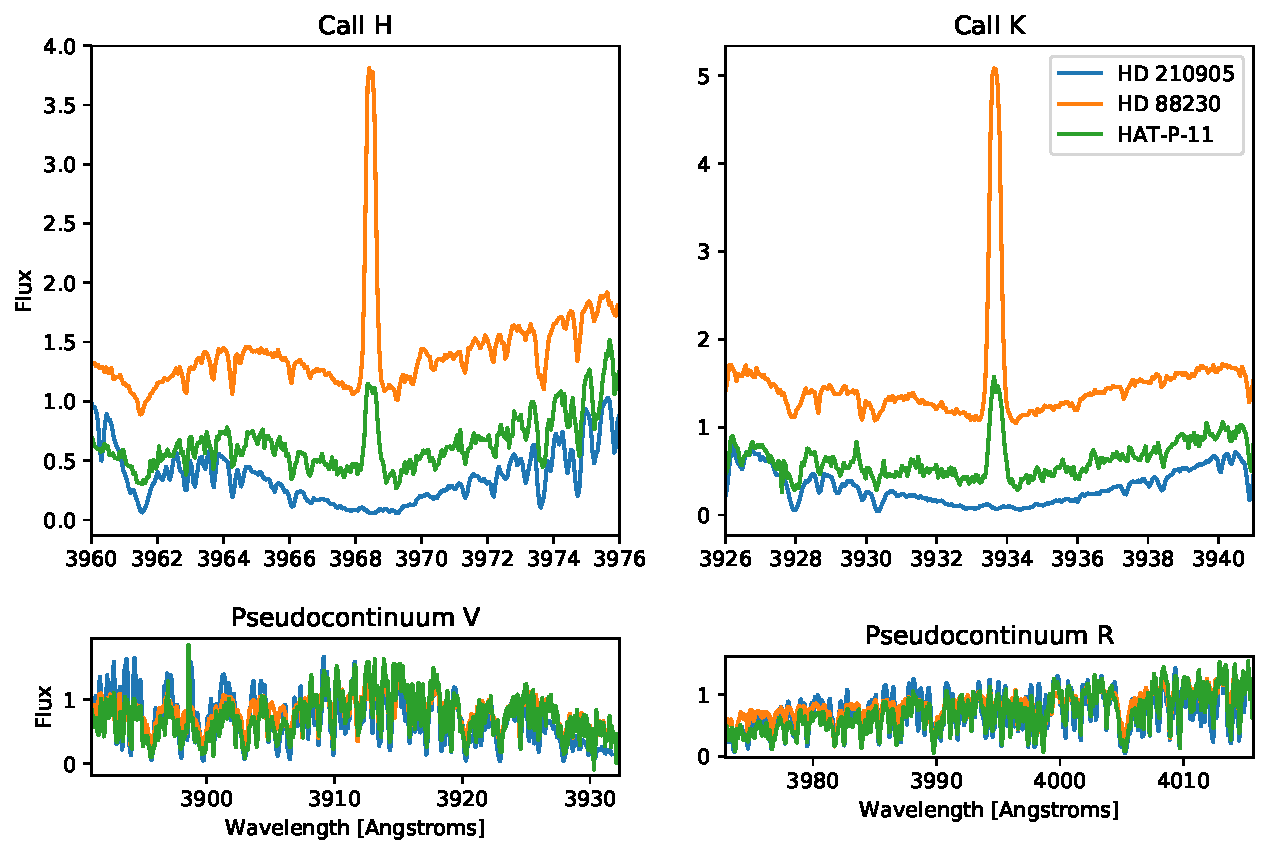
\includegraphics[scale=0.7]{sindex/example_spectra.pdf}
\caption{Spectra of two CaII H \& K calibration targets on the high and low activity ends, and HAT-P-11 in the middle.}
\label{fig:examplespectra}
\end{figure}

To calibrate the ARCES spectra, we follow the calibration procedure developed in \citet{Isaacson2010} for HIRES. We collect 51 spectra of 30 stars in the \citet{Duncan1991} MWO sample with the ARC 3.5 m Telescope at APO and the ARCES spectrograph, including 22 K stars, 7 G stars and one M star -- see Figure~\ref{fig:examplespectra} for example spectra. 

We measure the $S$-index for these stars by taking the sum of the flux in the cores of the $H$ and $K$ features at 3968.47 \AA\ and 3933.66 \AA, weighted with a triangular weighting function with FWHM=$1.09$\AA. We normalize the weighted emission by the flux in pseudocontinuum regions $R$ and $V$, which are 20 \AA-wide bands centered on 3900 and 4000 \AA, respectively. Then $S$ on the MWO-calibrated scale is 
\begin{eqnarray}
S_{APO} &=& \frac{a~H + b~K}{c~R + d~V} \\
S_{MWO} &=& C_1 S_{APO} + C_2, \label{eqn:s_ind}
\end{eqnarray}
where $a,~b,~c,~d, ~C_1$ and $C_2$ are parameters that can be tuned to make ARCES $S$-indices match the scale of $S_{MWO}$ \citep{Duncan1991}. Following the example of \citet{Isaacson2010}, we chose values of $a,b,c,d$ so that $S$ has roughly equal flux contributions from the $H$ and $K$ emission lines, and roughly equal flux from the $R$ and $V$ psuedocontinuum regions in the APO spectra. Thus we set $a = c = 1$, and we choose $b=2$ and $d=1$, so that $H \sim b~K$ and $K \sim d~V$. 

Since $S$ varies over time for each star in the sample, the linear correlation between the $S_{APO}$ and $S_{MWO}$ will have some intrinsic spread. To incorporate this into our model, we adopt the $\left< S \right>$ and the standard deviation of $S$ from \citet{Duncan1991} as the measurement and uncertainty of the MWO values. We solve for the constants $C_1$ and $C_2$ and their uncertainties with Markov Chain Monte Carlo (MCMC) \citep{Goodman2010, Foreman-Mackey2013}; the results are shown in Figure~\ref{fig:calib}. We find $C_1 = 21.26_{-0.83}^{+0.99}$ and $C_2 = 0.009_{-0.009}^{+0.011}$. The $S$-indices for each target are enumerated in Table~\ref{tab:cals}. The software tools used to calculate calibrated $S$-indices with spectra from ARCES are publicly available \footnote{\url{https://doi.org/10.5281/zenodo.886629}}.

\begin{figure}
\begin{center}
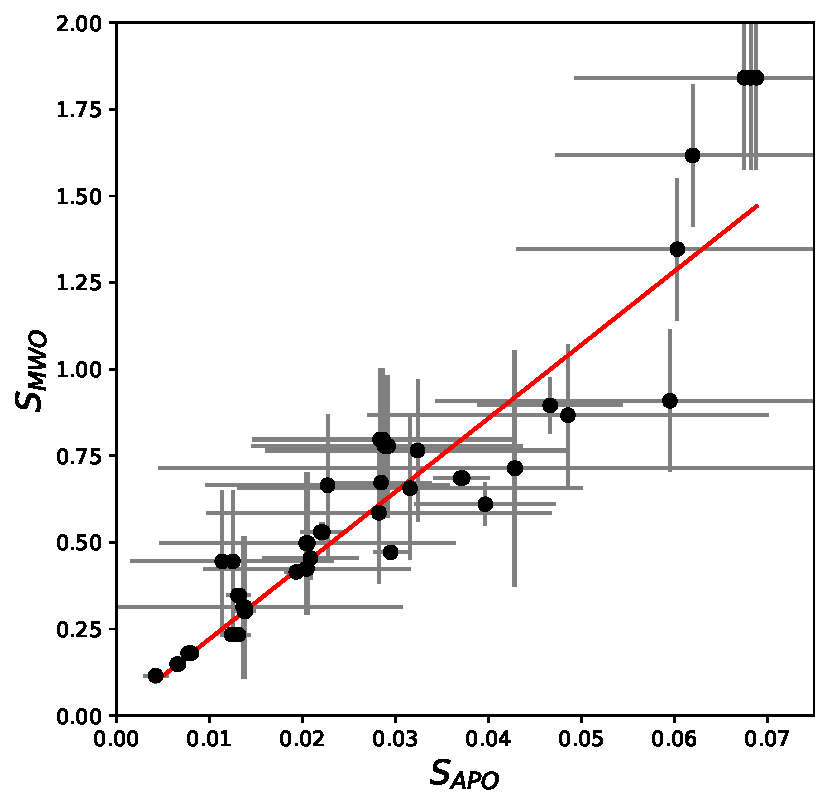
\includegraphics[scale=0.8]{sindex/s-index_calibration.pdf}
\caption{We calibrate the $S$-index measured with the APO echelle spectra against previous measurements from Mount Wilson Observatory (MWO) \citep{Duncan1991}. The large uncertainties in the MWO measurements are a result of the intrinsic activity variation of each star, and the uncertainties of the APO observations correspond to the measurement uncertainties.}
\end{center}
\label{fig:calib}
\end{figure}

\subsection{The $S$-index of HAT-P-11} \label{sec:s_h11}

\begin{figure}
\centering
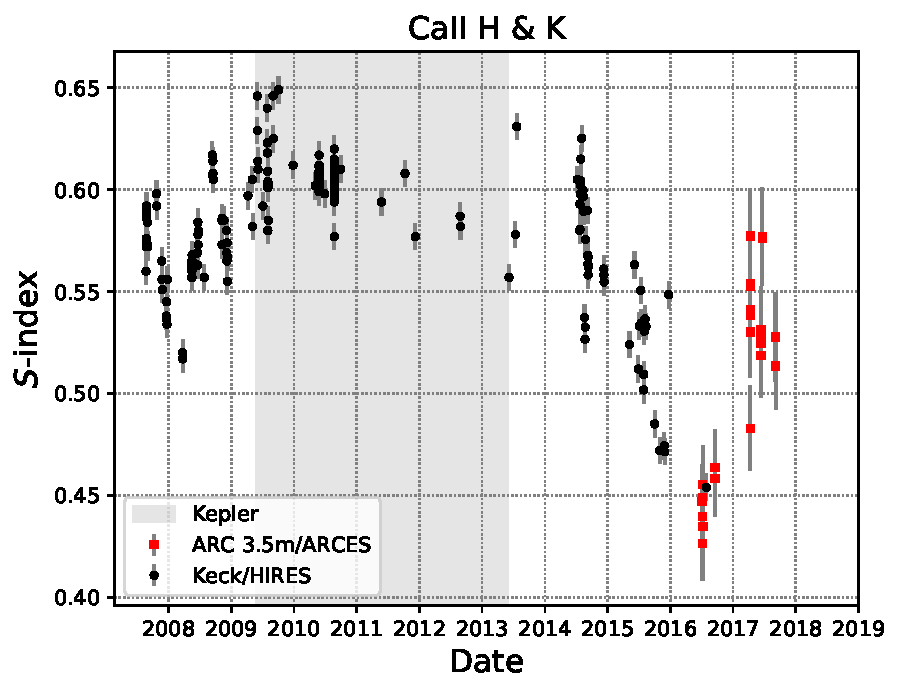
\includegraphics[scale=0.7]{sindex/s-index_hat11.pdf}
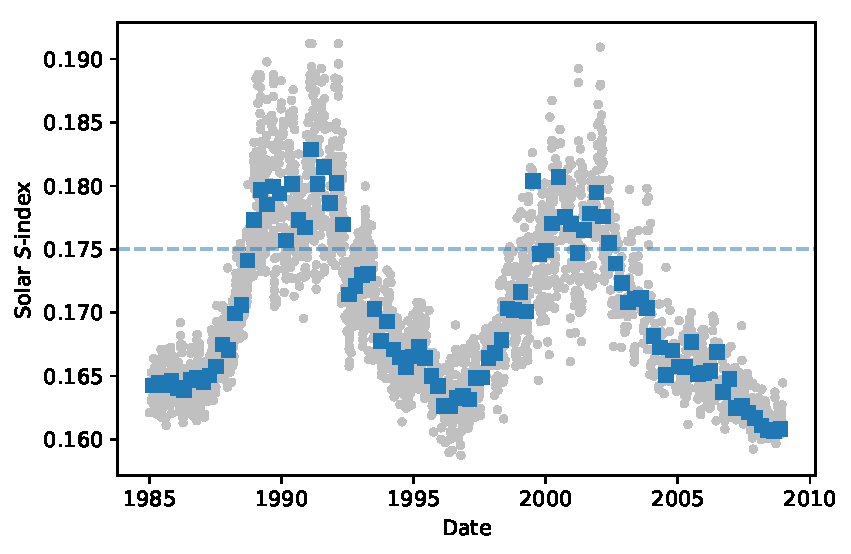
\includegraphics[scale=0.7]{sindex/solar_sind.pdf}
\caption{\textit{Upper:} $S$-index of HAT-P-11 over time with archival Keck/HIRES spectra and calibrated APO spectra from this work. We see evidence for an activity cycle with period $\sim$10 years or more. \textit{Lower:} the $S$-index of the Sun, from the National Solar Observatory (NSO) Integrated Sunlight Spectrometer (ISS) on the Synoptic Optical Long-term Investigations of the Sun (SOLIS) telescope. We convert the ISS CaII $K$ line fluxes to $S$-indices with Eqns.~5 and 12 of \citet{Egeland2017}. If we have observed nearly one complete activity cycle of HAT-P-11, it appears that HAT-P-11 spends a longer fraction of the cycle near activity maximum than the Sun does.}
\label{fig:activity_cycle}
\end{figure}

With the transformation computed in the previous section, we can compare the APO $S$-index measurements with those from the archival Keck/HIRES spectra. HAT-P-11 was the target of several Keck/HIRES programs since the planet's discovery, with the aims of measuring the Rossiter-McLaughlin effect and searching for a third body\footnote{We use archival spectra from program PIs: Bakos, D.~Bayliss, Beichman, Borucki, P.~Butler, D.~Fischer, Ford, Fortney, J.~Fuller, Gaidos, Hillenbrand, Howard, J~Johnson, Knutson, Mandushev, Marcy, Rogers, Sanchis-Ojeda, S.~Vogt}. We measure $S$-indices from these observations with the HIRES activity pipeline described in \citet{Isaacson2010}. A complete description of the HIRES pipeline developed for these measurements is beyond the scope of this paper; we refer the reader to \citet{Isaacson2010} for the full description. The result is an unevenly-sampled series of 239 $S$ measurements spanning 2007-2016, with typical $S/N \sim 20$. 

Figure~\ref{fig:activity_cycle} shows the $S$-index of HAT-P-11 between 2008-2017, including both the APO and Keck spectra. The APO $S$-indices are enumerated in Table~\ref{tab:sind}.The black circles are measurements from Keck/HIRES, and the red circles are measurements from APO. The chromospheric activity of HAT-P-11 appears to ramp up in the years preceding the \kepler\ mission, stabilize near a maximum throughout the \kepler\ years from 2009-2014, and then decline rapidly from 2014-2016 before rising at a similar rate through the present. 

Activity indices like $S$ vary on two timescales -- one driven by the rotation period of the star (29.2 d) as active regions rotate into and out of view, and the longer timescale throughout the activity cycle. It appears from this limited time series that HAT-P-11 may have entered activity maximum near the beginning of the \kepler\ observations. It is interesting to note that \citet{Morris2017} found that the starspots of HAT-P-11 are distributed in active latitudes centered on $\bar{\ell} = 16 \pm 1^\circ$, similar to the distribution of sunspots near solar activity maximum. The $S$-index appears to corroborate that if HAT-P-11's activity cycle is similar to the Sun's, it was at active maximum during the \kepler\ years.

Further spectroscopic monitoring will be required to determine the period of the activity cycle of HAT-P-11. During the summer of 2017, we measure $\left< S\right>_{2017} = 0.54 \pm 0.04$, still less than the earliest available measurements from the summer of 2007 $\left< S\right>_{2007} = 0.569 \pm 0.006$ -- it appears that one complete activity cycle has not yet elapsed. This gives a lower limit on the activity cycle period of $\sim 10$ years. The solar activity cycle is not perfectly periodic; the mean cycle duration and standard deviation are $10.9 \pm 1.2$ years \citep{Hathaway2002}. This lower limit on the activity cycle of HAT-P-11 observed thus far is longer than some solar activity cycles, but not longer than the mean. In principle one could attempt to measure the period of HAT-P-11's cycle by invoking empirical models of $S$ inspired by the solar activity cycle. However, as we will discuss below, HAT-P-11's $S$-index distribution with time departs from the typical $S$ distribution of the Sun -- HAT-P-11 spends more time near active maximum than minimum. Therefore we can only constrain a lower limit on the period with the observations thus far, and refrain from attempting to fit for the cycle period. 

The activity minimum of HAT-P-11 was short compared to its maximum. We note the marked difference between HAT-P-11 and the Sun in this respect in Figure~\ref{fig:activity_cycle}. Since we have not yet measured a full activity cycle of HAT-P-11 and the time sampling is very uneven, it is difficult to make concrete statements about the true duration of its maximum or minimum. One quantity that might be robust against these biases is the fraction of the activity cycle spent above or below the mean of $S_{min}$ and $S_{max}$, assuming the minimum and maximum observed $S$ are close to the true minimum and maximum of $S$ throughout the cycle. The Sun spends 25\% of the cycle above $0.5 (S_{min} + S_{max}) = 0.174$. The same quantity for HAT-P-11 is $0.5 (S_{min} + S_{max}) = 0.53$, and its $S$ was above that value from around or before 2008 until mid-2015, and stayed below that value until mid-2017. It appears that HAT-P-11 spent 63\% of its cycle above the mean of $S_{min}$ and $S_{max}$, assuming an $\sim 11$ year cycle. 

If HAT-P-11 has an $\sim 11$ year activity cycle, it falls in a sparse region of rotation period-cycle period parameter space. \citet{Bohm-Vitense2007} showed that stars typically fall into one of two categories: the young, active $A$-sequence, and old, inactive $I$-sequence (see \citealt{Bohm-Vitense2007} Fig.~1). $A$-sequence stars typically have ratios of cycle periods to rotation periods $P_{cyc}/P_{rot} \sim 360$, and $I$-sequence stars have $P_{cyc}/P_{rot} \sim 80$.  The Sun is a notable outlier residing in between the sequences with $P_{cyc}/P_{rot} \sim 160$. If HAT-P-11's activity cycle is roughly $\sim 11$ years, it is interesting to note that it has $P_{cyc}/P_{rot} \sim 139$, and it falls between the $A$ and $I$ sequences, like the Sun.

The APO spectra in Figure~\ref{fig:h} demonstrate that the activity has increased significantly in just the last two years. If we assume the cycle has a period of $\sim$11 years, we expect the next maximum to begin near 2019-2020. We predict that TESS photometry of HAT-P-11 will show spot occultations similar to those observed during the \kepler\ mission.

\begin{figure}
\begin{center}
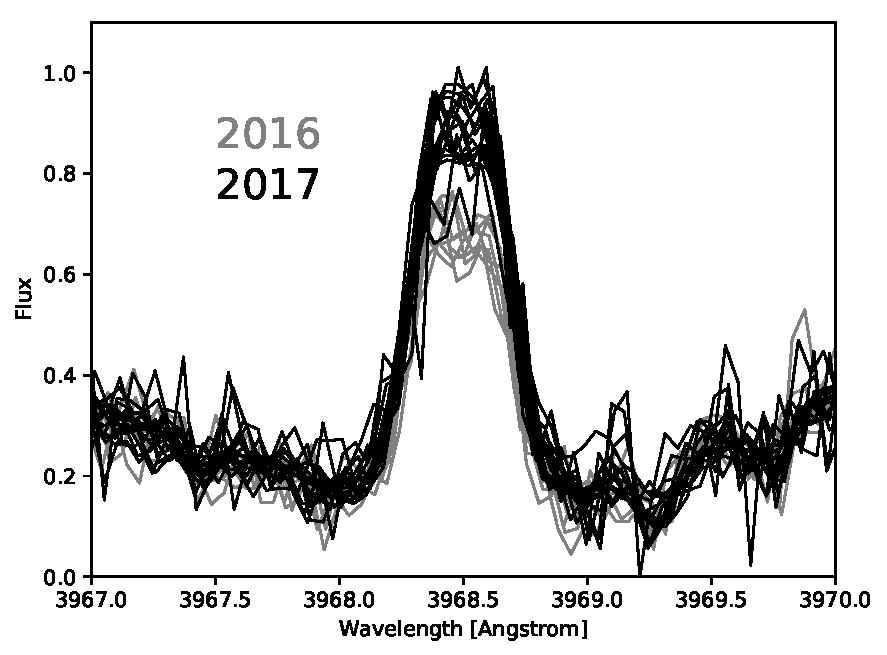
\includegraphics[scale=0.8]{sindex/close_up_h.pdf}
\end{center}
\caption{The CaII H feature of HAT-P-11 shows clear evolution towards more activity from 2016 to 2017 in the APO spectra. It appears that the activity may be approaching its maximal level as of mid-2017.}
\label{fig:h}
\end{figure}

\section{\kepler\ Full-frame image photometry} \label{sec:ffi}

\citet{Montet2017} searched for long term variability of \kepler\ targets in photometry from the full-frame images (FFIs). These were special exposures where the entire \kepler\ detector was read-out, whereas the short and long cadence photometry from \kepler\ was only telemetered for a small subset of the pixels. There were eight FFIs in 2009 during commissioning, and then approximately one per month for the remainder of the mission.

We use HAT-P-11 as a test-case for the reliability of long-term trends in FFI photometry, see Figure~\ref{fig:ffi}. The FFI photometry shows that the flux of HAT-P-11 varied by $\sim 2\%$ from 2009-2013 without a significant secular trend. The scatter in the FFI photometry is consistent with the scatter in the short-cadence SAP fluxes due to rotational variability of the star. Note that one should only compare the global scatter of the FFI and SAP fluxes to one another, and one should not expect the SAP light curve to perfectly intersect with the SAP measurements, since the SAP fluxes shown in Figure~\ref{fig:ffi} are normalized by the median flux of each quarter, and the FFI fluxes are normalized by the median flux over all FFIs. 

The $S$-index in Figure~\ref{fig:activity_cycle} indicates that HAT-P-11 had nearly uniform chromospheric emission throughout the years of the \kepler\ mission. Both the \kepler\ photometry and $S$-index are consistent with an active maximum period from 2009-2013.

The long term photometric variability of most Sun-like stars with rotation periods of 29 d is dominated by bright faculae \citep{Montet2017}. Future space-based photometry missions could therefore expect to measure a small dimming of the star during its short activity minimum.

\begin{figure}
\begin{center}
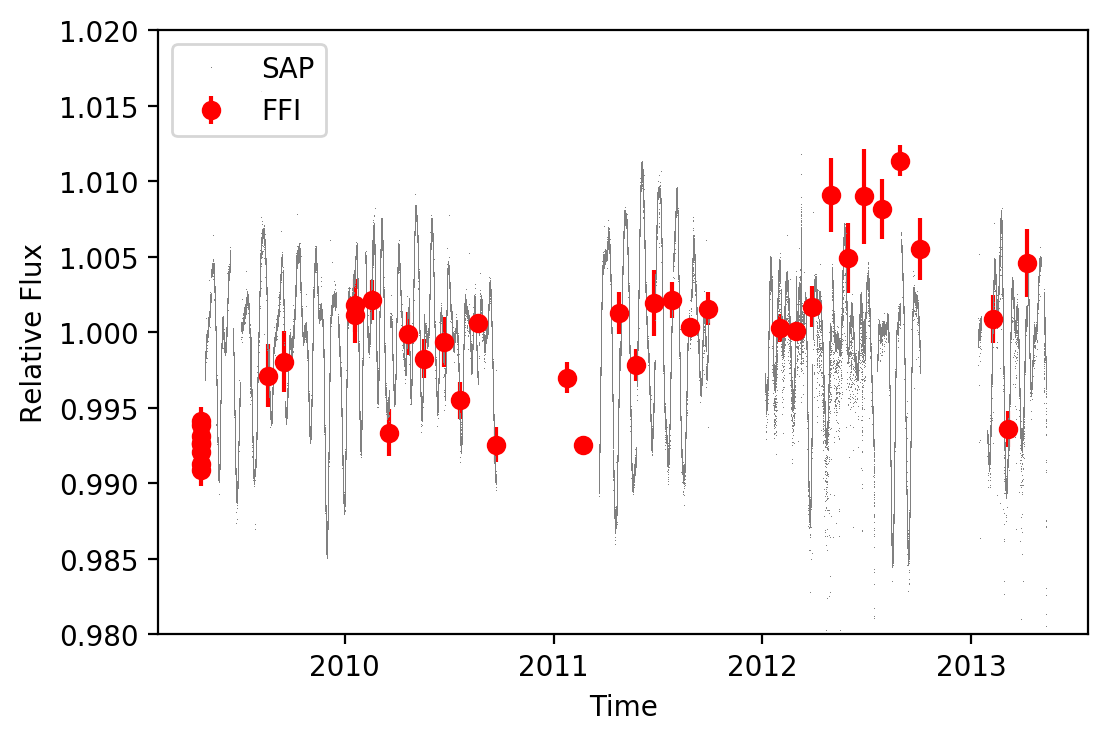
\includegraphics[scale=0.8]{sindex/ffi.png}
\end{center}
\caption{Full-frame image photometry of HAT-P-11 (red circles) and \kepler\ SAP one minute cadence fluxes (gray). \citet{Montet2017} searched for evidence of stellar activity cycles in the full-frame image (FFI) photometry. The $S$-index was near maximum throughout the \kepler\ mission, so we expect the FFI photometry to show scatter consistent with the 2\% rotational modulation in the \kepler\ short-cadence light curve. The FFI photometry indeed show scatter consistent with the rotational variability, without a significant secular trend.}
\label{fig:ffi}
\end{figure}

\section{HAT-P-11 in context} \label{sec:cks}

\subsection{Comparison to stars of similar color} \label{sec:mittag}

Is the chromospheric activity of HAT-P-11 typical for K4 dwarfs? The photometric analysis by \citet{Morris2017} can't be reproduced for many other \kepler\ stars. HAT-P-11 is exceptionally bright ($V=9.59$), and the highly inclined orbit of its planet reveals the latitude distribution of spots during transit events. Since very few similar targets are available for comparison in the \kepler\ sample, we seek to compare the spectrum of HAT-P-11 to spectra of other stars.

The $S$-index varies with stellar effective temperature, so the large $S$ of HAT-P-11 compared to the Sun does not imply that HAT-P-11 has more chromospheric activity than the Sun. The \rprime\ index is often used instead to compare activity levels across the main sequence, by normalizing the flux in the CaII H \& K emission features by the basal flux from the photosphere \citep{Noyes1984}. For stars of any effective temperature, \rprime\ increases with chromospheric activity.

We compute the \rprime\ index for a large sample of main sequence stars, following the procedure of \citet{Mittag2013}. We gathered published $S$-indices from \citet{Duncan1991}, \citet{Wright2004} and \citet{Isaacson2010}. As in \citet{Mittag2013}, we select only main sequence stars with color and absolute magnitude cuts using Hipparcos parallaxes \citep{Perryman1997}, yielding a sample of 4677 main sequence stars with measured $S$-indices. We then solve for \rprime\ for each star. We also compute \rprime\ for HAT-P-11 using its mean $\left < S \right> = 0.58 \pm 0.04$.

\begin{figure}
\begin{center}
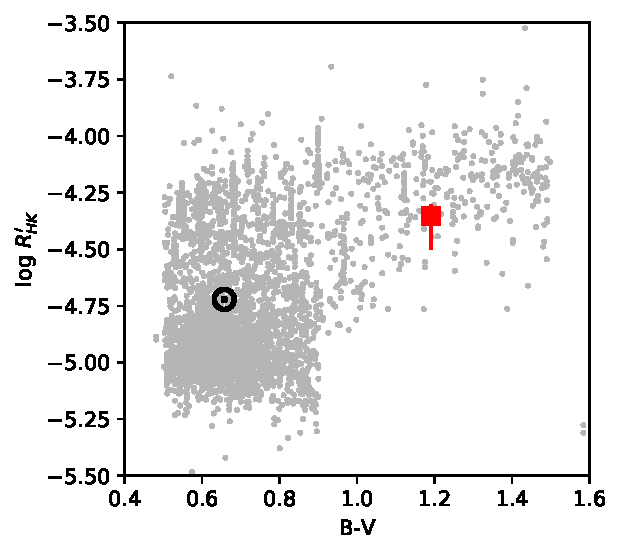
\includegraphics[scale=1]{sindex/rprime.pdf}
\end{center}
\caption{The \rprime\ index of HAT-P-11 (red square) among other main sequence stars (circles). The Sun is represented by the black ``$\odot$'' symbol, and resides on the the inactive branch of bluer stars. The distribution of \rprime\ at a given $B-V$ color is dominated by variation with age. Dwarfs with $B-V > 1$ typically have more active chromospheres than dwarfs with $B-V <1$. The errorbars on the square representing HAT-P-11 denote the minimum and maximum \rprime\ given the complete range of observed $S$ values throughout the activity cycle.}
\label{fig:rprime_ms}
\end{figure}

The \rprime\ index for each star in the literature is shown in Figure~\ref{fig:rprime_ms}. The characteristic rise in chromospheric activity for later type stars is visible in the right half of the figure. HAT-P-11 is the red square with $B-V = 1.19$ and $\log R^\prime_{HK} = -4.35$ (evaluated for $\left<S\right>$). The Sun is represented with the $\odot$ symbol and resides in the inactive sequence, blueward of HAT-P-11. 

HAT-P-11 has typical chromospheric activity among field stars of similar color. It lies near the lower envelope of \rprime\ at $B-V\sim1.2$, which one might expect given its rotation period $P_{rot} = 29.2$ d since \rprime\ declines with increasing age and rotation period \citep{Noyes1984}. HAT-P-11 also hosts a close-in planet which one might speculate could affect its activity, and in general we don't know the planet occurrence frequency in this sample of stars. As a result, it is perhaps more interesting to compare the chromospheric activity of HAT-P-11 to planet-hosting stars of similar color \textit{and} age.

\subsection{Comparison to planet hosts of similar color and age}

\begin{figure}
\begin{center}
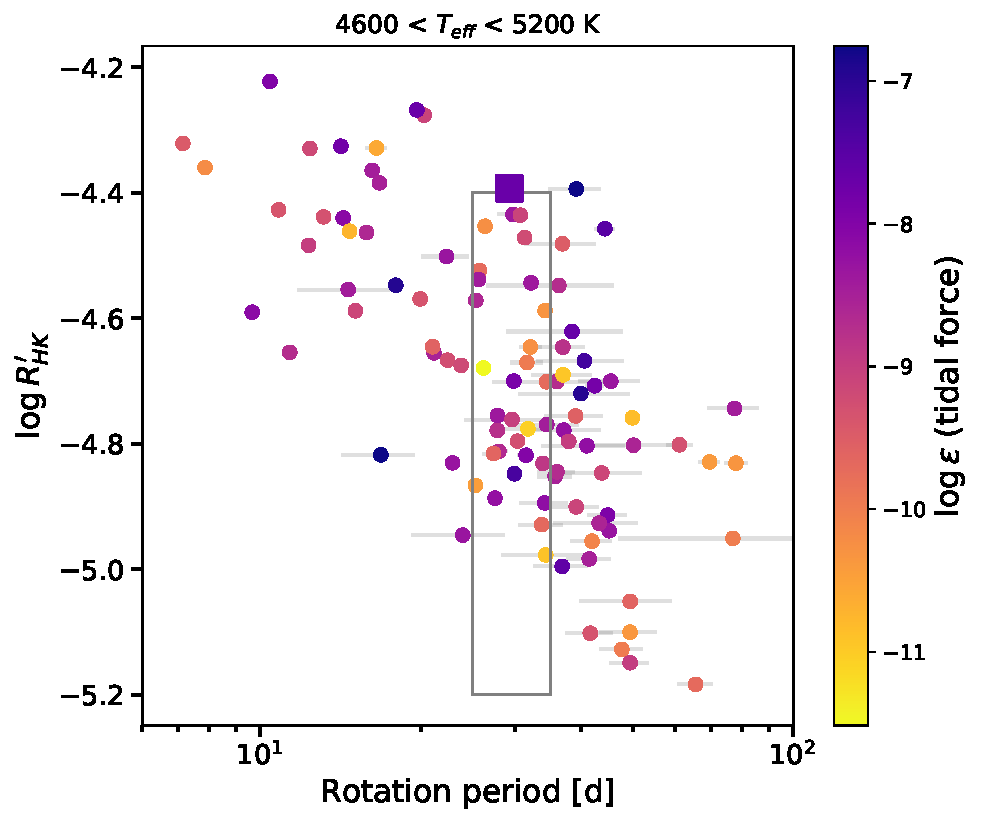
\includegraphics[scale=0.8]{sindex/cks_activity.pdf}
\end{center}
\caption{The \rprime\ index of HAT-P-11 (big square) among other main sequence planet-hosting stars (circles). HAT-P-11 is among the most active planet-hosting K stars with rotation periods near 30 d -- its \rprime\ is similar to the median \rprime\ for stars with rotation periods near $\sim 15$ days.}
\label{fig:cks_activity}
\end{figure}

Is the chromospheric activity of HAT-P-11 typical for planet-hosting K stars with long rotation periods? We build a sample of stars with similar effective temperatures to HAT-P-11 from the California-Kepler Survey (CKS), in which \citet{Petigura2017} published Keck/HIRES spectra and \citet{Johnson2017} published precise stellar parameters for 1305 planet-hosting \kepler\ stars.  We gather the CKS spectra of 107 planet-hosting stars which meet the following criteria: they have (1) effective temperatures in the range $4600 < T_{eff} < 5200$ K \citet{Petigura2017}, bracketing HAT-P-11 at $T_{eff} = 4780 \pm 50$ K \citep{Bakos2010}; (2) innermost planets with orbital periods $<20$ days; and (3) $S/N > 50$, where we approximate $S/N$ by dividing the median flux in the blue spectrum by the median uncertainty in the public CKS spectra.

We replicate the procedure in Section~\ref{sec:s_apo} to calculate $S$-indices for the CKS stars using the HIRES correction coefficients from \citet{Isaacson2010}, and use the relations of \citet{Mittag2013} to compute \rprime\ indices for each star as in Section~\ref{sec:mittag}. We also gather rotation periods for each star from \citet{Mazeh2015}, and we compute the Rossby number for each star with convective turnover times computed from the relations of \citet{Wright2011}.

We are particularly interested in whether or not HAT-P-11 experiences unusual planet-induced tides, which could provide a coupling between the planet's orbit and stellar activity. To quantify the relative tidal force on each star at the seat of stellar activity, the base of the convective zone, we use the simple dimensionless parameter $\epsilon$, 
\begin{equation}
\epsilon = \frac{M_p}{M_\star} \left( \frac{R_c}{a}\right)^3
\end{equation}
where $M_p$ and $M_\star$ are the masses of the planet and star, $R_c$ is the radius of the convective zone, and $a$ is planet's orbital semi-major axis \citep{Ogilvie2014}. The above equation is the ratio of the tidal force of the planet at the base of the convective zone $F_{tide} \propto M_p R_c / a^3$ to the local force of gravity within the star $F_g \propto M_\star / R_c^2$. This simple ratio does not take into account other likely important factors like the stellar obliquity. However, in the vast majority of cases the stellar obliquity is not known, so we continue to investigate tides with the imperfect index $\epsilon$, and discuss the implications of this caveat below.

We evaluate the tidal $\epsilon$ for the innermost planet in each system. We adopt the stellar radii and semi-major axes from the isochrone fits of \citet{Johnson2017}. We estimate the radius of the convective zone for each star by interpolating between the convective zone radii of model stars by \citet{vanSaders2012} of solar metallicity with $4600<T_{eff}<5200$ K. Finally, we adopt the mass measurement for HAT-P-11 b, $M_p=0.081 M_J$ from \citet{Bakos2010}, and estimate the most probable mass for all other planets using the \texttt{forecaster} tool by \citet{Chen2017}, given the measured planetary radii from \citet{Johnson2017}.

We recover the canonical result that \rprime\ generally decreases with rotation rate (or age) in Figure~\ref{fig:cks_activity}. It appears that HAT-P-11 (large square) has more chromospheric activity than other planet-hosting stars of similar rotation periods and effective temperatures. The gray box in Figure~\ref{fig:cks_activity} circumscribes 31 stars with rotation periods $25 < P_{rot} < 35$ d. The median activity level within the box is only 40\% of HAT-P-11's, $\log R^\prime_{HK} = -4.75$.

\subsection{The possible role of tides}

\begin{figure}
\begin{center}
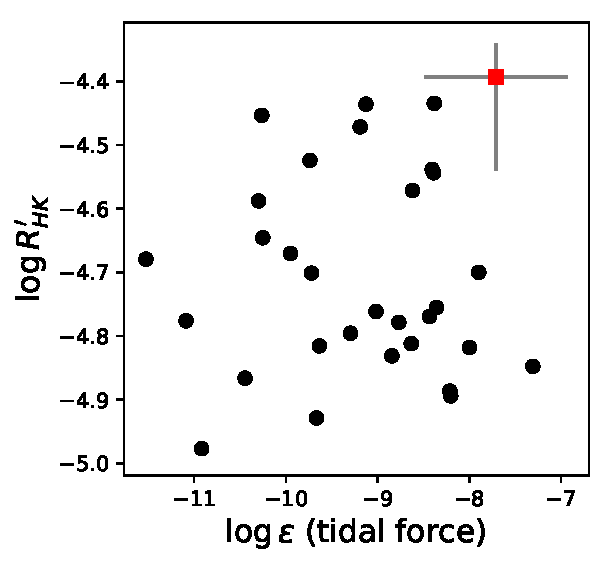
\includegraphics[scale=1]{sindex/tides_rhk.pdf}
\caption{The \rprime\ index for stars within the gray box in Figure~\ref{fig:cks_activity}, with rotation periods $25 < P_{rot} < 35$ d and effective temperatures $4600 < T_{eff} < 5200$ K. HAT-P-11 (red square) has the most activity in this bin, and the second-greatest tidal force on the base of its convective zone. The uncertainty in \rprime\ on HAT-P-11 represent its variation throughout its activity cycle. The uncertainty in $\epsilon$ on HAT-P-11 represents the characteristic uncertainty for all systems, which is dominated by uncertainty in the planet mass-radius relation of \citet{Chen2017}.}
\label{fig:rhk_eps}
\end{center}
\end{figure}

Could the relatively high level of chromospheric activity on HAT-P-11 (for stars with its age and color) be related to the tides raised by the close-in planet? We show the $\epsilon$-\rprime\ distribution of stars with $25 < P_{rot} < 35$ d in Figure~\ref{fig:rhk_eps}. We note that in this range of rotation periods, HAT-P-11 (red square) has the most chromospheric activity and the second-greatest $\epsilon$. However, the lack of  correlation between \rprime\ and $\epsilon$ suggests: (1) the tidal force isn't the only important factor in setting the level of chromospheric activity; and (2) the simple parameterization of $\epsilon$ does not capture all of the relevant physics. 

Significant tides are raised by HAT-P-11 b, even when compared to solar system objects. We can compare it's $\log_{10}\epsilon = -7.7$ with more familiar systems. $\epsilon$ at the base of the solar convective zone due to tides raised by Mercury gives $\log_{10}\epsilon = -13$, much less than any of the systems in Figure~\ref{fig:rhk_eps}. The Earth-Moon system experiences more similar tides with $\log_{10}\epsilon = -7.3$, and the dimensionless tidal force on HAT-P-11 is significantly less than the Jupiter-Io tides, $\log_{10}\epsilon = -6.6$. The tides raised by HAT-P-11 b are significant, and may have non-negligible effects on the interior dynamics of the star.

\subsection{The possible role of stellar obliquity}

Why is there no correlation between tidal force and chromospheric activity in this sample? We investigate the system with the greatest $\epsilon$ in more detail. That system is KOI-1050 with $\log_{10}\epsilon=-7.2$. Its star has mass $M_\star = 0.83 M_\odot$, effective temperature $T_{eff}= 5068$ K and rotation period $P_{rot} = 29.9$ d. It is orbited by planet with radius $R_p = 1.85 R_\oplus$, orbital period $1.27$ d and forecasted mass $M_p = 4.4 M_\oplus$. \rprime\ of KOI-1050 is less than half of HAT-P-11's despite its larger $\epsilon$. 

The dimensionless tidal force $\epsilon$ does not account for the transfer of energy due to obliquity tides -- the result of additional torques in star-planet systems with planetary orbits that are highly misaligned with respect to the stellar spin. The amplitude of energy transfer due to obliquity tides is proportional to $\sin^2 \psi$, where $\psi$ is the angle between the orbital angular moment vector and the stellar spin axis \citep{Wisdom2004}. The high obliquity of HAT-P-11 $\psi = 106^\circ {}^{+15}_{-11}$ suggests that obliquity tides on HAT-P-11 will contribute additional dissipation of orbital energy, which is not reflected by $\epsilon$. Lacking measurements of the obliquity of the other systems in Figure~\ref{fig:rhk_eps} such as KOI-1050, the observations presented here are insufficient to comment on whether or not the high obliquity of HAT-P-11 is responsible for its greater \rprime\ activity index compared to KOI-1050, for example. Future measurements of spin-orbit misalignment of close-in planets with active host stars may allow us to link stellar activity to the tides raised by planets.

It is also possible that a weak correlation between $\epsilon$ and \rprime\ is obscured by the large uncertainties in the forecasted planet masses. The parameter with the largest uncertainty in the calculation for $\epsilon$ is the planet mass. The forecasted mass estimates from \citet{Chen2017} have large uncertainties which reflect both measurement uncertainty and intrinsic spread in the observed planetary mass-radius relation. For the planets in the sample considered here, the median uncertainty in the forecasted planet mass is 78\%, which contributes to uncertainty on the order of 1 dex in epsilon. Thus the typical uncertainty in our estimates of $\epsilon$ is significant compared to the range observed. Follow-up radial velocity or transit timing variation measurements are needed to better constrain planet masses, and thus their tidal influence on their host stars.

Alternative activity indicators have been used to search for evidence that tidal interactions stoke stellar activity \citep[see reviews by][]{wright2015, poppenhaeger2017}. For example, \citet{Poppenhaeger2014} and \citet{miller2015} found enhanced stellar coronal X-ray emission from host stars that are expected to have strong tidal interactions with their hot Jupiters. \citet{saar2001} measured the chromospheric emission in the CaII infrared-triplet over time for stars with hot Jupiters, and found that the emission did not fluctuate on the orbital period of the planet.

In addition to tidal interactions, close-in planets can also interact magnetically with their host stars. \citet{Cohen2010, Lanza2010} showed that star-planet magnetic interactions can affect the angular momentum evolution of host stars. These studies examined planets with orbit normals that were aligned or anti-aligned with the stellar spin. The magnetic interactions between the star and planet in the HAT-P-11 system -- with its planet in a polar orbit -- are worthy of further study, and beyond the scope of this paper.

\section{Conclusion}

We present $S$-indices for HAT-P-11 from 2008-2017, which show evidence of an activity cycle of duration $\gtrsim 10$ years. We detail the calibration procedure for measuring $S$-indices with the echelle spectrograph on the ARC 3.5 m Telescope at APO. If the activity cycle is $\sim 11$ years, we expect the star to remain highly active from the present until $\sim 2023$, thus TESS will be able to observe spot occultations throughout the active maximum.

If we interpret the local minimum in $S$ near mid-2016 to be the true activity minimum, it seems that HAT-P-11 spends a greater fraction of time at maximum ($\sim 63\%$)  than the Sun does ($\sim 25\%$). The brightness of HAT-P-11 throughout the maximum lasting from 2009-2014 is consistent with under-sampled rotational variability, and does not show a significant secular trend. 

Among all K dwarfs, the strength of HAT-P-11's chromospheric activity measured by \rprime\ is unremarkable. However, among planet-hosting dwarfs with similar rotation periods and effective temperatures, the chromosphere of HAT-P-11 is exceptionally active. We speculate that tides raised by the planet on the star may play a role in the atypical activity.


% \acknowledgments

% We gratefully acknowledge support from NSF grant AST-1312453. We thank Lauren Weiss, John Lurie, and Daniel Foreman-Mackey for helpful discussions. 

% JRAD is supported by an NSF Astronomy and Astrophysics Postdoctoral Fellowship under award AST-1501418. 

% Work by B.T.M. was performed under contract with the California Institute of Technology (Caltech)/Jet Propulsion Laboratory (JPL) funded by NASA through the Sagan Fellowship Program executed by the NASA Exoplanet Science Institute. C.M.S. acknowledges funding from the Kenilworth Fund of the New York Community Trust.

% Based on observations obtained with the Apache Point Observatory 3.5-meter telescope, which is owned and operated by the Astrophysical Research Consortium. IRAF is distributed by the National Optical Astronomy Observatory, which is operated by the Association of Universities for Research in Astronomy, Inc., under cooperative agreement with the National Science Foundation

% Some of the data presented herein were obtained at the W. M. Keck Observatory, which is operated as a scientific partnership among the California Institute of Technology, the University of California and the National Aeronautics and Space Administration. The Observatory was made possible by the generous financial support of the W. M. Keck Foundation. The authors wish to recognize and acknowledge the very significant cultural role and reverence that the summit of Maunakea has always had within the indigenous Hawaiian community.  We are most fortunate to have the opportunity to conduct observations from this mountain.

%\facility{KeckI:HIRES, APO/ARC, Kepler}

%\software{\texttt{ipython} \citep{ipython}, \texttt{numpy} \citep{VanDerWalt2011}, \texttt{scipy} \citep{scipy},  \texttt{matplotlib} \citep{matplotlib}, \texttt{astropy} \citep{Astropy2013}, \texttt{forecaster} \citep{Chen2017}}

% \appendix

\begin{subappendices}
\section*{Appendix}

\begin{longtable}{l l c c c} %[H]
%\begin{center}
\caption{Stars observed to calibrate the $S$-index. \label{tab:cals}}
%\begin{tabular}{l l c c c}
Star & Sp.~Type & $S_{MWO}$ & $S_{APO}$ & $N$ \\
\hline
HD 210905 & K0III & $0.092 \pm 0.013$ & $0.004 \pm 0.000027$ & 1 \\
HD34411 & G1V & $0.145 \pm 0.022$ & $0.007 \pm 0.000069$ & 2 \\
HD68017 & G3V & $0.174 \pm 0.024$ & $0.008 \pm 0.00011$ & 2 \\
HD98230 & G2V & $0.266 \pm 0.031$ & $0.012 \pm 0.000052$ & 2 \\
HD 217906 & M2.5II-IIIe & $0.284 \pm 0.033$ & $0.013 \pm 0.00017$ & 2 \\
HD 201251 & K4Ib-IIa & $0.292 \pm 0.034$ & $0.013 \pm 0.000085$ & 2 \\
HD110833 & K3V & $0.306 \pm 0.035$ & $0.014 \pm 0.0001$ & 2 \\
HD39587 & G0VCH+M & $0.308 \pm 0.035$ & $0.014 \pm 0.000091$ & 2 \\
HD134319 & G5V: & $0.432 \pm 0.033$ & $0.019 \pm 0.000069$ & 1 \\
HD41593 & K0V & $0.457 \pm 0.049$ & $0.020 \pm 0.00012$ & 2 \\
HD87884 & K0Ve & $0.458 \pm 0.06$ & $0.020 \pm 0.00018$ & 3 \\
HD 220182 & G9V & $0.467 \pm 0.035$ & $0.021 \pm 0.000051$ & 1 \\
HD47752 & K3.5V & $0.495 \pm 0.074$ & $0.022 \pm 0.00022$ & 4 \\
HD127506 & K3.5V & $0.508 \pm 0.038$ & $0.023 \pm 0.00014$ & 1 \\
HD 122120 & K5V & $0.633 \pm 0.046$ & $0.028 \pm 0.00014$ & 1 \\
HD200560 & K2.5V & $0.638 \pm 0.049$ & $0.028 \pm 0.00045$ & 1 \\
HD  82106 & K3V & $0.638 \pm 0.08$ & $0.028 \pm 0.00017$ & 3 \\
HD 79555 & K4V & $0.651 \pm 0.082$ & $0.029 \pm 0.00024$ & 3 \\
HD 129333 & G1.5V & $0.661 \pm 0.048$ & $0.029 \pm 0.000066$ & 1 \\
HD149957 & K5V & $0.708 \pm 0.057$ & $0.032 \pm 0.0007$ & 1 \\
HD148467 & K6V & $0.727 \pm 0.057$ & $0.032 \pm 0.00062$ & 1 \\
HD 218356 & K1IV(e)+DA1 & $0.834 \pm 0.085$ & $0.037 \pm 0.00022$ & 2 \\
GJ702B & K4V & $0.891 \pm 0.065$ & $0.040 \pm 0.00042$ & 1 \\
HD45088 & K3Vk & $0.963 \pm 0.097$ & $0.043 \pm 0.00028$ & 2 \\
GJ 9781A & K7 & $1.048 \pm 0.075$ & $0.047 \pm 0.00016$ & 1 \\
HD 113827 & K4V & $1.091 \pm 0.078$ & $0.049 \pm 0.00019$ & 1 \\
HD175742 & K0V & $1.339 \pm 0.095$ & $0.060 \pm 0.00034$ & 1 \\
HD151288 & K7V & $1.357 \pm 0.098$ & $0.060 \pm 0.00057$ & 1 \\
HD 88230 & K8V & $1.394 \pm 0.099$ & $0.062 \pm 0.00021$ & 1 \\
HD 266611 & K5V & $1.534 \pm 0.19$ & $0.068 \pm 0.00085$ & 3 \\
%\end{tabular}
%\end{center}
\end{longtable}

\begin{table}[H]
\begin{center}
\caption{$S$-index measurements of HAT-P-11 from the ARC 3.5 m Telescope Echelle Spectrograph (ARCES) at the Apache Point Observatory (APO), calibrated against the Mount Wilson Observatory $S$-index. \label{tab:sind}}
\begin{tabular}{ccc}
JD & $S$ & Uncertainty \\ \hline
2457572.9442 & 0.45 & 0.04 \\
2457575.9589 & 0.43 & 0.04 \\
2457576.8890 & 0.44 & 0.04 \\
2457576.8978 & 0.45 & 0.04 \\
2457576.9065 & 0.45 & 0.04 \\
2457578.9182 & 0.43 & 0.04 \\
2457649.6839 & 0.46 & 0.04 \\
2457649.6964 & 0.46 & 0.04 \\
2457854.8691 & 0.48 & 0.04 \\
2457854.8899 & 0.53 & 0.04 \\
2457854.9056 & 0.55 & 0.05 \\
2457854.9212 & 0.53 & 0.04 \\
2457854.9369 & 0.54 & 0.04 \\
2457854.9527 & 0.54 & 0.04 \\
2457854.9684 & 0.55 & 0.04 \\
2457854.9840 & 0.58 & 0.05 \\
2457916.8112 & 0.53 & 0.04 \\
2457916.8338 & 0.53 & 0.04 \\
2457916.8937 & 0.52 & 0.04 \\
2457916.9163 & 0.53 & 0.04 \\
2457916.9372 & 0.52 & 0.04 \\
2457924.8090 & 0.58 & 0.05 \\
2457924.8260 & 0.58 & 0.05 \\
2458001.6552 & 0.53 & 0.04 \\
2458001.6778 & 0.51 & 0.04 \\
\end{tabular}
\end{center}
\end{table}

\end{subappendices}


%\bibliographystyle{apj}
%\bibliography{./sindex/sindex_bibliography}



% \end{document}


\chapter{The Active Latitudes of HAT-P-11: Evidence for a Solar-like Dynamo}

% \documentclass[iop]{emulateapj}
% \documentclass[manuscript]{aastex61}
% \documentclass[preprint2]{aastex61}

% \submitjournal{Astrophysical Journal}
% \accepted{August 7, 2017}

% \usepackage{natbib}
% \bibliographystyle{humannat}

\newcommand{\stsp}{\texttt{STSP}\xspace}
\newcommand{\kepler}{\textit{Kepler}\xspace}
% \usepackage{amsmath}
% \usepackage{color}

% \shorttitle{HAT-P-11: Evidence for a Solar-like Dynamo}
% \shortauthors{Morris et al.}
% \submitjournal{ApJ}

% \begin{document}

% \title{The Starspots of HAT-P-11: Evidence for a solar-like dynamo}

% \author{Brett M. Morris}
% \affiliation{Astronomy Department, University of Washington, Seattle, WA 98119, USA}

% \author{Leslie Hebb}
% \affiliation{Physics Department, Hobart and William Smith Colleges, Geneva, NY 14456, USA}

% \author{James R. A. Davenport}
% \affiliation{Department of Physics \& Astronomy, Western Washington University, Bellingham, WA 98225, USA}
% \affiliation{NSF Astronomy and Astrophysics Postdoctoral Fellow}

% \author{Graeme Rohn}
% \affiliation{Physics Department, State University of New York at Cortland, Cortland, New York 13045-0900, USA }

% \author{Suzanne L. Hawley}
% \affiliation{Astronomy Department, University of Washington, Seattle, WA 98119, USA}

% \email{bmmorris@uw.edu}

% \begin{abstract}
% We measure the starspot radii and latitude distribution on the K4 dwarf HAT-P-11 from \kepler\ short-cadence photometry. We take advantage of starspot occultations by its highly-misaligned planet to compare the spot size and latitude distributions to those of sunspots. We find that the spots of HAT-P-11 are distributed in latitude much like sunspots near solar activity maximum, with mean spot latitude of $\approx 16 \pm 1^\circ$. The majority of starspots of HAT-P-11 have physical sizes that closely resemble the sizes of sunspots at solar maximum. We estimate the mean spotted area coverage on HAT-P-11 is $3^{+6}_{-1}\%$, roughly two orders of magnitude greater than the typical solar spotted area.
% \end{abstract}

% %\object{HAT-P-11}

% \keywords{starspots, sunspots, stellar activity, stellar activity cycles, Kepler photometry, stellar dynamo}

\section{Introduction}

The Sun is our local laboratory for understanding stellar magnetic activity. Centuries of sunspot observations and recent helioseismology results point towards the $\alpha\Omega$ dynamo mechanism as the source of solar magnetic activity. Solar magnetic fields are stored and amplified in poloidal and toroidal components, in the tachocline beneath the convective zone, until magnetic buoyancy causes them to rise. The buoyant magnetic flux tubes become visible as sunspots where they intersect with the photosphere \citetext{\citealp{Parker1955a, Parker1955b, Babcock1961}; \citealp[see reviews by][]{Charbonneau2010, Cheung2014, Hathaway2015}}. 

Magnetic activity on slowly rotating Sun-like stars is difficult to measure \citep{Saar1990} because the Sun has dark spots spanning only $\lesssim 0.5\%$ of its surface area at its most active, while spot areas of at least $\gtrsim 10\%$ are required to detect high S/N molecular absorption or Zeeman splitting. Polarization can characterize spots on resolved stars such as the Sun, but the opposite polarities in bipolar magnetic regions cancel one another in unresolved spot pairs, yielding little net polarization. As a result, most of our measurements of stellar activity come from stars much more active than the Sun \citep[see reviews by][]{Berdyugina2005, Reiners2012}.

Initial observations of a small sample of Sun-like stars show that the fraction of magnetic energy stored in the toroidal field decreases as rotation period increases \citep{Petit2008}. Spot temperatures and area covering fractions have been inferred from molecular absorption by TiO and OH in cool starspots of Sun-like stars \citep{Neff1995, oneal1996, ONeal2001, ONeal2004}.  The properties of sunspots that are most informative for constraining dynamo theory, such as the physical sizes and latitude distributions of spots, are typically highly degenerate with these observing techniques.

Transiting exoplanets enable measurements of spot sizes and positions on their host stars. During an exoplanet transit, the flux lost at any instant is proportional to the intensity of the occulted portion of the stellar surface. Occultations of starspots by exoplanets are observed as positive flux anomalies in transit light curves, which are resolved in time by \kepler\ short-cadence photometry. \cite{Hebb2017} develop a photometric model for spotted stars which computes the observed light curve for spots of a given size and position on the stellar surface. \stsp\ simulates times during transit -- when the planet may or may not be occulting a spot -- and during the rest of the planetary orbit when the stellar rotation drives photometric variability.

In this work, we will make a direct comparison between the Sun and an exoplanet host star using the occultation mapping method. We measure starspot positions and sizes using the photometric model \stsp\ developed in \citet{Hebb2017}. \stsp\ simulates photometric time series measurements for stars with spotted surfaces and transiting planets. If we know the stellar orientation relative to the planet's orbit, the timing and morphology of spot occultations can be transformed into precise positions of starspots with the forward-modeling approach of \stsp.

The active, transiting planet host star HAT-P-11 produces many spot occultations in its \kepler\ light curve -- see Figure~\ref{fig:transit_gallery} for examples. It is a K4 dwarf with a hot Neptune planet with orbital period $P = 4.88$ d, mass $M_p = 0.08 M_J$, and radius $R_p = 0.4 R_J$ \citep{Bakos2010}. Observations of the Rossiter-McLaughlin effect revealed that HAT-P-11 b likely orbits over the poles of its host star \citep{Winn2010, Hirano2011, Sanchis-Ojeda2011}. Therefore the transit chord of the planet sweeps a path across one stellar longitude over many latitudes. The stellar rotation period and the orbital period of the planet are nearly commensurate at 6:1, which causes transits to occur near the same six stellar longitudes \citep{Beky2014a}.

Spot crossings of HAT-P-11 in the \kepler\ observations can be used to search for active stellar latitudes. \citet{Sanchis-Ojeda2011} and \citet{Deming2011} noted that the first few quarters of \kepler\ observations show spot occultations predominantly at two orbital phases, which they attribute to starspots which are concentrated into two active latitudes. \cite{Beky2014b} constructed a spot occultation model which they applied to HAT-P-11, and they estimate spot contrasts and sizes.

We introduce the \stsp\ model and solve for the inputs it requires in Section~\ref{sec:inputs}, and measure spot positions and sizes in Section~\ref{sec:stsp}. We compare the spot sizes, active latitudes, and spotted area coverage of HAT-P-11 to the Sun in Section~\ref{sec:results}. Finally, we discuss the properties of HAT-P-11's activity in Section~\ref{sec:conclusion}. 

\section{Starspot Modeling: Inputs for \stsp} \label{sec:inputs}

\citet{Hebb2017} developed a flux model for spotted stars with transiting planets called \stsp, which leverages spot occultations during planetary transits to break the spot position degeneracies. They illustrated the mapping technique on the young solar-like star Kepler-17. The alignment of the stellar spin and planetary orbit in that system confine the spot occultation observations to one narrow band of stellar latitudes. This alignment allowed them to probe the time evolution of spots, since the same spot was occulted multiple times in consecutive transits. In the HAT-P-11 system, the near-perpendicular misalignment of the stellar spin and planetary orbit alternatively allows us to probe spot positions as a function of latitude.

We first need to determine several input parameters that will be fixed in the \stsp\ flux model, enabling us to solve for the spot properties. In Section~\ref{sec:transit}, we fit for the orbital properties of the planet from the transit light curves. We solve for the initial spot positions with a simplified spot model in Sections~\ref{sec:spotoccmodel}-\ref{sec:friedrich}, which enables us to measure the approximate stellar inclination in Section~\ref{sec:i_s}, re-evaluate the spin-orbit obliquity in Section~\ref{sec:obliquity}, and to test our assumptions about spot contrasts in Section~\ref{sec:contrast}. With the approximate starspot positions derived from the simplified model fits, we explore the spot latitude-longitude-radius parameter space with the full \stsp\ forward model in Section~\ref{sec:stsp}. 

\stsp\ is a pure \texttt{C} code for calculating the variations in flux of a star due to spots, both in- and out-of-transit  \citep{Hebb2017}. We use \stsp\ because its prescription for the shapes of spot occultations are more realistic than the simple model in Sections~\ref{sec:spotoccmodel}-\ref{sec:friedrich}, and the correlations between MCMC parameters allow us to properly explore the degeneracies between starspot positions and sizes. \stsp\ can also solve for the properties of spots driving out-of-transit flux modulations, however in this work we consider only the spots detected in-transit, since the spot occultations yield tighter constraints on the spot properties than the out-of-transit flux variations.

\subsection{Orbital Properties of HAT-P-11 \lowercase{b}} \label{sec:transit}

\begin{figure}
\centering
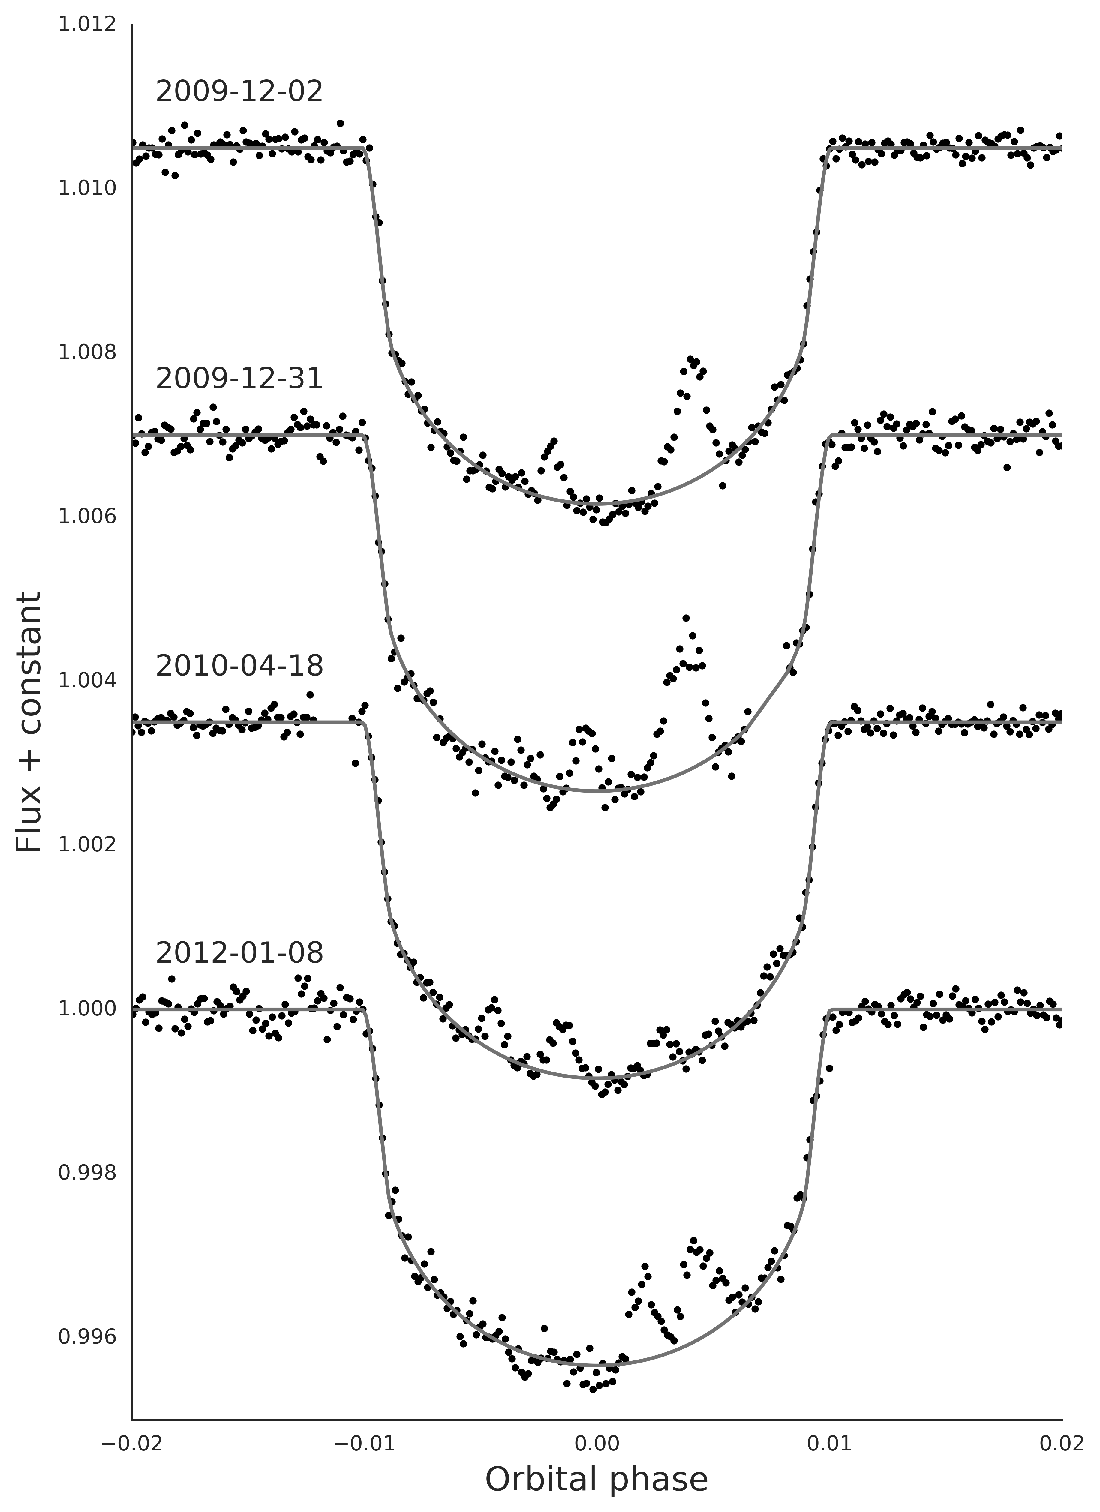
\includegraphics[scale=0.4]{stsp_hat_p_11/transit_gallery.pdf}
\caption{Typical transit light curves of HAT-P-11 b. The points are \kepler\ fluxes, the curves are the best-fit transit model \citep{Mandel2002}. The positive anomalies during transit are occultations of starspots by the planet.}
\label{fig:transit_gallery}
\end{figure}

To study the signal imparted by starspots on the transit light curve residuals, we must first remove the transit of HAT-P-11b from each light curve. It is non-trivial to derive the transit parameters for HAT-P-11 b since nearly all of the transits appear to be affected by starspots to some extent. We acknowledge that the most robust measurement of the transit properties would be obtained by fitting the light curve simultaneously for the transit and the occulted starspots, but the number of parameters in that fit is prohibitively large. Therefore, we opt to fit for the transit parameters on a subset of transits with minimal starspot anomalies, and to fix those transit parameters later when we fit for the starspot properties. In the next two sections, we outline the procedure for finding the orbital properties of HAT-P-11 b in spite of the abundant starspots.

\subsubsection{Light Curve Normalization} \label{sec:norm}

For the transit depths to be consistent in each transit light curve, an appropriate normalization for each transit must be chosen. Transit light curves are often normalized by the flux immediately before ingress and after egress. However, each transit light curve will have different relative depths if the total flux of the star is varying due to unocculted starspots \citep{Czesla2009, Carter2011, Csizmadia2013}. For example, if unocculted starspots dim the host star's flux by a factor $0 < \epsilon < 1$, the flux lost during transit $\Delta F$ is unaffected, but the total flux $\epsilon F$ is smaller, so the relative depth $\delta = \Delta F / (\epsilon F)$ is larger for the spotted star than for the unspotted star. The transits of HAT-P-11 likley have many occulted and unocculted starspots, and the transit depths would vary in time if simple out-of-transit flux normalization was used. In this section, we outline a normalization procedure that ideally yields transits of constant depth for stars with unocculted starspots, so that we can use a single depth parameter for all transits which corresponds to the square of the ratio of radii, $\delta \propto (R_p/R_s)^2$.

We assume that the peak flux of HAT-P-11 over a few stellar rotations is close to the unobscured brightness of the unspotted star\footnote{This assumption is revisited in the discussion in Section~\ref{sec:spotted_area}}. We then normalize all transit fluxes by: (1) fitting and subtracting a second-order polynomial to the out-of-transit Simple Aperture Photometry (SAP) fluxes near each transit; (2) adding the peak quarterly flux to each polynomial detrended transit; and (3) dividing each transit by the peak flux of each quarter. The subtraction by a second-order polynomial removes trends in flux due to stellar rotation, and the addition and division by the peak flux normalizes the out-of-transit fluxes to near-unity, while keeping the transit depths consistent between transits \citep{Hebb2017}. We must use the SAP flux because it is the unnormalized flux in units of electrons per second, rather than the PDCSAP flux which is already normalized.

\subsubsection{``Spotless'' Transits} \label{sec:spotless}

\begin{table}
\begin{center}
\begin{tabular}{lr}
Parameter & Measurement\\ \hline \hline
Orbital period [d] & $4.88780258 \pm 0.00000017$ \\
Mid-transit [JD] & $2454605.89146 \pm 0.000020$ \\
Depth $\approx \left(\frac{R_p}{R_*}\right)^2$ & $0.00340 \pm 0.00002$\\
Duration, $T_{14}$ [d] & $0.0980 \pm 0.0001$\\
$b$ & $0.141^{+0.052}_{-0.080}$ \\
$q_1 = (u_1 + u_2)^2$ & $0.48 \pm 0.01$ \\ 
$q_2 = \frac{u_1 }{2(u_1 + u_2)}$ & $0.46 \pm 0.01$ 
\end{tabular}
\end{center}
\caption{Transit light curve parameters for HAT-P-11 from the ten transits in Figure~\ref{fig:spotlesstransits}. $T_{14}$ is the duration between first and fourth contact; $q_1$ and $q_2$ are the limb-darkening parameters of \citet{Kipping2013}; $u_1$ and $u_2$ are the standard quadratic limb-darkening parameters. These parameters are fixed in the starspot fits.}
\label{tab:transitprops}
\end{table}

\begin{figure}
\centering
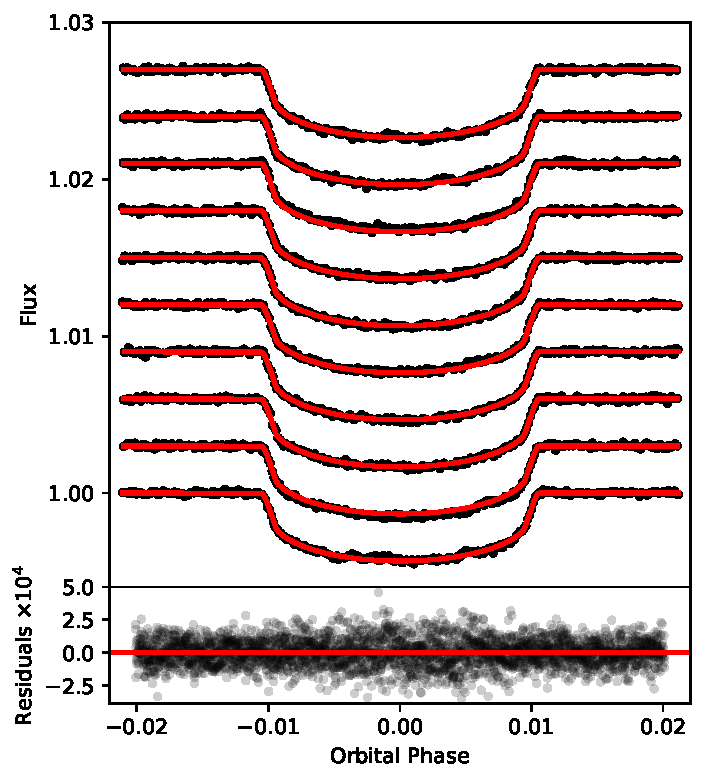
\includegraphics[scale=0.7]{stsp_hat_p_11/hat11_spotless_transits_compact.pdf}
\caption{The ten transits least affected by starspot crossings, which we fit for the planet orbital parameters listed in Table~\ref{tab:transitprops}.}
\label{fig:spotlesstransits}
\end{figure}

We select the ten transits with the fewest measurable starspot crossings to fit for the transit parameters. To identify the transits least perturbed by starspots, we fit a \citet{Mandel2002} transit light curve to each of the 205 normalized short-cadence transits in the full \kepler\ light curve. We hold the light curve parameters fixed, except for the depth which is allowed to vary, and optimize the light curve parameters using Levenburg-Marquardt least-squares minimization. We allow depth to vary because fits to transits with spot occultations (positive flux anomalies) will be biased towards smaller transit depths and higher $\chi^2$. We then select the ten transits with the smallest $\chi^2$. There are no significant starspot crossings visible by eye after this selection process, see Figure~\ref{fig:spotlesstransits}. 

We fit the ten transits for the orbital parameters and the stellar limb-darkening coefficients. We compute transit light curves with the \texttt{batman} package \citep{Kreidberg2015}, and sample the parameter posterior distributions with the affine-invariant Markov Chain Monte Carlo (MCMC) package \texttt{emcee} \citep{Foreman-Mackey2013}. The best-fit transit parameters are listed in Table~\ref{tab:transitprops}. 

The maximum likelihood planet-to-star radius ratio is $R_p/R_\star = 0.058 \pm 0.004$. This measurement is in agreement with \citet{Deming2011} ($0.0589 \pm 0.0002$), \citet{Southworth2011} ($0.058 \pm 0.001$), and \citet{Bakos2010} ($0.0576 \pm 0.0009$).

Measurements of the mean stellar density of HAT-P-11 via asteroseismology and transit light curves have been reported by \citet{Christensen-Dalsgaard2010} and \citet{Southworth2011}, respectively. Using our transit parameters for HAT-P-11 b, we constrain the mean stellar density $\rho_s = 1.81 \pm 0.04 \rho_\odot$, which is similar to the preliminary asteroseismic measurement of $\rho_s = 1.7846 \pm 0.0006 \rho_\odot$, and smaller than the previous photometric measurement, $2.415 \pm 0.097\rho_\odot$.

\subsection{Spot Position Initial Conditions} \label{sec:spotoccmodel}

\begin{figure}
\centering
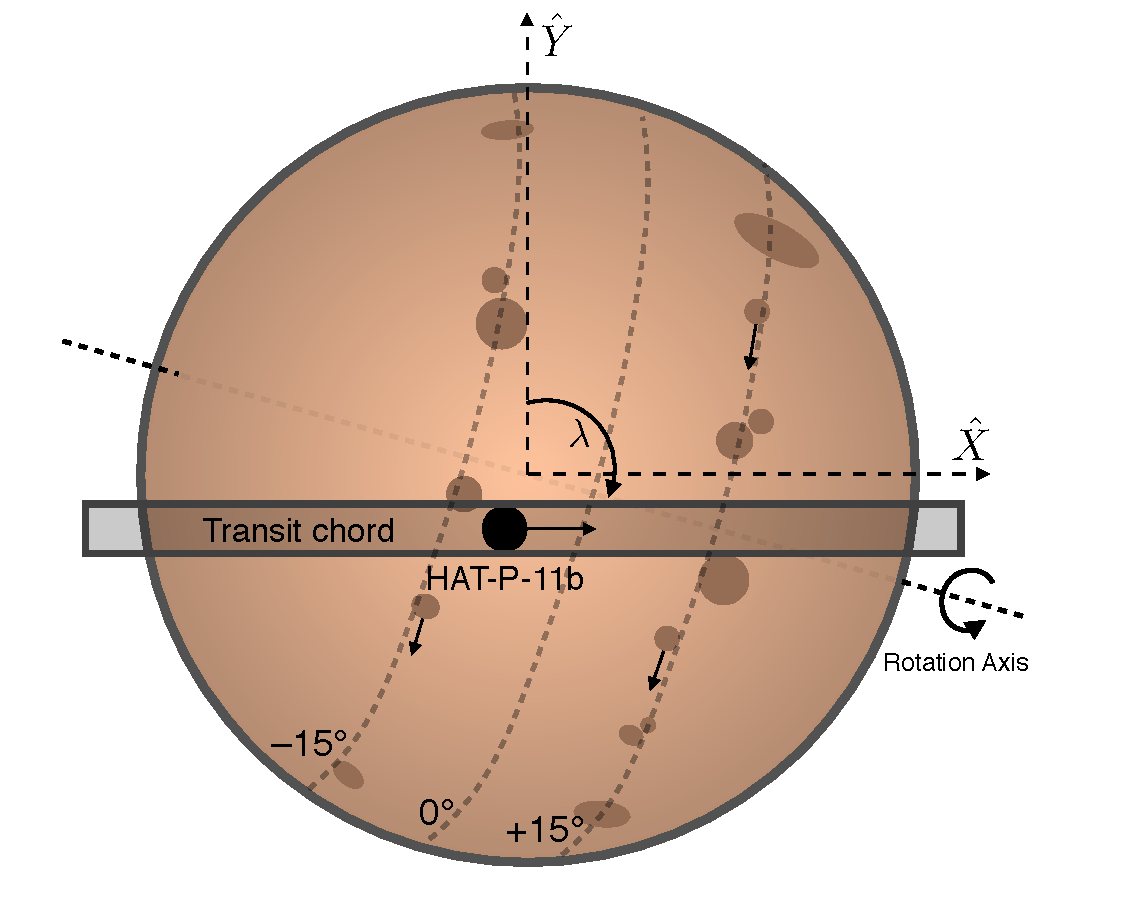
\includegraphics[scale=0.45]{stsp_hat_p_11/schematic.pdf}
\caption{The HAT-P-11 system in the observer-oriented coordinate system of \citet{Fabrycky2009}, roughly to scale. The planet's orbit is misaligned from the stellar rotation axis by the projected spin-orbit angle $\lambda = 106^\circ$ \citep{Sanchis-Ojeda2011}, and the north rotational pole of the star is inclined away from the observer by $i_s = 100^\circ$.}
\label{fig:schematic}
\end{figure}

We observe starspot occultations as positive flux anomalies during transit events. The amplitudes, durations and timing of the spot occultations constrain the spot locations and radii. If the starspot is a uniformly dark circular region on the star, and the planet passes over the edge of the spot in a grazing occultation, the resulting flux anomaly is an inverted ``v'' shape, analogous to the shape of an inverted eclipsing binary light curve. If the planet completely occults the spot or the spot completely circumscribes the planet, the resulting flux anomaly is an inverted ``u'' shape, like an inverted exoplanet transit event. There are many more grazing spot occultations (``v''-shaped, roughly approximated by Gaussians) than complete spot occultations. In most \kepler\ transits of HAT-P-11, there are between one and four spot occultations with amplitudes more than a few times the noise.

It is notoriously difficult to measure starspot positions robustly, because they are described by several degenerate quantities. For example, the occultation of a small, very dark spot is often degenerate with a larger spot of less extreme intensity contrast. These degeneracies can be broken for host stars of transiting exoplanets like HAT-P-11. The orientation of the planet's orbit is measured from the transit light curve, and the orbital phase of the planet at each time maps to a position on the projected stellar surface that is being occulted. We can measure the orientation of the star with two angles -- the spin-orbit angle which is measured via the Rossiter-McLaughlin effect, and the stellar inclination. We need to assume a stellar inclination, since the spectroscopic $v\,\sin{i}$ is consistent with zero \citep{Bakos2010} due to this star's long rotation period. \citet{Sanchis-Ojeda2011} found that active latitudes are evident in the spot positions recovered from the \kepler\ photometry, and they measure the stellar inclination by assuming that the active latitudes are symmetric with respect to the stellar equator. Using the same technique, we can then map the flux measured at a given time to the brightness of the stellar surface at a particular latitude and longitude. Then when the planet occults a dark starspot, the timing and shape of the positive flux anomaly in the transit light curve can be transformed into the position and radius of the starspot. 

Figure~\ref{fig:schematic} depicts the orientation of the system. HAT-P-11 b's orbit normal is nearly perpendicular to the host star's spin -- in other words, it nearly orbits over the host star's poles. Thus each transit cuts a chord across the stellar surface from pole to pole, across most latitudes and over a narrow range in longitude. The transit chords start near the southern rotational pole of the star in the eastern hemisphere, pass over the sub-observer meridian in the northern hemisphere, and end to the northwest of where the chord began. The most complete latitude coverage is from the equator to $\pm 50^\circ$, with no transits occulting near the poles. The north rotational pole of the star is tilted into the sky-plane by $\sim10^\circ$.

We cannot say definitively whether or not the starspots of HAT-P-11 are occulted in consecutive transits. Since the stellar rotation period is roughly $P=29.2$ d and the orbital period is $P = 4.8878$ days, the planet occults the same longitude once per stellar rotation, which appears to be longer than the lifetime of spots on HAT-P-11 \citep{Sanchis-Ojeda2011} and similar to the lifetimes of sunspots \citep{Solanki2003}. The search for repeated spot occultations is made more difficult by the fact that there are active latitudes on the star, so one would expect to find spot occultations at similar orbital phases in each transit. We therefore assume that each spot occultation belongs to only one spot, and fit each transit light curve independently.

Starspot photometry models are difficult to optimize. The starspot occultations impart only small anomalies to a few flux measurements per transit, so the region of spot latitude-longitude-radius space that produces an improvement in likelihood is often very small and computationally expensive to find with a blind search. Preliminary experiments by \citet{Hebb2017} showed that unseeded MCMC fits required very long integration times to fully explore the parameter space before converging into likelihood maxima. However, the spot occultations of HAT-P-11 have quite high signal-to-noise owing to the star's brightness ($K_p = 9.17$), which makes them relatively simple to locate using peak-finding algorithms. We therefore devise a heuristic spot occultation model in Section~\ref{sec:friedrich}, which provides us with sensible initial conditions for the full \stsp\ forward model, which we discuss in Section~\ref{sec:stsp}.

\subsection{Initial, Heuristic Spot Occultation Model} \label{sec:friedrich}

We need initial guesses for spot positions in stellar latitude and longitude, and the stellar inclination angle $i_s$ to seed our \stsp\ model. We find spot occultations in the transits in a two-step process. First, we subtract the light curve by the transit model from Section~\ref{sec:transit}, which produces residuals near zero except near spot occultations. We then smooth the flux residuals by convolving them with a Gaussian kernel, and apply a local-maximum peak-finding algorithm to find the times and amplitudes of spot occultations in the residuals. We exclude any peaks detected within 5\% of the transit duration of ingress or egress, since we are not able to measure reliable spot properties for these highly foreshortened spots near the stellar limb. 

We approximate the residuals of each transit as the sum of Gaussian perturbations, with one Gaussian per spot. We marginalize over the Gaussian amplitude, mid-occultation time and width using the affine-invariant MCMC method. We assign a positive prior to the amplitude to search only for occultations of dark spots, and a flat prior to the mid-spot occultation time to exclude spots occulted within 5\% of the transit duration from ingress or egress. We apply a flat logarithmic prior to the spot-occultation width $\sigma$ to include only real occultations of small spots. We set priors on the spot occultation width to limit our spots to the regime $1.5 < \sigma < 8.6$ minutes -- the lower limit prevents the model from choosing very narrow Gaussians that affect single fluxes, which are typically outliers. The upper limit of the prior prevents the model from choosing very long duration spot occultations, which we do not observe in the \kepler\ data. We also apply a significance cut which excludes any spot occultations with significance $\Delta$BIC$ < 20$. This yielded 294 spots, on 138 of the 205 complete transits in the full \kepler\ light curve. 

We also ran a null test to verify that false-positives are not being incorrectly identified as spots. We offset the mid-transit time by one quarter of an orbital phase and set $R_p/R_\star = 0$ to search for false-positive spot-occultations in regions of the light curve where no transit is occurring. If there was significant correlated noise in the HAT-P-11 light curve with amplitudes and time-scales similar to the spot-occultation signals, those fluctuations would be detected as candidate spot occultations. No such false-positive spot occultations were detected by the peak-finding algorithm. We therefore conclude that correlated noise is not a significant source of false-positive detections of spot occultations on the scales relevant to this work.

\subsection{Stellar Inclination} \label{sec:i_s}

The starspot positions that we extract depend on the stellar orientation that we assume when computing the spot positions. Two angles define the orientation of the stellar rotation axis: (1) the stellar inclination $i_s$, which is the angle between the observer, the center of the star, and the rotation axis of the star; and (2) the projected spin-orbit angle $\lambda$, which is the tilt of the stellar rotation axis on the sky-plane with respect to the orbit normal of the planet. See Figure 1 of \citet{Fabrycky2009} for a graphical representation of these angles. 

The projected spin-orbit angle $\lambda$ has been constrained with the Rossiter-McLaughlin effect \citep{Winn2010, Hirano2011}, but the stellar inclination $i_s$ is more difficult to measure. In principle, it can be calculated for systems with known stellar rotation periods and spectroscopic rotational velocities ($v \sin i_s$), but \citet{Bakos2010} found only a weak constraint on the projected rotational velocity. 
Using a different approach, \citet{Sanchis-Ojeda2011} noted that the distribution of starspots on HAT-P-11 resembled active latitudes like those of the Sun. The authors fitted the spot latitude distribution to solve for the stellar inclination by requiring the active latitudes to be symmetric across the stellar equator. They discussed two possible stellar orientations that explain the apparent active latitudes which they called the ``pole-on'' and ``equator-on'' solutions. In this paper, we reject the ``pole-on'' solution, because high-latitude spots viewed from a pole-on orientation would not move into and out of view sufficiently to produce the observed $\sim 3$\% rotational variability. We adopt the ``equator-on'' solution hereafter.

\citet{Sanchis-Ojeda2011} estimated the stellar inclination with observations from \kepler\ Quarters 0-2. Here, we carry out a similar analysis with the complete \kepler\ light curve from Quarters 0-17, which yields a stronger constraint on the stellar inclination. We procede by constructing a probabilistic model for the distribution of the spot latitudes. We model the probability distribution of spots as a function of latitude using a Gaussian mixture model $p(\ell)$, which is the sum of two normal distributions with mean latitudes $m_1$ and $m_2$, standard deviation $\sigma$, and relative amplitudes $a$ and $(1 - a)$,
\begin{equation}
p(\ell) = a \, \exp(-\frac{(\ell - m_1)^2}{2\sigma^2}) + (1-a) \, \exp(-\frac{(\ell - m_2)^2}{2\sigma^2}).
\end{equation}
The time-dependent mean latitudes $m_1$ and $m_2$ are
\begin{eqnarray}
m_1(t) &=& \bar{\ell} + \ell^\prime t + \Delta i_s \\ 
m_2(t) &=& -(\bar{\ell} + \ell^\prime t) + \Delta i_s 
\end{eqnarray}
where the mean latitude is $\pm \bar{\ell}$,\footnote{We use the symbol $\ell$ to represent stellar latitudes, rather than $\lambda$ as is used in the sunspot literature, to avoid confusion with the projected spin-orbit angle, which by the convention of \citet{Ohta2005} is also called $\lambda$.} and $\Delta i_s$ is the difference between the stellar inclination measured by the probabilistic model and the stellar inclination published in \citet{Sanchis-Ojeda2011}. 

We allow the mean latitudes $m_1$ and $m_2$ to vary in time since the Sun's active latitudes migrate from high to low latitudes throughout the solar activity cycle. The parameter $\ell^\prime$ therefore tests whether or not we can detect evolution in the mean spot latitudes throughout the four years of the \kepler\ mission. The Sun's activity cycle is $\sim 11$ years long, and significant migration in mean spot latitude can be detected over four year intervals. If the activity cycle of HAT-P-11 is long compared to four years, the slower latitude evolution could be reflected in small values of $\ell^\prime$.

We force the mean latitudes to be symmetric about the stellar equator, and allow the northern and southern hemisphere distributions to have independent amplitudes. We assume the distribution is symmetric about the equator because: (1) on few-year time-scales the mean latitudes of the solar active latitudes are approximately symmetric; and (2) we have no more robust measurement of the stellar inclination to assert that the active latitudes are asymmetric. 

We maximize the likelihood of the observed distribution of spot latitudes from our simple model for values of $a, \sigma, \bar{\ell}, \ell^\prime$ and $\Delta i_S$ with the MCMC package \texttt{emcee} \citep{Foreman-Mackey2013}. We find the maximum-likelihood slope of the mean active latitudes is $\ell^\prime = 0.9 \pm 0.8$ degrees per year, consistent with no latitude evolution. This may indicate that the activity cycle of HAT-P-11 is long compared to four years. Since there is no evidence for  time-evolution of the active latitudes, we fix $\ell^\prime = 0$ and fit the model again.

The maximum-likelihood solution for the stellar inclination is $i_s = 100 \pm 2^\circ$, following the angle definition in \citet{Fabrycky2009} ($i_s$ is the angle between the observer's line of sight, the center of the star, and the stellar rotation axis), which we adopt as fixed throughout the rest of this work. This stellar inclination angle is consistent with the inclination reported in \citet{Sanchis-Ojeda2011}, though the values differ due to their choice of coordinate system. We will revisit the distribution of spot latitudes with solutions from the more detailed spot model in Section~\ref{sec:lat_dist}.

\subsection{Spin-orbit misalignment} \label{sec:obliquity}

We can measure the obliquity -- or the de-projected spin-orbit misalignment -- of HAT-P-11 with our revised measurements of $i_o$ and $i_s$. We solve Eqn.~9 of \citet{Fabrycky2009} for the obliquity $\psi$
\begin{equation}
\cos \psi = \sin i_s \cos \lambda \sin i_o + \cos i_s \cos i_o,
\end{equation}
and find $\psi \approx 106^\circ$, consistent with the obliquity reported by \citet{Sanchis-Ojeda2011}. This provides another check on our coordinate system which follows the definitions of \citet{Fabrycky2009} and differs from \citet{Sanchis-Ojeda2011}, but yields the same obliquity angle. 

\subsection{Spot contrasts} \label{sec:contrast}

\begin{figure}
\centering
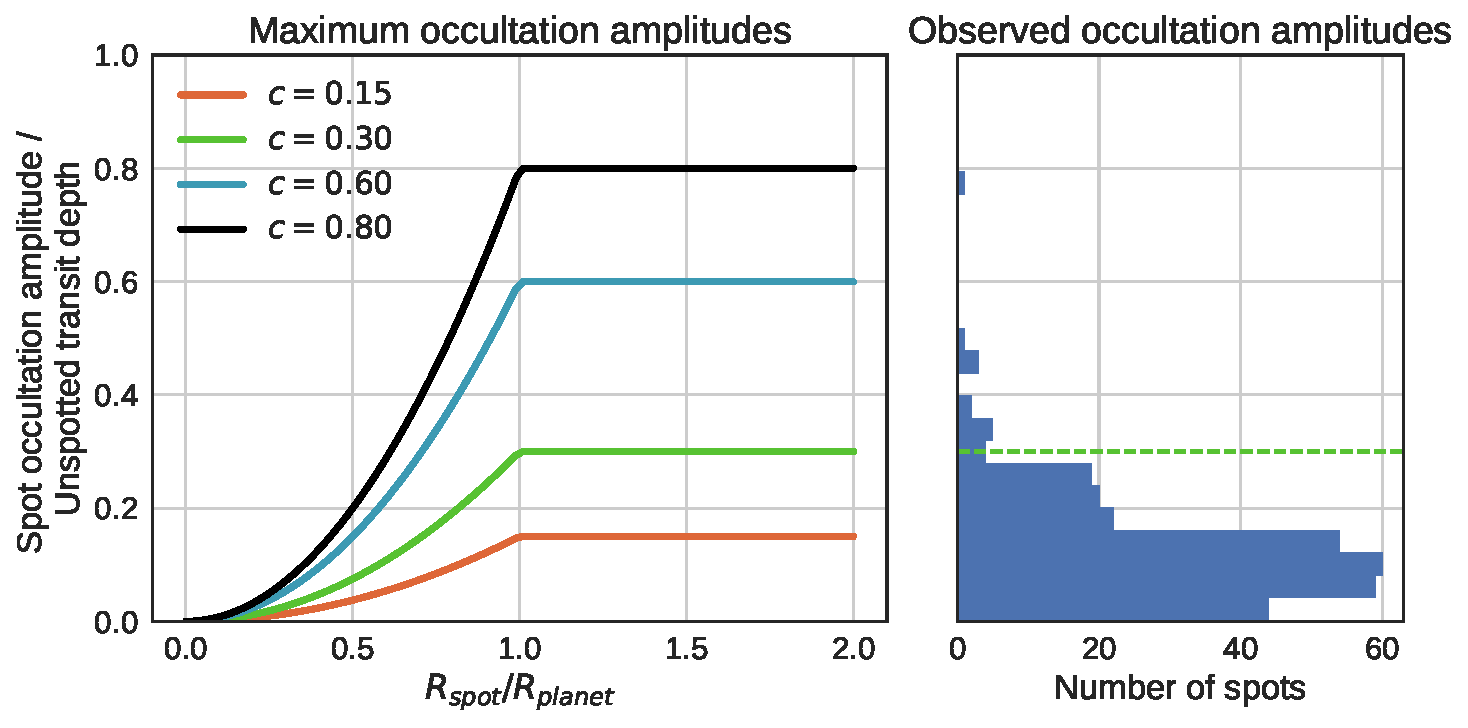
\includegraphics[scale=0.35]{stsp_hat_p_11/contrasts.pdf}
\caption{\textit{Left:} amplitudes of positive flux anomalies during spot occultations, normalized to the unspotted transit depth, as a function of the spot size and contrast. \textit{Right:} observed spot occultation amplitudes of HAT-P-11. 95\% of the spot occultations have normalized amplitudes $\le 0.3$ below the green dashed line, as one would expect from spots with the mean solar contrast $c=0.3$. The largest observed spot-occultation amplitude requires a spot contrast $c \ge 0.8$ -- similar to the spot contrast of sunspot umbra. Since most other spots are consistent with the mean solar spot contrast $c = 0.3$, we adopt the solar contrast value for the spots of HAT-P-11.}
\label{fig:contrast}
\end{figure}

In this work, \stsp\ approximates starspots as circular features with homogeneous contrast. We can define the spot intensity contrast relative to the local photosphere $c$ as
\begin{equation}
c = 1 - I_{spot}/I_{phot} \label{eqn:contrast}
\end{equation}
where $I_{spot}$ is the mean intensity inside the dark spot, $I_{phot}$ is the intensity of the local photosphere, and $I_{spot} < I_{phot}$. Spots with temperatures and intensities similar to the local photosphere $I_{spot} \approx I_{phot}$ are ``low contrast'', i.e. $c \rightarrow 0$, and spots with extreme temperature differences $I_{spot} \ll I_{phot}$ are ``high contrast'' and $c\rightarrow 1$. High-resolution studies of sunspots show that the spot darkness correlates with magnetic field strength in the vertical component \citep{Keppens1996, Leonard2008}.

Sunspots have complicated substructures each with their own contrast, such as the dark umbra and less dark penumbra. We cannot typically resolve such substructure in occultation photometry, so we chose to adopt the area-weighted contrast of the penumbra and umbra as the contrast for the entire spot. We can approximate sunspots as homogeneous circular features if we average over the penumbra and umbra, which have contrasts $c_{umbra} \sim 0.5 - 0.8$ and $c_{penumbra} \sim 0.15-0.25$. The mean area encompassed by the penumbra is roughly four times larger than the umbral area \citep{Solanki2003}. Adopting $c_{umbra} = 0.65$ and $c_{penumbra} = 0.2$, the area-weighted mean spot contrast of sunspots is $c_{total} = 0.3$. 

We can compare solar spot contrasts to constraints on the spot contrasts of HAT-P-11 from \kepler\ photometry. Spot contrasts are constrained by the amplitudes of spot occultations events. The difference in flux during a transit with a spot occultation and a transit without a spot occultation is set by the spot contrast, and the projected size of the spot compared to the planet. We derive spot occultation amplitudes as a function of spot radius and contrast in Appendix~\ref{sec:appendix_contrast}.

In Figure~\ref{fig:contrast} we compare the spot occultation amplitudes normalized by the flux of the unspotted star at each time during the transit, for a variety of spot contrasts and spot sizes with the observed spot amplitudes. As the spot contrast $c$ increases and the spot becomes darker, the amplitude of the spot occultation increases for spots of any radius. For spots larger than the planet, the contrast controls the maximum occultation amplitude. Therefore the maximum observed spot occultation amplitude sets a lower bound for the maximum spot contrast. The spot occultation with the largest normalized amplitude $\sim 0.80$ requires a spot contrast of $c_{min} \ge 0.8$, which is similar to the contrast of sunspot umbra. 95\% of the spot amplitudes could be produced by occultations of spots with the area-weighted mean solar spot contrast $c = 0.3$, so we adopt $c = 0.3$ as our spot contrast in fits with \stsp\ model, since it is consistent with both the spots of the Sun and HAT-P-11.

\section{Detailed \stsp\ Spot Occultation Model} \label{sec:stsp}

The \stsp\ model is constructed as follows \citep[see][for more details]{Hebb2017}. The star is represented by a series of discrete concentric circles with intensities decreasing radially outward to approximate limb darkening. Spots on the star are represented as non-overlapping circles that are darker than the local photosphere, which follow the stellar surface in fixed-body rotation. Each spot is defined by four parameters: radius, latitude, longitude, and intensity contrast relative to the photosphere. The planet is represented by an opaque circle, and the relative flux received by the observer is calculated throughout the orbit of the planet. We marginalize over the spot position and radius parameters.

We fit for spot properties with \stsp\ using the number of spots and initial positions given by the simple model in Section~\ref{sec:friedrich}, which narrows the sample to 138 transits with highly significant spot occultations. We approximate stellar limb darkening with 40 concentric circles. We fix the spot contrast to $c=0.3$, which we justified in Section~\ref{sec:contrast}.

We run the affine-invariant MCMC with 300 chains and no priors for each transit, until the parameter posterior distributions are stationary \citep{Goodman2010}. One advantage of the pure \texttt{C} implementation of \stsp\ is that it is naturally portable and scalable for distributed computing. We run \stsp\ for each of the 138 transits independently on the Extreme Science and Engineering Discovery Environment (XSEDE) Open Science Grid \citep{osg, xsede}. 


\subsection{Model parameter degeneracies}  \label{sec:degen}

\begin{figure}
\centering
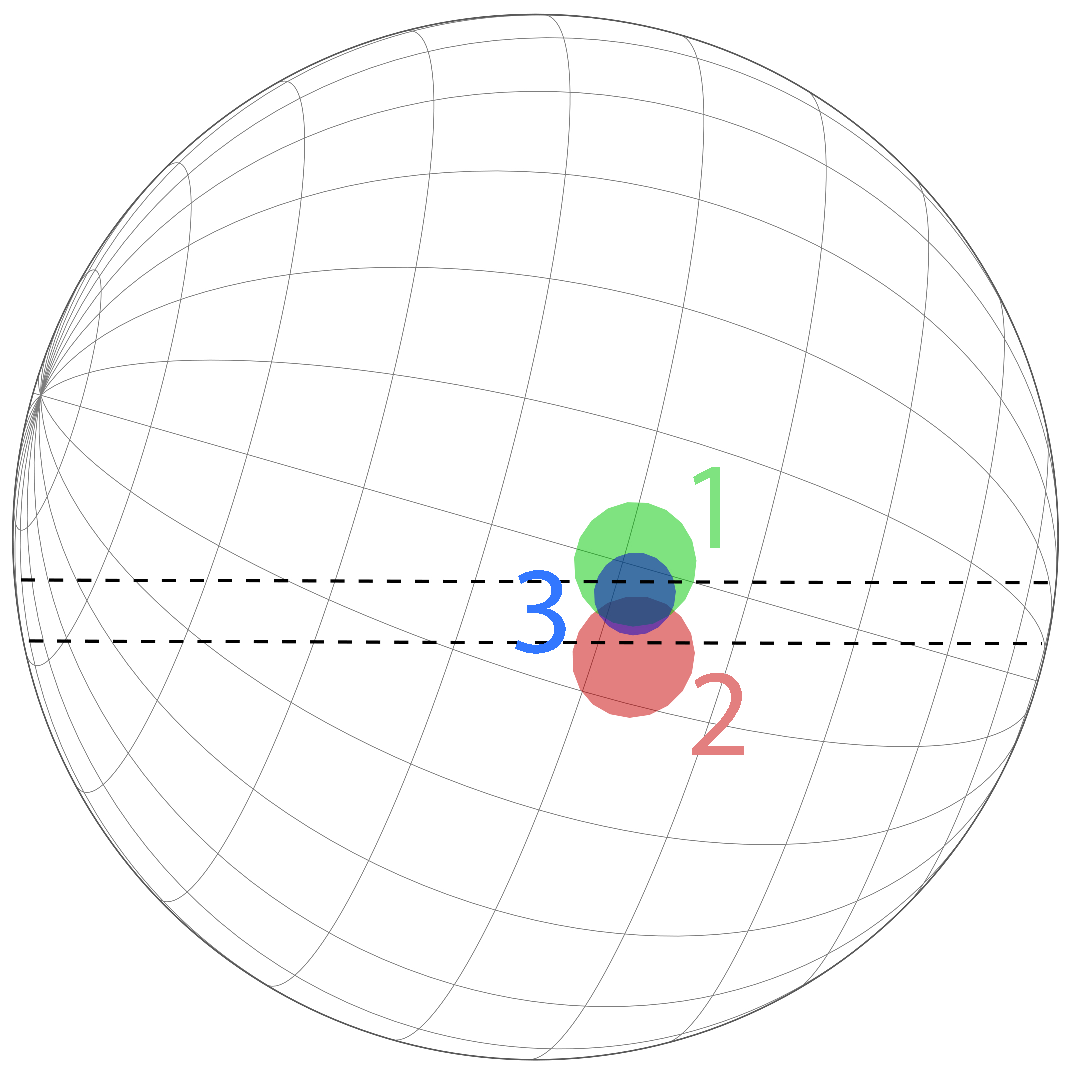
\includegraphics[scale=0.2]{stsp_hat_p_11/spot_degeneracy2.pdf}
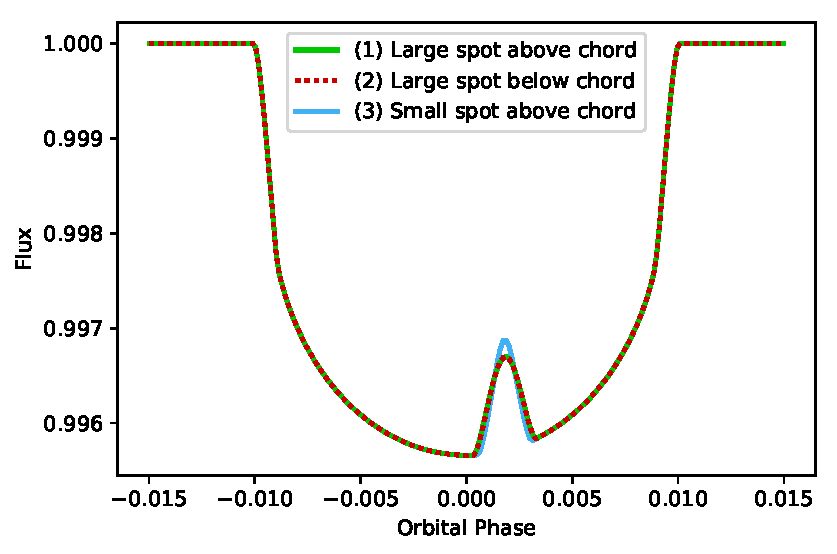
\includegraphics[scale=0.45]{stsp_hat_p_11/spot_degeneracy.pdf}
\caption{\textit{Upper}: Map of a few hypothetical spots on HAT-P-11 which would produce similar anomalies in the transit light curve.  The transit chord is bounded by the black dashed lines, the red latitudinal grid mark is the stellar equator -- the stellar rotational pole is tilted into the page and on the right. In this diagram, the planet transits from left to right, from near opposite the rotational pole to near the rotational pole. The ($R_{spot}/R_{star}$, latitude, longitude)  parameters for spot 1 (green), 2 (red), and 3 (blue) are: (0.12, 1.4$^\circ$, 359.8$^\circ$), (0.12, 4.3$^\circ$, 9.8$^\circ$), and (0.08, 2.3$^\circ$, 2.9$^\circ$), respectively. \textit{Lower:} \stsp\ model transits for each spot in the map above. With \kepler's flux precision for HAT-P-11 ($\sim 80$ ppm), these three models would be indistinguishable.}
\label{fig:rp_degeneracy}
\end{figure}

For most transit light curves with spot occultations, there exists a series of spot positions and radii which produce equally good fits to the observations. There are two main degeneracies in our choice of spot model which are critical to understanding the fit results of HAT-P-11; we will call these degeneracies: (1) the transit chord degeneracy and (2) the radius-position degeneracy. 

The transit chord degeneracy is a simple consequence of symmetry. For any small spot placed near the transit chord, a spot of the same radius could be placed on the opposite side of the transit chord (at the same distance from the transit chord) to create an identical bump in the light curve. See for example spots 1 and 2 in Figure~\ref{fig:rp_degeneracy}. 

The transit chord degeneracy may be broken in two scenarios: (1) for some star-planet systems with large impact parameters, the spots would be significantly more foreshortened on one side of the transit chord than the other; or (2) large spots that subtend large angles from the center of the stellar disk to the limb will be more foreshortened near the limb than at disk center, producing asymmetries between spot-crossing ingress and egress. HAT-P-11 has impact parameter $b = 0.141$ so spots projected onto either side of the transit chord will appear roughly symmetric, and therefore the spot position solutions most often come in pairs that are symmetric about the transit chord. However, there are a few exceptionally large spots that give rise to asymmetric spot crossings, which allows the model to select a spot position on only one side of the transit chord.

The radius-position degeneracy arises from trade-off in spot occultation amplitude between spot size and position. A large spot which grazes the edge of the transit chord will produce a bump in the transit light curve similar to a much smaller spot laying within the transit chord. See for example spots 1 and 3 in Figure~\ref{fig:rp_degeneracy}. 

The radius-position degeneracy can be broken with observations at infinite time resolution and flux precision. In the \kepler\ observations of HAT-P-11, the one minute cadence and the single measurement uncertainty $\sigma_{\Delta F / F} \sim 80$ ppm prevent us from distinguishing between small spots near to the transit chord and somewhat larger spots farther from the transit chord. 

More details about \stsp\ model parameter degeneracies are discussed in \citet{Hebb2017}. Examples of \stsp\ fits to the HAT-P-11 light curves and the effects of these degeneracies are discussed in detail in the following section.

\subsection{Examples of degeneracies in results}


\begin{figure}
\centering
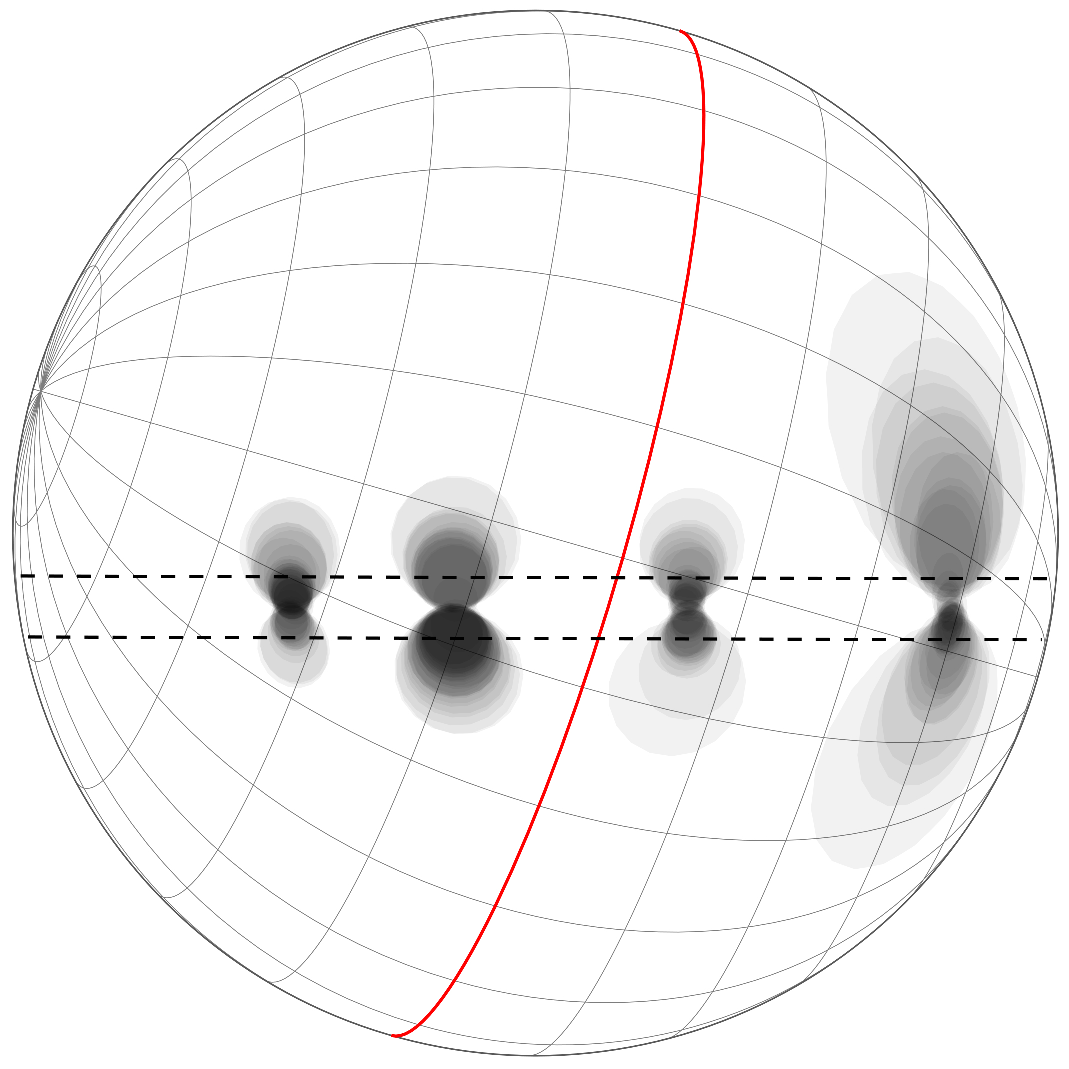
\includegraphics[scale=0.2]{stsp_hat_p_11/transit063.pdf}
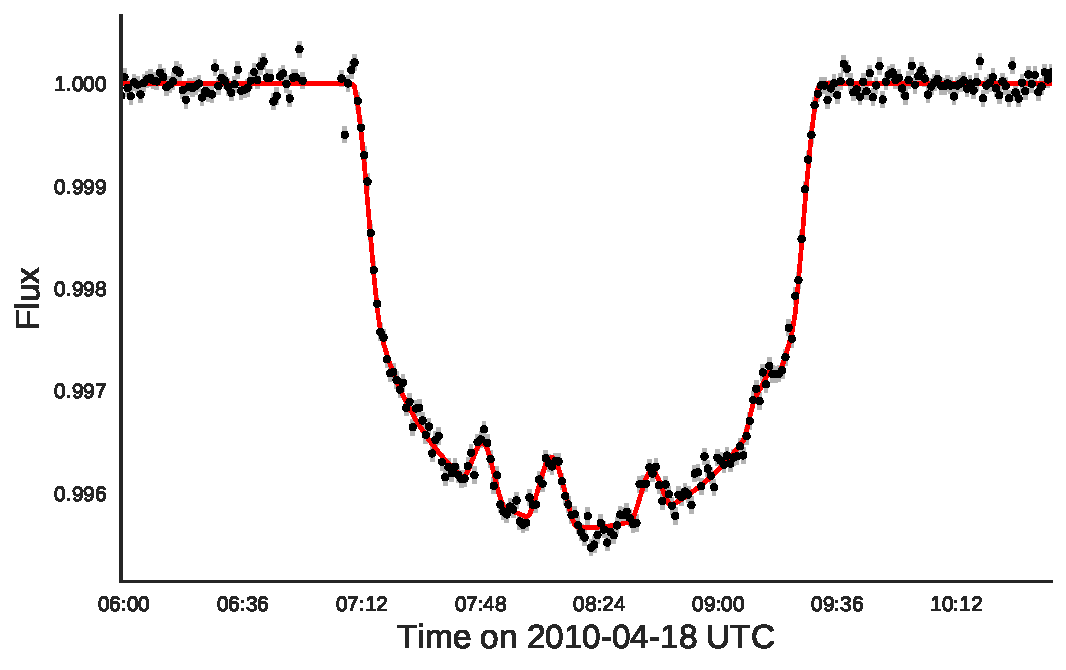
\includegraphics[scale=0.45]{stsp_hat_p_11/lc_063.pdf}
\caption{\textit{Lower:} an example transit light curve of HAT-P-11 b (black points) with the maximum likelihood \stsp\ model (red curve). \textit{Upper}: a few random draws from the posterior samples for the spot positions and radii. These four spots are highlighted in blue on the spot map in Figure~\ref{fig:map}.}
\label{fig:transit_063}
\end{figure}

\begin{figure}
\centering
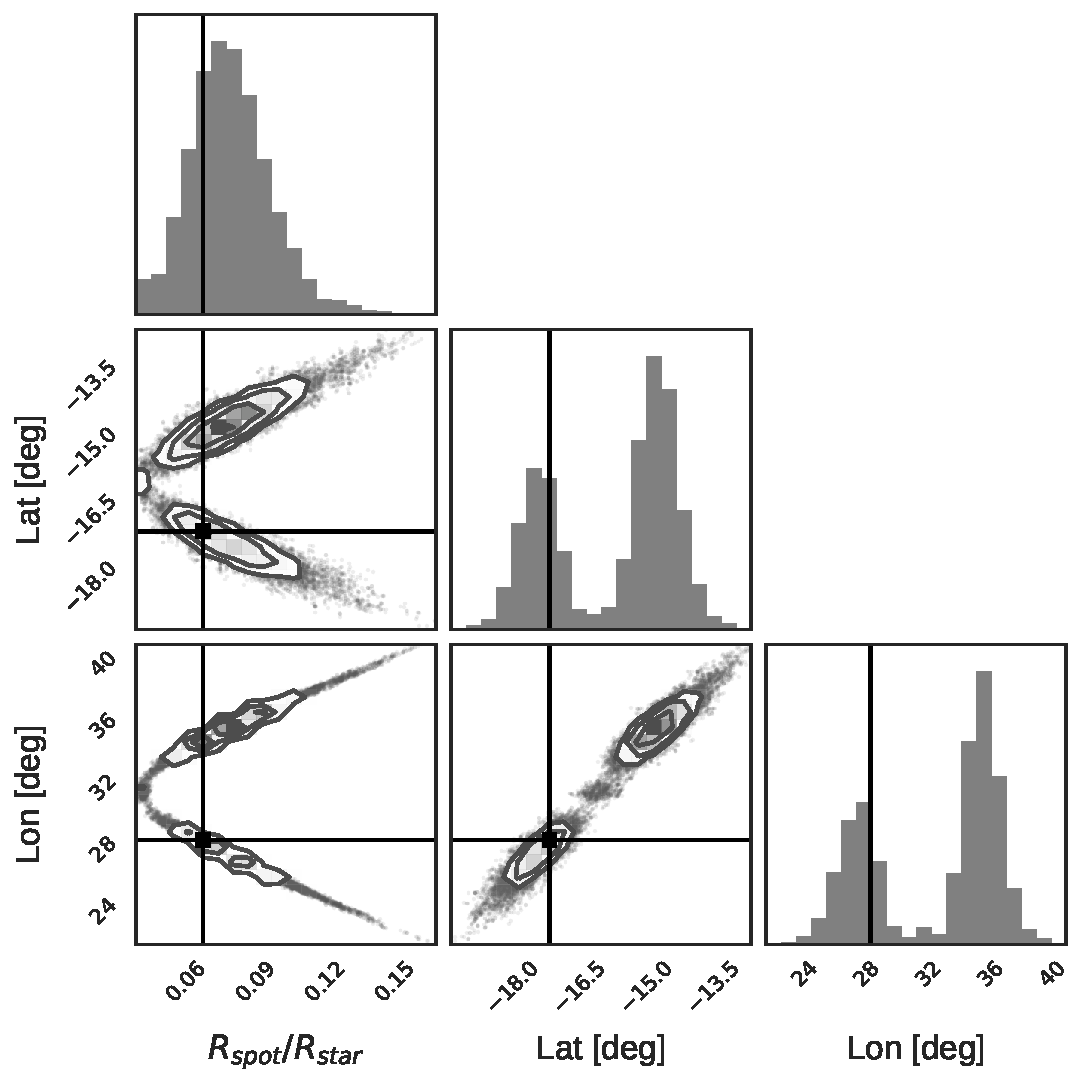
\includegraphics[scale=0.45]{stsp_hat_p_11/063_spot1_rll.pdf}
\caption{Correlations between posterior samples for latitude, longitude and spot radius for the spot second from the left in the graphic in Figure~\ref{fig:transit_063}. The vertical/horizontal black lines mark the maximum likelihood values from the Markov chains. For the analysis of the spot latitude and radius distributions, we use the maximum likelihood values to compute the spotted area in the transit chord, for example, which selects one of the two possible groups of solutions for each spot. Note that the model constrains the minimum spot radius for this spot despite the position-radius degeneracy, which is a result of fixing the spot contrast.}
\label{fig:corner_063}
\end{figure}

We can begin to understand the spot radius-position degeneracy which affects the radius distribution by inspecting the transit on April 18, 2010; see Figures~\ref{fig:transit_063}  and \ref{fig:corner_063}. There are four spot occultations visible in the transit light curve, so we seed the \stsp\ model with four spots, and optimize for the latitude, longitude and radius of each spot with fixed flux contrast ($c=0.3$, as defined in Equation~\ref{eqn:contrast}). The posterior samples for latitude, longitude and radius of each spot cluster into two groups of solutions -- one on each side of the transit chord. In some spot occultations, asymmetry in the photometry produces a preferred solution on one side of the transit chord. In the case of the spot posteriors shown in Figure~\ref{fig:corner_063} (see also the light curve and spot geometry in Figure~\ref{fig:transit_063}), the latitude and longitude have bimodal solutions. Therefore, rather than adopting the mean of these bimodal posteriors as the best solution, we use the parameter values at the maximum likelihood step of the MCMC chains to study spot radii (and latitudes).

For a fixed spot contrast, the radius-position degeneracy biases us towards larger radii. The asymmetry towards large radii can be seen in the bottom left plot of Figure~\ref{fig:corner_063}. If the spot contrast cannot vary, there exists a minimum spot radius which is capable of reproducing the observed occultation amplitude for a direct spot occultation (impact parameter $b=0$). Any indirect or grazing occultations ($b \neq 0$) would require a larger spot to produce the same occultation amplitude, producing an abundance of possible solutions with large spots, centered farther away from the transit chord. For this reason, we do not assert that any spots on HAT-P-11 are certainly larger than the largest sunspot, though the maximum likelihood solutions suggest such spots exist (more on spot radii in Section~\ref{sec:radii}).

\begin{figure}
\centering
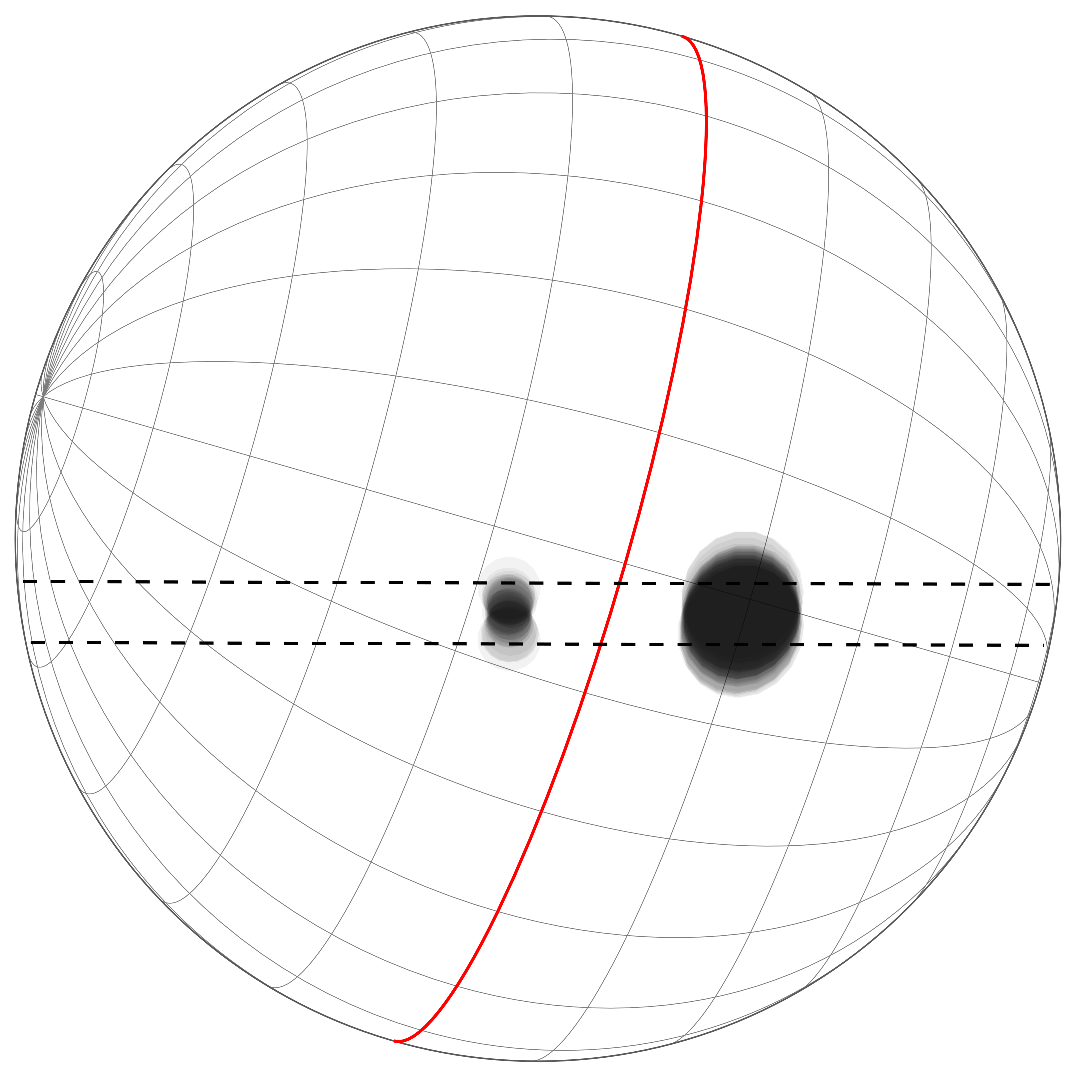
\includegraphics[scale=0.2]{stsp_hat_p_11/transit044.pdf}
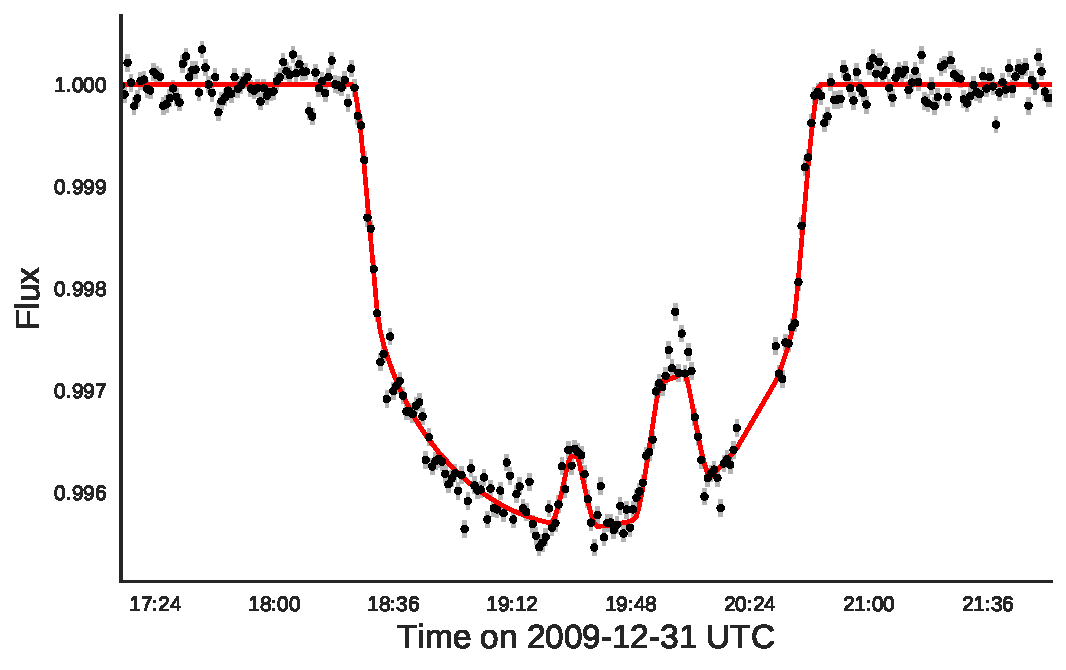
\includegraphics[scale=0.4]{stsp_hat_p_11/lc_044.pdf}
\caption{\textit{Lower:} an example transit light curve of HAT-P-11 b (black points) with the maximum likelihood \stsp\ model (red curve). \textit{Upper}: a few random draws from the posterior samples for the spot positions and radii. The transit chord is bounded by the black dashed lines, the red latitudinal grid mark is the stellar equator -- the stellar rotational pole is tilted into the page and on the right. In this diagram, the planet transits from left to right, from near opposite the rotational pole to near the rotational pole. The grid lines are separated by 15$^\circ$, so the active latitudes appear near the grid lines on either side of the equator. Note that the flat-topped spot occultation model light curve corresponds to a spot that must appear to be wider than the transit chord -- setting a constraint on the minimum radius of the spot. The observed fluxes are higher than the model near the mid-occultation time, which is suggestive of a higher spot contrast near the center of the spot. These two spots are highlighted in red on the spot map in Figure~\ref{fig:map}. In physical units, these spots have radii of $22400^{+4000}_{-300}$ and $63700^{+3000}_{-200}$ km.}
\label{fig:transit_044}
\end{figure}


Figure~\ref{fig:transit_044} shows an example light curve model and a few draws from the spot parameter posteriors for the transit on December 31, 2009 UTC. The model of the second spot occultation in this transit has a flat top, and an amplitude similar to $\Delta F/ \delta \sim c = 0.3$, which implies that the spot was occulted with a small impact parameter, and that the spot radius was larger than the planet radius. The geometry of this eclipse parallels planetary transits with negligible limb-darkening, which produce a ``u''-shaped eclipse with a flat bottom. We note that the \kepler\ fluxes at the peak of the second spot occultation have a net positive scatter. This could imply that a more extreme spot contrast is justified at the center of the spot ($c<0.3$), where one might expect the umbra to be. The duration of the flat-topped spot occultation is proportional to the diameter of the spot, so the position and size of this spot are relatively well-constrained by the photometry. This is reflected by the uniformity of the posterior samples of the second spot in Figure~\ref{fig:transit_044} compared to the earlier grazing spot occultation, which is less constrained. The inverted ``v''-shape of the first spot occultation implies that the planet either grazed the spot at high impact parameter -- similar to planetary transits or binary eclipses with high impact parameters, which produce ``v''-shaped eclipses -- or that the spot is similar in size to the size of the planet. As you can see in the samples from the posteriors on the map in Figure~ \ref{fig:transit_044}, the model tends towards a spot centered in the transit chord, slightly smaller than the planet. 



\section{\stsp\ Results} \label{sec:results}
\subsection{Spot Map of HAT-P-11}

\begin{figure*}
\centering
% \includegraphics[scale=0.3]{map_friedrich.pdf}
%\includegraphics[scale=0.58]{map_stsp.pdf}
\includegraphics[scale=0.58]{stsp_hat_p_11/map_stsp.pdf}
\caption{Spots detected on HAT-P-11 with \stsp\ (see Section~\ref{sec:stsp}). The radius of each circle corresponds to the size of the spot. The shading beneath corresponds to the number of times the planet occulted that spatial bin on the stellar surface, which can be used as a proxy for relative completeness. Note that the spots occur preferentially at two active latitudes near $\pm15^\circ$. The 6:1 period commensurability between the orbital period and stellar rotation period produces the alternating longitudinal stripes in relative occultation number. The two red circles in the western hemisphere near longitude $-90^\circ$ highlight the spots derived from the transit light curve in Figure~\ref{fig:transit_044}, and the four blue circles in the eastern hemisphere near longitude $30^\circ$ correspond to the spots derived from the transit light curve in Figure~\ref{fig:transit_063}. The green circle near longitude $-100^\circ$ corresponds to the large spot discussed in Figure~\ref{fig:transit_071}.}
\label{fig:map}
\end{figure*}

We map the maximum-likelihood starspot positions for all 138 transits in Figure~\ref{fig:map}. The circles represent the positions and sizes of the spots inferred with \stsp. The shading of the map corresponds to the number of times the center of the planet occulted each location on the star, which is a proxy for completeness of the spot map -- darker regions were occulted more often. We choose to plot the maximum-likelihood spot positions and radii rather than the means of the posterior samples, because degeneracies between the model parameters can produce bimodal posterior distributions (see Section~\ref{sec:stsp} for discussion on model degeneracies).

The spin-orbit misalignment and spin-orbit commensurability of this system lead to highly inhomogeneous sampling in longitude, so an investigation into the true spot longitude distribution is beyond the scope of this work. However, asymmetries in spot latitude are detectible and readily visible in the spot map in Figure~\ref{fig:map}. The spots are distributed into two active latitudes near $\pm 16^\circ$ latitude, and the northern hemisphere appears to have more spots than the southern hemisphere. We investigate the latitude distribution of spots in the next section.

The transit chord of HAT-P-11 b is inclined $16^\circ$ from perpendicular to the stellar equator -- refer back to Figure~\ref{fig:schematic} for a schematic of the orientation. As a result of this slight misalignment from perpendicular, the planet never occults either pole of the star. It is possible that there are spots at latitudes $\ge 60^\circ$, which have been produced in simulations of highly-active sun-like stars \citep[e.g.][]{Schrijver2001}. Our spot map from transit photometry is insensitive to polar or high latitude spots. 

\subsection{Latitude Distribution} \label{sec:lat_dist}

\begin{figure}
\centering
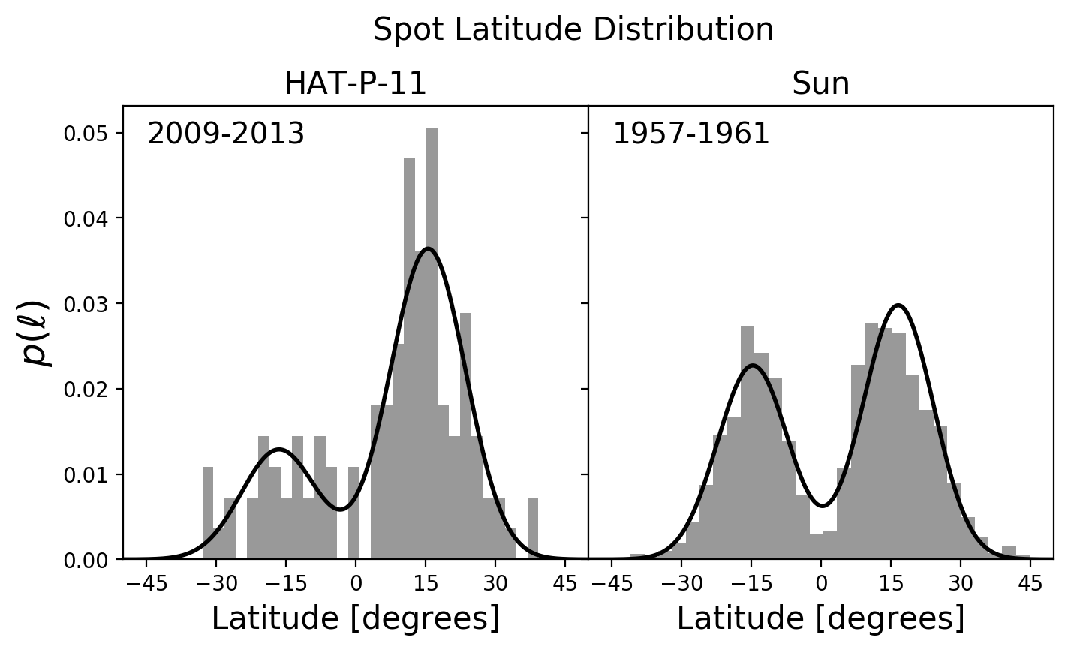
\includegraphics[scale=0.48]{stsp_hat_p_11/asymmetric_latitudes.pdf}
\caption{Distribution of spot latitudes over four years of observations for both HAT-P-11 and the Sun. The four years of solar observations correspond to the maximum of solar Cycle 19 as observed by \citet{Howard1984}. The HAT-P-11 spot latitudes and their uncertainties are taken from the best-fit solutions from the \stsp\ spot occultation model. Both stars have active latitudes centered on $\pm 16^\circ$ with standard deviations of $\sim 8^\circ$. We put these latitude distributions in context throughout the solar activity cycle in Figure~\ref{fig:sun_vs_hat11}. Though HAT-P-11's hemispheric spot number asymmetry is greater than the Sun's in this particular bin of solar observations, we find that the asymmetry on HAT-P-11 is within the range observed on the Sun; see Section~\ref{sec:lat_dist} for details.}
\label{fig:latitude_model}
\end{figure}

\begin{figure}
\centering
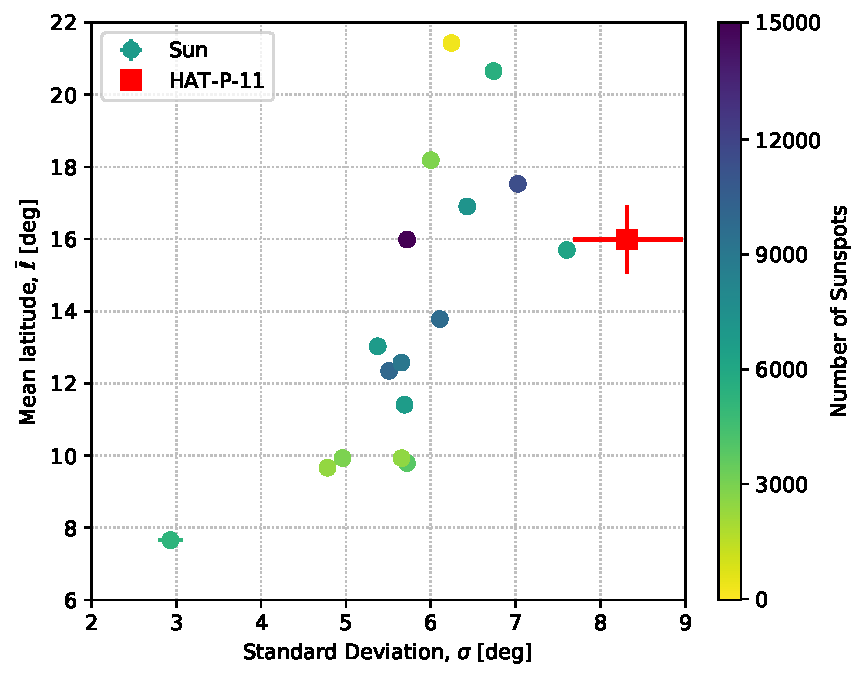
\includegraphics[scale=0.6]{stsp_hat_p_11/sun_vs_hat11.pdf}
\caption{Latitude distributions of sunspots and spots on HAT-P-11, parameterized by the mean latitude of spots in each hemisphere and the standard deviation of spot latitudes in each hemisphere. The circles are the best-fit parameters for four-year bins of the Mt.~Wilson sunspot catalog \citep{Howard1984}. The squares are fits to the HAT-P-11 latitude distribution over the four years of \kepler\ data. The colors of the solar circles represent the number of sunspots in each bin, which is a good proxy for phase of the solar activity cycle (darker points are nearer to solar maximum). Some of the fits have large uncertainties even with many spots, because the latitude distributions are not always well-approximated by Gaussians. The solar measurement closest to HAT-P-11's corresponds to the period 1957-1961 during solar Cycle 19, which is plotted in Figure~\ref{fig:latitude_model} for comparison to HAT-P-11.}
\label{fig:sun_vs_hat11}
\end{figure}

The mean latitudes of sunspots and the widths of their distributions across each hemisphere undergo an $\sim 11$ year cycle, which gives rise to the ``butterfly diagram'' of latitudinal spot density as a function of time \citep[see for example][]{Hathaway2011, Hathaway2015}. Near solar minimum, there are very few sunspots. Spots begin to appear at ``high'' latitudes $\left | \ell \right |  \sim 25^\circ$, and the mean spot latitude drifts towards the equator throughout the cycle, with the maximum number of spots occurring near $\left | \ell \right | \sim 15^\circ$. The northern and southern hemispheres of the Sun can have asymmetric numbers of spots, flares, and other activity indicators \citep[see for example][]{Newton1955, Vizoso1990, Carbonell1993, Li2002}.

To compare the activity of HAT-P-11 to solar activity, we characterize the Sun's spot latitude distribution in the 1917-1985 sunspot catalog from Mt.~Wilson Observatory published by \citet{Howard1984}. We group the solar spot observations into four-year bins similar to the \kepler\ time series of HAT-P-11. On these timescales, the spot latitude distributions on both stars are often similar to Gaussians (see Figure~\ref{fig:latitude_model}), though sometimes the deviations from Gaussians are significant.

We construct a probabilistic model to describe the latitude distributions of spots on HAT-P-11 and on the Sun, following the description of the Gaussian mixture model in Section~\ref{sec:i_s}. We fit for the amplitude, mean, and variance of Gaussians representing the latitude distributions of spots in each hemisphere. We focus on fitting the shape of the latitude distribution and do not compare the total number of spots observed on the two stars to each other, since a correction for the sensitivities and biases of the different observing methods is beyond the scope of this paper.

The latitude distribution of spots of HAT-P-11 and four years of solar observations are shown in Figure~\ref{fig:latitude_model}. The four-year span of solar observations closely resembles the mean spot latitudes and standard deviation of spot latitudes that we measure for HAT-P-11. The sunspots included in Figure~\ref{fig:latitude_model} span the active maximum of solar Cycle 19, which was the solar maximum with the largest recorded number of spots since telescopic observations began \citep{Solanki2013}.

The properties of the maximum-likelihood Gaussian mixture models for HAT-P-11 and the Sun are shown in Figure~\ref{fig:sun_vs_hat11}. The circles show the mean latitudes of spots on each hemisphere of the Sun, and the standard deviations of the spot distributions. The pattern of the solar activity cycle is visible --- sunspots in the beginning of the cycle appear in small numbers at high latitudes, then large numbers near $15^\circ$, before settling back to lower numbers near the equator. The standard deviations of the spot distributions are correlated with the mean latitude --- the active latitudes are broadest at the beginning of the activity cycle when spots form at high latitudes, and the active latitudes become narrower as they approach the equator later in the activity cycle. The combined effect of the shrinking standard deviations with declining mean latitudes produces the ``wings'' in the butterfly diagram.

The distribution of spots on HAT-P-11 sits near the region of $\bar{\ell} - \sigma$ space corresponding to solar maximum. The most similar four-year bin of sunspots, which is roughly consistent with the HAT-P-11 spot distribution in terms of $\bar{\ell}$ and $\bar{\sigma}$, is the bin plotted in Figure~\ref{fig:latitude_model}. The mean active latitudes on HAT-P-11, $\ell = 16 \pm 1^\circ$, correponds to the mean latitudes of sunspots near most solar maxima.

The number of spots observed in each hemisphere is rather asymmetric, but within the range of observed asymmetries on the Sun. Hemispheric asymmetries of the solar spot distribution are often quantified by $(N-S)/(N+S)$, where $N$ is the spot area in the northern hemisphere and $S$ is the spot area in the southern hemisphere \citep{Waldmeier1971, Carbonell1993}. The maximum likelihood \stsp\ spot latitudes and radii from the entire \kepler\ mission give $(N-S)/(N+S)=0.35$. This asymmetry is within the range observed on the Sun by \citet{Howard1984} when observed in four-year bins, varying from -0.1 to 0.6.

\subsection{Radius distribution} \label{sec:radii}

\begin{figure*}
\centering
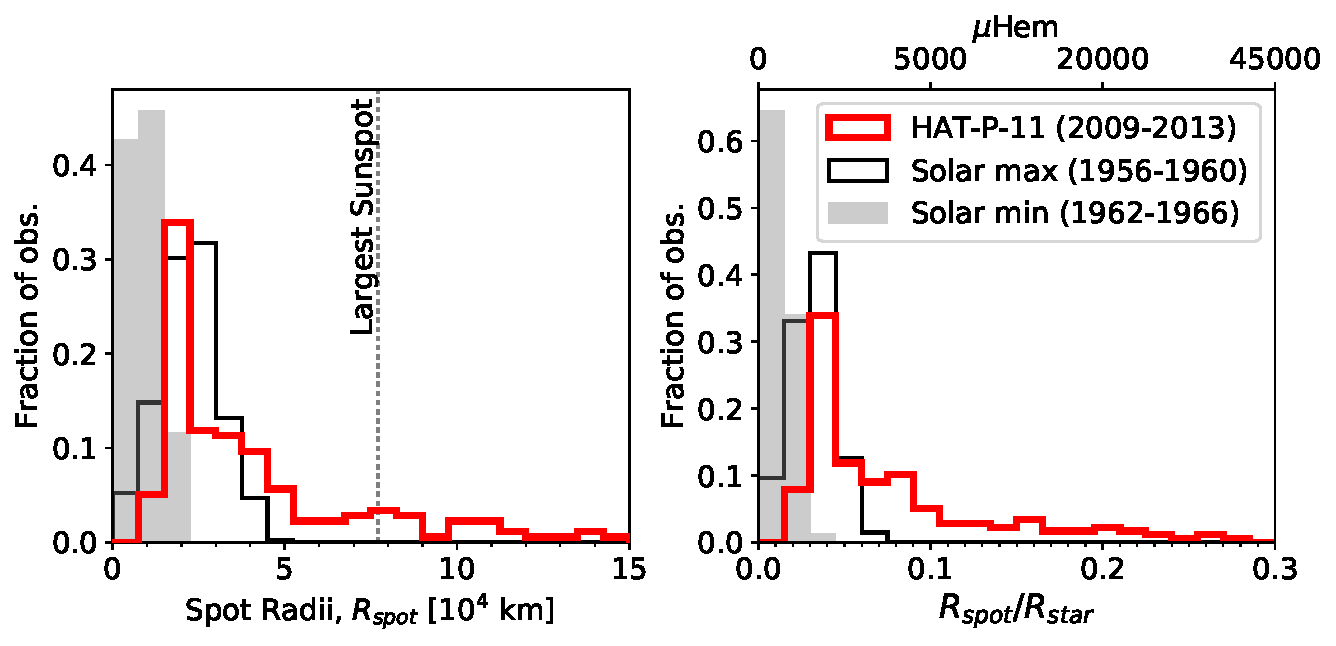
\includegraphics[scale=0.75]{stsp_hat_p_11/spot_radii.pdf}
\caption{Maximum likelihood spot radii for HAT-P-11 from \kepler\ spot occultations, and for the Sun from Mt.~Wilson Observatory \citep{Howard1984}. The spot radii are given in physical units on the left panel and in fractions of the stellar radius ($R_{spot}/R_{star}$) and millionths of the observer-facing hemisphere ($\mu$Hem) in the right panel. We adopt the radius of HAT-P-11 from \citet{Bakos2010}, $R_{star} = 0.752 R_\odot$. For reference, the largest sunspot measurement we could find in the literature was 6132 $\mu$Hem = $R_{spot} / R_{\odot} = 7.7 \times 10^4$ km. We suspect that a significant fraction of HAT-P-11's spots with very large radii are in fact occultations of multiple spots.}
\label{fig:radii}
\end{figure*}

\begin{figure}
\centering
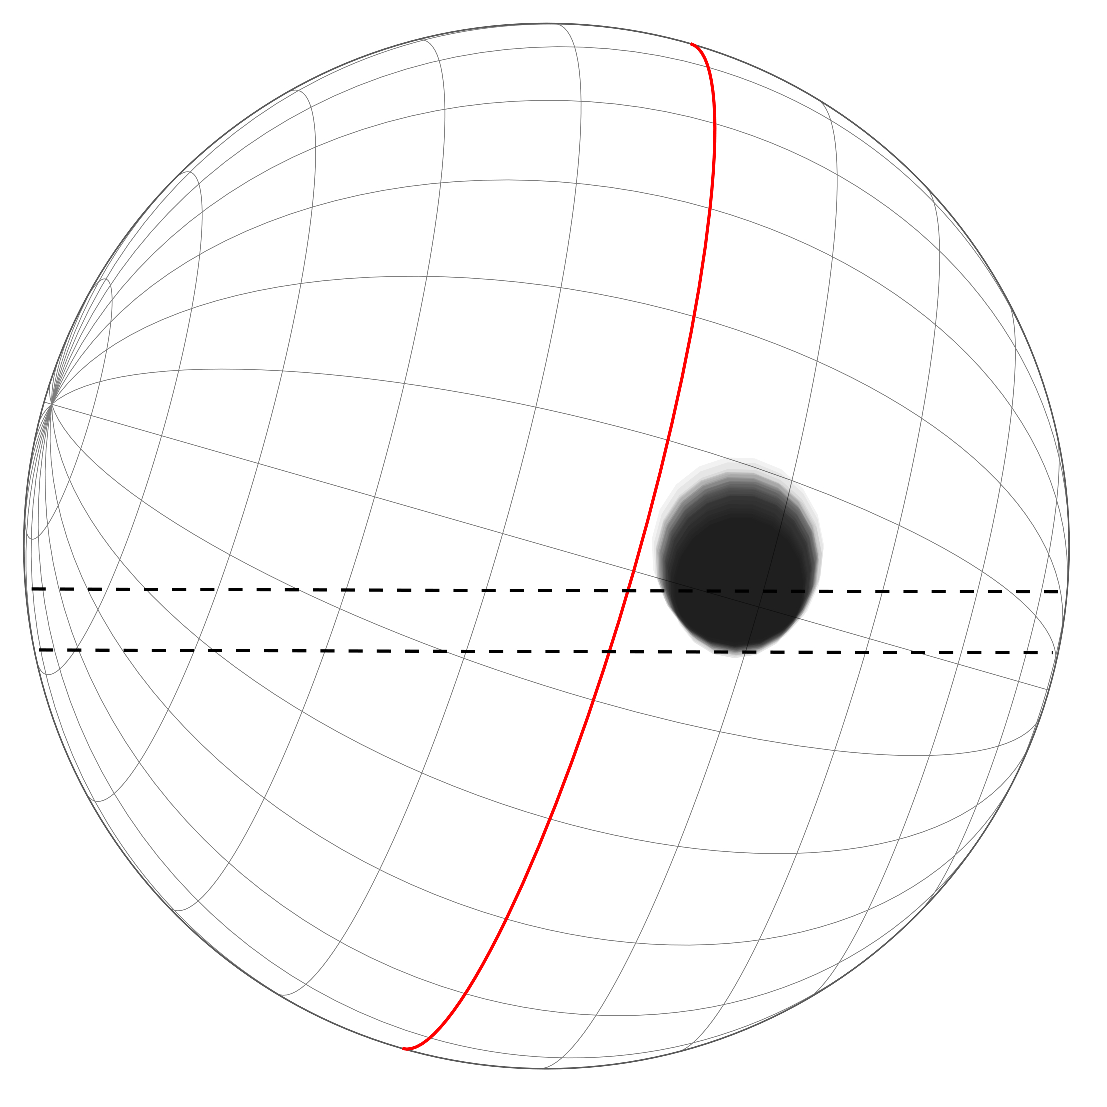
\includegraphics[scale=0.18]{stsp_hat_p_11/transit071.pdf}
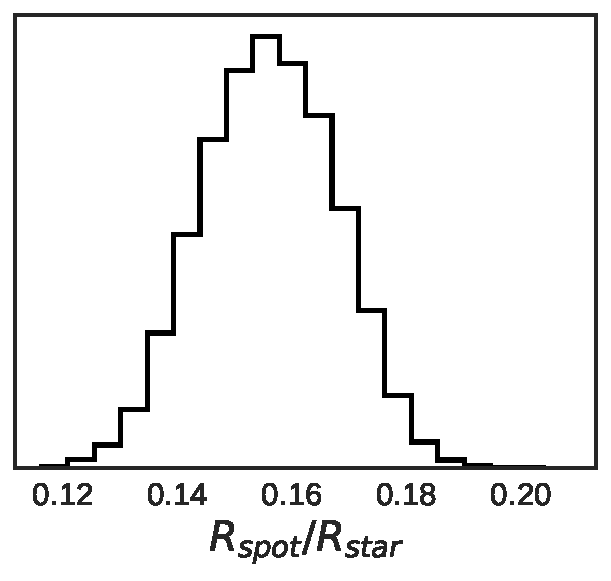
\includegraphics[scale=0.35]{stsp_hat_p_11/rad_071.pdf}
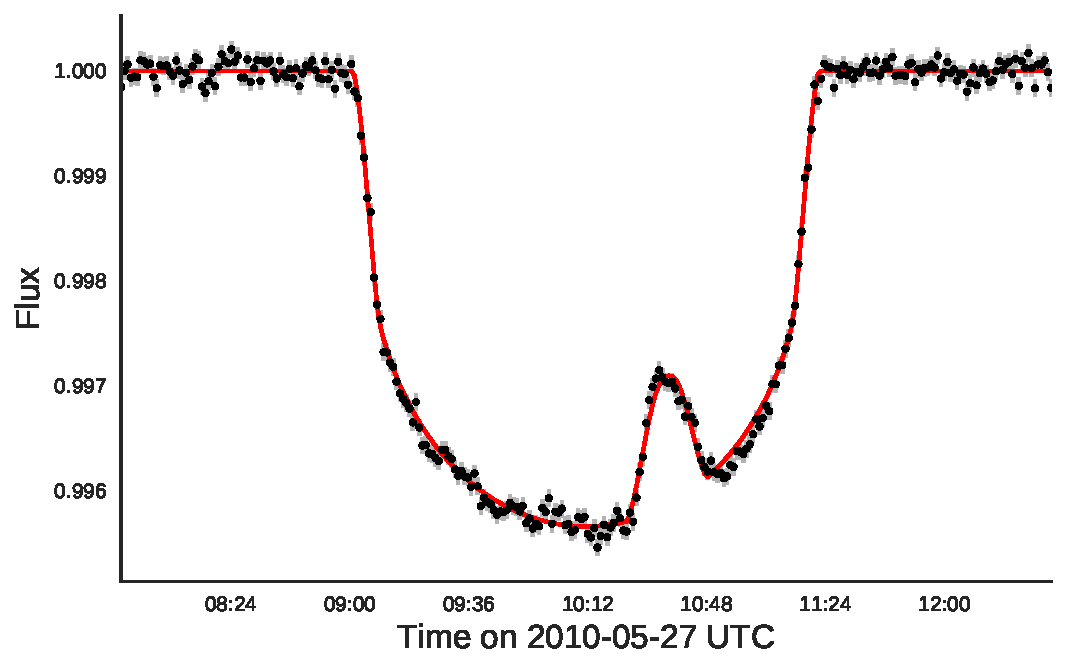
\includegraphics[scale=0.45]{stsp_hat_p_11/lc_071.pdf}
\caption{An occultation of a particularly large spot. The maximum likelihood spot radius is $R_{spot}/R_{star} = 0.160_{-0.016}^{+0.007}$, or $84000^{+4000}_{-8000}\pm 6000$ km -- just larger than the largest recorded sunspot (77000 km, \citealt{Newton1955}). This spot is highlighted in green on the spot map in Figure~\ref{fig:map}.}
\label{fig:transit_071}
\end{figure}

We compute the physical spot radius distribution using the radius measurement of HAT-P-11 from \citet{Bakos2010}, $R=0.752 \pm 0.021 R_\odot$. The spot radius distribution is shown in Figure~\ref{fig:radii}, along with sunspot radii near activity maximum and minimum. 

The spot radius distribution of HAT-P-11 closely resembles the Sun's at activity maximum for spots with radii $2\times 10^4 < R_{spot} < 5 \times 10^4$ km. 85\% of the spots on HAT-P-11 are smaller than the largest observed sunspot. The HAT-P-11 radius distribution is incomplete for small spots with $R_{spot} \lesssim 2 \times 10^4$ km, since spot occultation amplitudes of those spots are similar in scale to the noise in \kepler\ photometry. The smallest observed sunspots have radii of order $10^3$ km \citep{Solanki2003}, so it is likely that there are also small spots on HAT-P-11 below our S/N threshold.

HAT-P-11's spot distribution has a tail of spots larger than those observed on the Sun, with $R_{spot} > 5 \times 10^4$ km. From visually inspecting the individual transits, it is clear that some of the spots are larger than the largest sunspots. The largest published sunspot measurement that we encountered in the literature was recorded in 1947 by \citet{Newton1955} to have area 6132 $\mu$Hem. We can calculate the radius of a circular spot with this area in units of hemispheres (Hem) by normalizing the area of the circular spot $A_{spot} = \pi R_{spot}^2$ by the area of the observer-facing hemisphere of the star $A_{star} = 2\pi R_{star}^2$,
\begin{equation}
A_{\textrm{Hem}} = \frac{1}{2}\left(\frac{R_{spot}}{R_{star}}\right)^2\\ \\
\frac{R_{spot}}{R_{star}} = \sqrt{2 A_{\textrm{Hem}}}
\end{equation}
Therefore in the circular approximation, the largest reported sunspot had radius $R_{spot}/R_{\odot} = 0.110$ and $R_{spot} \sim 77$ Mm. We can compare that to the spot in Figure~\ref{fig:transit_071}, for example, which has $R_{spot}/R_{star} = 0.160_{-0.016}^{+0.007}$ corresponding to $R_{spot} = 84^{+4}_{-8}$ Mm --- consistent with the largest sunspot. The radius posterior distribution shown in Figure~\ref{fig:transit_071} has a single solution. However, many of these larger spots could be somewhat smaller than the maximum likelihood solution that we are reporting. The spot radius posterior distributions exhibit families of degenerate solutions in which the spot occultation fluxes can be fit equally well by a grazing spot occultation of a large spot or a more direct occultation of a smaller spot (see Section~\ref{sec:degen} for discussion of degeneracies). This could produce a systematic bias towards larger maximum-likelihood spot radii in the values that we report.


\subsection{Spotted area} \label{sec:spotted_area}

\begin{figure}
\centering
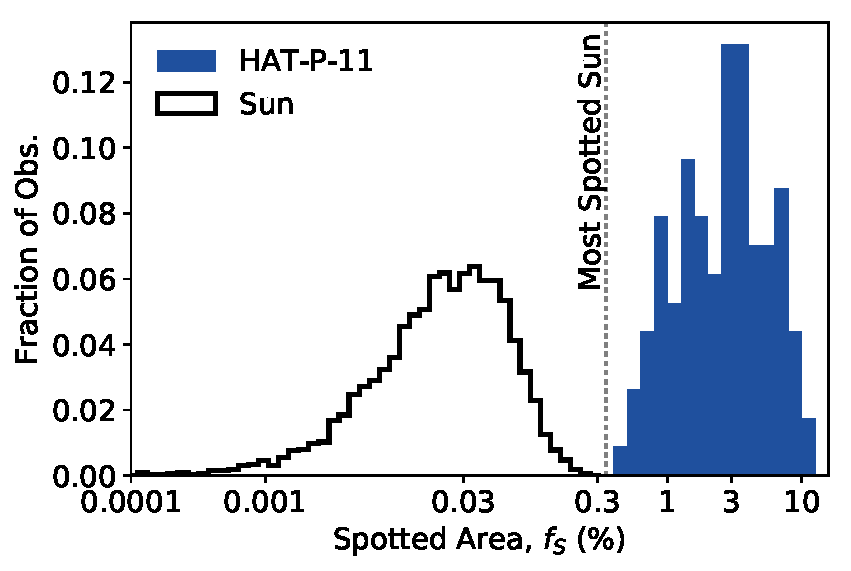
\includegraphics[scale=0.6]{stsp_hat_p_11/spotted_area.pdf}
\caption{Spot coverages of HAT-P-11 and the Sun. The HAT-P-11 spotted area is computed the area of the transit chord occulted by spots in the maximum likelihood \stsp\ fit. The spotted areas of the Sun are gathered from the Mt.~Wilson Observatory spot catalog of \citet{Howard1984}, scaled up to account for the areas of penumbra and penumbra, assuming an area ratio of $A_{pen} / A_{umb} = 4$. We have excluded spot coverages for transits that had either no significant spot occultations, or where multiple spot occultations were fit with a single unrealistically large spot, narrowing the sample down to 90 of the 205 transits observed by \kepler.}
\label{fig:spotted_area}
\end{figure}

\begin{table*}
\centering
\footnotesize
\begin{tabular}{|lccccccc|} 
\hline
Name & Sp. Type & $T_{eff}$ [K] & $P_{rot}$ [d] & $T_{spot}$ [K] & $f_s \, [A_{*/2}]$ & $\left < S \right>$ & Ref. \\ \hline \hline
Sun & G2V & 5777 & 24.47 & 3900-5500 & $0.0003^{+0.0006}_{-0.0001}$ & 0.17 & [1, 2, 3]\\
HAT-P-11 & K4V & 4780 & 29.2 & 4500 (fixed) & $3^{+0.06}_{-0.01}$ & 0.6 & (This work, [4]) \\
OU Gem  & K3V/K5V & 4925/4550 & 6.991848 & --- & $\le 0.04 - 0.35$ & 0.796 & [5, 6] \\
EQ Vir  & K5Ve & 4380 & 3.96 &  $3350 \pm 115$ &$0.33 - 0.45$ & 3.68 & [5, 7] \\
XX Tri & K0 III & 4750 & 23.96924 & $3425 \pm 120$ & $0.31 - 0.35$ & -- & [8] \\
V833 Tau & K4V & 4500 & 1.7955 & 3175  & 0.51 & 2.460 & [6, 8] \\ \hline
\end{tabular}
\caption{Comparison of HAT-P-11, the Sun, and several stars in order of increasing spot coverags ($f_S$, in units of hemispheres [$A_{*/2}$]). The spot temperature range listed for the Sun includes the typical lower limit of umbral temperatures and typical upper limit of penumbral temperatures. The spot temperature of HAT-P-11 is estimated by selecting the PHOENIX model atmosphere that most closely produces a spot contrast of $c=0.3$ in the \kepler\ bandpass \citep{Husser2013}, and should be thought of as the approximate area-weighted spot group temperature in both the umbra and penumbra. The typical solar spot temperature range spans from the coolest regions of the umbra to the hottest regions of the penumbra. References: [1] \citet{Howard1984}, [2] \citet{Solanki2003}, [3] \citet{Egeland2017}, [4] \citet{Bakos2010}, [5] \citet{ONeal2001}, [6] \citet{Pace2013}, [7] \citet{Cincunegui2007}, [8] \citet{ONeal2004},  }
\label{tab:fillfactors}
\end{table*}

The spot area coverage of the observable hemisphere of a star, or the spot ``filling factor'' $f_S$, has been constrained for several stars with Zeeman-Doppler imaging and molecular band modeling. Since these methods are sensitive to different spot sizes \citep{Solanki2004}, we chose to compare the spots that we detect on HAT-P-11 via photometry with starspots detected via molecular band modeling only. The molecular absorption band spot temperatures and filling factors from \citet{ONeal2001, ONeal2004} are enumerated in Table~\ref{tab:fillfactors}, with spot areas ranging from a few percent to nearly half of the stellar surface. 

We can calculate the spotted area within the transit chord at the maximum-likelihood step in the MCMC chains for each transit. This spotted area measurement is not identical to the spotted area fraction $f_S$ from \citet{ONeal2001, ONeal2004}, which measures the fractional area of spots on the entire observer-facing hemisphere of a star. However, since the transit chord of HAT-P-11 b is nearly perpendicular to the stellar equator, the planet occults most latitudes of the star at one longitude during each transit. Since we expect the distribution of starspots to be azimuthally symmetric -- i.e.~the spot distribution may change as a function of latitude but not longitude -- each transit samples the spotted area of a relatively unbiased slice of the stellar surface. Thus we use the spot coverage within the transit chord as a characteristic spot coverage on the whole star.

In Figure~\ref{fig:spotted_area}, we plot the spotted area within the transit chord for the 138 transits with significant spots modeled by \stsp, compared with the spotted area on the Sun (including both the umbra and penumbra). During the \kepler\ mission, the spotted area on HAT-P-11 varied with mean area coverage $\left< f_{s,H11} \right> = 3^{+6}_{-1} \%$, where the upper and lower error bars are the $84^\textsuperscript{th}$ and $16^\textsuperscript{th}$ percentiles, respectively. We have excluded the transits with no significant spot detections from the above reported $\left< f_{s,H11} \right>$ since the abundance of non-detections is distinct from measurements of zero spotted area; and as we discuss in Section~\ref{sec:spot_number}, the star likely always has large spots facing the observer.

The mode of the solar spot coverage from \citet{Howard1984} is $\left< f_{s,\odot} \right> = 0.0003^{+0.0006}_{-0.0001}$, $\sim$100x smaller than HAT-P-11's. Upper limits on the maximal recorded spotted area of the Sun vary depending on the observations considered, but are typically $\lesssim 0.6\%$ \citep{Balmaceda2009}.

We note that the completeness of spot detections on the Sun is nearly 100\%, whereas on HAT-P-11 we are only sensitive to large spots in the transit chord, which covers about 6\% of the observer-facing hemisphere. Therefore the spot coverage that we report for HAT-P-11 is best treated as a lower limit on the actual spot coverage. With that caveat in mind, HAT-P-11's spot coverage is most similar to the molecular band observations of OU Gem, which varies in the range $f_s \le 0.04$ to $0.35$ \citep{ONeal2001}. 

The high spot coverage of HAT-P-11 compared to the Sun is consistent with its CaII H \& K emission. The Sun's mean $S$-index during Cycle 23 was $\left<S_\odot\right> = 0.1701 \pm 0.0005$ \citep{Egeland2017}, compared to $\left<S_{H11}\right> = 0.61$ for HAT-P-11 \citep{Bakos2010}. The solar $S$-index directly correlates with the area coverage by sunspots, so naturally it follows from the high $S$-index that HAT-P-11 should have a higher spot coverage. 

\citet{Shapiro2014} fit for the the relation between sunspot coverage $f_{s,\odot}$ as a function of the solar $S$-index and found:
\begin{equation}
f_{s,\odot}(S) = 0.105 - 1.315 S + 4.102 S^2. \label{eqn:naive}
\end{equation}
If we naively substitute our measured spot coverage $f_{s,H11} \sim 0.03$ for HAT-P-11 into Equation~\ref{eqn:naive}, we predict $\left<S_{H11, pred}\right> \sim 0.26$. The observed $S$-index is much larger --- evidently the activity of Sun-like stars does not scale quadratically with $S$-index in the activity regime relevant to HAT-P-11.

We now revisit the assumption made in Section~\ref{sec:norm} that the maximum flux during each \kepler\ quarter is approximately the unspotted brightness of the star. The spotted area observed on HAT-P-11 is as high as 10\% at times, so the maximum quarterly flux is unlikely to be the unspotted flux of the star. If we are underestimating the unspotted flux of the star, then we will underestimate the transit depth (see Section~\ref{sec:norm}), and therefore underestimate spot occultation amplitudes. This propagates into underestimates of spot radii and underestimates of the spotted area. This bias acts to oppose the bias towards larger spot radii and larger spotted areas discussed in Section~\ref{sec:radii}. Visual inspection of the transit light curve residuals shows that the transit depth is generally consistent with the observations, so we deem that our normalization in Section~\ref{sec:norm} is sufficient.

\subsubsection{Spotted area via flux deficit}

\begin{figure}
\centering
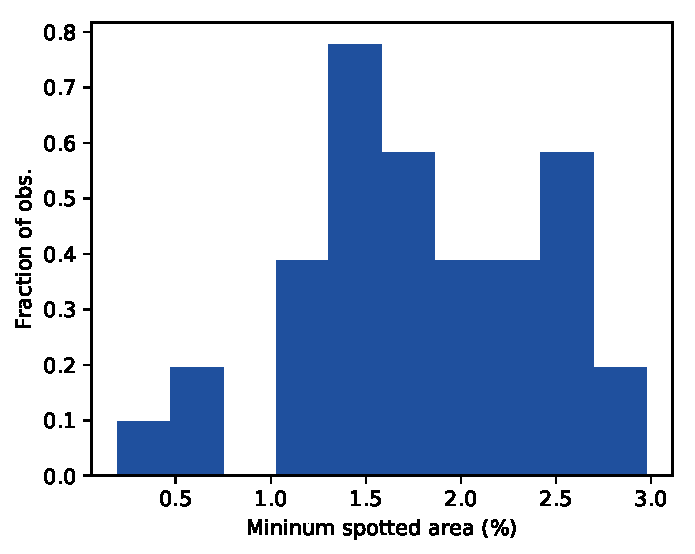
\includegraphics[scale=0.65]{stsp_hat_p_11/flux_deficit.pdf}
\caption{Minimum spot coverage of HAT-P-11, independently inferred from the flux deficits in the out-of-transit portions of the \kepler\ light curve. The minimum spot coverage in the range $0.5$ to $3\%$ is consistent with the spot coverage inferred from the spotted area in the transit chord in the maximum-likelihood \stsp\ models, $f_S = 3^{+6}_{-1} \% $.}
\label{fig:flux_deficit}
\end{figure}

The rotational modulation of the out-of-transit fluxes can independently constrain the spotted area of HAT-P-11 (for an assumed spot contrast). The difference between the brightest and dimmest flux measured in each \kepler\ quarter is equivalent to the product of the fractional projected spotted area and $1-c$, where $c$ is the spot contrast as defined in Equation~\ref{eqn:contrast}. 

In practice, the estimate of the spotted area via the flux deficit is a lower limit on the total spotted area. If there were only a few small spots on the star, the flux deficit would yield the true spot covering fraction. However in the limit of many small spots distributed evenly across the star, each spot that rotates out of view will be replaced by another spot rotating into view, and thus adding more spots would not increase the flux deficit. As we argue in this section and Section~\ref{sec:spot_number}, there are a significant number of spots on the star, and it is unclear if the star is in this saturated flux deficit regime. Thus the spotted area inferred by the flux deficit should be treated as a lower limit on the spotted area.

We compute the fractional spotted area for each \kepler\ quarter from the flux deficit as follows. We mask out all transits, and convolve the fluxes with a Gaussian kernel ($\sigma=50$ fluxes). We normalize each quarter's fluxes by its smoothed maximum flux. The minimum fractional spotted area during each quarter is given by $f_S = \left( 1 - \min\textrm{(flux)} \right)/(1-c)$.

The minimum spotted area inferred by the quarterly flux deficits is shown in Figure~\ref{fig:flux_deficit}. We see that minimum spotted area ranges from 0.1\% to 3\% over the different \kepler\ quarters. This is consistent with the 0.5-10\% spotted area that we infer from modeling spots in the transit chord (Figure~\ref{fig:spotted_area}).  


\subsection{Spot number} \label{sec:spot_number}

During the solar activity cycle, the number of spot groups observed on the Sun at any instant varies from near zero at activity minimum to hundreds at maximum. We measure the number of high-signal spot occultations per transit for HAT-P-11, which we can use to (1) search for evolution in the spot number over time; and (2) to compare to the number of sunspots.

The simplest measurement of the number of starspots that we can obtain from the \kepler\ photometry is the number of spots per transit for all 205 transits. Each transit is short compared to the expected spot evolution timescale (weeks) and the stellar rotation period ($29.2$ d), so each transit gives an instantaneous measurement of the number of spots within the transit chord. These spot numbers of HAT-P-11 are not directly comparable to sunspot numbers because solar observations can resolve much smaller spots than occultation photometry. It is also likely that what appear to be large spots in occultation photometry might really be groups of smaller spots at higher resolution.

We assume that the observed spot count per transit follows a Poisson distribution, and compute the likelihood of detecting the observed spot numbers for a given Poisson rate parameter $\lambda$ (with units of spots detected per transit). We allow the spot count rate to vary as a function of time, as it would throughout the solar activity cycle. We model the number of spots observed per transit with a Poisson distribution $P(\lambda)$ with a linearly varying Poisson rate parameter $\lambda(t) = \lambda_0 (t-t_0) + \lambda_1$, where $\lambda_0$ is the rate of change of the Poisson rate parameter over time (i.e.: how many more/less spots will be counted per year), and $\lambda_1$ is the rate parameter at time $t_0$. We marginalize over the hyperparameters with MCMC and find that the rate parameter slope is $\lambda_0 = 0.12 \pm 0.06$ spots per year. Since this slope is consistent with no slope, we fix $\lambda_0 = 0$ and solve only for a constant rate parameter, and find $\lambda = 0.870 \pm 0.066$ spots per transit.

The apparently constant spot number over four years could be observed for a Sun-like star with period $\sim11$ years if observed near maximum or minimum, or at any phase if the activity cycle has a long period. Spectroscopic activity index measurements over time may distinguish between these two possible cases. 

We can compute a rough estimate of the number of spots on the entire stellar surface by extrapolating from number of spots observed within each transit chord. The occulted fraction of the entire stellar surface area, $A_* = 4\pi R_*^2$, within each transit chord is $\sim 2.9\%$. If we assume there are $\lambda=0.87$ spots per transit from the analysis above, then there are $\sim 30 \pm 2$ spots like the ones detected in transit on the surface of the entire star at any given time, and about $15 \pm 1$ on the observer-facing hemisphere of the star.

We refrain from comparing the number of spots on HAT-P-11 to the common solar spot group number because solar observations are not directly analogous to the \kepler\ photometry. Ground-based observations of the Sun can observe sunspots as small as $R_{spot} = 1750$ km -- well below the smallest spots detected with high confidence on HAT-P-11 via transit photometry. However, we can compare the number of sunspots with radii as large as HAT-P-11's. The turnover in spot frequency for small spots on HAT-P-11 suggests that we are insensitive to spots with $R_{spot,min} < 2 \times 10^4$ km (see Figure~\ref{fig:radii}). We identify 898 spots larger than $2 \times 10^4$ km  observed over 10818 days on the Sun \citep{Howard1984}, which is roughly a rate of $0.08$ spots on the observer-facing hemisphere of the Sun at any instant. On HAT-P-11 we detect 130 such spots in 205 transits. The transit chord of HAT-P-11 b spans 6\% of the observer-facing hemisphere, so we expect roughly 11 spots on HAT-P-11 at any instant with radii $>2 \times 10^4$ km. Clearly there are more spots on HAT-P-11 of this size than on the Sun.

In light of the large spot number of HAT-P-11, and the sunspot-like radii of its spots, we can now interpret the spot area determined in Section~\ref{sec:spotted_area}. The spotted area on HAT-P-11 is 100x greater than solar largely due to the presence of \textit{more} spots, since the spot radii are typically quite similar to large sunspots near solar maximum (see spot radius discussion in Section~\ref{sec:radii}). 

\section{Conclusions and discussion} \label{sec:conclusion}

We have measured the properties of starspots on the active K4 dwarf HAT-P-11 from \kepler\ photometry of its transiting planet. We take advantage of the planet's well known orbital orientation to measure starspot positions during occultations by the planet. The highly misaligned orbit of the planet allows us to unambiguously resolve spot latitudes.

The spots of HAT-P-11 are similar to the Sun's in several ways. The spot contrast is consistent with the area-weighted contrast of typical sunspots, $c=0.3$ (Eqn.~\ref{eqn:contrast}). The mode of the spot radius distribution is similar to the radii of sunspots at solar maximum. The active latitudes of HAT-P-11 have the same mean latitude and standard deviation as the Sun at solar maximum. The asymmetry in the number of spots in each hemisphere is consistent with the range of values observed on the Sun. 

However, the activity of HAT-P-11 is more extreme than the Sun's. The mean spot coverage from 2009-2013 is $3^{+6}_{-1}\%$, $\sim$100x greater than the Sun's. The number of large starspots is roughly 100x greater than the number of similarly sized spots on the Sun. The $S$-index of HAT-P-11 is a factor of two greater than one would expect by extrapolating from the spot coverage--$S$-index relation observed on the Sun.

The similarities between the spot distributions on the Sun and HAT-P-11 are interesting in the context of dynamo theory \citep[e.g.][]{Charbonneau2010}. This K4 star is not fully convective, and therefore is expected to have a tachocline like the Sun. Perhaps the $\alpha\Omega$ dynamo is operating within HAT-P-11 as it does in the Sun. It seems that a $0.8M_\odot$ star with a near-solar rotation rate produces starspots in strikingly similar active latitudes, with more large spots. The theoretical prescriptions for magnetic flux emergence developed for the Sun may therefore be applicable out to spectral type K4 \citep[e.g.][]{Cheung2014}.

Precision spot occultation analysis made possible by \kepler\ could potentially be reproduced with photometry from NASA's TESS mission for HAT-P-11 in particular, and for active planet-host stars in general \citep{Ricker2014}. However, the one-minute cadence photometry was critical for resolving the spot occultation features of HAT-P-11, and time resolution directly translates to latitude resolution for highly misaligned systems. The TESS mission's planned two-minute cadence is likely sufficient to detect spot occultations in systems like HAT-P-11, though shorter cadence ground-based photometry would be preferred.

\subsection{Future Work}

HAT-P-11 is exceptionally bright ($V=9.47$), which makes ground-based observations of spot occultations with amplitudes on the order of 0.1\% feasible. In particular, we plan to collect transit photometry with the holographic diffuser and the ARCTIC imager on the ARC 3.5 m Telescope at the Apache Point Observatory (APO) (Stef\'{a}nsson et al.~2017, submitted). If HAT-P-11 exhibits evolution in the spot latitude distribution like the Sun does, we may be able to observe changes in the mean spot position as the activity cycle progresses. Observing spot occultations from the ground is advantageous because the latitude resolution is linked to the time resolution of the photometry, which can be minimized with large aperture telescopes and thus shorter exposure times compared to \kepler\ or TESS.

The phase of the activity cycle of HAT-P-11 can be constrained over several years by analyzing long-term spectroscopy of the $S$-index. In Morris et al.~(2017, in prep), we constrain the period and amplitude of the activity cycle of HAT-P-11 using archival high resolution spectroscopy of the star, in combination with recent high resolution spectra obtained at APO.

The constraints on the spot coverage of HAT-P-11 from the \kepler\ photometry are complementary to spectroscopic constraints from molecular band modeling. The spot coverage reported here could be independently measured by modeling absorption by TiO and OH in starspots \citep{ONeal2001, ONeal2004}. 

In this work we limited ourselves to studying only the spot occultations in transit to make direct comparisons between spots on HAT-P-11 and sunspots. Simultaneous modeling of the out-of-transit fluxes would provide complementary constraints on the total spot coverage on HAT-P-11. 

% \acknowledgments

% We acknowledge support from NSF grant AST-1312453. We thank Eric Agol, John Lurie, Dan Foreman-Mackey and Charli Sakari for constructive conversations during the development of this work.

% Some of the data presented in this paper were obtained from the Mikulski Archive for Space Telescopes (MAST). STScI is operated by the Association of Universities for Research in Astronomy, Inc., under NASA contract NAS5-26555. Support for MAST for non-HST data is provided by the NASA Office of Space Science via grant NNX09AF08G and by other grants and contracts. This research has made use of NASA's Astrophysics Data System. This work used the Extreme Science and Engineering Discovery Environment (XSEDE), which is supported by National Science Foundation grant number ACI-1548562. This research was done using resources provided by the Open Science Grid [1,2], which is supported by the National Science Foundation award 1148698, and the U.S. Department of Energy's Office of Science. This work was facilitated though the use of advanced computational, storage, and networking infrastructure provided by the Hyak supercomputer system and funded by the STF at the University of Washington.

% \facility{Kepler}

% \software{STSP \citep{Hebb2017}, \texttt{ipython} \citep{ipython}, \texttt{numpy} \citep{VanDerWalt2011}, \texttt{scipy} \citep{scipy},  \texttt{matplotlib} \citep{matplotlib}, \texttt{astropy} \citep{Astropy2013}, \texttt{batman} \citep{Kreidberg2015}, \texttt{gatspy} \citep{gatspy}}

% \appendix

\begin{subappendices}
\section*{Spot contrast} \label{sec:appendix_contrast}

We make some simplifying assumptions to derive constraints on the spot contrast from the amplitudes of spot occultations, and we generalize the formalism later. We will at first calculate the flux only for spot-planet orientations where the planet completely occults the spot or the spot completely encompasses the planet. By ignoring grazing spot occultations, we will calculate maximum spot-occultation amplitudes, since grazing spot occultations yield smaller amplitudes than complete occultations. We also ignore stellar limb darkening.

The flux lost during the transit of a planet with radius $R_p$ across an unspotted star with radius $R_\star$ without limb darkening is
\begin{eqnarray}
\delta_{unspotted} = \frac{\Delta F}{F_\star} = \frac{I_\star \pi R_p^2}{I_\star \pi R_\star^2} = \frac{R_p^2}{R_\star^2}
\end{eqnarray}
where $I_\star$ is the mean surface intensity of the stellar disk per unit area. 
\begin{figure}
\centering
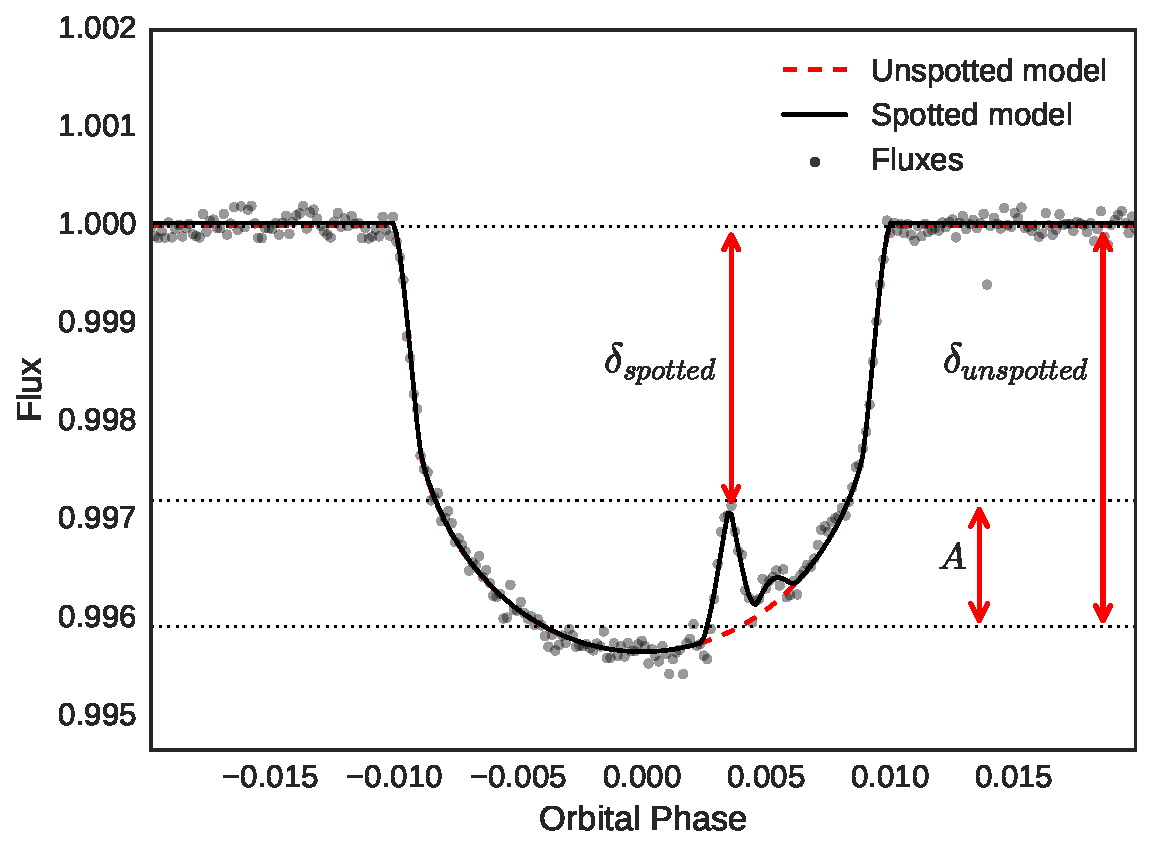
\includegraphics[scale=0.4]{stsp_hat_p_11/contrast_schematic.pdf}
\caption{Schematic for parameter definitions in Section~\ref{sec:contrast}, plotted on the transit of HAT-P-11 b on August 20, 2011 UT. The spot occultation amplitude $A$ is the difference between the flux lost during a transit with no spot occultations and the flux lost during a transit with spot occultations, $A = \delta_{unspotted} - \delta_{spotted}$. Note that in this terminology the ``depth'' $\delta(\mu) = \Delta F(\mu)/F$ is a function of the sky-projected distance between the planet and the star $\mu$, or equivalently time or orbital phase, for a star with limb-darkening.}
\label{fig:contrast_schematic}
\end{figure}

We measure the amplitude of brightening during a spot occultation $A$, see Figure~\ref{fig:contrast_schematic} for a schematic representation. During an occultation of a starspot, the appropriate formula for the observed flux depends on the size of the spot $R_{sp}$ relative to the size of the planet $R_{p}$. If the spot with radius larger than or equal to the radius of the planet $R_{sp} \ge R_p$ and the spot has contrast $c$, the amplitude of the difference in flux between a transit of an unspotted and a spotted star is
\begin{eqnarray}
 A &=& \left. \delta_{unspotted} - \delta_{spotted} \right|_{R_{sp} > R_p} \\
 &=& \frac{I_\star \pi R_p^2}{I_\star \pi R_\star^2} - \frac{((1 - c)I_\star) \pi R_p^2}{ I_\star \pi R_\star^2}\\
A/\delta_{unspotted} &=&  c. \label{eqn:bigspot}
\end{eqnarray}
For a spot smaller than the planet, the difference between the spotted and unspotted flux is
\begin{eqnarray}
 A &=& \left. \delta_{unspotted} - \delta_{spotted} \right|_{R_{sp} < R_p} \\
 &=& \frac{I_\star \pi R_p^2}{I_\star \pi R_\star^2} - \frac{I_\star \pi R_p^2 - c I_\star \pi R_p^2 R_{sp}^2/R_p^2}{ I_\star \pi R_\star^2}\\
 A/\delta_{unspotted} &=&  c \left(\frac{R_{sp}}{R_p}\right)^2
 \label{eqn:littlespot}
\end{eqnarray}

In the small planet limit where $R_p/R_\star \ll 1$, the stellar limb darkening could be defined, for example, with a quadratic law $I(\mu)/I_0 = 1 - u_1(1-\mu) - u_2(1-\mu)^2$, and the instantaneous unspotted depth becomes 
\begin{equation}
\delta_{unspotted}(\mu) =  \frac{R_p^2}{R_\star^2} \left[ \frac{1 - u_1(1-\mu) - u_2(1-\mu)^2}{1 - \frac{1}{3}u_1 - \frac{1}{6}u_2} \right]
\end{equation}
where $\mu$ is the sky-projected distance between the planet and the star. Equations \ref{eqn:bigspot} and \ref{eqn:littlespot} above can be generalized for stars with limb-darkening by replacing $\delta_{unspotted} \rightarrow \delta_{unspotted}(\mu)$.

\end{subappendices}

%\bibliographystyle{apj}
%\bibliography{stsp_hat_p_11/bibliography}

% \bibliography{stsp_hat_p_11/bibliography.bib}
% \begin{thebibliography}{}

% \bibitem[\protect\astroncite{{Astropy Collaboration}
%   et~al.}{2013}]{Astropy2013}
% {Astropy Collaboration}, T.~P. {Robitaille}, E.~J. {Tollerud}, P.~{Greenfield},
%   M.~{Droettboom}, E.~{Bray}, T.~{Aldcroft}, M.~{Davis}, A.~{Ginsburg}, A.~M.
%   {Price-Whelan}, W.~E. {Kerzendorf}, A.~{Conley}, N.~{Crighton}, K.~{Barbary},
%   D.~{Muna}, H.~{Ferguson}, F.~{Grollier}, M.~M. {Parikh}, P.~H. {Nair}, H.~M.
%   {Unther}, C.~{Deil}, J.~{Woillez}, S.~{Conseil}, R.~{Kramer}, J.~E.~H.
%   {Turner}, L.~{Singer}, R.~{Fox}, B.~A. {Weaver}, V.~{Zabalza}, Z.~I.
%   {Edwards}, K.~{Azalee Bostroem}, D.~J. {Burke}, A.~R. {Casey}, S.~M.
%   {Crawford}, N.~{Dencheva}, J.~{Ely}, T.~{Jenness}, K.~{Labrie}, P.~{Lian
%   Lim}, F.~{Pierfederici}, A.~{Pontzen}, A.~{Ptak}, B.~{Refsdal},
%   M.~{Servillat}, and O.~{Streicher}\leavevmode\nopagebreak\newline 2013.
% \newblock {Astropy: A community Python package for astronomy}.
% \newblock {\em \aap}, 558:A33.

% \bibitem[\protect\astroncite{{Babcock}}{1961}]{Babcock1961}
% {Babcock}, H.~W.\leavevmode\nopagebreak\newline 1961.
% \newblock {The Topology of the Sun's Magnetic Field and the 22-YEAR Cycle.}
% \newblock {\em \apj}, 133:572.

% \bibitem[\protect\astroncite{{Bakos} et~al.}{2010}]{Bakos2010}
% {Bakos}, G.~{\'A}., G.~{Torres}, A.~{P{\'a}l}, J.~{Hartman}, G.~{Kov{\'a}cs},
%   R.~W. {Noyes}, D.~W. {Latham}, D.~D. {Sasselov}, B.~{Sip{\H o}cz}, G.~A.
%   {Esquerdo}, D.~A. {Fischer}, J.~A. {Johnson}, G.~W. {Marcy}, R.~P. {Butler},
%   H.~{Isaacson}, A.~{Howard}, S.~{Vogt}, G.~{Kov{\'a}cs}, J.~{Fernandez},
%   A.~{Mo{\'o}r}, R.~P. {Stefanik}, J.~{L{\'a}z{\'a}r}, I.~{Papp}, and
%   P.~{S{\'a}ri}\leavevmode\nopagebreak\newline 2010.
% \newblock {HAT-P-11b: A Super-Neptune Planet Transiting a Bright K Star in the
%   Kepler Field}.
% \newblock {\em \apj}, 710:1724--1745.

% \bibitem[\protect\astroncite{{Balmaceda} et~al.}{2009}]{Balmaceda2009}
% {Balmaceda}, L.~A., S.~K. {Solanki}, N.~A. {Krivova}, and
%   S.~{Foster}\leavevmode\newline 2009.
% \newblock {A homogeneous database of sunspot areas covering more than 130
%   years}.
% \newblock {\em Journal of Geophysical Research (Space Physics)}, 114:A07104.

% \bibitem[\protect\astroncite{{B{\'e}ky} et~al.}{2014a}]{Beky2014a}
% {B{\'e}ky}, B., M.~J. {Holman}, D.~M. {Kipping}, and R.~W.
%   {Noyes}\leavevmode\nopagebreak\newline 2014a.
% \newblock {Stellar Rotation-Planetary Orbit Period Commensurability in the
%   HAT-P-11 System}.
% \newblock {\em \apj}, 788:1.

% \bibitem[\protect\astroncite{{B{\'e}ky} et~al.}{2014b}]{Beky2014b}
% {B{\'e}ky}, B., D.~M. {Kipping}, and M.~J.
%   {Holman}\leavevmode\nopagebreak\newline 2014b.
% \newblock {SPOTROD: a semi-analytic model for transits of spotted stars}.
% \newblock {\em \mnras}, 442:3686--3699.

% \bibitem[\protect\astroncite{{Berdyugina}}{2005}]{Berdyugina2005}
% {Berdyugina}, S.~V.\leavevmode\nopagebreak\newline 2005.
% \newblock {Starspots: A Key to the Stellar Dynamo}.
% \newblock {\em Living Reviews in Solar Physics}, 2:8.

% \bibitem[\protect\astroncite{{Carbonell} et~al.}{1993}]{Carbonell1993}
% {Carbonell}, M., R.~{Oliver}, and J.~L.
%   {Ballester}\leavevmode\nopagebreak\newline 1993.
% \newblock {On the asymmetry of solar activity}.
% \newblock {\em \aap}, 274:497.

% \bibitem[\protect\astroncite{{Carter} et~al.}{2011}]{Carter2011}
% {Carter}, J.~A., J.~N. {Winn}, M.~J. {Holman}, D.~{Fabrycky}, Z.~K. {Berta},
%   C.~J. {Burke}, and P.~{Nutzman}\leavevmode\nopagebreak\newline 2011.
% \newblock {The Transit Light Curve Project. XIII. Sixteen Transits of the
%   Super-Earth GJ 1214b}.
% \newblock {\em \apj}, 730:82.

% \bibitem[\protect\astroncite{Charbonneau}{2010}]{Charbonneau2010}
% Charbonneau, P.\leavevmode\nopagebreak\newline 2010.
% \newblock Dynamo models of the solar cycle.
% \newblock {\em Living Reviews in Solar Physics}, 7(1):3.

% \bibitem[\protect\astroncite{Cheung and Isobe}{2014}]{Cheung2014}
% Cheung, M. C.~M. and H.~Isobe\leavevmode\nopagebreak\newline 2014.
% \newblock Flux emergence (theory).
% \newblock {\em Living Reviews in Solar Physics}, 11(1):3.

% \bibitem[\protect\astroncite{{Christensen-Dalsgaard}
%   et~al.}{2010}]{Christensen-Dalsgaard2010}
% {Christensen-Dalsgaard}, J., H.~{Kjeldsen}, T.~M. {Brown}, R.~L. {Gilliland},
%   T.~{Arentoft}, S.~{Frandsen}, P.-O. {Quirion}, W.~J. {Borucki}, D.~{Koch},
%   and J.~M. {Jenkins}\leavevmode\nopagebreak\newline 2010.
% \newblock {Asteroseismic Investigation of Known Planet Hosts in the Kepler
%   Field}.
% \newblock {\em \apjl}, 713:L164--L168.

% \bibitem[\protect\astroncite{{Cincunegui} et~al.}{2007}]{Cincunegui2007}
% {Cincunegui}, C., R.~F. {D{\'{\i}}az}, and P.~J.~D.
%   {Mauas}\leavevmode\nopagebreak\newline 2007.
% \newblock {H{$\alpha$} and the Ca II H and K lines as activity proxies for
%   late-type stars}.
% \newblock {\em \aap}, 469:309--317.

% \bibitem[\protect\astroncite{{Csizmadia} et~al.}{2013}]{Csizmadia2013}
% {Csizmadia}, S., T.~{Pasternacki}, C.~{Dreyer}, J.~{Cabrera}, A.~{Erikson}, and
%   H.~{Rauer}\leavevmode\nopagebreak\newline 2013.
% \newblock {The effect of stellar limb darkening values on the accuracy of the
%   planet radii derived from photometric transit observations}.
% \newblock {\em \aap}, 549:A9.

% \bibitem[\protect\astroncite{{Czesla} et~al.}{2009}]{Czesla2009}
% {Czesla}, S., K.~F. {Huber}, U.~{Wolter}, S.~{Schr{\"o}ter}, and J.~H.~M.~M.
%   {Schmitt}\leavevmode\nopagebreak\newline 2009.
% \newblock {How stellar activity affects the size estimates of extrasolar
%   planets}.
% \newblock {\em \aap}, 505:1277--1282.

% \bibitem[\protect\astroncite{{Deming} et~al.}{2011}]{Deming2011}
% {Deming}, D., P.~V. {Sada}, B.~{Jackson}, S.~W. {Peterson}, E.~{Agol}, H.~A.
%   {Knutson}, D.~E. {Jennings}, F.~{Haase}, and
%   K.~{Bays}\leavevmode\nopagebreak\newline 2011.
% \newblock {Kepler and Ground-based Transits of the Exo-Neptune HAT-P-11b}.
% \newblock {\em \apj}, 740:33.

% \bibitem[\protect\astroncite{{Egeland} et~al.}{2017}]{Egeland2017}
% {Egeland}, R., W.~{Soon}, S.~{Baliunas}, J.~C. {Hall}, A.~A. {Pevtsov}, and
%   L.~{Bertello}\leavevmode\nopagebreak\newline 2017.
% \newblock {The Mount Wilson Observatory S-index of the Sun}.
% \newblock {\em \apj}, 835:25.

% \bibitem[\protect\astroncite{{Fabrycky} and {Winn}}{2009}]{Fabrycky2009}
% {Fabrycky}, D.~C. and J.~N. {Winn}\leavevmode\nopagebreak\newline 2009.
% \newblock {Exoplanetary Spin-Orbit Alignment: Results from the Ensemble of
%   Rossiter-McLaughlin Observations}.
% \newblock {\em \apj}, 696:1230--1240.

% \bibitem[\protect\astroncite{{Foreman-Mackey}
%   et~al.}{2013}]{Foreman-Mackey2013}
% {Foreman-Mackey}, D., D.~W. {Hogg}, D.~{Lang}, and
%   J.~{Goodman}\leavevmode\nopagebreak\newline 2013.
% \newblock {emcee: The MCMC Hammer}.
% \newblock {\em \pasp}, 125:306--312.

% \bibitem[\protect\astroncite{{Goodman} and {Weare}}{2010}]{Goodman2010}
% {Goodman}, J. and J.~{Weare}\leavevmode\nopagebreak\newline 2010.
% \newblock {Ensemble samplers with affine invariance}.
% \newblock {\em Communications in Applied Mathematics and Computational
%   Science}, 5:65--80.

% \bibitem[\protect\astroncite{{Hathaway}}{2011}]{Hathaway2011}
% {Hathaway}, D.~H.\leavevmode\nopagebreak\newline 2011.
% \newblock {A Standard Law for the Equatorward Drift of the Sunspot Zones}.
% \newblock {\em \solphys}, 273:221--230.

% \bibitem[\protect\astroncite{{Hathaway}}{2015}]{Hathaway2015}
% {Hathaway}, D.~H.\leavevmode\nopagebreak\newline 2015.
% \newblock {The Solar Cycle}.
% \newblock {\em Living Reviews in Solar Physics}, 12.

% \bibitem[\protect\astroncite{{Hebb} et~al.}{2017}]{Hebb2017}
% {Hebb}, L., {Rohn}, G., et al.\leavevmode\nopagebreak\newline 2017 (in prep.).
% \newblock {STSP: A starspot occultation model}.

% \bibitem[\protect\astroncite{{Hirano} et~al.}{2011}]{Hirano2011}
% {Hirano}, T., N.~{Narita}, A.~{Shporer}, B.~{Sato}, W.~{Aoki}, and
%   M.~{Tamura}\leavevmode\nopagebreak\newline 2011.
% \newblock {A Possible Tilted Orbit of the Super-Neptune HAT-P-11b}.
% \newblock {\em \pasj}, 63:531--.

% \bibitem[\protect\astroncite{{Howard} et~al.}{1984}]{Howard1984}
% {Howard}, R., P.~I. {Gilman}, and P.~A. {Gilman}\leavevmode\nopagebreak\newline
%   1984.
% \newblock {Rotation of the sun measured from Mount Wilson white-light images}.
% \newblock {\em \apj}, 283:373--384.

% \bibitem[\protect\astroncite{{Hunter}}{2007}]{matplotlib}
% {Hunter}, J.~D.\leavevmode\nopagebreak\newline 2007.
% \newblock {Matplotlib: A 2D Graphics Environment}.
% \newblock {\em Computing in Science and Engineering}, 9:90--95.

% \bibitem[\protect\astroncite{{Husser} et~al.}{2013}]{Husser2013}
% {Husser}, T.-O., S.~{Wende-von Berg}, S.~{Dreizler}, D.~{Homeier},
%   A.~{Reiners}, T.~{Barman}, and P.~H.
%   {Hauschildt}\leavevmode\nopagebreak\newline 2013.
% \newblock {A new extensive library of PHOENIX stellar atmospheres and synthetic
%   spectra}.
% \newblock {\em \aap}, 553:A6.

% \bibitem[\protect\astroncite{Jones et~al.}{01  }]{scipy}
% Jones, E., T.~Oliphant, P.~Peterson, et~al.\leavevmode\nopagebreak\newline
%   2001--.
% \newblock {SciPy}: Open source scientific tools for {Python}.
% \newblock [Online; accessed <today>].

% \bibitem[\protect\astroncite{{Keppens} and {Martinez
%   Pillet}}{1996}]{Keppens1996}
% {Keppens}, R. and V.~{Martinez Pillet}\leavevmode\nopagebreak\newline 1996.
% \newblock {The magnetic structure of pores and sunspots derived from Advanced
%   Stokes Polarimeter data.}
% \newblock {\em \aap}, 316:229--242.

% \bibitem[\protect\astroncite{{Kipping}}{2013}]{Kipping2013}
% {Kipping}, D.~M.\leavevmode\nopagebreak\newline 2013.
% \newblock {Efficient, uninformative sampling of limb darkening coefficients for
%   two-parameter laws}.
% \newblock {\em \mnras}, 435:2152--2160.

% \bibitem[\protect\astroncite{{Kreidberg}}{2015}]{Kreidberg2015}
% {Kreidberg}, L.\leavevmode\nopagebreak\newline 2015.
% \newblock {BATMAN: BAsic Transit Model cAlculatioN in Python}.
% \newblock {\em \pasp}, 127:1161--1165.

% \bibitem[\protect\astroncite{{Leonard} and {Choudhary}}{2008}]{Leonard2008}
% {Leonard}, T. and D.~P. {Choudhary}\leavevmode\nopagebreak\newline 2008.
% \newblock {Intensity and Magnetic Field Distribution of Sunspots}.
% \newblock {\em \solphys}, 252:33--41.

% \bibitem[\protect\astroncite{{Li} et~al.}{2002}]{Li2002}
% {Li}, K.-J., X.-H. {Liu}, H.-S. {Yun}, S.-Y. {Xiong}, H.-F. {Liang}, H.-Z.
%   {Zhao}, L.-S. {Zhan}, and X.-M. {Gu}\leavevmode\nopagebreak\newline 2002.
% \newblock {Asymmetrical Distribution of Sunspot Groups in the Solar
%   Hemispheres}.
% \newblock {\em \pasj}, 54:629--633.

% \bibitem[\protect\astroncite{{Mandel} and {Agol}}{2002}]{Mandel2002}
% {Mandel}, K. and E.~{Agol}\leavevmode\nopagebreak\newline 2002.
% \newblock {Analytic Light Curves for Planetary Transit Searches}.
% \newblock {\em \apjl}, 580:L171--L175.

% \bibitem[\protect\astroncite{{Neff} et~al.}{1995}]{Neff1995}
% {Neff}, J.~E., D.~{O'Neal}, and S.~H. {Saar}\leavevmode\nopagebreak\newline
%   1995.
% \newblock {Absolute Measurements of Starspot Area and Temperature: II Pegasi in
%   1989 October}.
% \newblock {\em \apj}, 452:879.

% \bibitem[\protect\astroncite{{Newton}}{1955}]{Newton1955}
% {Newton}, H.~W.\leavevmode\nopagebreak\newline 1955.
% \newblock {The lineage of the great sunspots}.
% \newblock {\em Vistas in Astronomy}, 1:666--674.

% \bibitem[\protect\astroncite{{Ohta} et~al.}{2005}]{Ohta2005}
% {Ohta}, Y., A.~{Taruya}, and Y.~{Suto}\leavevmode\nopagebreak\newline 2005.
% \newblock {The Rossiter-McLaughlin Effect and Analytic Radial Velocity Curves
%   for Transiting Extrasolar Planetary Systems}.
% \newblock {\em \apj}, 622:1118--1135.

% \bibitem[\protect\astroncite{{O'Neal} et~al.}{2004}]{ONeal2004}
% {O'Neal}, D., J.~E. {Neff}, S.~H. {Saar}, and
%   M.~{Cuntz}\leavevmode\nopagebreak\newline 2004.
% \newblock {Further Results of TiO-Band Observations of Starspots}.
% \newblock {\em \aj}, 128:1802--1811.

% \bibitem[\protect\astroncite{{O'Neal} et~al.}{2001}]{ONeal2001}
% {O'Neal}, D., J.~E. {Neff}, S.~H. {Saar}, and J.~K.
%   {Mines}\leavevmode\nopagebreak\newline 2001.
% \newblock {Hydroxyl 1.563 Micron Absorption from Starspots on Active Stars}.
% \newblock {\em \aj}, 122:1954--1964.

% \bibitem[\protect\astroncite{{O'Neal} et~al.}{1996}]{ONeal1996}
% {O'Neal}, D., S.~H. {Saar}, and J.~E. {Neff}\leavevmode\nopagebreak\newline
%   1996.
% \newblock {Measurements of Starspot Area and Temperature on Five Active,
%   Evolved Stars}.
% \newblock {\em \apj}, 463:766.

% \bibitem[\protect\astroncite{{Pace}}{2013}]{Pace2013}
% {Pace}, G.\leavevmode\nopagebreak\newline 2013.
% \newblock {Chromospheric activity as age indicator. An L-shaped
%   chromospheric-activity versus age diagram}.
% \newblock {\em \aap}, 551:L8.

% \bibitem[\protect\astroncite{{Parker}}{1955a}]{Parker1955b}
% {Parker}, E.~N.\leavevmode\nopagebreak\newline 1955a.
% \newblock {Hydromagnetic Dynamo Models.}
% \newblock {\em \apj}, 122:293.

% \bibitem[\protect\astroncite{{Parker}}{1955b}]{Parker1955a}
% {Parker}, E.~N.\leavevmode\nopagebreak\newline 1955b.
% \newblock {The Formation of Sunspots from the Solar Toroidal Field.}
% \newblock {\em \apj}, 121:491.

% \bibitem[\protect\astroncite{Perez and Granger}{2007}]{ipython}
% Perez, F. and B.~E. Granger\leavevmode\nopagebreak\newline 2007.
% \newblock Ipython: A system for interactive scientific computing.
% \newblock {\em Computing in Science and Engg.}, 9(3):21--29.

% \bibitem[\protect\astroncite{{Petit} et~al.}{2008}]{Petit2008}
% {Petit}, P., B.~{Dintrans}, S.~K. {Solanki}, J.-F. {Donati}, M.~{Auri{\`e}re},
%   F.~{Ligni{\`e}res}, J.~{Morin}, F.~{Paletou}, J.~{Ramirez Velez},
%   C.~{Catala}, and R.~{Fares}\leavevmode\nopagebreak\newline 2008.
% \newblock {Toroidal versus poloidal magnetic fields in Sun-like stars: a
%   rotation threshold}.
% \newblock {\em \mnras}, 388:80--88.

% \bibitem[\protect\astroncite{Pordes et~al.}{2007}]{osg}
% Pordes, R., D.~Petravick, B.~Kramer, D.~Olson, M.~Livny, A.~Roy, P.~Avery,
%   K.~Blackburn, T.~Wenaus, F.~Würthwein, I.~Foster, R.~Gardner, M.~Wilde,
%   A.~Blatecky, J.~McGee, and R.~Quick\leavevmode\nopagebreak\newline 2007.
% \newblock The open science grid.
% \newblock {\em Journal of Physics: Conference Series}, 78(1):012057.

% \bibitem[\protect\astroncite{{Reiners}}{2012}]{Reiners2012}
% {Reiners}, A.\leavevmode\nopagebreak\newline 2012.
% \newblock {Observations of Cool-Star Magnetic Fields}.
% \newblock {\em Living Reviews in Solar Physics}, 9:1.

% \bibitem[\protect\astroncite{{Ricker} et~al.}{2014}]{Ricker2014}
% {Ricker}, G.~R., J.~N. {Winn}, R.~{Vanderspek}, D.~W. {Latham}, G.~{\'A}.
%   {Bakos}, J.~L. {Bean}, Z.~K. {Berta-Thompson}, T.~M. {Brown}, L.~{Buchhave},
%   N.~R. {Butler}, R.~P. {Butler}, W.~J. {Chaplin}, D.~{Charbonneau},
%   J.~{Christensen-Dalsgaard}, M.~{Clampin}, D.~{Deming}, J.~{Doty}, N.~{De
%   Lee}, C.~{Dressing}, E.~W. {Dunham}, M.~{Endl}, F.~{Fressin}, J.~{Ge},
%   T.~{Henning}, M.~J. {Holman}, A.~W. {Howard}, S.~{Ida}, J.~{Jenkins},
%   G.~{Jernigan}, J.~A. {Johnson}, L.~{Kaltenegger}, N.~{Kawai}, H.~{Kjeldsen},
%   G.~{Laughlin}, A.~M. {Levine}, D.~{Lin}, J.~J. {Lissauer}, P.~{MacQueen},
%   G.~{Marcy}, P.~R. {McCullough}, T.~D. {Morton}, N.~{Narita}, M.~{Paegert},
%   E.~{Palle}, F.~{Pepe}, J.~{Pepper}, A.~{Quirrenbach}, S.~A. {Rinehart},
%   D.~{Sasselov}, B.~{Sato}, S.~{Seager}, A.~{Sozzetti}, K.~G. {Stassun},
%   P.~{Sullivan}, A.~{Szentgyorgyi}, G.~{Torres}, S.~{Udry}, and
%   J.~{Villasenor}\leavevmode\nopagebreak\newline 2014.
% \newblock {Transiting Exoplanet Survey Satellite (TESS)}.
% \newblock In {\em Space Telescopes and Instrumentation 2014: Optical, Infrared,
%   and Millimeter Wave}, volume 9143 of {\em \procspie}, P.~ 914320.

% \bibitem[\protect\astroncite{{Saar}}{1990}]{Saar1990}
% {Saar}, S.~H.\leavevmode\nopagebreak\newline 1990.
% \newblock {Magnetic Fields on Solar-like Stars: The First Decade}.
% \newblock In {\em Solar Photosphere: Structure, Convection, and Magnetic
%   Fields}, J.~O. {Stenflo}, ed., volume 138 of {\em IAU Symposium}, Pp.~
%   427--441.

% \bibitem[\protect\astroncite{{Sanchis-Ojeda} and
%   {Winn}}{2011}]{Sanchis-Ojeda2011}
% {Sanchis-Ojeda}, R. and J.~N. {Winn}\leavevmode\nopagebreak\newline 2011.
% \newblock {Starspots, Spin-Orbit Misalignment, and Active Latitudes in the
%   HAT-P-11 Exoplanetary System}.
% \newblock {\em \apj}, 743:61.

% \bibitem[\protect\astroncite{{Schrijver} and {Title}}{2001}]{Schrijver2001}
% {Schrijver}, C.~J. and A.~M. {Title}\leavevmode\nopagebreak\newline 2001.
% \newblock {On the Formation of Polar Spots in Sun-like Stars}.
% \newblock {\em \apj}, 551:1099--1106.

% \bibitem[\protect\astroncite{{Shapiro} et~al.}{2014}]{Shapiro2014}
% {Shapiro}, A.~I., S.~K. {Solanki}, N.~A. {Krivova}, W.~K. {Schmutz}, W.~T.
%   {Ball}, R.~{Knaack}, E.~V. {Rozanov}, and Y.~C.
%   {Unruh}\leavevmode\nopagebreak\newline 2014.
% \newblock {Variability of Sun-like stars: reproducing observed photometric
%   trends}.
% \newblock {\em \aap}, 569:A38.

% \bibitem[\protect\astroncite{{Solanki}}{2003}]{Solanki2003}
% {Solanki}, S.~K.\leavevmode\nopagebreak\newline 2003.
% \newblock {Sunspots: An overview}.
% \newblock {\em \aapr}, 11:153--286.

% \bibitem[\protect\astroncite{{Solanki} et~al.}{2013}]{Solanki2013}
% {Solanki}, S.~K., N.~A. {Krivova}, and J.~D.
%   {Haigh}\leavevmode\nopagebreak\newline 2013.
% \newblock {Solar Irradiance Variability and Climate}.
% \newblock {\em \araa}, 51:311--351.

% \bibitem[\protect\astroncite{{Solanki} and {Unruh}}{2004}]{Solanki2004}
% {Solanki}, S.~K. and Y.~C. {Unruh}\leavevmode\nopagebreak\newline 2004.
% \newblock {Spot sizes on Sun-like stars}.
% \newblock {\em \mnras}, 348:307--315.

% \bibitem[\protect\astroncite{{Southworth}}{2011}]{Southworth2011}
% {Southworth}, J.\leavevmode\nopagebreak\newline 2011.
% \newblock {Homogeneous studies of transiting extrasolar planets - IV. Thirty
%   systems with space-based light curves}.
% \newblock {\em \mnras}, 417:2166--2196.

% \bibitem[\protect\astroncite{Towns et~al.}{2014}]{xsede}
% Towns, J., T.~Cockerill, M.~Dahan, I.~Foster, K.~Gaither, A.~Grimshaw,
%   V.~Hazlewood, S.~Lathrop, D.~Lifka, G.~D. Peterson, R.~Roskies, J.~R. Scott,
%   and N.~Wilkins-Diehr\leavevmode\nopagebreak\newline 2014.
% \newblock Xsede: Accelerating scientific discovery.
% \newblock {\em Computing in Science \& Engineering}, 16(5):62--74.

% \bibitem[\protect\astroncite{{Van Der Walt} et~al.}{2011}]{VanDerWalt2011}
% {Van Der Walt}, S., S.~C. {Colbert}, and
%   G.~{Varoquaux}\leavevmode\nopagebreak\newline 2011.
% \newblock {The NumPy array: a structure for efficient numerical computation}.
% \newblock {\em ArXiv e-prints}.

% \bibitem[\protect\astroncite{Vanderplas}{2015}]{gatspy}
% Vanderplas, J.\leavevmode\nopagebreak\newline 2015.
% \newblock {gatspy: General tools for Astronomical Time Series in Python}.

% \bibitem[\protect\astroncite{{Vizoso} and {Ballester}}{1990}]{Vizoso1990}
% {Vizoso}, G. and J.~L. {Ballester}\leavevmode\nopagebreak\newline 1990.
% \newblock {The north-south asymmetry of sunspots}.
% \newblock {\em \aap}, 229:540--546.

% \bibitem[\protect\astroncite{{Waldmeier}}{1971}]{Waldmeier1971}
% {Waldmeier}, M.\leavevmode\nopagebreak\newline 1971.
% \newblock {The asymmetry of solar activity in the years 1959 1969}.
% \newblock {\em \solphys}, 20:332--344.

% \bibitem[\protect\astroncite{{Winn} et~al.}{2010}]{Winn2010}
% {Winn}, J.~N., J.~A. {Johnson}, A.~W. {Howard}, G.~W. {Marcy}, H.~{Isaacson},
%   A.~{Shporer}, G.~{\'A}. {Bakos}, J.~D. {Hartman}, and
%   S.~{Albrecht}\leavevmode\nopagebreak\newline 2010.
% \newblock {The Oblique Orbit of the Super-Neptune HAT-P-11b}.
% \newblock {\em \apjl}, 723:L223--L227.

% \end{thebibliography}

% \end{document}


\section*{Update: Ground-based spot occultations of HAT-P-11}
%% This is emulateapj reformatting of the AASTEX sample document
%%
% \documentclass{rnaastex}

% \usepackage{amsmath}
% \usepackage{url}
% \usepackage{xspace}
% \usepackage{placeins}

\newcommand{\sdssr}{SDSS \textsl{r}\xspace}
% \newcommand{\kepler}{\textsl{Kepler}\xspace}

% \begin{document}

% \title{Large Starspot Groups on HAT-P-11 in Activity Cycle 1}

% \author[0000-0003-2528-3409]{Brett M. Morris}
% \affiliation{Astronomy Department, University of Washington, Seattle, WA 98195, USA}

% \author{Suzanne L. Hawley}
% \affiliation{Astronomy Department, University of Washington, Seattle, WA 98195, USA}

% \author{Leslie Hebb}
% \affiliation{Physics Department, Hobart and William Smith Colleges, Geneva, NY 14456, USA}

% \email{bmmorris@uw.edu}
% %\objectname{HAT-P-11}

% \vspace{-2cm}

\subsection{Background}
HAT-P-11 is a planet-hosting K4V star in the \kepler field, with an activity cycle that bear similarities to the Sun's \citep{bakos2010, Sanchis-Ojeda2011, Morris2017a}. The chromospheric activity of HAT-P-11 passed through minimum in 2016, and seems to be rising back towards maximum \citep{Morris2017b}. In late 2017, HAT-P-11's $S$-index had returned to $S\sim0.55$, similar to the activity level in the previous cycle (Cycle 0). We report ground-based observations to measure the starspots of HAT-P-11 in its second observed magnetic activity cycle (hereafter Cycle 1). Spot occultations have not previously been observed at this phase of the HAT-P-11 activity cycle.  

\subection{Observations}

We gathered photometry of HAT-P-11 and six comparison stars through a holographic diffuser on the ARCTIC imager mounted on the Astrophysical Research Consortium (ARC) 3.5 m Telescope at Apache Point Observatory (APO) \citep{Huehnerhoff2016}. The diffuser enables precision photometry from the ground \citep{Stefansson2017}. We observed a transit of HAT-P-11 b using 2$\times$2 binning 10 second exposures in \sdssr on 2017 October 30 UTC. We normalize the HAT-P-11 light curve by a mean comparison star, which is computed from a linear combination of the following regressors: the fluxes of each comparison star, the target centroid pixel $x$ and $y$ coordinates, median sky background, air humidity, air pressure, and airmass -- see \citet{Morris2018a} for detailed explanation of the photometric technique. The standard deviation of the target flux before�transit is 400 ppm in one minute bins, $\sim4\times$ larger than \kepler's photometric precision (90 ppm).

\subection{Starspot properties}


In Figure~\ref{fig}, the transit light curve shows a occultation of a large dark feature in the southern hemisphere before mid-transit, and a smaller dark feature in the northern hemisphere after mid-transit. We noted in \citet{Morris2017a} that adjacent spot occultations could give the appearance of much larger spots, and we emphasize here that each of these apparent spot occultations could in fact be occultations of groups of spots.  If these anomalies are in fact occultations of individual spots, they would be among the largest observed on HAT-P-11. However, given the similarities between the spots observed during the \kepler years \citep{Morris2017a} and sunspots \citep{Solanki2003}, we suggest that we are likely observing occultations of large spot groups appearing at the beginning of Cycle 1. 

Fits with the \texttt{STSP} photometric spot model \citep{Morris2017a, Hebb2018} reveal the area coverage of spots within the transit chord for UTC 2017-10-30 is 14\% --- which makes this transit the most spotted HAT-P-11 transit observed to date. From 2009-2013, we measured the fraction of the transit chord occupied by spots in \citet{Morris2017a} to vary between 0.5-10\%. 

\begin{figure}
\begin{center}
\begin{minipage}{6in}
  \centering
  \raisebox{-0.5\height}{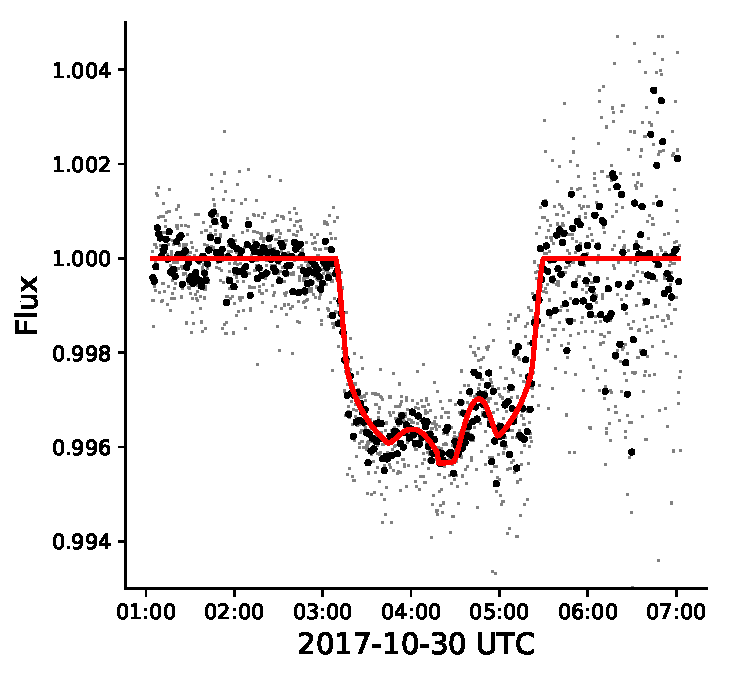
\includegraphics[scale=0.6]{hat11rn/transit_20171030.pdf}}
  \hspace*{.2 in}
  \raisebox{-0.5\height}{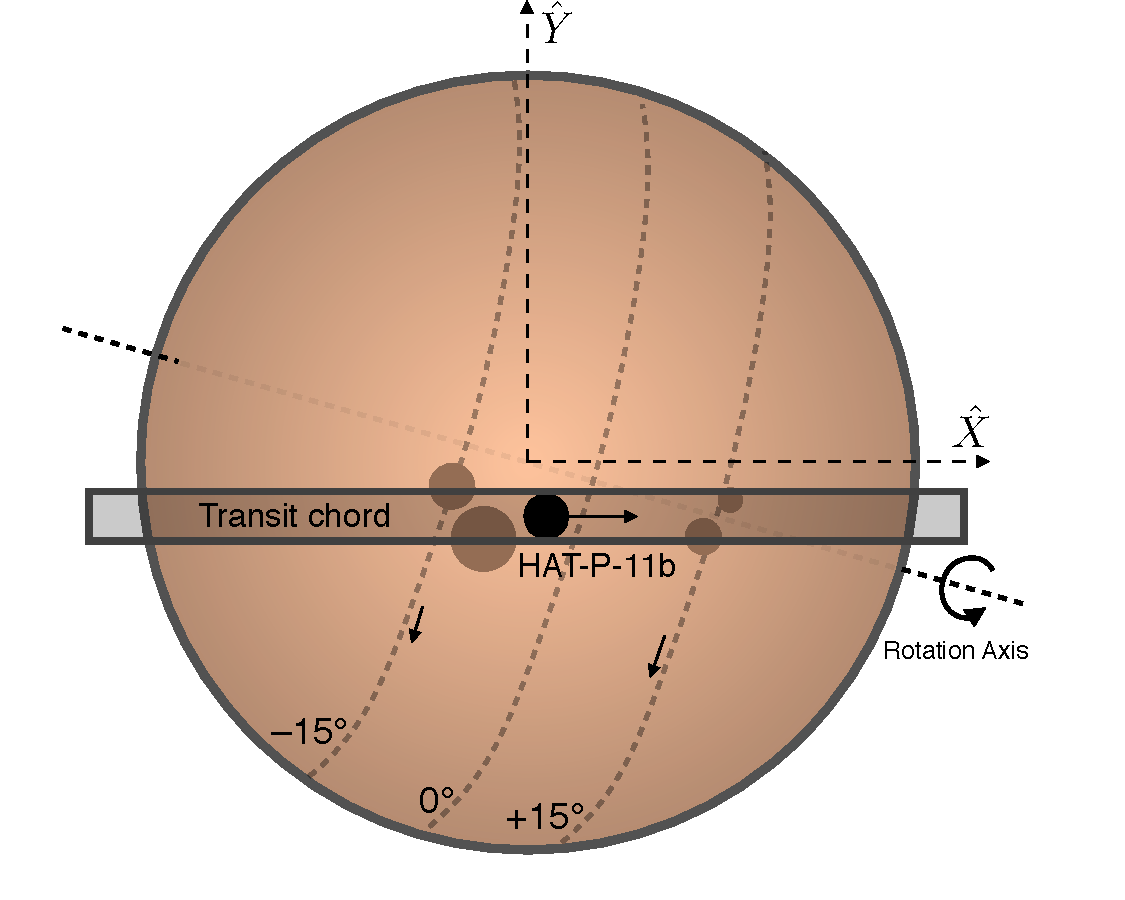
\includegraphics[scale=0.35]{hat11rn/schematic.pdf}}
\end{minipage}
\caption{\textsl{Left}: Transit light curve at 10 second cadence (gray squares) and one minute bins (black circles), with the maximum-likelihood spot model from \texttt{STSP} (red curve). The scatter increases at later times due to high airmass. \textsl{Right}: schematic illustration of a possible spot group configuration consistent with the APO occultation photometry. See Figure 3 of \citet{Morris2017a} for a more detailed explanation of the notation.
\label{fig}}
\end{center}
\end{figure}

% \acknowledgments

% We thank Gudmundur Stefansson and Yiting Li for productive conversations. Based on observations obtained with the APO 3.5-meter telescope, which is owned and operated by ARC.

% \software{\texttt{astropy} \citep{Astropy2013}, \texttt{photutils} \citep{Bradley2016}, \texttt{friedrich} \citep{Morris2017a}, \texttt{astroplan} \citep{astroplan}, STSP \citep{Hebb2018}, \texttt{astroscrappy} \citep{astroscrappy}}

%\facility{APO/ARC 3.5m}

%\bibliography{bibliography.bib}
% \begin{thebibliography}{}
% \expandafter\ifx\csname natexlab\endcsname\relax\def\natexlab#1{#1}\fi
% \providecommand{\url}[1]{\href{#1}{#1}}

% \bibitem[{{Astropy Collaboration} {et~al.}(2013){Astropy Collaboration},
%   {Robitaille}, {Tollerud}, {Greenfield}, {Droettboom}, {Bray}, {Aldcroft},
%   {Davis}, {Ginsburg}, {Price-Whelan}, {Kerzendorf}, {Conley}, {Crighton},
%   {Barbary}, {Muna}, {Ferguson}, {Grollier}, {Parikh}, {Nair}, {Unther},
%   {Deil}, {Woillez}, {Conseil}, {Kramer}, {Turner}, {Singer}, {Fox}, {Weaver},
%   {Zabalza}, {Edwards}, {Azalee Bostroem}, {Burke}, {Casey}, {Crawford},
%   {Dencheva}, {Ely}, {Jenness}, {Labrie}, {Lian Lim}, {Pierfederici},
%   {Pontzen}, {Ptak}, {Refsdal}, {Servillat}, \& {Streicher}}]{Astropy2013}
% {Astropy Collaboration}, {Robitaille}, T.~P., {Tollerud}, E.~J., {et~al.} 2013,
%   \aap, 558, A33

% \bibitem[{{Bakos} {et~al.}(2010){Bakos}, {Torres}, {P{\'a}l}, {Hartman},
%   {Kov{\'a}cs}, {Noyes}, {Latham}, {Sasselov}, {Sip{\H o}cz}, {Esquerdo},
%   {Fischer}, {Johnson}, {Marcy}, {Butler}, {Isaacson}, {Howard}, {Vogt},
%   {Kov{\'a}cs}, {Fernandez}, {Mo{\'o}r}, {Stefanik}, {L{\'a}z{\'a}r}, {Papp},
%   \& {S{\'a}ri}}]{Bakos2010}
% {Bakos}, G.~{\'A}., {Torres}, G., {P{\'a}l}, A., {et~al.} 2010, \apj, 710, 1724

% \bibitem[{{Bradley} {et~al.}(2016){Bradley}, {Sipocz}, {Robitaille},
%   {Tollerud}, {Deil}, {Vin{\'{\i}}cius}, {Barbary}, {G{\"u}nther}, {Bostroem},
%   {Droettboom}, {Bray}, {Bratholm}, {Pickering}, {Craig}, {Pascual}, {Greco},
%   {Donath}, {Kerzendorf}, {Littlefair}, {Barentsen}, {D'Eugenio}, \&
%   {Weaver}}]{Bradley2016}
% {Bradley}, L., {Sipocz}, B., {Robitaille}, T., {et~al.} 2016, {Photutils:
%   Photometry tools}, Astrophysics Source Code Library, , , ascl:1609.011

% \bibitem[{{Hebb} {et~al.}(2018){Hebb}, {Rohn}, \& {collaborators}}]{Hebb2018}
% {Hebb}, L., {Rohn}, G., D.~J. R. A. M. B.~M., \& {collaborators}. 2018

% \bibitem[{{Huehnerhoff} {et~al.}(2016){Huehnerhoff}, {Ketzeback}, {Bradley},
%   {Dembicky}, {Doughty}, {Hawley}, {Johnson}, {Klaene}, {Leon}, {McMillan},
%   {Owen}, {Sayres}, {Sheen}, \& {Shugart}}]{Huehnerhoff2016}
% {Huehnerhoff}, J., {Ketzeback}, W., {Bradley}, A., {et~al.} 2016, in \procspie,
%   Vol. 9908, Ground-based and Airborne Instrumentation for Astronomy VI, 99085H

% \bibitem[{{Morris} {et~al.}(2018){Morris}, {Agol}, \& {Hawley}}]{zwasa}
% {Morris}, B.~M., {Agol}, E., \& {Hawley}, S.~L. 2018, RNAAS

% \bibitem[{{Morris} {et~al.}(2017{\natexlab{a}}){Morris}, {Hebb}, {Davenport},
%   {Rohn}, \& {Hawley}}]{Morris2017a}
% {Morris}, B.~M., {Hebb}, L., {Davenport}, J.~R.~A., {Rohn}, G., \& {Hawley},
%   S.~L. 2017{\natexlab{a}}, \apj, 846, 99

% \bibitem[{{Morris} {et~al.}(2017{\natexlab{b}}){Morris}, {Hawley}, {Hebb},
%   {Sakari}, {Davenport}, {Isaacson}, {Howard}, {Montet}, \&
%   {Agol}}]{Morris2017b}
% {Morris}, B.~M., {Hawley}, S.~L., {Hebb}, L., {et~al.} 2017{\natexlab{b}},
%   \apj, 848, 58

% \bibitem[{{Morris} {et~al.}(2017{\natexlab{c}}){Morris}, {Tollerud}, {Sipocz},
%   {Deil}, {Douglas}, {Berlanga Medina}, {Vyhmeister}, {Smith}, {Littlefair},
%   {Price-Whelan}, {Gee}, \& {Jeschke}}]{astroplan}
% {Morris}, B.~M., {Tollerud}, E., {Sipocz}, B., {et~al.} 2017{\natexlab{c}},
%   ArXiv e-prints, arXiv:1712.09631

% \bibitem[{{Sanchis-Ojeda} \& {Winn}(2011)}]{sanchis-ojeda2011}
% {Sanchis-Ojeda}, R., \& {Winn}, J.~N. 2011, \apj, 743, 61

% \bibitem[{{Solanki}(2003)}]{Solanki2003}
% {Solanki}, S.~K. 2003, \aapr, 11, 153

% \bibitem[{{Stefansson} {et~al.}(2017){Stefansson}, {Mahadevan}, {Hebb},
%   {Wisniewski}, {Huehnerhoff}, {Morris}, {Halverson}, {Zhao}, {Wright},
%   {O'rourke}, {Knutson}, {Hawley}, {Kanodia}, {Li}, {Hagen}, {Liu}, {Beatty},
%   {Bender}, {Robertson}, {Dembicky}, {Gray}, {Ketzeback}, {McMillan}, \&
%   {Rudyk}}]{Stefansson2017}
% {Stefansson}, G., {Mahadevan}, S., {Hebb}, L., {et~al.} 2017, \apj, 848, 9

% \bibitem[{{van Dokkum} {et~al.}(2012){van Dokkum}, {Bloom}, \&
%   {Tewes}}]{astroscrappy}
% {van Dokkum}, P.~G., {Bloom}, J., \& {Tewes}, M. 2012, {L.A.Cosmic: Laplacian
%   Cosmic Ray Identification}, Astrophysics Source Code Library, , ,
%   ascl:1207.005

% \end{thebibliography}

% \end{document}


\chapter{The Chromospheric Activity of HAT-P-11: an Unusually Active, Planet-hosting K Dwarf}

% \documentclass[iop]{emulateapj}
% \documentclass[preprint2]{aastex61}
%\documentclass[preprint2]{aastex61}
%
%\usepackage{natbib}
%\bibliographystyle{humannat}
%
% \newcommand{\stsp}{\texttt{STSP}\xspace}
% \newcommand{\kepler}{\textit{Kepler}\xspace}
\newcommand{\rprime}{$R^\prime_{HK}$\xspace}

%
%%@arxiver{s-index_hat11.pdf,cks_activity.pdf}
%
%\shorttitle{Chromospheric activity of HAT-P-11}
%\shortauthors{Morris et al.}
%
%\begin{document}
%
%\title{Chromospheric Activity of HAT-P-11: an Unusually Active Planet-Hosting K Star}
%
%\author{Brett M. Morris}
%\affiliation{Astronomy Department, University of Washington, Seattle, WA 98195, USA}
%                 
%\author{Suzanne L. Hawley}
%\affiliation{Astronomy Department, University of Washington, Seattle, WA 98195, USA}
%
%\author{Leslie Hebb}
%\affiliation{Physics Department, Hobart and William Smith Colleges, 
%                 Geneva, NY 14456, USA}
%                 
%\author{Charli Sakari}
%\affiliation{Astronomy Department, University of Washington, Seattle, WA 98195, USA}
%
%\author{James. R. A. Davenport}
%\affiliation{Department of Physics \& Astronomy, Western Washington University, 516 High St., Bellingham, WA 98225, USA}
%\affiliation{NSF Astronomy and Astrophysics Postdoctoral Fellow}
%
%\author{Howard Isaacson}
%\affiliation{Department of Astronomy, UC Berkeley, Berkeley, CA 94720, USA}
%
%\author{Andrew W. Howard}
%\affiliation{Department of Astrophysics, California Institute of Technology, MC 249-17, Pasadena, CA 91125, USA}
%
%\author{Benjamin T. Montet}
%\affiliation{Department of Astronomy and Astrophysics, University of Chicago, 5640 S. Ellis Avenue, Chicago, IL 60637, USA}
%\affiliation{NASA Sagan Fellow}
%
%\author{Eric Agol}
%\affiliation{Astronomy Department, University of Washington, Seattle, WA 98195, USA}
%
%\email{bmmorris@uw.edu}

% \begin{abstract}
% \kepler\ photometry of the hot Neptune host star HAT-P-11 suggests that its spot latitude distribution is comparable to the Sun's near solar maximum. We search for evidence of an activity cycle in the CaII H \& K chromospheric emission $S$-index with archival Keck/HIRES spectra and observations from the echelle spectrograph on the ARC 3.5 m Telescope at APO. The chromospheric emission of HAT-P-11 is consistent with a $\gtrsim 10$ year activity cycle, which plateaued near maximum during the \kepler\ mission. In the cycle that we observed, the star seemed to spend more time near active maximum than minimum. We compare the $\log R^\prime_{HK}$ normalized chromospheric emission index of HAT-P-11 with other stars. HAT-P-11 has unusually strong chromospheric emission compared to planet-hosting stars of similar effective temperature and rotation period, perhaps due to tides raised by its planet.
% \end{abstract}

%\keywords{Chromospheric activity, stellar dynamo, activity cycles, S-index, tides}

\section{Introduction}

The K4 dwarf HAT-P-11 bears many spots on its surface, despite its 29 day rotation period. \citet{Morris2017} used \kepler\ photometry to measure spot sizes and positions during transits of its hot Neptune with a nearly polar orbit. They showed that the spots cover $\sim$100x more surface area on HAT-P-11 than sunspots cover on the Sun, and that the spots cluster into active latitudes similar to the solar active latitudes near activity maximum. The analysis by \citet{Morris2017} was limited in time to the four years of \kepler\ photometry, preventing the detection of activity evolution throughout the stellar activity cycle. The transit photometry also restricted their analysis to spots within the transit chord, which covers only 6\% of the observer-facing stellar hemisphere per transit. 

High resolution spectroscopy is a complementary means of quantifying the disk-integrated activity of HAT-P-11 on long timescales. Emission in the cores of the CaII H \& K features is generated in the chromosphere over active regions. CaII H \& K emission is typically measured as the flux in the emission features normalized by two pseudocontinuum regions on either side of the absorption features, called the $S$-index. The $S$ and related \rprime\ indices of solar-like stars has been studied over many years and across spectral types and ages \citep{Wilson1978, Noyes1984, Duncan1991, Baliunas1995}. CaII emission generally declines with age \citep{Skumanich1972} -- with a large intrinsic variance driven by the rotation of active regions into and out of view, and stellar activity cycles \citep[see review by][]{Hall2008}.

Here we measure the $S$-index of HAT-P-11, and put the activity of HAT-P-11 into context among stars of similar spectral type and age by calculating \rprime. In Section~\ref{sec:sindex} we present spectroscopy from Keck/HIRES and Apache Point Observatory (APO) ARC 3.5 m Telescope from 2008-2017 and find evidence for an activity cycle. We compare the activity cycle observed in spectroscopy with the total stellar brightness in the \kepler\ band from full-frame image photometry in Section~\ref{sec:ffi}. In Section~\ref{sec:cks} we investigate whether or not the abundant activity of HAT-P-11 is ``normal'' among stars of similar age and spectral type.

\section{Observations of the $S$-index} \label{sec:sindex}

We can search for the activity cycle of HAT-P-11 if we combine observations from Keck/HIRES and recent observations from the Astrophysical Research Consortium (ARC) 3.5 m Telescope at APO. However, the definition of the $S$-index has the unfortunate property that its value varies from one instrument to the next for the same intrinsic flux. Therefore $S$-index measurements must be calibrated against the stars observed in the Mount Wilson Observatory (MWO) sample before spectra from different observatories can be compared. In Section~\ref{sec:s_apo} we calibrate the linear correction for the $S$-index measured by the ARC Echelle Spectrograph (ARCES) at APO, and in Section~\ref{sec:s_h11} we combine the recent APO spectra with archival Keck/HIRES spectra to span nine years of observations.

\subsection{Calibrating the $S$-index for APO} \label{sec:s_apo}

We reduce the raw ARCES spectra with \texttt{IRAF} methods to subtract biases, remove cosmic rays, normalize by the flat field, and do the wavelength calibration with exposures of a thorium-argon lamp\footnote{An ARCES data reduction manual by J. Thorburn is available at \url{http://astronomy.nmsu.edu:8000/apo-wiki/attachment/wiki/ARCES/Thorburn_ARCES_manual.pdf}}. We fit the spectrum of an early-type star with a high-order polynomial to measure the blaze function, and we divide the spectra of HAT-P-11 and the MWO stars by the polynomial fit to normalize each spectral order.

Next the normalized spectra must be shifted in wavelength into the rest-frame by removing their radial velocities. We remove the radial velocity by maximizing the cross-correlation of the ARCES spectra with PHOENIX model atmosphere spectra \citep{Husser2013}.

\begin{figure}
\centering
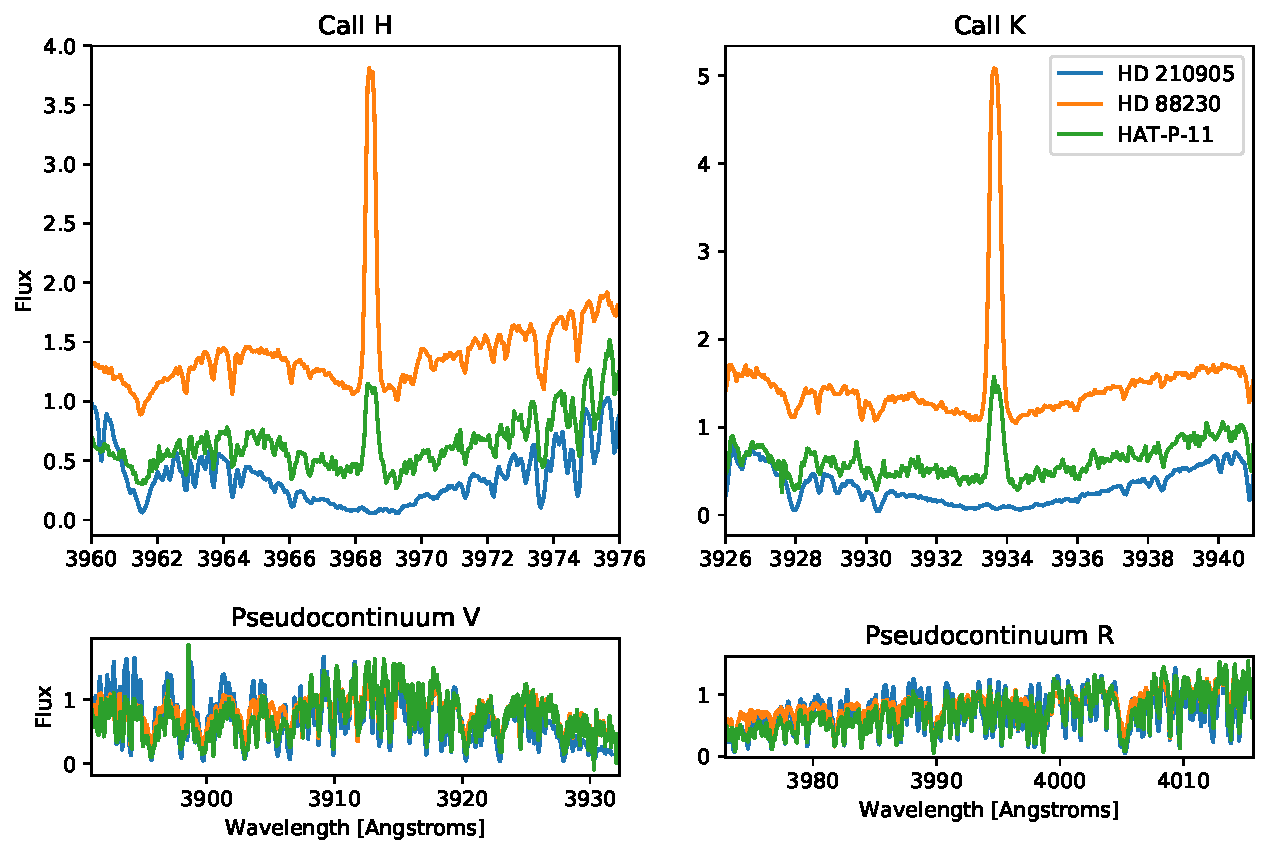
\includegraphics[scale=0.7]{sindex/example_spectra.pdf}
\caption{Spectra of two CaII H \& K calibration targets on the high and low activity ends, and HAT-P-11 in the middle.}
\label{fig:examplespectra}
\end{figure}

To calibrate the ARCES spectra, we follow the calibration procedure developed in \citet{Isaacson2010} for HIRES. We collect 51 spectra of 30 stars in the \citet{Duncan1991} MWO sample with the ARC 3.5 m Telescope at APO and the ARCES spectrograph, including 22 K stars, 7 G stars and one M star -- see Figure~\ref{fig:examplespectra} for example spectra. 

We measure the $S$-index for these stars by taking the sum of the flux in the cores of the $H$ and $K$ features at 3968.47 \AA\ and 3933.66 \AA, weighted with a triangular weighting function with FWHM=$1.09$\AA. We normalize the weighted emission by the flux in pseudocontinuum regions $R$ and $V$, which are 20 \AA-wide bands centered on 3900 and 4000 \AA, respectively. Then $S$ on the MWO-calibrated scale is 
\begin{eqnarray}
S_{APO} &=& \frac{a~H + b~K}{c~R + d~V} \\
S_{MWO} &=& C_1 S_{APO} + C_2, \label{eqn:s_ind}
\end{eqnarray}
where $a,~b,~c,~d, ~C_1$ and $C_2$ are parameters that can be tuned to make ARCES $S$-indices match the scale of $S_{MWO}$ \citep{Duncan1991}. Following the example of \citet{Isaacson2010}, we chose values of $a,b,c,d$ so that $S$ has roughly equal flux contributions from the $H$ and $K$ emission lines, and roughly equal flux from the $R$ and $V$ psuedocontinuum regions in the APO spectra. Thus we set $a = c = 1$, and we choose $b=2$ and $d=1$, so that $H \sim b~K$ and $K \sim d~V$. 

Since $S$ varies over time for each star in the sample, the linear correlation between the $S_{APO}$ and $S_{MWO}$ will have some intrinsic spread. To incorporate this into our model, we adopt the $\left< S \right>$ and the standard deviation of $S$ from \citet{Duncan1991} as the measurement and uncertainty of the MWO values. We solve for the constants $C_1$ and $C_2$ and their uncertainties with Markov Chain Monte Carlo (MCMC) \citep{Goodman2010, Foreman-Mackey2013}; the results are shown in Figure~\ref{fig:calib}. We find $C_1 = 21.26_{-0.83}^{+0.99}$ and $C_2 = 0.009_{-0.009}^{+0.011}$. The $S$-indices for each target are enumerated in Table~\ref{tab:cals}. The software tools used to calculate calibrated $S$-indices with spectra from ARCES are publicly available \footnote{\url{https://doi.org/10.5281/zenodo.886629}}.

\begin{figure}
\begin{center}
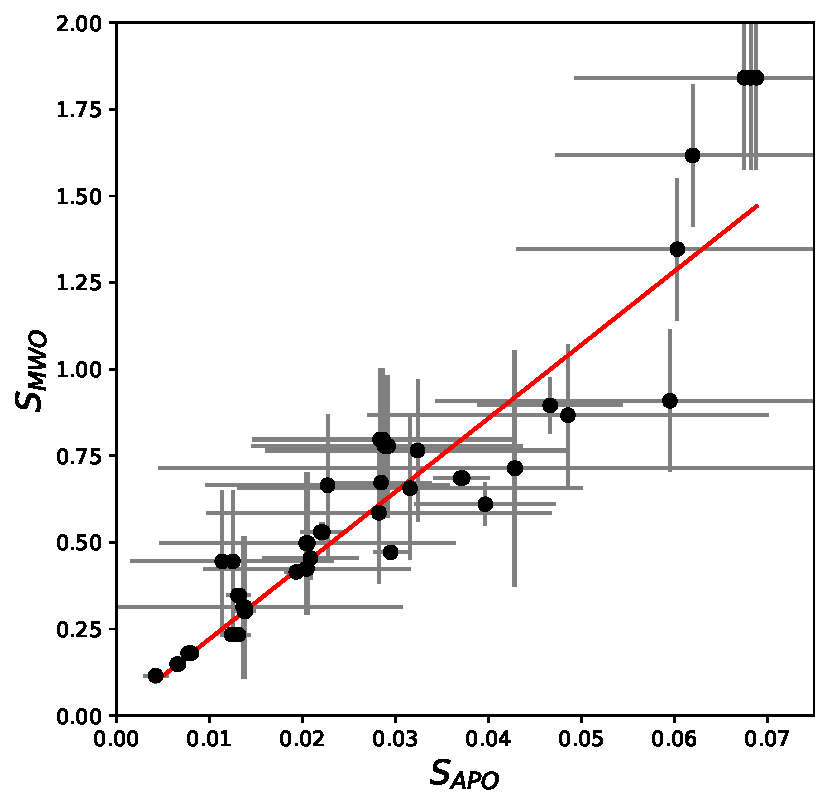
\includegraphics[scale=0.8]{sindex/s-index_calibration.pdf}
\caption{We calibrate the $S$-index measured with the APO echelle spectra against previous measurements from Mount Wilson Observatory (MWO) \citep{Duncan1991}. The large uncertainties in the MWO measurements are a result of the intrinsic activity variation of each star, and the uncertainties of the APO observations correspond to the measurement uncertainties.}
\end{center}
\label{fig:calib}
\end{figure}

\subsection{The $S$-index of HAT-P-11} \label{sec:s_h11}

\begin{figure}
\centering
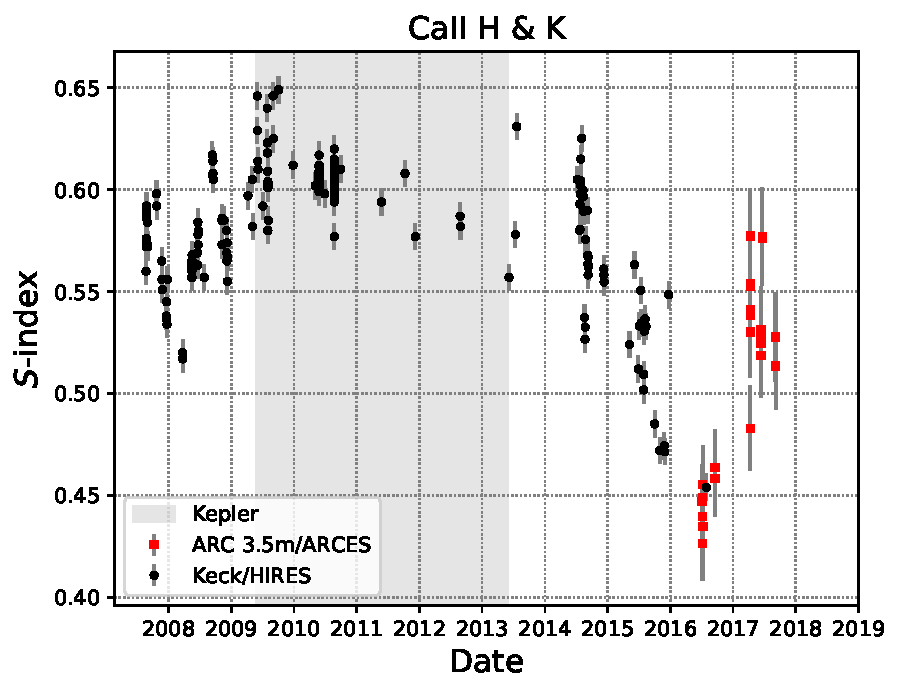
\includegraphics[scale=0.7]{sindex/s-index_hat11.pdf}
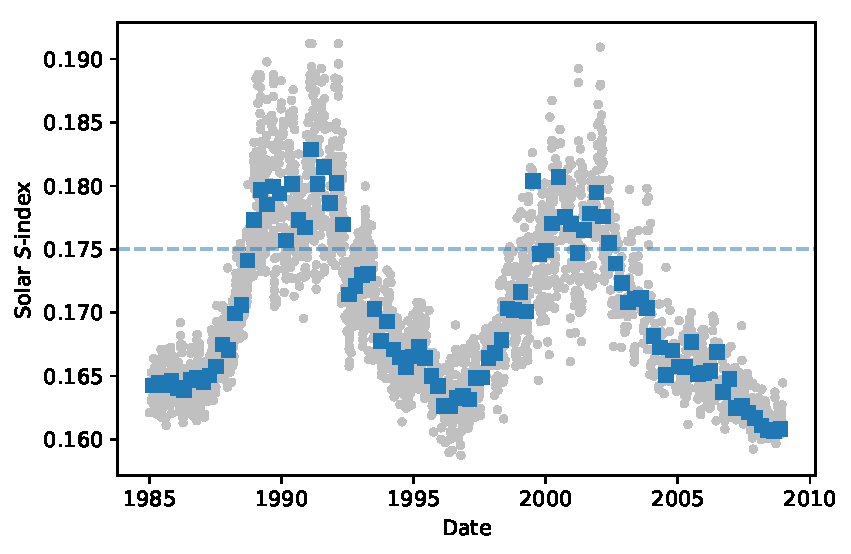
\includegraphics[scale=0.7]{sindex/solar_sind.pdf}
\caption{\textit{Upper:} $S$-index of HAT-P-11 over time with archival Keck/HIRES spectra and calibrated APO spectra from this work. We see evidence for an activity cycle with period $\sim$10 years or more. \textit{Lower:} the $S$-index of the Sun, from the National Solar Observatory (NSO) Integrated Sunlight Spectrometer (ISS) on the Synoptic Optical Long-term Investigations of the Sun (SOLIS) telescope. We convert the ISS CaII $K$ line fluxes to $S$-indices with Eqns.~5 and 12 of \citet{Egeland2017}. If we have observed nearly one complete activity cycle of HAT-P-11, it appears that HAT-P-11 spends a longer fraction of the cycle near activity maximum than the Sun does.}
\label{fig:activity_cycle}
\end{figure}

With the transformation computed in the previous section, we can compare the APO $S$-index measurements with those from the archival Keck/HIRES spectra. HAT-P-11 was the target of several Keck/HIRES programs since the planet's discovery, with the aims of measuring the Rossiter-McLaughlin effect and searching for a third body\footnote{We use archival spectra from program PIs: Bakos, D.~Bayliss, Beichman, Borucki, P.~Butler, D.~Fischer, Ford, Fortney, J.~Fuller, Gaidos, Hillenbrand, Howard, J~Johnson, Knutson, Mandushev, Marcy, Rogers, Sanchis-Ojeda, S.~Vogt}. We measure $S$-indices from these observations with the HIRES activity pipeline described in \citet{Isaacson2010}. A complete description of the HIRES pipeline developed for these measurements is beyond the scope of this paper; we refer the reader to \citet{Isaacson2010} for the full description. The result is an unevenly-sampled series of 239 $S$ measurements spanning 2007-2016, with typical $S/N \sim 20$. 

Figure~\ref{fig:activity_cycle} shows the $S$-index of HAT-P-11 between 2008-2017, including both the APO and Keck spectra. The APO $S$-indices are enumerated in Table~\ref{tab:sind}.The black circles are measurements from Keck/HIRES, and the red circles are measurements from APO. The chromospheric activity of HAT-P-11 appears to ramp up in the years preceding the \kepler\ mission, stabilize near a maximum throughout the \kepler\ years from 2009-2014, and then decline rapidly from 2014-2016 before rising at a similar rate through the present. 

Activity indices like $S$ vary on two timescales -- one driven by the rotation period of the star (29.2 d) as active regions rotate into and out of view, and the longer timescale throughout the activity cycle. It appears from this limited time series that HAT-P-11 may have entered activity maximum near the beginning of the \kepler\ observations. It is interesting to note that \citet{Morris2017} found that the starspots of HAT-P-11 are distributed in active latitudes centered on $\bar{\ell} = 16 \pm 1^\circ$, similar to the distribution of sunspots near solar activity maximum. The $S$-index appears to corroborate that if HAT-P-11's activity cycle is similar to the Sun's, it was at active maximum during the \kepler\ years.

Further spectroscopic monitoring will be required to determine the period of the activity cycle of HAT-P-11. During the summer of 2017, we measure $\left< S\right>_{2017} = 0.54 \pm 0.04$, still less than the earliest available measurements from the summer of 2007 $\left< S\right>_{2007} = 0.569 \pm 0.006$ -- it appears that one complete activity cycle has not yet elapsed. This gives a lower limit on the activity cycle period of $\sim 10$ years. The solar activity cycle is not perfectly periodic; the mean cycle duration and standard deviation are $10.9 \pm 1.2$ years \citep{Hathaway2002}. This lower limit on the activity cycle of HAT-P-11 observed thus far is longer than some solar activity cycles, but not longer than the mean. In principle one could attempt to measure the period of HAT-P-11's cycle by invoking empirical models of $S$ inspired by the solar activity cycle. However, as we will discuss below, HAT-P-11's $S$-index distribution with time departs from the typical $S$ distribution of the Sun -- HAT-P-11 spends more time near active maximum than minimum. Therefore we can only constrain a lower limit on the period with the observations thus far, and refrain from attempting to fit for the cycle period. 

The activity minimum of HAT-P-11 was short compared to its maximum. We note the marked difference between HAT-P-11 and the Sun in this respect in Figure~\ref{fig:activity_cycle}. Since we have not yet measured a full activity cycle of HAT-P-11 and the time sampling is very uneven, it is difficult to make concrete statements about the true duration of its maximum or minimum. One quantity that might be robust against these biases is the fraction of the activity cycle spent above or below the mean of $S_{min}$ and $S_{max}$, assuming the minimum and maximum observed $S$ are close to the true minimum and maximum of $S$ throughout the cycle. The Sun spends 25\% of the cycle above $0.5 (S_{min} + S_{max}) = 0.174$. The same quantity for HAT-P-11 is $0.5 (S_{min} + S_{max}) = 0.53$, and its $S$ was above that value from around or before 2008 until mid-2015, and stayed below that value until mid-2017. It appears that HAT-P-11 spent 63\% of its cycle above the mean of $S_{min}$ and $S_{max}$, assuming an $\sim 11$ year cycle. 

If HAT-P-11 has an $\sim 11$ year activity cycle, it falls in a sparse region of rotation period-cycle period parameter space. \citet{Bohm-Vitense2007} showed that stars typically fall into one of two categories: the young, active $A$-sequence, and old, inactive $I$-sequence (see \citealt{Bohm-Vitense2007} Fig.~1). $A$-sequence stars typically have ratios of cycle periods to rotation periods $P_{cyc}/P_{rot} \sim 360$, and $I$-sequence stars have $P_{cyc}/P_{rot} \sim 80$.  The Sun is a notable outlier residing in between the sequences with $P_{cyc}/P_{rot} \sim 160$. If HAT-P-11's activity cycle is roughly $\sim 11$ years, it is interesting to note that it has $P_{cyc}/P_{rot} \sim 139$, and it falls between the $A$ and $I$ sequences, like the Sun.

The APO spectra in Figure~\ref{fig:h} demonstrate that the activity has increased significantly in just the last two years. If we assume the cycle has a period of $\sim$11 years, we expect the next maximum to begin near 2019-2020. We predict that TESS photometry of HAT-P-11 will show spot occultations similar to those observed during the \kepler\ mission.

\begin{figure}
\begin{center}
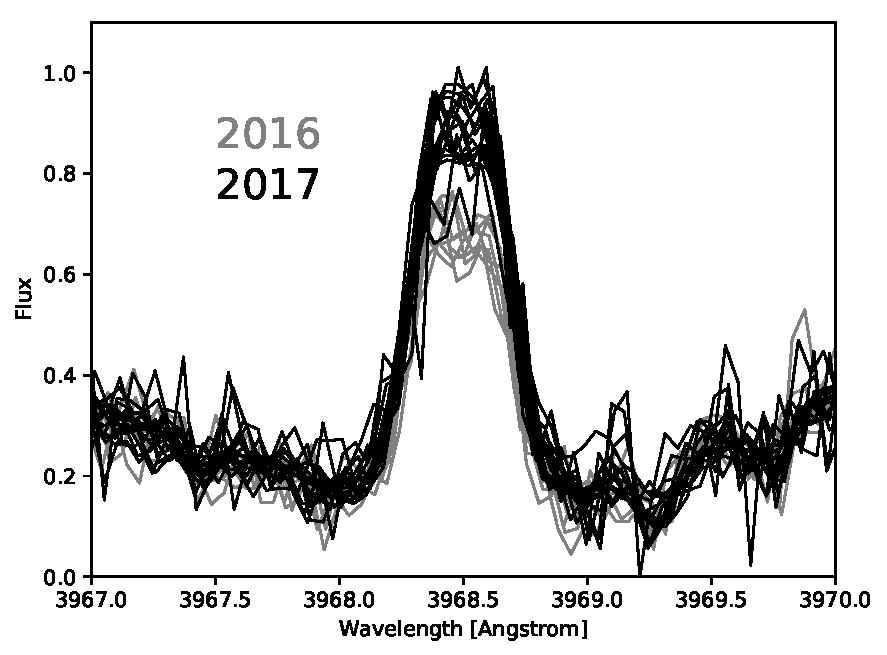
\includegraphics[scale=0.8]{sindex/close_up_h.pdf}
\end{center}
\caption{The CaII H feature of HAT-P-11 shows clear evolution towards more activity from 2016 to 2017 in the APO spectra. It appears that the activity may be approaching its maximal level as of mid-2017.}
\label{fig:h}
\end{figure}

\section{\kepler\ Full-frame image photometry} \label{sec:ffi}

\citet{Montet2017} searched for long term variability of \kepler\ targets in photometry from the full-frame images (FFIs). These were special exposures where the entire \kepler\ detector was read-out, whereas the short and long cadence photometry from \kepler\ was only telemetered for a small subset of the pixels. There were eight FFIs in 2009 during commissioning, and then approximately one per month for the remainder of the mission.

We use HAT-P-11 as a test-case for the reliability of long-term trends in FFI photometry, see Figure~\ref{fig:ffi}. The FFI photometry shows that the flux of HAT-P-11 varied by $\sim 2\%$ from 2009-2013 without a significant secular trend. The scatter in the FFI photometry is consistent with the scatter in the short-cadence SAP fluxes due to rotational variability of the star. Note that one should only compare the global scatter of the FFI and SAP fluxes to one another, and one should not expect the SAP light curve to perfectly intersect with the SAP measurements, since the SAP fluxes shown in Figure~\ref{fig:ffi} are normalized by the median flux of each quarter, and the FFI fluxes are normalized by the median flux over all FFIs. 

The $S$-index in Figure~\ref{fig:activity_cycle} indicates that HAT-P-11 had nearly uniform chromospheric emission throughout the years of the \kepler\ mission. Both the \kepler\ photometry and $S$-index are consistent with an active maximum period from 2009-2013.

The long term photometric variability of most Sun-like stars with rotation periods of 29 d is dominated by bright faculae \citep{Montet2017}. Future space-based photometry missions could therefore expect to measure a small dimming of the star during its short activity minimum.

\begin{figure}
\begin{center}
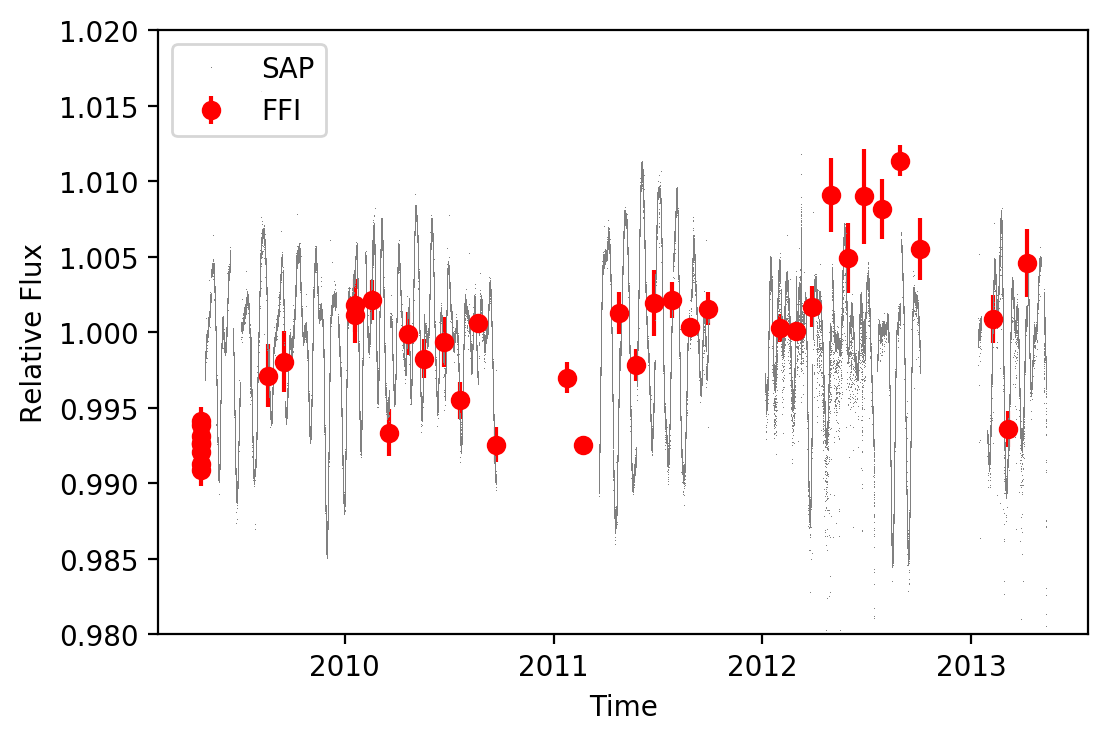
\includegraphics[scale=0.8]{sindex/ffi.png}
\end{center}
\caption{Full-frame image photometry of HAT-P-11 (red circles) and \kepler\ SAP one minute cadence fluxes (gray). \citet{Montet2017} searched for evidence of stellar activity cycles in the full-frame image (FFI) photometry. The $S$-index was near maximum throughout the \kepler\ mission, so we expect the FFI photometry to show scatter consistent with the 2\% rotational modulation in the \kepler\ short-cadence light curve. The FFI photometry indeed show scatter consistent with the rotational variability, without a significant secular trend.}
\label{fig:ffi}
\end{figure}

\section{HAT-P-11 in context} \label{sec:cks}

\subsection{Comparison to stars of similar color} \label{sec:mittag}

Is the chromospheric activity of HAT-P-11 typical for K4 dwarfs? The photometric analysis by \citet{Morris2017} can't be reproduced for many other \kepler\ stars. HAT-P-11 is exceptionally bright ($V=9.59$), and the highly inclined orbit of its planet reveals the latitude distribution of spots during transit events. Since very few similar targets are available for comparison in the \kepler\ sample, we seek to compare the spectrum of HAT-P-11 to spectra of other stars.

The $S$-index varies with stellar effective temperature, so the large $S$ of HAT-P-11 compared to the Sun does not imply that HAT-P-11 has more chromospheric activity than the Sun. The \rprime\ index is often used instead to compare activity levels across the main sequence, by normalizing the flux in the CaII H \& K emission features by the basal flux from the photosphere \citep{Noyes1984}. For stars of any effective temperature, \rprime\ increases with chromospheric activity.

We compute the \rprime\ index for a large sample of main sequence stars, following the procedure of \citet{Mittag2013}. We gathered published $S$-indices from \citet{Duncan1991}, \citet{Wright2004} and \citet{Isaacson2010}. As in \citet{Mittag2013}, we select only main sequence stars with color and absolute magnitude cuts using Hipparcos parallaxes \citep{Perryman1997}, yielding a sample of 4677 main sequence stars with measured $S$-indices. We then solve for \rprime\ for each star. We also compute \rprime\ for HAT-P-11 using its mean $\left < S \right> = 0.58 \pm 0.04$.

\begin{figure}
\begin{center}
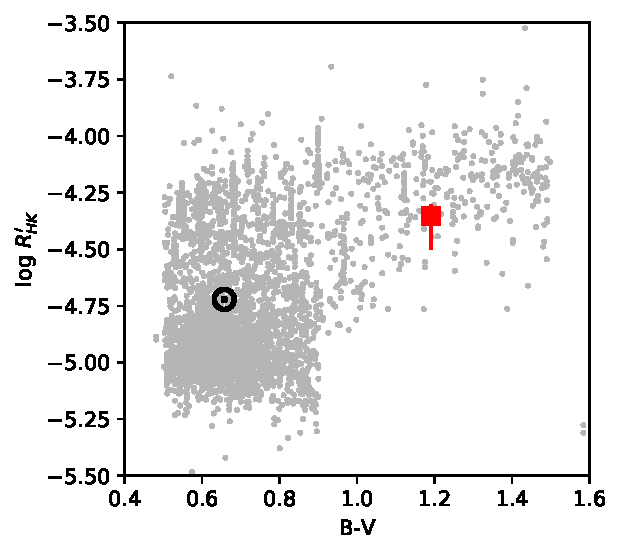
\includegraphics[scale=1]{sindex/rprime.pdf}
\end{center}
\caption{The \rprime\ index of HAT-P-11 (red square) among other main sequence stars (circles). The Sun is represented by the black ``$\odot$'' symbol, and resides on the the inactive branch of bluer stars. The distribution of \rprime\ at a given $B-V$ color is dominated by variation with age. Dwarfs with $B-V > 1$ typically have more active chromospheres than dwarfs with $B-V <1$. The errorbars on the square representing HAT-P-11 denote the minimum and maximum \rprime\ given the complete range of observed $S$ values throughout the activity cycle.}
\label{fig:rprime_ms}
\end{figure}

The \rprime\ index for each star in the literature is shown in Figure~\ref{fig:rprime_ms}. The characteristic rise in chromospheric activity for later type stars is visible in the right half of the figure. HAT-P-11 is the red square with $B-V = 1.19$ and $\log R^\prime_{HK} = -4.35$ (evaluated for $\left<S\right>$). The Sun is represented with the $\odot$ symbol and resides in the inactive sequence, blueward of HAT-P-11. 

HAT-P-11 has typical chromospheric activity among field stars of similar color. It lies near the lower envelope of \rprime\ at $B-V\sim1.2$, which one might expect given its rotation period $P_{rot} = 29.2$ d since \rprime\ declines with increasing age and rotation period \citep{Noyes1984}. HAT-P-11 also hosts a close-in planet which one might speculate could affect its activity, and in general we don't know the planet occurrence frequency in this sample of stars. As a result, it is perhaps more interesting to compare the chromospheric activity of HAT-P-11 to planet-hosting stars of similar color \textit{and} age.

\subsection{Comparison to planet hosts of similar color and age}

\begin{figure}
\begin{center}
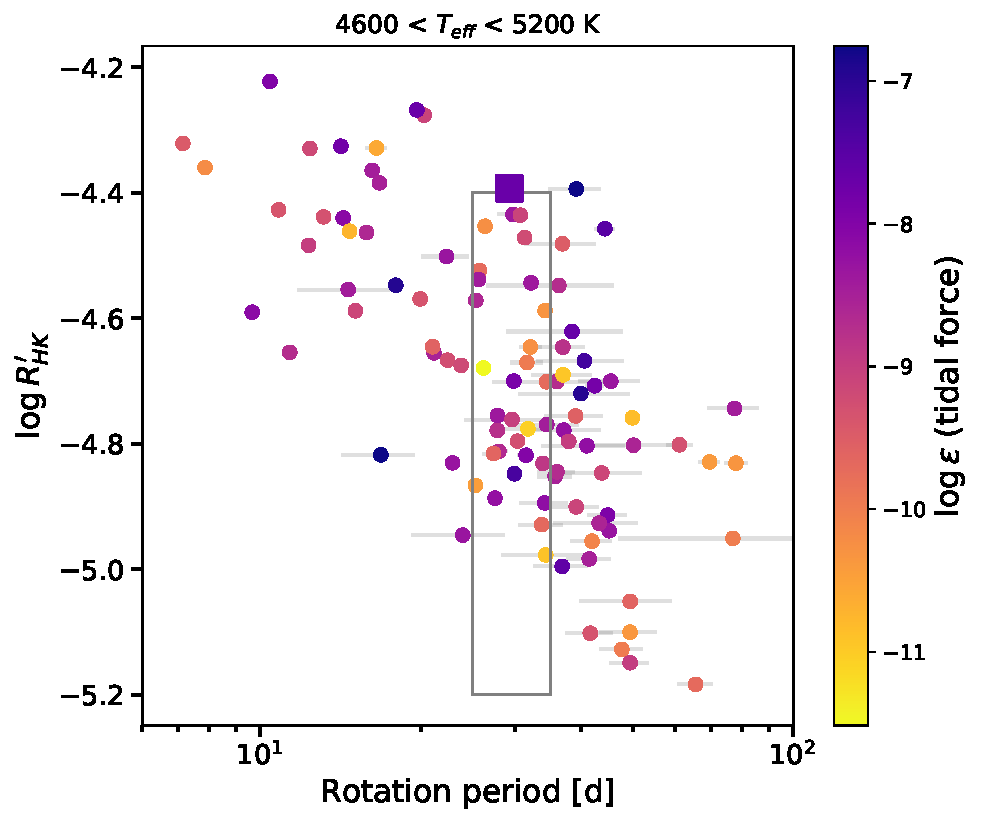
\includegraphics[scale=0.8]{sindex/cks_activity.pdf}
\end{center}
\caption{The \rprime\ index of HAT-P-11 (big square) among other main sequence planet-hosting stars (circles). HAT-P-11 is among the most active planet-hosting K stars with rotation periods near 30 d -- its \rprime\ is similar to the median \rprime\ for stars with rotation periods near $\sim 15$ days.}
\label{fig:cks_activity}
\end{figure}

Is the chromospheric activity of HAT-P-11 typical for planet-hosting K stars with long rotation periods? We build a sample of stars with similar effective temperatures to HAT-P-11 from the California-Kepler Survey (CKS), in which \citet{Petigura2017} published Keck/HIRES spectra and \citet{Johnson2017} published precise stellar parameters for 1305 planet-hosting \kepler\ stars.  We gather the CKS spectra of 107 planet-hosting stars which meet the following criteria: they have (1) effective temperatures in the range $4600 < T_{eff} < 5200$ K \citet{Petigura2017}, bracketing HAT-P-11 at $T_{eff} = 4780 \pm 50$ K \citep{Bakos2010}; (2) innermost planets with orbital periods $<20$ days; and (3) $S/N > 50$, where we approximate $S/N$ by dividing the median flux in the blue spectrum by the median uncertainty in the public CKS spectra.

We replicate the procedure in Section~\ref{sec:s_apo} to calculate $S$-indices for the CKS stars using the HIRES correction coefficients from \citet{Isaacson2010}, and use the relations of \citet{Mittag2013} to compute \rprime\ indices for each star as in Section~\ref{sec:mittag}. We also gather rotation periods for each star from \citet{Mazeh2015}, and we compute the Rossby number for each star with convective turnover times computed from the relations of \citet{Wright2011}.

We are particularly interested in whether or not HAT-P-11 experiences unusual planet-induced tides, which could provide a coupling between the planet's orbit and stellar activity. To quantify the relative tidal force on each star at the seat of stellar activity, the base of the convective zone, we use the simple dimensionless parameter $\epsilon$, 
\begin{equation}
\epsilon = \frac{M_p}{M_\star} \left( \frac{R_c}{a}\right)^3
\end{equation}
where $M_p$ and $M_\star$ are the masses of the planet and star, $R_c$ is the radius of the convective zone, and $a$ is planet's orbital semi-major axis \citep{Ogilvie2014}. The above equation is the ratio of the tidal force of the planet at the base of the convective zone $F_{tide} \propto M_p R_c / a^3$ to the local force of gravity within the star $F_g \propto M_\star / R_c^2$. This simple ratio does not take into account other likely important factors like the stellar obliquity. However, in the vast majority of cases the stellar obliquity is not known, so we continue to investigate tides with the imperfect index $\epsilon$, and discuss the implications of this caveat below.

We evaluate the tidal $\epsilon$ for the innermost planet in each system. We adopt the stellar radii and semi-major axes from the isochrone fits of \citet{Johnson2017}. We estimate the radius of the convective zone for each star by interpolating between the convective zone radii of model stars by \citet{vanSaders2012} of solar metallicity with $4600<T_{eff}<5200$ K. Finally, we adopt the mass measurement for HAT-P-11 b, $M_p=0.081 M_J$ from \citet{Bakos2010}, and estimate the most probable mass for all other planets using the \texttt{forecaster} tool by \citet{Chen2017}, given the measured planetary radii from \citet{Johnson2017}.

We recover the canonical result that \rprime\ generally decreases with rotation rate (or age) in Figure~\ref{fig:cks_activity}. It appears that HAT-P-11 (large square) has more chromospheric activity than other planet-hosting stars of similar rotation periods and effective temperatures. The gray box in Figure~\ref{fig:cks_activity} circumscribes 31 stars with rotation periods $25 < P_{rot} < 35$ d. The median activity level within the box is only 40\% of HAT-P-11's, $\log R^\prime_{HK} = -4.75$.

\subsection{The possible role of tides}

\begin{figure}
\begin{center}
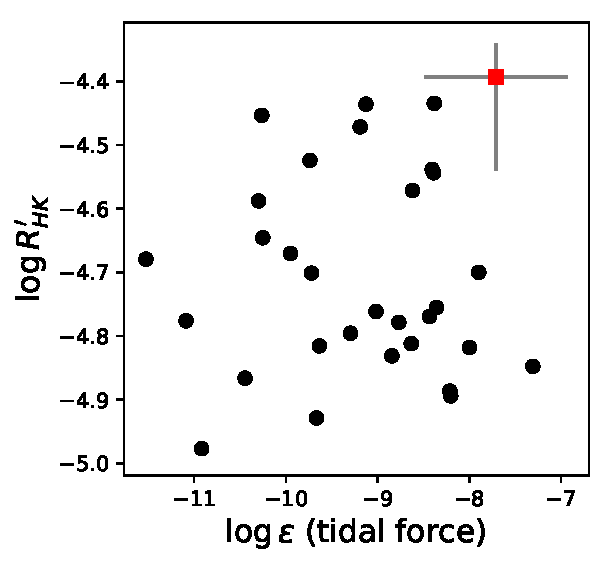
\includegraphics[scale=1]{sindex/tides_rhk.pdf}
\caption{The \rprime\ index for stars within the gray box in Figure~\ref{fig:cks_activity}, with rotation periods $25 < P_{rot} < 35$ d and effective temperatures $4600 < T_{eff} < 5200$ K. HAT-P-11 (red square) has the most activity in this bin, and the second-greatest tidal force on the base of its convective zone. The uncertainty in \rprime\ on HAT-P-11 represent its variation throughout its activity cycle. The uncertainty in $\epsilon$ on HAT-P-11 represents the characteristic uncertainty for all systems, which is dominated by uncertainty in the planet mass-radius relation of \citet{Chen2017}.}
\label{fig:rhk_eps}
\end{center}
\end{figure}

Could the relatively high level of chromospheric activity on HAT-P-11 (for stars with its age and color) be related to the tides raised by the close-in planet? We show the $\epsilon$-\rprime\ distribution of stars with $25 < P_{rot} < 35$ d in Figure~\ref{fig:rhk_eps}. We note that in this range of rotation periods, HAT-P-11 (red square) has the most chromospheric activity and the second-greatest $\epsilon$. However, the lack of  correlation between \rprime\ and $\epsilon$ suggests: (1) the tidal force isn't the only important factor in setting the level of chromospheric activity; and (2) the simple parameterization of $\epsilon$ does not capture all of the relevant physics. 

Significant tides are raised by HAT-P-11 b, even when compared to solar system objects. We can compare it's $\log_{10}\epsilon = -7.7$ with more familiar systems. $\epsilon$ at the base of the solar convective zone due to tides raised by Mercury gives $\log_{10}\epsilon = -13$, much less than any of the systems in Figure~\ref{fig:rhk_eps}. The Earth-Moon system experiences more similar tides with $\log_{10}\epsilon = -7.3$, and the dimensionless tidal force on HAT-P-11 is significantly less than the Jupiter-Io tides, $\log_{10}\epsilon = -6.6$. The tides raised by HAT-P-11 b are significant, and may have non-negligible effects on the interior dynamics of the star.

\subsection{The possible role of stellar obliquity}

Why is there no correlation between tidal force and chromospheric activity in this sample? We investigate the system with the greatest $\epsilon$ in more detail. That system is KOI-1050 with $\log_{10}\epsilon=-7.2$. Its star has mass $M_\star = 0.83 M_\odot$, effective temperature $T_{eff}= 5068$ K and rotation period $P_{rot} = 29.9$ d. It is orbited by planet with radius $R_p = 1.85 R_\oplus$, orbital period $1.27$ d and forecasted mass $M_p = 4.4 M_\oplus$. \rprime\ of KOI-1050 is less than half of HAT-P-11's despite its larger $\epsilon$. 

The dimensionless tidal force $\epsilon$ does not account for the transfer of energy due to obliquity tides -- the result of additional torques in star-planet systems with planetary orbits that are highly misaligned with respect to the stellar spin. The amplitude of energy transfer due to obliquity tides is proportional to $\sin^2 \psi$, where $\psi$ is the angle between the orbital angular moment vector and the stellar spin axis \citep{Wisdom2004}. The high obliquity of HAT-P-11 $\psi = 106^\circ {}^{+15}_{-11}$ suggests that obliquity tides on HAT-P-11 will contribute additional dissipation of orbital energy, which is not reflected by $\epsilon$. Lacking measurements of the obliquity of the other systems in Figure~\ref{fig:rhk_eps} such as KOI-1050, the observations presented here are insufficient to comment on whether or not the high obliquity of HAT-P-11 is responsible for its greater \rprime\ activity index compared to KOI-1050, for example. Future measurements of spin-orbit misalignment of close-in planets with active host stars may allow us to link stellar activity to the tides raised by planets.

It is also possible that a weak correlation between $\epsilon$ and \rprime\ is obscured by the large uncertainties in the forecasted planet masses. The parameter with the largest uncertainty in the calculation for $\epsilon$ is the planet mass. The forecasted mass estimates from \citet{Chen2017} have large uncertainties which reflect both measurement uncertainty and intrinsic spread in the observed planetary mass-radius relation. For the planets in the sample considered here, the median uncertainty in the forecasted planet mass is 78\%, which contributes to uncertainty on the order of 1 dex in epsilon. Thus the typical uncertainty in our estimates of $\epsilon$ is significant compared to the range observed. Follow-up radial velocity or transit timing variation measurements are needed to better constrain planet masses, and thus their tidal influence on their host stars.

Alternative activity indicators have been used to search for evidence that tidal interactions stoke stellar activity \citep[see reviews by][]{wright2015, poppenhaeger2017}. For example, \citet{Poppenhaeger2014} and \citet{miller2015} found enhanced stellar coronal X-ray emission from host stars that are expected to have strong tidal interactions with their hot Jupiters. \citet{saar2001} measured the chromospheric emission in the CaII infrared-triplet over time for stars with hot Jupiters, and found that the emission did not fluctuate on the orbital period of the planet.

In addition to tidal interactions, close-in planets can also interact magnetically with their host stars. \citet{Cohen2010, Lanza2010} showed that star-planet magnetic interactions can affect the angular momentum evolution of host stars. These studies examined planets with orbit normals that were aligned or anti-aligned with the stellar spin. The magnetic interactions between the star and planet in the HAT-P-11 system -- with its planet in a polar orbit -- are worthy of further study, and beyond the scope of this paper.

\section{Conclusion}

We present $S$-indices for HAT-P-11 from 2008-2017, which show evidence of an activity cycle of duration $\gtrsim 10$ years. We detail the calibration procedure for measuring $S$-indices with the echelle spectrograph on the ARC 3.5 m Telescope at APO. If the activity cycle is $\sim 11$ years, we expect the star to remain highly active from the present until $\sim 2023$, thus TESS will be able to observe spot occultations throughout the active maximum.

If we interpret the local minimum in $S$ near mid-2016 to be the true activity minimum, it seems that HAT-P-11 spends a greater fraction of time at maximum ($\sim 63\%$)  than the Sun does ($\sim 25\%$). The brightness of HAT-P-11 throughout the maximum lasting from 2009-2014 is consistent with under-sampled rotational variability, and does not show a significant secular trend. 

Among all K dwarfs, the strength of HAT-P-11's chromospheric activity measured by \rprime\ is unremarkable. However, among planet-hosting dwarfs with similar rotation periods and effective temperatures, the chromosphere of HAT-P-11 is exceptionally active. We speculate that tides raised by the planet on the star may play a role in the atypical activity.


% \acknowledgments

% We gratefully acknowledge support from NSF grant AST-1312453. We thank Lauren Weiss, John Lurie, and Daniel Foreman-Mackey for helpful discussions. 

% JRAD is supported by an NSF Astronomy and Astrophysics Postdoctoral Fellowship under award AST-1501418. 

% Work by B.T.M. was performed under contract with the California Institute of Technology (Caltech)/Jet Propulsion Laboratory (JPL) funded by NASA through the Sagan Fellowship Program executed by the NASA Exoplanet Science Institute. C.M.S. acknowledges funding from the Kenilworth Fund of the New York Community Trust.

% Based on observations obtained with the Apache Point Observatory 3.5-meter telescope, which is owned and operated by the Astrophysical Research Consortium. IRAF is distributed by the National Optical Astronomy Observatory, which is operated by the Association of Universities for Research in Astronomy, Inc., under cooperative agreement with the National Science Foundation

% Some of the data presented herein were obtained at the W. M. Keck Observatory, which is operated as a scientific partnership among the California Institute of Technology, the University of California and the National Aeronautics and Space Administration. The Observatory was made possible by the generous financial support of the W. M. Keck Foundation. The authors wish to recognize and acknowledge the very significant cultural role and reverence that the summit of Maunakea has always had within the indigenous Hawaiian community.  We are most fortunate to have the opportunity to conduct observations from this mountain.

%\facility{KeckI:HIRES, APO/ARC, Kepler}

%\software{\texttt{ipython} \citep{ipython}, \texttt{numpy} \citep{VanDerWalt2011}, \texttt{scipy} \citep{scipy},  \texttt{matplotlib} \citep{matplotlib}, \texttt{astropy} \citep{Astropy2013}, \texttt{forecaster} \citep{Chen2017}}

% \appendix

\begin{subappendices}
\section*{Appendix}

\begin{longtable}{l l c c c} %[H]
%\begin{center}
\caption{Stars observed to calibrate the $S$-index. \label{tab:cals}}
%\begin{tabular}{l l c c c}
Star & Sp.~Type & $S_{MWO}$ & $S_{APO}$ & $N$ \\
\hline
HD 210905 & K0III & $0.092 \pm 0.013$ & $0.004 \pm 0.000027$ & 1 \\
HD34411 & G1V & $0.145 \pm 0.022$ & $0.007 \pm 0.000069$ & 2 \\
HD68017 & G3V & $0.174 \pm 0.024$ & $0.008 \pm 0.00011$ & 2 \\
HD98230 & G2V & $0.266 \pm 0.031$ & $0.012 \pm 0.000052$ & 2 \\
HD 217906 & M2.5II-IIIe & $0.284 \pm 0.033$ & $0.013 \pm 0.00017$ & 2 \\
HD 201251 & K4Ib-IIa & $0.292 \pm 0.034$ & $0.013 \pm 0.000085$ & 2 \\
HD110833 & K3V & $0.306 \pm 0.035$ & $0.014 \pm 0.0001$ & 2 \\
HD39587 & G0VCH+M & $0.308 \pm 0.035$ & $0.014 \pm 0.000091$ & 2 \\
HD134319 & G5V: & $0.432 \pm 0.033$ & $0.019 \pm 0.000069$ & 1 \\
HD41593 & K0V & $0.457 \pm 0.049$ & $0.020 \pm 0.00012$ & 2 \\
HD87884 & K0Ve & $0.458 \pm 0.06$ & $0.020 \pm 0.00018$ & 3 \\
HD 220182 & G9V & $0.467 \pm 0.035$ & $0.021 \pm 0.000051$ & 1 \\
HD47752 & K3.5V & $0.495 \pm 0.074$ & $0.022 \pm 0.00022$ & 4 \\
HD127506 & K3.5V & $0.508 \pm 0.038$ & $0.023 \pm 0.00014$ & 1 \\
HD 122120 & K5V & $0.633 \pm 0.046$ & $0.028 \pm 0.00014$ & 1 \\
HD200560 & K2.5V & $0.638 \pm 0.049$ & $0.028 \pm 0.00045$ & 1 \\
HD  82106 & K3V & $0.638 \pm 0.08$ & $0.028 \pm 0.00017$ & 3 \\
HD 79555 & K4V & $0.651 \pm 0.082$ & $0.029 \pm 0.00024$ & 3 \\
HD 129333 & G1.5V & $0.661 \pm 0.048$ & $0.029 \pm 0.000066$ & 1 \\
HD149957 & K5V & $0.708 \pm 0.057$ & $0.032 \pm 0.0007$ & 1 \\
HD148467 & K6V & $0.727 \pm 0.057$ & $0.032 \pm 0.00062$ & 1 \\
HD 218356 & K1IV(e)+DA1 & $0.834 \pm 0.085$ & $0.037 \pm 0.00022$ & 2 \\
GJ702B & K4V & $0.891 \pm 0.065$ & $0.040 \pm 0.00042$ & 1 \\
HD45088 & K3Vk & $0.963 \pm 0.097$ & $0.043 \pm 0.00028$ & 2 \\
GJ 9781A & K7 & $1.048 \pm 0.075$ & $0.047 \pm 0.00016$ & 1 \\
HD 113827 & K4V & $1.091 \pm 0.078$ & $0.049 \pm 0.00019$ & 1 \\
HD175742 & K0V & $1.339 \pm 0.095$ & $0.060 \pm 0.00034$ & 1 \\
HD151288 & K7V & $1.357 \pm 0.098$ & $0.060 \pm 0.00057$ & 1 \\
HD 88230 & K8V & $1.394 \pm 0.099$ & $0.062 \pm 0.00021$ & 1 \\
HD 266611 & K5V & $1.534 \pm 0.19$ & $0.068 \pm 0.00085$ & 3 \\
%\end{tabular}
%\end{center}
\end{longtable}

\begin{table}[H]
\begin{center}
\caption{$S$-index measurements of HAT-P-11 from the ARC 3.5 m Telescope Echelle Spectrograph (ARCES) at the Apache Point Observatory (APO), calibrated against the Mount Wilson Observatory $S$-index. \label{tab:sind}}
\begin{tabular}{ccc}
JD & $S$ & Uncertainty \\ \hline
2457572.9442 & 0.45 & 0.04 \\
2457575.9589 & 0.43 & 0.04 \\
2457576.8890 & 0.44 & 0.04 \\
2457576.8978 & 0.45 & 0.04 \\
2457576.9065 & 0.45 & 0.04 \\
2457578.9182 & 0.43 & 0.04 \\
2457649.6839 & 0.46 & 0.04 \\
2457649.6964 & 0.46 & 0.04 \\
2457854.8691 & 0.48 & 0.04 \\
2457854.8899 & 0.53 & 0.04 \\
2457854.9056 & 0.55 & 0.05 \\
2457854.9212 & 0.53 & 0.04 \\
2457854.9369 & 0.54 & 0.04 \\
2457854.9527 & 0.54 & 0.04 \\
2457854.9684 & 0.55 & 0.04 \\
2457854.9840 & 0.58 & 0.05 \\
2457916.8112 & 0.53 & 0.04 \\
2457916.8338 & 0.53 & 0.04 \\
2457916.8937 & 0.52 & 0.04 \\
2457916.9163 & 0.53 & 0.04 \\
2457916.9372 & 0.52 & 0.04 \\
2457924.8090 & 0.58 & 0.05 \\
2457924.8260 & 0.58 & 0.05 \\
2458001.6552 & 0.53 & 0.04 \\
2458001.6778 & 0.51 & 0.04 \\
\end{tabular}
\end{center}
\end{table}

\end{subappendices}


%\bibliographystyle{apj}
%\bibliography{./sindex/sindex_bibliography}



% \end{document}


\chapter{Spotting Stellar Activity Cycles with Gaia}

% \documentclass[a4paper,fleqn,usenatbib]{mnras}

% \usepackage{newtxtext,newtxmath}
% \usepackage[T1]{fontenc}
% \usepackage{ae,aecompl}

% \usepackage{natbib}
% %\bibliographystyle{humannat}

% \usepackage{graphicx}	% Including figure files
% \usepackage{amsmath}
% \usepackage{hyperref}
% \usepackage{listings}
% \usepackage{color}
% \usepackage{float}
% \usepackage{xspace} 
% \usepackage{url}

% \newcommand{\kepler}{\textsl{Kepler}\xspace}
\newcommand{\tablenotemark}[1]{$^{#1}$}
% \title[Stellar Activity with Gaia]{Spotting Stellar Activity Cycles in Gaia Astrometry}

% \author[Morris et al.]{
% Brett M. Morris,$^{1}$\thanks{E-mail: bmmorris@uw.edu}
% Eric Agol$^{1}$
% James. R. A. Davenport,$^{2, 3}$
% Suzanne L. Hawley$^{1}$
% \\
% % List of institutions
% $^{1}$Astronomy Department, University of Washington, Seattle, WA 98195, USA\\
% $^{2}$Department of Physics \& Astronomy, Western Washington University, 516 High St., Bellingham, WA 98225, USA\\
% $^{3}$NSF Astronomy and Astrophysics Postdoctoral Fellow
% }

% % These dates will be filled out by the publisher
% \date{Accepted 2018 February 23. Received 2018 February 22; in original form 2017 December 24}

% % Enter the current year, for the copyright statements etc.
% \pubyear{2018}

% % Don't change these lines
% \begin{document}
% \label{firstpage}
% \pagerange{\pageref{firstpage}--\pageref{lastpage}}
% \maketitle

% \begin{abstract}
% Astrometry from Gaia will measure the positions of stellar photometric centroids to unprecedented precision. We show that the precision of Gaia astrometry is sufficient to detect starspot-induced centroid jitter for nearby stars in the Tycho-Gaia Astrometric Solution (TGAS) sample with magnetic activity similar to the young G-star KIC 7174505 or the active M4 dwarf GJ 1243, but is insufficient to measure centroid jitter for stars with Sun-like spot distributions. We simulate Gaia observations of stars with 10 year activity cycles to search for evidence of activity cycles, and find that Gaia astrometry alone likely can not detect activity cycles for stars in the TGAS sample, even if they have spot distributions like KIC 7174505. We review the activity of the nearby low-mass stars in the TGAS sample for which we anticipate significant detections of spot-induced jitter.
% \end{abstract}

% \begin{keywords}
% astrometry --- Sun: activity --- stars: activity, low-mass, starspots, individual: GJ 1243, KIC 7174505, AX Mic, $\sigma$ Dra, GX And, HD 79211, LHS 3531, HD 222237, HD 36395, Gl 625
% \end{keywords}

\section{Introduction}

The ESA Gaia mission will accurately measure the astrometric positions of many of the nearest stars in the Milky Way \citep{Gaia2016b}. With time-resolved astrometry from Gaia, it will be possible to detect the reflex motions of stars in binary or multi-star systems, and stars in systems with massive planets.

% The reflex motion of the Sun about the barycenter due to Jupiter's orbit is roughly the size of the solar radius, which may be within reach of Gaia astrometry. The Sun's motion due to the Earth is only about $6 \times 10^{-4} R_\odot$, which is just beyond the limits of Gaia astrometry for even the nearest and brightest stars.

%Gaia will make a new population of massive planets on Jupiter-like orbits ($P_{orb} \sim 10$ years) accessible, which are presently beyond the reach of most planet surveys to discover. Radial velocity (RV) searches could detect these planets in another decade or so of observations -- the longest period RV planet in the literature to date is XXX with period XXX. Transit searches can discover planets in long period orbits, but no transit survey has yet been collecting photometry for long enough to conclusively discover the transit of a planet on a 10 year orbit. Microlensing can discover these distant massive planets, but the number of microlensing planets known to date is limited. 

One source of noise that will inflate the observed scatter in astrometric measurements is stellar activity. Stars like the Sun have starspot covering fractions of order 0.03\% in the optical. The distribution of dark spots on the stellar surface changes as the star rotates and as starspots evolve, so the center of light or centroid of a star will vary with time in the optical. The effects of stellar surface inhomogeneities on Gaia astrometry has been considered as a source of noise in planet searches for main sequence stars \citep{Eriksson2007, Catanzarite2008, Lanza2008}, and in parallax measurements of red supergiants \citep{Chiavassa2011}. 

We consider here the potential for detecting magnetic activity cycles from the apparent astrometric shifts of stars due to starspots. The solar activity cycle (as it would be observed in astrometric jitter) lasts about 11 years \citep[see review by][]{Hathaway2015}, which is similar to the extended mission duration of Gaia. Many of the nearest Gaia astrometry targets are low mass main sequence stars, and those with observed activity cycles have periods from a few to $\sim 10$ years \citep{GomesdaSilva2012, Robertson2013, Mascareno2016}. 

We estimate the starspot-induced astrometric jitter produced by the starspots of stars with well-constrained spot asymmetries, the Sun, the active M4 dwarf GJ 1243, and the young G-star KIC 7174505 in Section~\ref{sec:sim}. We compute the anticipated scale of the spot-induced astrometric jitter for nearby main sequence stars in the Gaia sample, and compare the jitter to Gaia's anticipated astrometric precision in Section~\ref{sec:jitter}. We conclude with a brief review of the literature on the stellar activity of the most promising Gaia targets in Section~\ref{sec:targets}.

\section{Centroid estimating algorithm}

We approximate the stellar centroid for a star with non-overlapping circular spots using either an analytic or numerical approximation. Here we briefly outline each technique, and validation between the two techniques. An implementation of these algorithms in Python is available online\footnote{\url{https://github.com/bmorris3/mrspoc}}. 

\subsection{Analytic centroid approximation}
If all spots are smaller than $R_{\mathrm{spot}}/R_\star = 0.1$ we apply the analytic approximation to compute the stellar centroids. We first integrate the total stellar flux of the unspotted, limb-darkened star,
\begin{equation}
F_{\star, \mathrm{unspotted}} = \int_{0}^{R_\star} 2 \pi r \, I(r) dr,
\end{equation}
where $I(r)$ is a quadratic limb-darkening law and $r$ is in units of
angle, so that $2\pi rdr$ is solid angle. For all stars, we use the solar limb-darkening parameters.

We define cartesian sky-plane coordinates $(x,y)$, with the origin placed at the center of the star, $\hat{x}$  aligned with the stellar equator, and $\hat{y}$ aligned with the stellar rotation axis. We describe each starspot with an ellipse with centroid ${\bf r}_i = (x_i, y_i)$, and $r_i = \vert {\bf r}_i \vert$.  We can compute the (negative) flux contribution from each spot by computing the approximate spot area and contrast. A circular spot will be foreshortened near the stellar limb. The foreshortened circular spot can be approximated with an ellipse with semi-major axis $R_{\mathrm{spot}}$ and semi-minor axis $R_{\mathrm{spot}} \sqrt{1 - (r_i/R_\star)^2}$. 

Since these spots are small compared to the stellar radius ($R_{\mathrm{spot}}/R_\star < 0.1$), we adopt one limb-darkened contrast for the entire spot, $c_{ld} = (1-c) I(r)$, where $c$ is the flux contrast in the spot relative to the photosphere flux. We discuss reasonable values of $c$ in Section~\ref{sec:contrast}.

The integrated spot flux is 
\begin{equation}
F_{\mathrm{spot}, i} = - \pi R_{\mathrm{spot}}^2 c_{ld} \sqrt{1 - (r_i/R_\star)^2}, 
\end{equation}
and accounting for all $N$ spots, the position of the stellar centroid $(x_c, y_c)$ is  
\begin{eqnarray}
x_c &=& \left(\sum_{i=1}^{N} x_iF_{\mathrm{spot}, i}\right) / F_{\star, \mathrm{spotted}}\\
y_c &=& \left(\sum_{i=1}^{N} y_iF_{\mathrm{spot}, i}\right) / F_{\star, \mathrm{spotted}},
\end{eqnarray}
where the spotted flux of the star is
\begin{equation}
F_{\star, \mathrm{spotted}} = F_{\star, \mathrm{unspotted}}  + \sum_{i=1}^{N} F_{\mathrm{spot}, i}.
\end{equation}
This approximation is valid for spots that are small compared to the stellar radius, or small compared to the scale of limb-darkening variation across the stellar disk.

\subsection{Numerical centroid approximation}

For a spot configuration with large spots $R_{\mathrm{spot}}/R_\star > 0.1$, we compute the stellar centroid with a simple numerical approximation. We create a square grid with 3000 pixels on a side, and calculate the flux within each pixel given the quadratic limb darkening law for the star, $I(r)$.  We define the boundaries of foreshortened spots using the same geometric approximation as in the previous section, but this time we multiply all pixels within the spot by the spot contrast $c$. 

This numerical method is more computationally expensive than the analytic method, but it does not assume one limb-darkened contrast for the entire spot, and thus it is a better approximation for large spots.

\subsection{Validation}

We confirm that the numerical and analytic approximations produce similar results by computing the stellar centroids for example spot configurations with both methods. The maximum fractional difference between centroids for spots of various sizes, and for numerical approximations with different numbers of pixels, in Figure~\ref{fig:valid}. We find that the centroid agreement between methods is better than 6\% for pixel grids with 3000 pixels on a side or more.

\begin{figure}
\centering
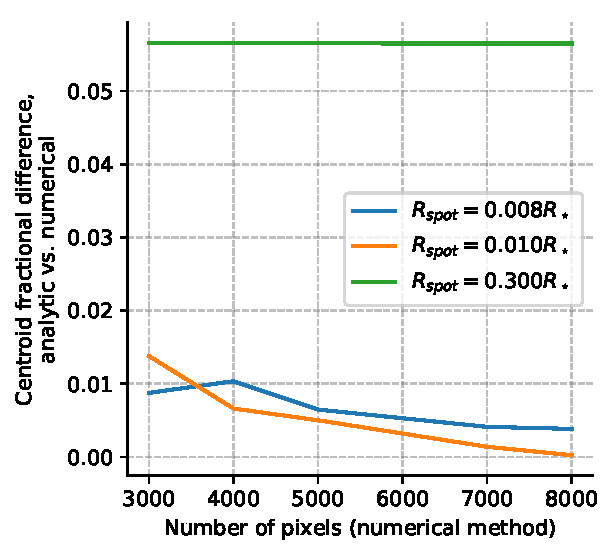
\includegraphics[scale=0.75]{gaia/validation.pdf}
\caption{We validate the two centroid approximations against one another, finding that the stellar centroids agree to better than $6\%$ for all spots considered in this work.}
\label{fig:valid}
\end{figure}

\subsection{Starspot Contrasts} \label{sec:contrast}

Since spot flux contrasts vary as a function of spectral type and filter transmittance, we find a relationship between stellar effective temperature and spot contrasts in temperature and flux. In Figure~\ref{fig:contrast}, we show the observed starspot temperature contrasts of 47 stars reported by \citet{Berdyugina2005}, and we fit a quadratic to the spot temperature contrasts as a function of the stellar photosphere effective temperature. We estimate the spot contrast in the Gaia $G$-band by integrating blackbody radiance curves with the temperatures of the photosphere and spot convolved, with the $G$ filter transmittance.

The Sun's spot contrast in the $G$ band, weighting by the relative areas in the penumbrae and umbrae, is $c\sim0.7$. The best-fit quadratic is consistent with $c = 0.7 \pm 0.1$ for stars with spectral types M2 to G2. Given that 73\% of the stars considered in this paper are within that range of spectral types, we choose to use spot contrast $c=0.7$ for all stars (more on the star sample in Section~\ref{sec:jitter}).

\begin{figure}
\centering
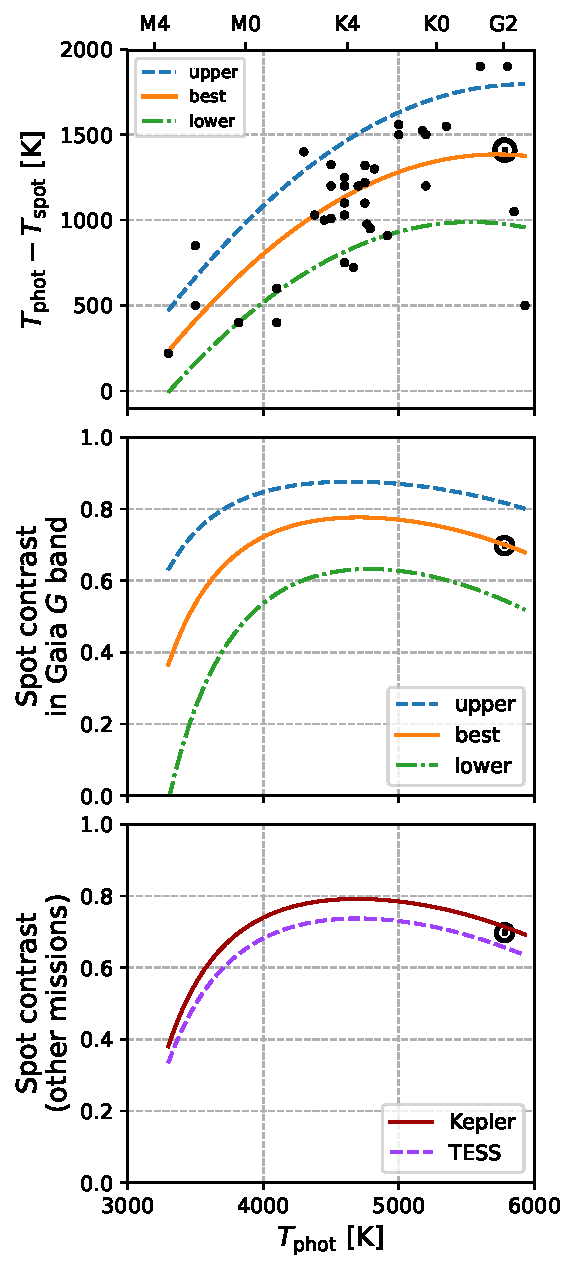
\includegraphics[scale=0.85]{gaia/contrasts.pdf}
\caption{{\sl Upper}: Measured temperature difference between the the mean stellar photosphere temperature $T_{\mathrm{phot}}$ and the starspot temperature $T_{\mathrm{spot}}$, as a function of $T_{\mathrm{phot}}$ (black circles), compiled by \citet{Berdyugina2005}. The middle curve labeled ``best'' is a quadratic fit to the spot contrasts. The  ``min,'' and ``max'' curves roughly approximate the lower and upper envelopes of the spot contrast observations. The Sun's contrast is marked with the symbol $\odot$. 
{\sl Middle}: Spot flux contrasts, approximated by integrating blackbody radiance curves with the temperatures of the photosphere and spot, convolved with the Gaia $G$ bandpass. The area-weighted mean sunspot contrast is $c=0.7$, marked with $\odot$. Stars from spectral types M2 to G2 are consistent with $c=0.7\pm0.1$, so we adopt $c=0.7$ for all stars considered in Section~\ref{sec:jitter}.
{\sl Lower}: Starspot flux contrasts, this time integrated over the Kepler (red curve) and TESS (purple dashed curve) bandpasses. Here we show only the contrast curves for the best-fit quadratic spot temperature relation labeled ``best'' in the uppermost panel. Spot contrasts observed with both the \kepler and TESS missions are within 5\% of the Gaia mission spot contrast.
\label{fig:contrast}}
\end{figure}

\section{Simulating starspot-induced astrometric jitter} \label{sec:sim}

We compute stellar centroid jitter for the starspot distributions of the Sun, GJ 1243 and KIC 7174505. These stars represent different examples of magnetic activity --- the Sun has many small, short-lived spots; GJ 1243 has a few large, long-lived spots; and KIC 7174505 may have extremely large spots. The differences in activity may arise from different dynamo mechanisms for each star, since the Sun has a convective envelope, and GJ 1243 may be fully convective. The configuration of spots on KIC 7174505 and GJ 1243 can be significantly more asymmetric than sunspots, thus producing much larger astrometric signals. In general, the stellar inclination angles for a stars is not known, so we assume that best-case scenario the stars all have stellar inclination $i_s = 90^\circ$, with their rotation axes aligned with the sky plane.

A third star with a well-characterized spot distribution the K4V star HAT-P-11. We do not consider HAT-P-11 because its spectral type and activity is an intermediate case between the Sun and GJ 1243. It has a Sun-like distribution of spots, and spot coverage between that of the Sun and GJ 1243 \citep{Morris2017a, Morris2017b, Davenport2015}. 

\subsection{The Sun} \label{sec:sun}

The Sun will always be the star with the longest-running record of starspot positions and sizes, so we begin by estimating the sunspot-induced astrometric jitter for a distant observer. 

We collect sunspot positions and areas from the Mount Wilson Observatory (MWO) sunspot catalog of \citet{Howard1984}, which spans seven activity cycles from 1917--1985. The sunspot umbral areas are reported in units of solar hemispheres $A_{\mathrm{umb}}$, which are related to the total spot radii $R_{\mathrm{spot}}$ in units of solar radii $R_\odot$ by
\begin{equation}
\frac{R_{\mathrm{spot}}}{R_\odot} = \sqrt{2 (A_{\mathrm{umb}} + A_{\mathrm{pen}})},
\end{equation}
where $A_{\mathrm{pen}}$ is the area in penumbrae. Following \citet{Solanki2003}, we adopt the the penumbral-to-umbral area ratio to be approximately $A_{\mathrm{pen}}/A_{\mathrm{umb}} \sim 4$, so $A_{\mathrm{umb}} + A_{\mathrm{pen}} = 5 A_{\mathrm{umb}}$, and 
\begin{equation}
R_{\mathrm{spot}} \approx \sqrt{10 A_{\mathrm{umb}}} R_\odot.
\end{equation}
Also following \citet{Solanki2003}, we chose the mean flux emitted by a sunspot to be 70\% of the flux of the mean photosphere. 

We define the centroid of the Sun as the flux-weighted mean astrometric position of the Sun in the sky plane for an observer with perfect seeing. We compute the solar centroid by integrating over the Earth-facing solar surface, using all spots reported by \citet{Howard1984}. 

\begin{figure}
\begin{center}
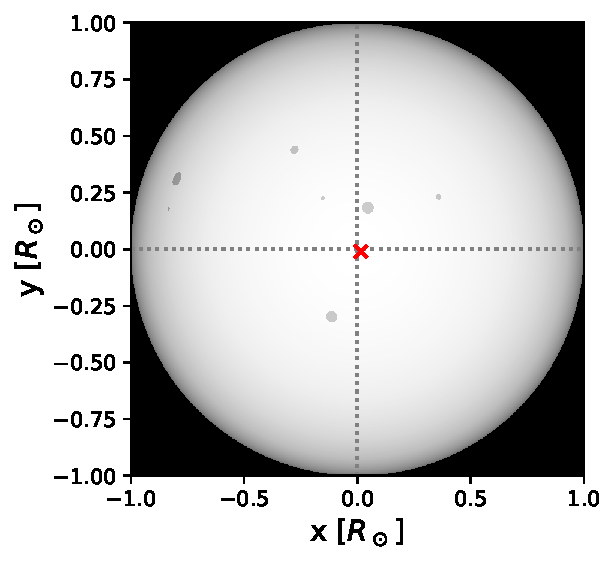
\includegraphics[scale=0.8]{gaia/example_sun.pdf}
\end{center}
\caption{Example sunspot record of the Sun on 1959 May 10 UTC. The gray circles represent sunspots, the white disk represents the solar photosphere. The red ``x'' represents the solar centroid in this image, exaggerated by a factor of 100 to make its offset from the origin visible on the diagram.} \label{fig:sunexample}
\end{figure}
A typical entry in the MWO catalog records about three spots in a day, reaching up to 14 spots on the most active day recorded. The median sunspot radius is $R_{\mathrm{spot}} \approx 0.01 R_\odot$. Recorded spot longitudes span the range $[-60^\circ, 51]$ and latitudes span $[-44^\circ, 51^\circ]$. We plot an example sunspot record from 1959 May 10 UTC in Figure~\ref{fig:sunexample}.

The simple sunspot model does not account for faculae, which are bright components of active regions on the Sun. We ignore faculae in our models of the rotationally modulated stellar centroid calculations for two reasons. First, sunspots dominate the Sun's variability in the optical (though the total solar irradiance integrated over all wavelengths is actually greater at active maximum than minimum) \citep{Shapiro2016}. In addition, the impact of faculae on solar brightness modulations would be greatest for an observer viewing the Sun pole-on \citep{Radick1998, Shapiro2016}, but we consider equator-on configurations in this work. 

\begin{figure}
\begin{center}
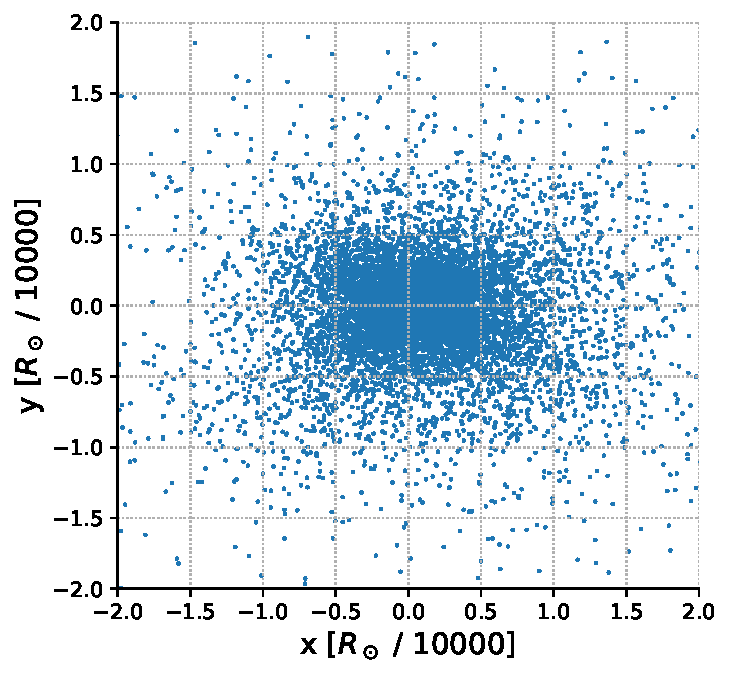
\includegraphics[scale=0.6]{gaia/photocenter_motion.pdf}
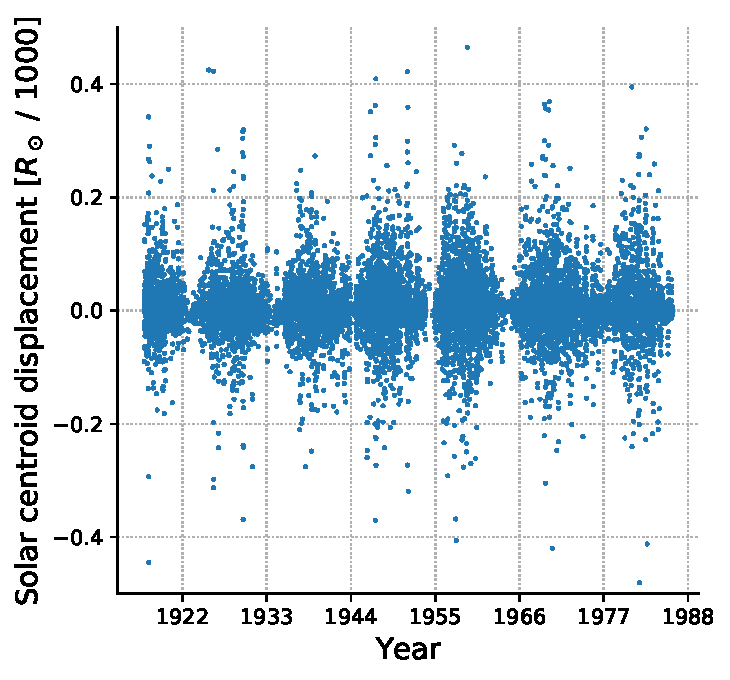
\includegraphics[scale=0.6]{gaia/solar_centroid_displacement.pdf}
\end{center}
\caption{\textsl{Upper}: Position of the solar centroid from 1917--1985, accounting only for astrometric shift due to sunspots. The $y$ coordinate is aligned with the solar rotation axis, and the spread in centroids is broader about the equatorial coordinate. \textsl{Lower}: The absolute centroid displacement from the true solar centroid, $r=\sqrt{x^2+y^2}$, throughout seven activity cycles. Near activity maximum, the centroid displacement is greater than at minimum.} \label{fig:centroid}
\end{figure}
The distribution of centroids of the Sun at each date in the \citet{Howard1984} catalog is shown in Figure~\ref{fig:centroid}. The median absolute deviation of the centroids in the $x$ and $y$ directions are 24 and $15 \mu R_\odot$, respectively. 

For comparison, the reflex motion of the Sun about the barycenter due to Jupiter's orbit is roughly the size of the solar radius. The Sun's reflex motion due to the Earth is about $600 \mu R_\odot$, which is still larger than the scale of sunspot-induced astrometric jitter. Once Keplerian orbits are removed from the astrometric measurements of planet-hosting stars, the residual scatter may contain the signals stellar activity discussed here.

\subsection{GJ 1243}

The distribution of sunspots on the solar photosphere is dictated by the physics of the solar dynamo \citep[see reviews by][]{Charbonneau2014, Hathaway2015}. Mid- to late-M dwarfs are expected to have fully-convective envelopes, and thus their dynamo activity must be driven by different physical mechanisms than the Sun's \citep{Morin2010}. The distribution of small starspots on fully-convective stars (as a function of age) is not yet known, in general.

One low mass star with a constrained spot distribution is the M4 dwarf GJ 1243. \citet{Davenport2015} fit the \kepler photometry of GJ 1243 with a spot model, and found that the rotational modulation is consistent with two starspots rotating differentially, with lifetimes of order $\sim$years. The authors estimated that the spots could be as large as $R_{\mathrm{spot}} \sim 0.3 R_\star$ --- significantly larger than the largest sunspots relative to the solar radius. The spot latitudes are degenerate with the stellar inclination, so the precise spot latitudes are unknown. The best-fit spot models of \citet{Davenport2015} prefer one spot near the pole, and one spot at lower latitudes. We note that small spots analogous in scale to sunspots may also be present on GJ 1243, but the rotational modulation was dominated by the two largest spots, so we study the astrometric jitter caused by those  dominant spots \citep{Davenport2015}.

We adopt the low-latitude starspot of GJ 1243 as another prototype for producing astrometric jitter. When compared with the relatively small sunspots, the large, low-latitude spot observed on GJ 1243 can drive significantly more centroid jitter. To construct a best-case scenario for observing spot-induced jitter, we place a spot with radius $R_{\mathrm{spot}} = 0.3R_\star$ on the stellar equator, and view it with stellar inclination $i_s = 90^\circ$. 

We compute the centroid of GJ 1243 throughout a full rotation following the procedure in Section~\ref{sec:sun}. The maximum displacement of the centroid of GJ 1243 is $0.01 R_\star$ --- roughly a factor of 10 greater than the maximum observed solar astrometric jitter. 

\subsection{KIC 7174505} \label{sec:superflarestar}

\begin{figure}
\begin{center}
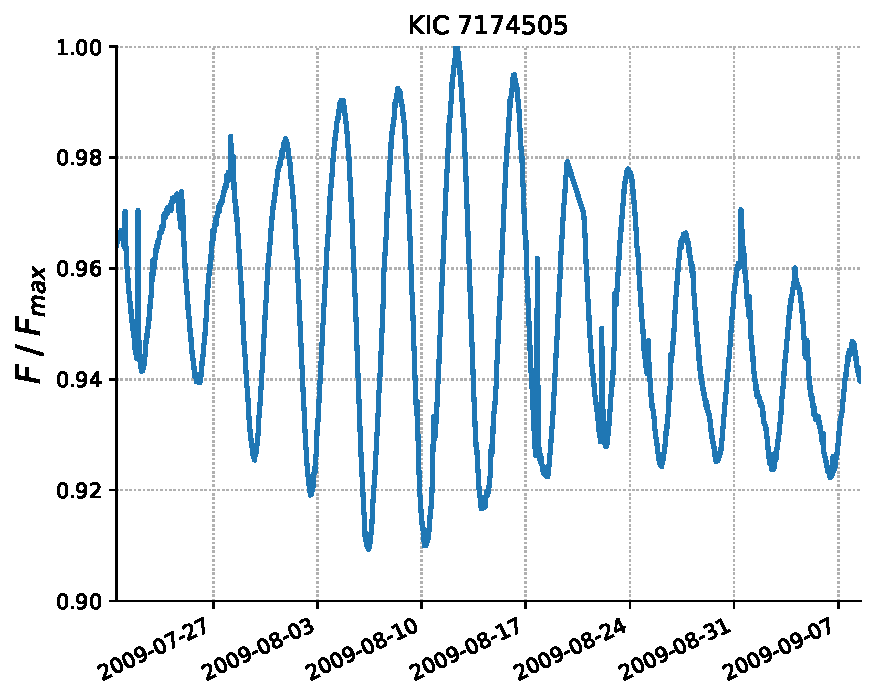
\includegraphics[scale=0.5]{gaia/KIC7174505_lightcurve.pdf}
\end{center}
\caption{A portion of the \kepler light curve of superflare star KIC 7174505, which shows large flux modulation with the rotational period of the star,  $P_{\mathrm{rot}} = 3.832 \pm 0.005$ days \citep{McQuillan2014}.} \label{fig:kic}
\end{figure}

Young G stars in the \kepler field which produce superflares have been the subjects of extensive follow-up observations in the literature \citep[see e.g.:][]{Maehara2012, Maehara2017, Karoff2016, Notsu2013, Notsu2015a, Notsu2015b}. One star with large rotational flux modulation is the superflare star KIC 7174505, with $T_{\mathrm{eff}} \approx 5411$ K and rotation period $P_{\mathrm{rot}} = 3.832 \pm 0.005$ days \citep{Mathur2017, McQuillan2014}. \kepler observed 29 large flare eventson this star, with energies ranging from $7\times10^{34}$ to $2 \times10^{35}$ ergs \citep{Shibayama2013}. A portion of the \kepler light curve of KIC 7174505 is shown in Figure~\ref{fig:kic}.

\citet{Shibayama2013} estimate the spot covering fraction on KIC 7174505 from the rotational modulation of the \kepler light curve. Their estimate of the minimum spotted area is roughly 20\% of the stellar hemisphere, which could be concentrated into one or many spots. If we calculate the radius of a single, circular spot with an area equivalent to 20\% of the stellar hemisphere, we have $R_{\mathrm{spot}}/R_\star = 0.63$. We use this extremely large spot as a limiting case in our calculations for spot-induced astrometric jitter. 

We compute the centroid of KIC 7174505 throughout a full rotation following the procedure in Section~\ref{sec:sun}. The maximum displacement of the centroid of KIC 7174505 is $0.05 R_\star$ --- a factor of five greater than the maximum observed astrometric jitter of GJ 1243. 

\subsection{Expected starspot-induced jitter} \label{sec:jitter}

We calculate the expected starspot-induced jitter for bright, cool, main sequence stars that will be observed by Gaia. To select stars meeting these criteria, we choose stars with Gaia magnitude $G < 7$ from the Tycho-Gaia Astrometric Solution (TGAS) catalog \citep{Michalik2015}. TGAS combines early Gaia astrometry with measurements from the Tycho-2 astrometric mission to solve for parallaxes of millions of nearby stars. We use Tycho photometry in the VT and BT bands, and the combined Tycho-2/Gaia parallaxes to construct a color-magnitude diagram of the bright TGAS stars. We narrow our sample to stars on the main sequence with colors $0.6 < B - V < 2$. These 8,896 stars are highlighted in red on the color-magnitude diagram in Figure~\ref{fig:hr}. It is likely that there are binaries in this sample of stars. We include all stars in our analysis until reporting the best-case targets in Table~\ref{tab:stars}, which have been filtered to remove known binaries.

The TGAS sample does not include the brightest stars in the sky \citep{Michalik2015}. Ongoing efforts throughout the beginning of the Gaia mission have made progress towards measuring astrometry of naked-eye stars, and it is possible that ultimately there will be no bright limit for Gaia astrometry \citep{Martin-Fleitas2014, Sahlmann2016}. Since the final mission bright limit is not yet established, we choose to consider only the stars with Gaia astrometry already published in TGAS, and ignore the brighter stars which may be accessible to Gaia astrometry in the future.  

\begin{figure}
\begin{center}
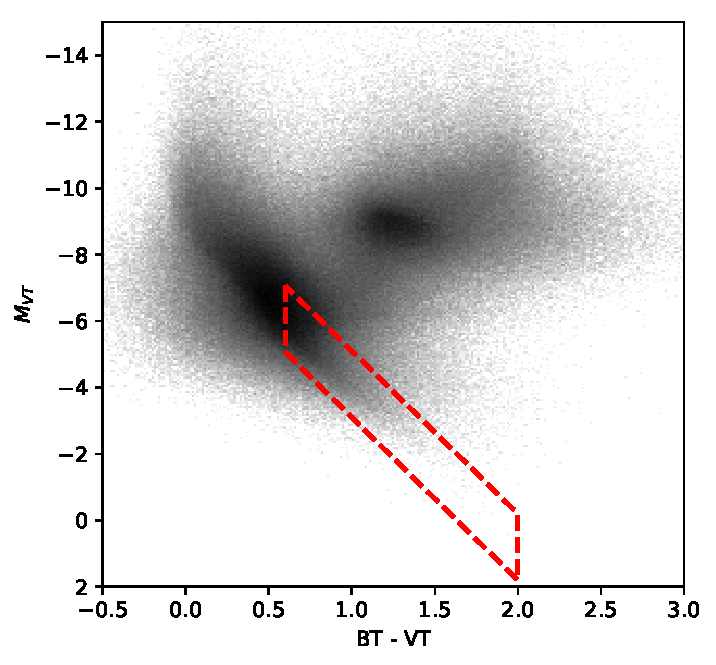
\includegraphics[scale=0.65]{gaia/hr.pdf}
\end{center}
\caption{Color-magnitude diagram for stars brighter than $G < 12$ in the TGAS catalog, where the shading is the logarithm of density of stars in each pixel. $BT$ and $VT$ are the Tycho-2 bandpasses,  similar to Johnson-Cousins $B$ and $V$. We select only stars within the red polygon, which are likely main sequence stars of approximately solar spectral type or later.} \label{fig:hr}
\end{figure}

We calculate Gaia's expected end-of-mission astrometric precision, $\sigma_{\mathrm{Gaia}}$, for the stars in the bright sample. \citet{Perryman2014} outline an algorithm for calculating the expected Gaia astrometric precision for any star, which we reproduce here. The astrometric signal-to-noise achieved in a single Gaia visit $\sigma_{\mathrm{fov}}$ can be computed with:
\begin{equation}
\sigma_{\mathrm{fov}}^2 = \sigma_\eta^2/9 + \sigma_{\mathrm{att}}^2 + \sigma_{\mathrm{cal}}^2
\end{equation}
where the contributions from attitude errors $\sigma_{\mathrm{att}}$ and calibration errors $\sigma_{\mathrm{cal}}$ are both approximately $\sigma_{\mathrm{att}} \approx \sigma_{\mathrm{cal}} = 20 \,\mathrm{\mu arcseconds}$, and the centroiding error $\sigma_\eta$ for each of Gaia's nine CCDs is	
\begin{equation}
\sigma_\eta^2 = 53000 z + 310 z^2.
\end{equation}
$z$ is a function of the inverse number of photons in the image, which is a function of a star's $G$ magnitude,
\begin{equation}
z = 10^{0.4\left(\max[G, 12] - 15\right)}. \label{eqn:z}
\end{equation}
The number of expected visits at a given star over the nominal five-year mission $N^\prime_{\mathrm{fov}}$ is a function of the galactic latitude $b$ of the star (see \citealt{Perryman2014} Table 1 for $N^\prime_{\mathrm{fov}}$ estimates at each $b$). The maximum number of photons received from stars brighter than $G < 12$ is capped by CCD gating, which prevents saturation \citep{Perryman2014}. One consequence of this observing strategy is that the astrometric precision is roughly uniform for all targets brighter than $G < 12$. 

Thus, we can approximate the Gaia end-of-mission astrometric precision for each bright star in the sample with 
\begin{equation}
\sigma_{\mathrm{Gaia}}(G, b) = \sigma_{\mathrm{fov}}(G) / \sqrt{N^\prime_{\mathrm{fov}}(b)}. 
\end{equation}
In other words, the distribution of the Gaia-measured centroids of a single, inactive star without companions will have RMS width $\sigma_{\mathrm{Gaia}}$. Barring unanticipated systematics, scatter measured in the centroid of a star exceeding $\sigma_{\mathrm{Gaia}}$ may be interpreted as the signature of stellar multiplicity, massive planets, or starspots.

\subsection{Sun-like distribution of starspots} \label{sec:sunspot_jitter}

We calculate the spot-induced centroid jitter for the bright TGAS main sequence stars, assuming a Sun-like distribution of spots. We convert the centroid jitter observed on the Sun, in units of $R_\odot$, to the expected RMS angular astrometric jitter $\sigma_{\mathrm{jitter}}$ by observing the solar centroid offsets at the distance of each star in the TGAS sample. Then we normalize the observed jitter by the expected Gaia astrometric uncertainty. 

The expected astrometric jitter produced by a Sun-like distribution of starspots on the stars in the bright TGAS main sequence sample is shown in Figure~\ref{fig:jitter}. The spot-induced jitter $\sigma_{\mathrm{jitter}}$ is normalized by the cumulative, end-of-mission astrometric uncertainty of Gaia, after considering the single-measurement astrometric precision on that star, and the total number of measurements during the nominal five-year mission. Even for the brightest star in the sample, the K0V star $\sigma$ Draconis ($G = 4.71$), the spot-induced jitter is only 1\% of the expected astrometric uncertainty. Measurements of astrometric starspot jitter from Sun-like spot distributions are thus beyond the reach of the nominal five-year Gaia mission.

%\begin{figure}
%\begin{center}
%\includegraphics[scale=0.65]{sunspot_jitter.pdf}
%\end{center}
%\caption{Maximum expected starspot-induced jitter for nearby Gaia stars, assuming a Sun-like spot distribution and stellar inclination $i_s = 90^\circ$, normalized by the estimated end-of-mission astrometric uncertainty.} \label{fig:jitter_sun}
%\end{figure}

\subsection{GJ 1243-like distribution of starspots} \label{sec:gj1243_jitter}

%\begin{figure}
%\begin{center}
%\includegraphics[scale=0.65]{gj1243_jitter.pdf}
%\end{center}
%\caption{Maximum expected starspot-induced jitter for nearby Gaia stars, assuming a starspot distribution like GJ 1243 and stellar inclination $i_s = 90^\circ$, normalized by the estimated end-of-mission astrometric uncertainty.} \label{fig:jitter_gj1243}
%\end{figure}

We calculate the spot-induced centroid jitter for the bright TGAS main sequence stars, assuming a GJ 1243-like distribution of spots. We convert the centroid jitter observed on GJ 1243, in units of $R_\star$, to the expected RMS angular astrometric jitter $\sigma_{\mathrm{jitter}}$ by observing the stellar centroid offsets at the distance of each star in the TGAS sample. We estimate stellar radii for each star using the color--radius relations of \citet{boyajian2012}, and for a small subset of the stars, we combine the interferometric stellar angular diameters from \citet{boyajian2012} with TGAS parallaxes \citep{Michalik2015}. Then we normalize the observed jitter by the expected Gaia astrometric uncertainty. 

The expected astrometric jitter produced by a GJ 1243-like distribution of starspots on the stars in the bright TGAS main sequence sample is shown in Figure~\ref{fig:jitter}. The starspot jitter is comparable or less than the predicted astrometric uncertainty for all stars considered here. At the end of the nominal five-year mission, Gaia astrometry could not detect GJ 1243-like activity on these stars.

\subsection{KIC 7174505-like distribution of starspots} \label{sec:kic_jitter}

%\begin{figure}
%\begin{center}
%\includegraphics[scale=0.65]{KIC7174505_jitter.pdf}
%\end{center}
%\caption{Maximum expected starspot-induced jitter for nearby Gaia stars, assuming a starspot distribution like KIC 7174505 and stellar inclination $i_s = 90^\circ$, normalized by the estimated end-of-mission astrometric uncertainty.} \label{fig:jitter_kic}
%\end{figure}

We calculate the spot-induced centroid jitter for the bright TGAS main sequence stars with a distribution of starspots like KIC 7174505 following the procedure outlined in Section~\ref{sec:gj1243_jitter}. The expected astrometric jitter is shown in Figure~\ref{fig:jitter}. The starspot jitter is larger than the predicted astrometric uncertainty by a factor of three for six stars in the sample, and the jitter exceeds the noise by a factor of six for one non-binary star: AX Mic. We discuss these stars in more detail in Section~\ref{sec:targets}. Gaia astrometry can detect the most extreme centroid offsets even in a fraction of the nominal five-year mission.

\begin{figure}
\begin{center}
\includegraphics[scale=0.6]{gaia/summary.pdf}
\end{center}
\caption{Maximum expected starspot-induced jitter for 8,896 nearby Gaia stars in TGAS, normalized by the estimated astrometric uncertainty for a nominal 5 year mission, assuming starspot distributions like the Sun, GJ 1243, and KIC 7174505. These maximum jitter estimates only consider stellar inclination $i_s = 90^\circ$. Details for the eight best non-binary stars are enumerated in Table~\ref{tab:stars}.} \label{fig:jitter}
\end{figure}

\subsection{Comparison with other works}

\citet{Eriksson2007} and \citet{Catanzarite2008} devise starspot jitter models based on observations of the Sun and other stars. Both groups report a maximum centroid jitter of about $\sim 2 \,\mu$AU for solar-like activity, which is a bit smaller than our maximum estimate of the solar centroid offset based on the observations of \citet{Howard1984} of $\sim 3 \,\mu$AU. \citet{Eriksson2007} also estimate the centroid offsets for M2--M9V type stars in the range $0.4-10 \,\mu$AU, which is smaller than our expectation for the jitter from a GJ1243-like spot distribution, which contributes $\sigma_{\mathrm{jitter}} \approx 35\, \mu$AU. We are unable to find analogous estimates in the literature of starspot jitter from superflare stars like KIC 7174505, which can produce apparent jitter of $100\,\mu$AU.

\subsection{Activity cycles}

The number of sunspots and their latitude distribution changes throughout the solar activity cycle. Near activity minimum, there are sometimes no spots on the Sun at all, and near maximum there can be more than ten. A distant observer could measure centroid offsets due to starspots near activity maximum, but the jitter would diminish at activity minimum -- Figure~\ref{fig:centroid} shows the varying scatter in the solar centroid throughout seven solar activity cycles based on real solar observations. 

We showed in Section \ref{sec:sim} that sunspots would be undetectable by astrometric jitter, jitter from GJ 1243-like spots may be detectable, and jitter from KIC 7174505 would be detected handily for the nearest stars. Is the astrometric signal-to-noise and sampling in time sufficient to measure changes in astrometric jitter throughout stellar activity cycles? 

Here we consider the best-case scenario for detecting activity cycles on stars with spots like KIC 7174505. We seek to determine the difference in astrometric jitter near activity minimum, when $\sigma_{\mathrm{jitter}} \rightarrow 0$, and near activity maximum, when we assume the maximum jitter is achieved by the starspot distribution observed on KIC 7174505. 

Suppose KIC 7174505-like stars have an activity cycle period $P_{\mathrm{cyc}} \sim 10$ years, and spend five years near maximum and five years near minimum. If the Gaia extended mission observed that star over an extended mission lasting 10 years, it will measure the stellar centroid $N^\prime_{\mathrm{fov}}$ times near activity minimum, when the astrometric centroid scatter will be entirely contributed by random and systematic errors. We simulate these observations by drawing $N^\prime_{\mathrm{fov}}$ samples from the distribution $\mathcal{N}(0, \sigma_{\mathrm{fov}}^2)$. Then we observe each star another $N^\prime_{\mathrm{fov}}$ times near activity maximum during a five-year extended mission, when the astrometric scatter will be the quadrature sum of the random errors $\sigma_{\mathrm{fov}}$ and the spot-induced jitter $\sigma_{\mathrm{jitter}}$. We simulate these observations by drawing $N^\prime_{\mathrm{fov}}$ samples from the distribution $\mathcal{N}(0, \sigma_{\mathrm{fov}}^2 + \sigma_{\mathrm{jitter}}^2)$. We compute the confidence of the cycle detection measurement with the two-sample Anderson-Darling and Komolgorov-Smirnov (KS) tests to measure the difference in centroid distributions observed at activity maximum and minimum.

In Table~\ref{tab:stars} we list the statistical significance of the difference between the distribution of centroids near active maximum and minimum, for the bright TGAS sample in an extended 10 year Gaia mission. The stars considered show insignificant detections of an activity cycle in this highly-optimized scenario for detecting activity cycles through Gaia astrometry, where we assumed a highly asymmetric spot distribution and an ideal stellar inclination of $i_s = 90^\circ$. We comment on the properties of the star with the best detection of any activity, AX Mic, in the next section.

The activity cycle detection confidences in Table~\ref{tab:stars} assume that we can unambiguously split the astrometric measurements into maximum and minimum activity subsets. In practice, we will not know the phase of each star's activity cycle \textit{a priori}. However, Gaia radial velocity spectra of the calcium infrared triplet may allow us to independently identify phases in activity cycles. The calcium infrared triplet is a calibrated indicator of chromospheric activity \citep[see e.g.:][]{Chmielewski2000, Cenarro2001, Cauzzi2008, Zerjal2013, BoroSaikia2016, Robertson2016, Martin2017}. True cycles in astrometric jitter should be accompanied by increased emission in the infrared triplet \citep{Andretta2005, Busa2007}. A possible third independent measurement of activity cycles from Gaia is the time-series photometry it will collect, which may yield long-baseline photometry similar to the \kepler full-frame images, which \citet{Montet2017} used to search for activity cycles in \kepler stars.

\subsection{Sensitivity to spot coverage}

It is common to use stellar variability as an estimate of the spot coverage
of stars;  this is adequate for stars that are affected by a single spot,
or two anti-podal spots since only one spot is present on the visible disk
at a time.  Unfortunately, more than two spots that are distributed 
in longitude
cause a weaker amplitude variability:  as one spot rotates off of the
visible disk of the star, another rotates onto it, causing a reduction in
the overall amplitude of variability.  A similar effect has been pointed
out in the context of planetary mapping:  the odd spherical harmonics
induce no change in brightness \citep{Cowan2008}.

In particular, a distribution of three spots with 120$^\circ$ separation
can lead to a very small amplitude of variability.  However, the
astrometric signal of three spots can still be strong despite weak
flux variability. Figure~\ref{fig:photo_vs_astro} shows the relative 
amplitude of variability of the total flux for one, two and three equatorial
spots, distributed evenly in longitude, and viewed at $i_s = 90^\circ$.  In the one- and two- spot cases, the relative
amplitude of variability is similar for photometry and astrometry.
However, in the three-spot case, the photometric variability is
suppressed by a factor of 6.5 relative to the astrometric variability.

\begin{figure}
    \centering
    \includegraphics[scale=0.38]{gaia/n_spots.pdf}
    \caption{Relative amplitude of variability for one (left),
    two (middle) and three (right) spots of equal radii, in flux (blue)
    and astrometric angle (orange dashed).}
    \label{fig:photo_vs_astro}
\end{figure}

\section{Best targets for activity detection with Gaia} \label{sec:targets}

We evaluate the astrometric signal-to-noise expected from the nominal five year Gaia mission for the brightest, nearest main sequence stars in the TGAS sample, and list the results for the eight best candidates in Table~\ref{tab:stars}. The last column of the table denotes the expected scale of starspot jitter normalized by Gaia's astrometric precision $\sigma_{\mathrm{jitter}}/\sigma_{\mathrm{Gaia}}$, in the extreme case of a KIC 7174505-like starspot configuration, observed with stellar inclination $i_s = 90^\circ$. This should be treated as an upper-limit on the astrometric signal that starspots could produce on main sequence stars. In the sections that follow, we examine measurements of each star's activity in the literature.

\begin{table*}
\begin{tabular}{lccccccccccc}
Star & HIP & Spectral & $R_\star$ & $G$ & Distance & $N^\prime_{\mathrm{fov}}$ & $\sigma_{\mathrm{jitter}}$ & $\sigma_{\mathrm{jitter}}/\sigma_{\mathrm{Gaia}}$ & \multicolumn{2}{c}{Best-case cycle sig.:} \\ 
 &  & Type & [$R_\odot$] & [mag] & [$\mathrm{pc}$] & & [$\mathrm{\mu as}$] & (S/N) & KS & Anderson\\ \hline\hline
AX Mic & 105090 & M1V & 0.589\tablenotemark{a} & 5.881 & 3.98 & 107.4 & 20.0 & 6.1 & 0.45 & 0.37 \\
$\sigma$ Dra & 96100 & K0V & 0.789\tablenotemark{a} & 4.711 & 5.76 & 58.5 & 18.5 & 4.1 & 0.5 & 0.43 \\
GX And & 1475 & M2V & 0.459\tablenotemark{b} & 7.096 & 3.56 & 55.6 & 17.4 & 3.8 & 0.48 & 0.43 \\
HD 79211 & 120005 & M0V & 0.572\tablenotemark{b} & 6.948 & 6.29 & 107.4 & 12.3 & 3.7 & 0.51 & 0.45 \\
LHS 3531 & 99701 & M0V & 0.564\tablenotemark{a} & 7.134 & 6.16 & 69.1 & 12.4 & 3.0 & 0.51 & 0.45 \\
HD 222237 & 116745 & K3+V & 0.772\tablenotemark{a} & 6.669 & 11.39 & 107.4 & 9.2 & 2.8 & 0.51 & 0.47 \\
HD 36395 & 25878 & M1.5Ve & 0.531\tablenotemark{b} & 6.986 & 5.65 & 55.6 & 12.7 & 2.8 & 0.53 & 0.48 \\
Gl 625 & 80459 & M1.5V & 0.431\tablenotemark{a} & 8.995 & 6.49 & 107.4 & 9.0 & 2.7 & 0.5 & 0.46 \\
\end{tabular}
\caption{Expected signal-to-noise for the astrometric jitter due to KIC 7174505-like starspots for the best non-binary targets. The columns are: the Hipparcos number, spectral type, Gaia $G$ band magnitude, distance computed from the TGAS parallax, anticipated number of Gaia visits to that particular star $N^\prime_{\mathrm{fov}}$, astrometric jitter from KIC 7174505-like starspots $\sigma_{\mathrm{jitter}}$,  the ratio of the starspot-induced astrometric jitter to the expected astrometric precision over five years of Gaia observations $\sigma_{\mathrm{jitter}}/\sigma_{\mathrm{Gaia}}$. The astrometric precision the targets above (and for Gaia targets brighter than $G < 12$) is constant, $\sigma_{\mathrm{fov}} = 34.2 \,\mu$arcseconds. The last two columns list the expected statistical significance of the astrometric detection of stellar activity cycles for each star over a 10 year extended mission. Radii marked \tablenotemark{a} are estimates from color--radius relation of \citet{boyajian2012}; radii marked \tablenotemark{b} are computed from interferometry by \citet{boyajian2012}, combined with parallaxes from TGAS \citep{Michalik2015}.
\label{tab:stars}}
\end{table*}


\subsection{AX Mic (HD 202560, Gl 825)}

AX Microscopii is a single M1V flare star, with a TGAS distance of 3.9 pc \citep{Young1987, Byrne1981}. \citet{Byrne1989} measured the X-ray flux of AX Mic, and found that its transition region emission is similar to the Sun's, despite being significantly smaller than the Sun. The authors suggest that AX Mic's strong X-ray emission per unit surface area could be achieved with a few active regions on the stellar surface with a filling factor of 0.02\% --- similar to the typical solar spot filling factor.  \citet{Isaacson2010} measured small variations in the chromospheric emission of AX Mic within the range $1.223 < S < 1.386$ with Keck/HIRES.

\subsection{$\sigma$ Draconis (HD 185144)}

$\sigma$ Draconis is a K0V star which was extensively monitored by the Lick-Carnegie Exoplanet Survey Team (LCES) HIRES/Keck Precision Radial Velocity Exoplanet Survey \citep{Butler2017}. The 784 spectra of $\sigma$ Dra reveal an apparent magnetic activity cycle with period $P_{\mathrm{cyc}} \approx 6$ years. 

\subsection{GX And (HD 1326, Gl 15 A)}

GX Andromedae is a M2V flare star at a TGAS distance of 3.6 pc, which hosts at least one exoplanet, usually referred to as Gl 15 A b. The mean chromospheric emission from GX And is $\left< S \right> = 0.524$, and $S$ varies on two timescales. The shorter timescale is likely the stellar rotation period at $P_{\mathrm{rot}} = 44$ d, and the authors suggest that the longer periodicity is a magnetic activity cycle, with period $P_{\mathrm{cyc}} = 9 \pm 2.5$ yr. 

\subsection{HD 79211 (Gl 338 B)}

HD 79211 is a M0Ve flare star. \citet{Pace2013} report significantly variable chromospheric emission on the range $1.55 < S < 2.02$, which is in good agreement with the range observed by \citet{Isaacson2010}, from $1.556 < S < 1.961$. If the variations in chromospheric emission are driven by rotational modulation from active regions, there may be spot-induced jitter to observe in the Gaia astrometry. 

\subsection{HD 36395 (Gl 205)}

HD 36395 is a weakly active M1V star. \citet{Hebrard2016} collected Zeeman-Doppler imaging of HD 36395, and measured the rotation period $P_{\mathrm{rot}} = 33.63 \pm 0.37$ d. The authors found that the star's large-scale magnetic field is mostly poloidal, and the radial velocity periodogram showed signal at multiple periods, separated by about 10 d. They suggest that the multiple periods could arise from dark spots rotating differentially -- one near the pole and one nearer to the equator, in a configuration reminiscent of GJ 1243. 

\subsection{Gl 625 (G 202-48)}

Gl 625 is an M2V star with one known planet --- a super-Earth which orbits at the inner edge of the stellar habitable zone \citep{Mascareno2017}. There are several signals in the periodogram of the $S$-index of Gl 625, which may be the signature of an activity cycle with period $P_{\mathrm{cyc}} = 3.4$ yr. 

\begin{figure}
\centering
\includegraphics[scale=0.6]{gaia/best_targets.pdf}
\caption{The ratio of the starspot-induced astrometric jitter to the expected astrometric precision over five years of Gaia observations $\sigma_{\mathrm{jitter}}/\sigma_{\mathrm{Gaia}}$ for the targets in Table~\ref{tab:stars}. \label{fig:best}}
\end{figure}

\section{Conclusion and Discussion}

The ESA Gaia mission will measure astrometry of bright nearby stars with unprecedented precision. We show that Gaia's astrometric precision will be sufficient to measure the astrometric shifts in the centroids of stars due to dark starspots on some of the nearest low-mass stars, which were included in the TGAS sample. The best candidate for the detection of astrometric jitter induced by starspots is AX Mic, an active M1V flare star. In the most optimistic scenario --- where each star hosts large KIC 7174505-like spots which vary on a 10 year activity cycle --- the variation in astrometric jitter throughout the stellar activity cycles is not detectable with Gaia astrometry alone. The top three targets for astrometric detections of activity (included in the TGAS sample) are: AX Mic, $\sigma$ Dra, and GX And. Upcoming efforts to measure astrometry of the brightest stars with Gaia may expand the sample of stars with detectable activity cycles \citep{Martin-Fleitas2014, Sahlmann2016}.

Other possible applications of astrometric spot variability detection
may include: 1). estimating the total spot coverage since astrometry
is relatively more sensitive to longitudinally-distributed spots compared
total flux (which can affect transit transmission spectra for stars
that host planets); 2). deriving the sky-projected angle of inclination
of stars, which may help to constrain alignment of spin axes of stars; 
3). constraining the 3-D inclination of stars; 4). constraining the North-South asymmetry of spot distributions.  We leave
these ideas for future investigation.

% \facility{ESA/Gaia}

% \section*{Acknowledgements}

% The manuscript benefited from helpful discussions with Andrew Vanderburg. We gratefully acknowledge the software that made this work possible, including: \texttt{ipython} \citep{ipython}, \texttt{numpy} \citep{VanDerWalt2011}, \texttt{scipy} \citep{scipy},  \texttt{matplotlib} \citep{matplotlib}, \texttt{astropy} \citep{Astropy2013}. 

% This work has made use of data from the European Space Agency (ESA)
% mission {\it Gaia} (\url{https://www.cosmos.esa.int/gaia}), processed by
% the {\it Gaia} Data Processing and Analysis Consortium (DPAC,
% \url{https://www.cosmos.esa.int/web/gaia/dpac/consortium}). Funding
% for the DPAC has been provided by national institutions, in particular
% the institutions participating in the {\it Gaia} Multilateral Agreement. 

% This research has made use of the SVO Filter Profile Service (\url{http://svo2.cab.inta-csic.es/theory/fps/}) supported from the Spanish MINECO through grant AyA2014-55216 \citep{rodrigo2012}.

% This research has made use of NASA's Astrophysics Data System. This research has made use of the SIMBAD database, operated at CDS, Strasbourg, France \citep{Wenger2000}. This research has made use of the VizieR catalogue access tool, CDS, Strasbourg, France \citep{Ochsenbein2000}. This research made use of the cross-match service provided by CDS, Strasbourg.

% \bibliographystyle{mnras}
%\bibliographystyle{apj}

% \begin{thebibliography}{}
% \makeatletter
% \relax
% \def\mn@urlcharsother{\let\do\@makeother \do\$\do\&\do\#\do\^\do\_\do\%\do\~}
% \def\mn@doi{\begingroup\mn@urlcharsother \@ifnextchar [ {\mn@doi@}
%   {\mn@doi@[]}}
% \def\mn@doi@[#1]#2{\def\@tempa{#1}\ifx\@tempa\@empty \href
%   {http://dx.doi.org/#2} {doi:#2}\else \href {http://dx.doi.org/#2} {#1}\fi
%   \endgroup}
% \def\mn@eprint#1#2{\mn@eprint@#1:#2::\@nil}
% \def\mn@eprint@arXiv#1{\href {http://arxiv.org/abs/#1} {{\tt arXiv:#1}}}
% \def\mn@eprint@dblp#1{\href {http://dblp.uni-trier.de/rec/bibtex/#1.xml}
%   {dblp:#1}}
% \def\mn@eprint@#1:#2:#3:#4\@nil{\def\@tempa {#1}\def\@tempb {#2}\def\@tempc
%   {#3}\ifx \@tempc \@empty \let \@tempc \@tempb \let \@tempb \@tempa \fi \ifx
%   \@tempb \@empty \def\@tempb {arXiv}\fi \@ifundefined
%   {mn@eprint@\@tempb}{\@tempb:\@tempc}{\expandafter \expandafter \csname
%   mn@eprint@\@tempb\endcsname \expandafter{\@tempc}}}

% \bibitem[\protect\citeauthoryear{{Andretta}, {Bus{\`a}}, {Gomez}  \&
%   {Terranegra}}{{Andretta} et~al.}{2005}]{Andretta2005}
% {Andretta} V.,  {Bus{\`a}} I.,  {Gomez} M.~T.,   {Terranegra} L.,  2005,
%   \mn@doi [\aap] {10.1051/0004-6361:20041745}, \href
%   {http://adsabs.harvard.edu/abs/2005A%26A...430..669A} {430, 669}

% \bibitem[\protect\citeauthoryear{{Astropy Collaboration} et~al.,}{{Astropy
%   Collaboration} et~al.}{2013}]{Astropy2013}
% {Astropy Collaboration} et~al., 2013, \mn@doi [\aap]
%   {10.1051/0004-6361/201322068}, \href
%   {http://adsabs.harvard.edu/abs/2013A%26A...558A..33A} {558, A33}

% \bibitem[\protect\citeauthoryear{{Berdyugina}}{{Berdyugina}}{2005}]{Berdyugina2005}
% {Berdyugina} S.~V.,  2005, \mn@doi [Living Reviews in Solar Physics]
%   {10.12942/lrsp-2005-8}, \href
%   {http://adsabs.harvard.edu/abs/2005LRSP....2....8B} {2, 8}

% \bibitem[\protect\citeauthoryear{{Boro Saikia} et~al.,}{{Boro Saikia}
%   et~al.}{2016}]{BoroSaikia2016}
% {Boro Saikia} S.,  et~al., 2016, \mn@doi [\aap] {10.1051/0004-6361/201628262},
%   \href {http://adsabs.harvard.edu/abs/2016A%26A...594A..29B} {594, A29}

% \bibitem[\protect\citeauthoryear{{Boyajian} et~al.,}{{Boyajian}
%   et~al.}{2012}]{boyajian2012}
% {Boyajian} T.~S.,  et~al., 2012, \mn@doi [\apj] {10.1088/0004-637X/757/2/112},
%   \href {http://adsabs.harvard.edu/abs/2012ApJ...757..112B} {757, 112}

% \bibitem[\protect\citeauthoryear{{Bus{\`a}}, {Aznar Cuadrado}, {Terranegra},
%   {Andretta}  \& {Gomez}}{{Bus{\`a}} et~al.}{2007}]{Busa2007}
% {Bus{\`a}} I.,  {Aznar Cuadrado} R.,  {Terranegra} L.,  {Andretta} V.,
%   {Gomez} M.~T.,  2007, \mn@doi [\aap] {10.1051/0004-6361:20065588}, \href
%   {http://adsabs.harvard.edu/abs/2007A%26A...466.1089B} {466, 1089}

% \bibitem[\protect\citeauthoryear{{Butler} et~al.,}{{Butler}
%   et~al.}{2017}]{Butler2017}
% {Butler} R.~P.,  et~al., 2017, \mn@doi [\aj] {10.3847/1538-3881/aa66ca}, \href
%   {http://adsabs.harvard.edu/abs/2017AJ....153..208B} {153, 208}

% \bibitem[\protect\citeauthoryear{Byrne}{Byrne}{1981}]{Byrne1981}
% Byrne P.~B.,  1981, \mn@doi [Monthly Notices of the Royal Astronomical Society]
%   {10.1093/mnras/195.2.143}, 195, 143

% \bibitem[\protect\citeauthoryear{{Byrne} \& {Doyle}}{{Byrne} \&
%   {Doyle}}{1989}]{Byrne1989}
% {Byrne} P.~B.,  {Doyle} J.~G.,  1989, \aap, \href
%   {http://adsabs.harvard.edu/abs/1989A%26A...208..159B} {208, 159}

% \bibitem[\protect\citeauthoryear{{Catanzarite}, {Law}  \& {Shao}}{{Catanzarite}
%   et~al.}{2008}]{Catanzarite2008}
% {Catanzarite} J.,  {Law} N.,   {Shao} M.,  2008, in Optical and Infrared
%   Interferometry. p. 70132K (\mn@eprint {arXiv} {0807.1930}),
%   \mn@doi{10.1117/12.787904}

% \bibitem[\protect\citeauthoryear{{Cauzzi} et~al.,}{{Cauzzi}
%   et~al.}{2008}]{Cauzzi2008}
% {Cauzzi} G.,  et~al., 2008, \mn@doi [\aap] {10.1051/0004-6361:20078642}, \href
%   {http://adsabs.harvard.edu/abs/2008A%26A...480..515C} {480, 515}

% \bibitem[\protect\citeauthoryear{{Cenarro}, {Cardiel}, {Gorgas}, {Peletier},
%   {Vazdekis}  \& {Prada}}{{Cenarro} et~al.}{2001}]{Cenarro2001}
% {Cenarro} A.~J.,  {Cardiel} N.,  {Gorgas} J.,  {Peletier} R.~F.,  {Vazdekis}
%   A.,   {Prada} F.,  2001, \mn@doi [\mnras] {10.1046/j.1365-8711.2001.04688.x},
%   \href {http://adsabs.harvard.edu/abs/2001MNRAS.326..959C} {326, 959}

% \bibitem[\protect\citeauthoryear{{Charbonneau}}{{Charbonneau}}{2014}]{Charbonneau2014}
% {Charbonneau} P.,  2014, \mn@doi [\araa] {10.1146/annurev-astro-081913-040012},
%   \href {http://adsabs.harvard.edu/abs/2014ARA%26A..52..251C} {52, 251}

% \bibitem[\protect\citeauthoryear{{Chiavassa} et~al.,}{{Chiavassa}
%   et~al.}{2011}]{Chiavassa2011}
% {Chiavassa} A.,  et~al., 2011, \mn@doi [\aap] {10.1051/0004-6361/201015768},
%   \href {http://adsabs.harvard.edu/abs/2011A%26A...528A.120C} {528, A120}

% \bibitem[\protect\citeauthoryear{{Chmielewski}}{{Chmielewski}}{2000}]{Chmielewski2000}
% {Chmielewski} Y.,  2000, \aap, \href
%   {http://adsabs.harvard.edu/abs/2000A%26A...353..666C} {353, 666}

% \bibitem[\protect\citeauthoryear{{Cowan} \& {Agol}}{{Cowan} \&
%   {Agol}}{2008}]{Cowan2008}
% {Cowan} N.~B.,  {Agol} E.,  2008, \mn@doi [\apjl] {10.1086/588553}, \href
%   {http://adsabs.harvard.edu/abs/2008ApJ...678L.129C} {678, L129}

% \bibitem[\protect\citeauthoryear{{Davenport}, {Hebb}  \& {Hawley}}{{Davenport}
%   et~al.}{2015}]{Davenport2015}
% {Davenport} J.~R.~A.,  {Hebb} L.,   {Hawley} S.~L.,  2015, \mn@doi [\apj]
%   {10.1088/0004-637X/806/2/212}, \href
%   {http://adsabs.harvard.edu/abs/2015ApJ...806..212D} {806, 212}

% \bibitem[\protect\citeauthoryear{{Eriksson} \& {Lindegren}}{{Eriksson} \&
%   {Lindegren}}{2007}]{Eriksson2007}
% {Eriksson} U.,  {Lindegren} L.,  2007, \mn@doi [\aap]
%   {10.1051/0004-6361:20078031}, \href
%   {http://adsabs.harvard.edu/abs/2007A%26A...476.1389E} {476, 1389}

% \bibitem[\protect\citeauthoryear{{Gaia Collaboration} et~al.,}{{Gaia
%   Collaboration} et~al.}{2016}]{Gaia2016b}
% {Gaia Collaboration} et~al., 2016, \mn@doi [\aap]
%   {10.1051/0004-6361/201629272}, \href
%   {http://adsabs.harvard.edu/abs/2016A%26A...595A...1G} {595, A1}

% \bibitem[\protect\citeauthoryear{{Gomes da Silva}, {Santos}, {Bonfils},
%   {Delfosse}, {Forveille}, {Udry}, {Dumusque}  \& {Lovis}}{{Gomes da Silva}
%   et~al.}{2012}]{GomesdaSilva2012}
% {Gomes da Silva} J.,  {Santos} N.~C.,  {Bonfils} X.,  {Delfosse} X.,
%   {Forveille} T.,  {Udry} S.,  {Dumusque} X.,   {Lovis} C.,  2012, \mn@doi
%   [\aap] {10.1051/0004-6361/201118598}, \href
%   {http://adsabs.harvard.edu/abs/2012A%26A...541A...9G} {541, A9}

% \bibitem[\protect\citeauthoryear{{Hathaway}}{{Hathaway}}{2015}]{Hathaway2015}
% {Hathaway} D.~H.,  2015, \mn@doi [Living Reviews in Solar Physics]
%   {10.1007/lrsp-2015-4}, \href
%   {http://adsabs.harvard.edu/abs/2015LRSP...12....4H} {12}

% \bibitem[\protect\citeauthoryear{{H{\'e}brard}, {Donati}, {Delfosse}, {Morin},
%   {Moutou}  \& {Boisse}}{{H{\'e}brard} et~al.}{2016}]{Hebrard2016}
% {H{\'e}brard} {\'E}.~M.,  {Donati} J.-F.,  {Delfosse} X.,  {Morin} J.,
%   {Moutou} C.,   {Boisse} I.,  2016, \mn@doi [\mnras] {10.1093/mnras/stw1346},
%   \href {http://adsabs.harvard.edu/abs/2016MNRAS.461.1465H} {461, 1465}

% \bibitem[\protect\citeauthoryear{{Howard}, {Gilman}  \& {Gilman}}{{Howard}
%   et~al.}{1984}]{Howard1984}
% {Howard} R.,  {Gilman} P.~I.,   {Gilman} P.~A.,  1984, \mn@doi [\apj]
%   {10.1086/162315}, \href {http://adsabs.harvard.edu/abs/1984ApJ...283..373H}
%   {283, 373}

% \bibitem[\protect\citeauthoryear{{Hunter}}{{Hunter}}{2007}]{matplotlib}
% {Hunter} J.~D.,  2007, \mn@doi [Computing in Science and Engineering]
%   {10.1109/MCSE.2007.55}, \href
%   {http://adsabs.harvard.edu/abs/2007CSE.....9...90H} {9, 90}

% \bibitem[\protect\citeauthoryear{{Isaacson} \& {Fischer}}{{Isaacson} \&
%   {Fischer}}{2010}]{Isaacson2010}
% {Isaacson} H.,  {Fischer} D.,  2010, \mn@doi [\apj]
%   {10.1088/0004-637X/725/1/875}, \href
%   {http://adsabs.harvard.edu/abs/2010ApJ...725..875I} {725, 875}

% \bibitem[\protect\citeauthoryear{Jones, Oliphant, Peterson  et~al.}{Jones
%   et~al.}{2001}]{scipy}
% Jones E.,  Oliphant T.,  Peterson P.,   et~al., 2001, {SciPy}: Open source
%   scientific tools for {Python}, \url {http://www.scipy.org/}

% \bibitem[\protect\citeauthoryear{{Karoff} et~al.,}{{Karoff}
%   et~al.}{2016}]{Karoff2016}
% {Karoff} C.,  et~al., 2016, \mn@doi [Nature Communications]
%   {10.1038/ncomms11058}, \href
%   {http://adsabs.harvard.edu/abs/2016NatCo...711058K} {7, 11058}

% \bibitem[\protect\citeauthoryear{{Lanza}, {De Martino}  \&
%   {Rodon{\`o}}}{{Lanza} et~al.}{2008}]{Lanza2008}
% {Lanza} A.~F.,  {De Martino} C.,   {Rodon{\`o}} M.,  2008, \mn@doi [\na]
%   {10.1016/j.newast.2007.06.009}, \href
%   {http://adsabs.harvard.edu/abs/2008NewA...13...77L} {13, 77}

% \bibitem[\protect\citeauthoryear{{Maehara} et~al.,}{{Maehara}
%   et~al.}{2012}]{Maehara2012}
% {Maehara} H.,  et~al., 2012, \mn@doi [\nat] {10.1038/nature11063}, \href
%   {http://adsabs.harvard.edu/abs/2012Natur.485..478M} {485, 478}

% \bibitem[\protect\citeauthoryear{{Maehara}, {Notsu}, {Notsu}, {Namekata},
%   {Honda}, {Ishii}, {Nogami}  \& {Shibata}}{{Maehara}
%   et~al.}{2017}]{Maehara2017}
% {Maehara} H.,  {Notsu} Y.,  {Notsu} S.,  {Namekata} K.,  {Honda} S.,  {Ishii}
%   T.~T.,  {Nogami} D.,   {Shibata} K.,  2017, \mn@doi [\pasj]
%   {10.1093/pasj/psx013}, \href
%   {http://adsabs.harvard.edu/abs/2017PASJ...69...41M} {69, 41}

% \bibitem[\protect\citeauthoryear{{Martin-Fleitas}, {Sahlmann}, {Mora},
%   {Kohley}, {Massart}, {Le Roy}  \& {Paulet}}{{Martin-Fleitas}
%   et~al.}{2014}]{Martin-Fleitas2014}
% {Martin-Fleitas} J.,  {Sahlmann} A.,  {Mora} R.,  {Kohley} B.,  {Massart}
%   J.~{L'Hermitte} M.,  {Le Roy} P.,   {Paulet} 2014, Enabling Gaia observations
%   of naked-eye stars, \mn@doi{10.1117/12.2056325}, \url
%   {http://dx.doi.org/10.1117/12.2056325}

% \bibitem[\protect\citeauthoryear{{Martin}, {Fuhrmeister}, {Mittag}, {Schmidt},
%   {Hempelmann}, {Gonz{\'a}lez-P{\'e}rez}  \& {Schmitt}}{{Martin}
%   et~al.}{2017}]{Martin2017}
% {Martin} J.,  {Fuhrmeister} B.,  {Mittag} M.,  {Schmidt} T.~O.~B.,
%   {Hempelmann} A.,  {Gonz{\'a}lez-P{\'e}rez} J.~N.,   {Schmitt} J.~H.~M.~M.,
%   2017, \mn@doi [\aap] {10.1051/0004-6361/201630298}, \href
%   {http://adsabs.harvard.edu/abs/2017A%26A...605A.113M} {605, A113}

% \bibitem[\protect\citeauthoryear{{Mathur} et~al.,}{{Mathur}
%   et~al.}{2017}]{Mathur2017}
% {Mathur} S.,  et~al., 2017, \mn@doi [\apjs] {10.3847/1538-4365/229/2/30}, \href
%   {http://cdsads.u-strasbg.fr/abs/2017ApJS..229...30M} {229, 30}

% \bibitem[\protect\citeauthoryear{{McQuillan}, {Mazeh}  \&
%   {Aigrain}}{{McQuillan} et~al.}{2014}]{McQuillan2014}
% {McQuillan} A.,  {Mazeh} T.,   {Aigrain} S.,  2014, \mn@doi [\apjs]
%   {10.1088/0067-0049/211/2/24}, \href
%   {http://cdsads.u-strasbg.fr/abs/2014ApJS..211...24M} {211, 24}

% \bibitem[\protect\citeauthoryear{{Michalik}, {Lindegren}  \&
%   {Hobbs}}{{Michalik} et~al.}{2015}]{Michalik2015}
% {Michalik} D.,  {Lindegren} L.,   {Hobbs} D.,  2015, \mn@doi [\aap]
%   {10.1051/0004-6361/201425310}, \href
%   {http://adsabs.harvard.edu/abs/2015A%26A...574A.115M} {574, A115}

% \bibitem[\protect\citeauthoryear{{Montet}, {Tovar}  \&
%   {Foreman-Mackey}}{{Montet} et~al.}{2017}]{montet2017}
% {Montet} B.~T.,  {Tovar} G.,   {Foreman-Mackey} D.,  2017, preprint, \href
%   {http://adsabs.harvard.edu/abs/2017arXiv170507928M} {} (\mn@eprint {arXiv}
%   {1705.07928})

% \bibitem[\protect\citeauthoryear{{Morin}, {Donati}, {Petit}, {Delfosse},
%   {Forveille}  \& {Jardine}}{{Morin} et~al.}{2010}]{Morin2010}
% {Morin} J.,  {Donati} J.-F.,  {Petit} P.,  {Delfosse} X.,  {Forveille} T.,
%   {Jardine} M.~M.,  2010, \mn@doi [\mnras] {10.1111/j.1365-2966.2010.17101.x},
%   \href {http://adsabs.harvard.edu/abs/2010MNRAS.407.2269M} {407, 2269}

% \bibitem[\protect\citeauthoryear{{Morris}, {Hebb}, {Davenport}, {Rohn}  \&
%   {Hawley}}{{Morris} et~al.}{2017a}]{Morris2017a}
% {Morris} B.~M.,  {Hebb} L.,  {Davenport} J.~R.~A.,  {Rohn} G.,   {Hawley}
%   S.~L.,  2017a, \mn@doi [\apj] {10.3847/1538-4357/aa8555}, \href
%   {http://adsabs.harvard.edu/abs/2017ApJ...846...99M} {846, 99}

% \bibitem[\protect\citeauthoryear{{Morris} et~al.,}{{Morris}
%   et~al.}{2017b}]{Morris2017b}
% {Morris} B.~M.,  et~al., 2017b, \mn@doi [\apj] {10.3847/1538-4357/aa8cca},
%   \href {http://adsabs.harvard.edu/abs/2017ApJ...848...58M} {848, 58}

% \bibitem[\protect\citeauthoryear{{Notsu} et~al.,}{{Notsu}
%   et~al.}{2013}]{Notsu2013}
% {Notsu} Y.,  et~al., 2013, \mn@doi [\apj] {10.1088/0004-637X/771/2/127}, \href
%   {http://adsabs.harvard.edu/abs/2013ApJ...771..127N} {771, 127}

% \bibitem[\protect\citeauthoryear{{Notsu}, {Honda}, {Maehara}, {Notsu},
%   {Shibayama}, {Nogami}  \& {Shibata}}{{Notsu} et~al.}{2015a}]{Notsu2015b}
% {Notsu} Y.,  {Honda} S.,  {Maehara} H.,  {Notsu} S.,  {Shibayama} T.,  {Nogami}
%   D.,   {Shibata} K.,  2015a, \mn@doi [\pasj] {10.1093/pasj/psv001}, \href
%   {http://adsabs.harvard.edu/abs/2015PASJ...67...32N} {67, 32}

% \bibitem[\protect\citeauthoryear{{Notsu}, {Honda}, {Maehara}, {Notsu},
%   {Shibayama}, {Nogami}  \& {Shibata}}{{Notsu} et~al.}{2015b}]{Notsu2015a}
% {Notsu} Y.,  {Honda} S.,  {Maehara} H.,  {Notsu} S.,  {Shibayama} T.,  {Nogami}
%   D.,   {Shibata} K.,  2015b, \mn@doi [\pasj] {10.1093/pasj/psv002}, \href
%   {http://adsabs.harvard.edu/abs/2015PASJ...67...33N} {67, 33}

% \bibitem[\protect\citeauthoryear{{Ochsenbein}, {Bauer}  \&
%   {Marcout}}{{Ochsenbein} et~al.}{2000}]{Ochsenbein2000}
% {Ochsenbein} F.,  {Bauer} P.,   {Marcout} J.,  2000, \mn@doi [\aaps]
%   {10.1051/aas:2000169}, \href
%   {http://adsabs.harvard.edu/abs/2000A%26AS..143...23O} {143, 23}

% \bibitem[\protect\citeauthoryear{{Pace}}{{Pace}}{2013}]{Pace2013}
% {Pace} G.,  2013, \mn@doi [\aap] {10.1051/0004-6361/201220364}, \href
%   {http://cdsads.u-strasbg.fr/abs/2013A%26A...551L...8P} {551, L8}

% \bibitem[\protect\citeauthoryear{Perez \& Granger}{Perez \&
%   Granger}{2007}]{ipython}
% Perez F.,  Granger B.~E.,  2007, \mn@doi [Computing in Science and Engg.]
%   {10.1109/MCSE.2007.53}, 9, 21

% \bibitem[\protect\citeauthoryear{{Perryman}, {Hartman}, {Bakos}  \&
%   {Lindegren}}{{Perryman} et~al.}{2014}]{Perryman2014}
% {Perryman} M.,  {Hartman} J.,  {Bakos} G.~{\'A}.,   {Lindegren} L.,  2014,
%   \mn@doi [\apj] {10.1088/0004-637X/797/1/14}, \href
%   {http://adsabs.harvard.edu/abs/2014ApJ...797...14P} {797, 14}

% \bibitem[\protect\citeauthoryear{{Radick}, {Lockwood}, {Skiff}  \&
%   {Baliunas}}{{Radick} et~al.}{1998}]{Radick1998}
% {Radick} R.~R.,  {Lockwood} G.~W.,  {Skiff} B.~A.,   {Baliunas} S.~L.,  1998,
%   \mn@doi [\apjs] {10.1086/313135}, \href
%   {http://adsabs.harvard.edu/abs/1998ApJS..118..239R} {118, 239}

% \bibitem[\protect\citeauthoryear{{Robertson}, {Endl}, {Cochran}  \&
%   {Dodson-Robinson}}{{Robertson} et~al.}{2013}]{Robertson2013}
% {Robertson} P.,  {Endl} M.,  {Cochran} W.~D.,   {Dodson-Robinson} S.~E.,  2013,
%   \mn@doi [\apj] {10.1088/0004-637X/764/1/3}, \href
%   {http://adsabs.harvard.edu/abs/2013ApJ...764....3R} {764, 3}

% \bibitem[\protect\citeauthoryear{{Robertson}, {Bender}, {Mahadevan}, {Roy}  \&
%   {Ramsey}}{{Robertson} et~al.}{2016}]{Robertson2016}
% {Robertson} P.,  {Bender} C.,  {Mahadevan} S.,  {Roy} A.,   {Ramsey} L.~W.,
%   2016, \mn@doi [\apj] {10.3847/0004-637X/832/2/112}, \href
%   {http://adsabs.harvard.edu/abs/2016ApJ...832..112R} {832, 112}

% \bibitem[\protect\citeauthoryear{{Rodrigo}, {Solano}  \& {Bayo}}{{Rodrigo}
%   et~al.}{2012}]{rodrigo2012}
% {Rodrigo} C.,  {Solano} E.,   {Bayo} A.,  2012, {SVO Filter Profile Service
%   Version 1.0}, IVOA Working Draft 15 October 2012

% \bibitem[\protect\citeauthoryear{{Sahlmann}, {Mart{\'{\i}}n-Fleitas}, {Mora},
%   {Abreu}, {Crowley}  \& {Joliet}}{{Sahlmann} et~al.}{2016}]{Sahlmann2016}
% {Sahlmann} J.,  {Mart{\'{\i}}n-Fleitas} J.,  {Mora} A.,  {Abreu} A.,  {Crowley}
%   C.~M.,   {Joliet} E.,  2016, in Space Telescopes and Instrumentation 2016:
%   Optical, Infrared, and Millimeter Wave. p. 99042E (\mn@eprint {arXiv}
%   {1605.08347}), \mn@doi{10.1117/12.2231240}

% \bibitem[\protect\citeauthoryear{{Shapiro}, {Solanki}, {Krivova}, {Yeo}  \&
%   {Schmutz}}{{Shapiro} et~al.}{2016}]{Shapiro2016}
% {Shapiro} A.~I.,  {Solanki} S.~K.,  {Krivova} N.~A.,  {Yeo} K.~L.,   {Schmutz}
%   W.~K.,  2016, \mn@doi [\aap] {10.1051/0004-6361/201527527}, \href
%   {http://adsabs.harvard.edu/abs/2016A%26A...589A..46S} {589, A46}

% \bibitem[\protect\citeauthoryear{{Shibayama} et~al.,}{{Shibayama}
%   et~al.}{2013}]{Shibayama2013}
% {Shibayama} T.,  et~al., 2013, \mn@doi [\apjs] {10.1088/0067-0049/209/1/5},
%   \href {http://adsabs.harvard.edu/abs/2013ApJS..209....5S} {209, 5}

% \bibitem[\protect\citeauthoryear{{Solanki}}{{Solanki}}{2003}]{Solanki2003}
% {Solanki} S.~K.,  2003, \mn@doi [\aapr] {10.1007/s00159-003-0018-4}, \href
%   {http://adsabs.harvard.edu/abs/2003A%26ARv..11..153S} {11, 153}

% \bibitem[\protect\citeauthoryear{{Su{\'a}rez Mascare{\~n}o}, {Rebolo}  \&
%   {Gonz{\'a}lez Hern{\'a}ndez}}{{Su{\'a}rez Mascare{\~n}o}
%   et~al.}{2016}]{Mascareno2016}
% {Su{\'a}rez Mascare{\~n}o} A.,  {Rebolo} R.,   {Gonz{\'a}lez Hern{\'a}ndez}
%   J.~I.,  2016, \mn@doi [\aap] {10.1051/0004-6361/201628586}, \href
%   {http://adsabs.harvard.edu/abs/2016A%26A...595A..12S} {595, A12}

% \bibitem[\protect\citeauthoryear{{Su{\'a}rez Mascare{\~n}o}
%   et~al.,}{{Su{\'a}rez Mascare{\~n}o} et~al.}{2017}]{Mascareno2017}
% {Su{\'a}rez Mascare{\~n}o} A.,  et~al., 2017, \mn@doi [\aap]
%   {10.1051/0004-6361/201730957}, \href
%   {http://adsabs.harvard.edu/abs/2017A%26A...605A..92S} {605, A92}

% \bibitem[\protect\citeauthoryear{{Van Der Walt}, {Colbert}  \&
%   {Varoquaux}}{{Van Der Walt} et~al.}{2011}]{VanDerWalt2011}
% {Van Der Walt} S.,  {Colbert} S.~C.,   {Varoquaux} G.,  2011, preprint, \href
%   {http://adsabs.harvard.edu/abs/2011arXiv1102.1523V} {} (\mn@eprint {arXiv}
%   {1102.1523})

% \bibitem[\protect\citeauthoryear{{Wenger} et~al.,}{{Wenger}
%   et~al.}{2000}]{Wenger2000}
% {Wenger} M.,  et~al., 2000, \mn@doi [\aaps] {10.1051/aas:2000332}, \href
%   {http://adsabs.harvard.edu/abs/2000A%26AS..143....9W} {143, 9}

% \bibitem[\protect\citeauthoryear{{Young}, {Sadjadi}  \& {Harlan}}{{Young}
%   et~al.}{1987}]{Young1987}
% {Young} A.,  {Sadjadi} S.,   {Harlan} E.,  1987, \mn@doi [\apj]
%   {10.1086/165057}, \href {http://adsabs.harvard.edu/abs/1987ApJ...314..272Y}
%   {314, 272}

% \bibitem[\protect\citeauthoryear{{{\v Z}erjal} et~al.,}{{{\v Z}erjal}
%   et~al.}{2013}]{Zerjal2013}
% {{\v Z}erjal} M.,  et~al., 2013, \mn@doi [\apj] {10.1088/0004-637X/776/2/127},
%   \href {http://adsabs.harvard.edu/abs/2013ApJ...776..127Z} {776, 127}

% \makeatother
% \end{thebibliography}

% % Don't change these lines
% \bsp	% typesetting comment
% \label{lastpage}
% \end{document}

% End of mnras_template.tex

\chapter{Possible Bright Starspots of TRAPPIST-1}

% \documentclass[preprint2]{aastex62}

% \usepackage{natbib}
% %\bibliographystyle{humannat}

% \usepackage{amsmath}
% \usepackage{hyperref}
% \usepackage{listings}
% \usepackage{color}
% \usepackage{float}
% \usepackage{xspace} 

%\newcommand{\kepler}{\textsl{Kepler}\xspace}
\newcommand{\spitzer}{\textsl{Spitzer}\xspace}

% \begin{document}

% \title{Possible Bright Starspots on TRAPPIST-1}

% \author[0000-0003-2528-3409]{Brett M. Morris}
% \affiliation{Astronomy Department, University of Washington, Seattle, WA 98195, USA}

% \author{Eric Agol}
% \altaffiliation{Guggenheim Fellow}
% \affiliation{Astronomy Department and Virtual Planetary Laboratory, University of Washington, Seattle, WA 98195, USA}
% \author{James R. A. Davenport}
% \altaffiliation{DIRAC Fellow}
% \altaffiliation{NSF Astronomy and Astrophysics Postdoctoral Fellow}
% \affiliation{Astronomy Department, University of Washington, Seattle, WA 98195, USA}
% \affiliation{Department of Physics \& Astronomy, Western Washington University, 516 High St., Bellingham, WA 98225, USA}

% \author{Suzanne L. Hawley}
% \affiliation{Astronomy Department, University of Washington, Seattle, WA 98195, USA}

% \email{bmmorris@uw.edu}

% \begin{abstract}
% The M8V star TRAPPIST-1 hosts seven roughly Earth-sized planets and is a promising target for exoplanet characterization.  \kepler/K2 Campaign 12 observations of TRAPPIST-1 in the optical show an apparent rotational modulation with a 3.3 day period, though that rotational signal is not readily detected in the \spitzer light curve at 4.5 $\mu$m. If the rotational modulation is due to starspots, persistent dark spots can be excluded from the lack of photometric variability in the \spitzer light curve. We construct a photometric model for rotational modulation due to photospheric bright spots on TRAPPIST-1 which is consistent with both the \kepler and \spitzer light curves. The maximum-likelihood model with three spots has typical spot sizes of $R_\mathrm{spot}/R_\star \approx 0.004$ at temperature $T_\mathrm{spot} \gtrsim 5300 \pm 200$ K. We also find that large flares are observed more often when the brightest spot is facing the observer, suggesting a correlation between the position of the bright spots and flare events. In addition, these flares may occur preferentially when the spots are increasing in brightness, which suggests that the 3.3 d periodicity may not be a rotational signal, but rather a characteristic timescale of active regions.
% \end{abstract}

% \keywords{star spots, stellar activity}

% \object{TRAPPIST-1}

\section{Introduction}

TRAPPIST-1 is an M8V star and host to at least seven Earth-sized planets \citep{Gillon2016,Gillon2017}. It was observed with \spitzer at the IRAC-2 4.5 $\mu$m band for 20 days \citep{Gillon2017,Delrez2018}, and 76 days later it was observed by NASA's \kepler spacecraft during K2 Campaign 12 for another 79 days \citep{luger2017everest}.  The K2 observations of TRAPPIST-1 show quasi-periodic flux modulations with a period of 3.3 days \citep{Luger2017, Delrez2018}, which has been interpreted as a signal of stellar rotation as starspots rotate into and out of view \citep{Vida2017}.  Modeling these variations faces the vexing computational problem of fitting stellar rotational flux modulation with a forward model \citep{Aigrain2015, Davenport2015}. One challenge in modeling rotational modulation is that often a light curve can be fit equally well with a few bright spots \textit{or} with a few dark spots. This degeneracy has been referred to as the ``zebra effect''  \citep{Pettersen1992}: is the star bright with a few dark spots, or dark with a few bright spots?

Although star spots are usually dark due to magnetic field pressure balancing thermal pressure, one star with a mostly dark surface and a few bright regions is \textit{T Tauri} star LkCa 4 \citep{Gully2017}. Near-infrared spectroscopy of LkCa 4 shows a heterogeneous atmosphere --- 80\%  of the star has $T_{\mathrm{eff}} \sim 2800$ K, and the other 20\% has $T_{\mathrm{eff}} \sim 4000$ K. Modern Zeeman Doppler Imaging is most sensitive to large scale features in stellar magnetic fields, so it is generally unclear what small-scale magnetic structures may exist on fully-convective stars \citep[see e.g.~][]{Morin2013}.

Another difficulty in interpreting the TRAPPIST-1 brightness variations is whether the periodicity is due to rotation at all.  \cite{Reiners2010} measure a rotational velocity of 6$\pm$2 km sec$^{-1}$, while the 3.3-day period would predict a maximum rotational velocity of 1.8 km sec$^{-1}$.  The spots on TRAPPIST-1 evolve with time, and so it will require long-term monitoring of the 3.3-day periodicity to determine whether it is time-steady, which would argue for a rotational origin, and would call into question the measurement of the rotational velocity.

Another means of studying spots is via occultation during planetary transits, which has been studied in detail on HAT-P-11 \citep{Morris2017a}. To date, no significant spot occultations have been observed in either the \kepler or \spitzer transit light curves of TRAPPIST-1 \citep{Delrez2018} -- this implies that if spots are responsible for the rotational modulation, they must either reside outside of the transit chords of the planets, or be smaller than the size of the planets, which would reduce the probability and amplitude of a spot occultation.

In this paper we present a model for the K2 and Spitzer variations based upon a spot variability
model, and examine its relation to the stellar flares that are frequently seen in both datasets.
In section \ref{rotation_model} we discuss the spot model for stellar variability.  In section
\ref{lightcurve_fits} we compare this model with extant K2 and \spitzer data.  In section
\ref{correlation} we discuss a possible relation between bright flares and the bright spots.
We end with discussion and conclusions.


\section{Rotational variability model} \label{rotation_model}

\subsection{Monochromatic variability}

We compute spot variability at a given wavelength with
a simplified model assuming small spots with radii smaller than
10\% of the stellar radius.
We first integrate the total stellar flux of the unspotted, limb-darkened star,
\begin{equation}
F_{\star, \mathrm{unspotted}} = D^{-2} \int_{0}^{R_\star} 2 \pi r \, I(r) dr,
\end{equation}
where $r$ is the radial coordinate from the center of the star, $D$ is
the distance to the star, $I(r)$ is the specific intensity at radius $r$.  
We model the specific intensity with a quadratic limb-darkening law, using 
the limb-darkening parameters of \citet{Luger2017}: $(u1, u2) = (1.0, -0.04)$. 

We describe  each spot with an ellipse with centroid $\mathbf{r}_i = (x_i, y_i)$
at radial coordinate $r_i = \vert \mathbf{r}_i\vert$.  We
then compute the flux contribution from each spot by computing 
the approximate spot area and spot contrast based on the ratio of Phoenix 
model atmospheres integrated over a given bandpass, which we assume is 
independent of inclination angle of observation.  From the observer's 
perspective, each spot has semimajor axis $R_{spot}$ along the azimuthal
direction,  and semiminor axis $R_{spot} \sqrt{1 - (r_i /R_\star)^2}$ in 
the radial direction, due to foreshortening. Since these spots are
small compared to the stellar radius, $R_{\mathrm{spot}}/R_\star <<1$,  
we adopt a constant limb-darkened contrast for the entire spot,
$c_{ld} = (c-1) I(r_i)/I(0)$, where $c$ is the monochromatic contrast 
in the spot relative to the adjacent photosphere flux;  $c=1$ for an
unspotted region. The integrated  spot flux of each spot is then given by
\begin{equation}
F_{\mathrm{spot}, i} = D^{-2} \pi R_{\mathrm{spot}}^2 c_{ld} I(0) \sqrt{1 - (r_i/R_\star)^2}, 
\end{equation}
where the spotted flux of the star is
\begin{equation}
F_{\star, \mathrm{spotted}} = F_{\star, \mathrm{unspotted}}  + \sum_{i=1}^{N} F_{\mathrm{spot}, i}.
\end{equation}

As the star rotates, the flux of the spots varies due to foreshortening,
limb-darkening, and disappearance behind the edge of the limb. Spots
straddling the limb are ignored until they rotate onto the observer-facing 
hemisphere. This approximation is valid 
for spots that are small compared to the stellar radius, and small compared 
to the scale of limb-darkening variation across the stellar disk. We then 
compute the flux observed as the star rotates, by rotating the positions 
of the spots and recalculating the fluxes.

We find the posterior uncertainties on spot positions (latitude and longitude), radii and contrast in the \kepler bandpass with Markov Chain Monte Carlo \citep{Foreman-Mackey2013}. 

\subsection{Spot contrasts in \kepler and \spitzer}

One might expect that the periodicity observed with \kepler at 3.3 days would be present in \spitzer observations at 4.5 $\mu$m, but after removing flares and transits from the \spitzer light curve, little signal of rotation is present \citet{Delrez2018}, see Figure~\ref{fig:spitzer}. We compute the autocorrelation function and Lomb-Scargle periodogram for the \spitzer light curve and find one periodic component near 0.5 days -- similar to the timescale of super-granulation on the Sun \citep{aigrain2003} -- in addition to periodicity near 4 days. 

To measure the significance of the peaks in the Lomb-Scargle periodogram, we generate 100 simulated light curves -- each light curve was a Gaussian process sample drawn from the maximum-likelihood kernel fit to the Spitzer observations -- and found that 33\% of the random light curves produced LS peaks with at least as much power as the 4 d peak, suggesting that all signals in the LS periodogram are insignificant.

\begin{figure}
\begin{center}
\includegraphics[scale=0.6]{trappist1_bright/gp.pdf}
\includegraphics[scale=0.5]{trappist1_bright/quasiperiodic.pdf}
\end{center}
\caption{\textsl{Upper:} \spitzer observations of TRAPPIST-1  after transits and flares have been removed (black circles) \citep{Delrez2018}, and a fit with a Gaussian process assuming a simple-harmonic oscillator kernel (blue curve). \textsl{Lower:} The autocorrelation function and Lomb-Scargle periodogram for the \spitzer observations show a characteristic peak at periods near 0.5 days. \label{fig:spitzer}}
\end{figure}

\begin{figure*}
\begin{center}
\includegraphics[scale=0.7]{trappist1_bright/best_dark_spot_model.pdf}
\end{center}
\caption{\textsl{Left:} Maximum-likelihood spot model fit (red curve) to a segment of the K2 light curve (black points) assuming that the rotational modulation is driven by dark spots. \textsl{Right:} the same spot modulation extrapolated out to the Spitzer 4.5 $\mu$m band (red curve). The gray dots show the \spitzer observations, the black circles are one-hour bins. The \spitzer light curve does not show this variability, suggesting that dark spots may not be driving the photometric variability in the \kepler band. \label{fig:dark_spots}}
\end{figure*}

We choose a small section of the \kepler/K2 EVEREST light curve to fit with the spot model, see Figure~\ref{fig:dark_spots} \citep{luger2017everest}. We begin by normalizing the light curve by a quadratic, and median-filter the fluxes over a five-cadence kernel to remove most flares. We select a portion of the light curve (black points) that has a repeated pattern across more than one stellar rotation. There are very few repeated flux patterns in the \kepler light curve, indicating that the spot evolution timescale is likely shorter than the rotation period. We construct a spot model with three spots and allow their positions, radii and contrast to vary, with the contrast bounded on $0 < c < 1$. The blue curves in Figure~\ref{fig:dark_spots} are models drawn from the posterior samples, indicating that the three spots have radii near $R_\mathrm{spot}/R_\star \sim 0.12$ and contrast $c = 0.6$. 

The prior applied to ensure that starspots are dark ($c<1$) is informed by our studies of the Sun and sunlike stars, which have dark starspots \citep[see e.g.][]{Solanki2003, Morris2017a}.  However, bright spots have been observed on nearby brown dwarf the Luhman 16A via Doppler imaging \citep{Crossfield2014}, and on the \textit{T Tauri} star LkCa 4 \citep{Gully2017}.

To investigate the theoretical effects of bright spots or dark spots, we compute the contrast of a spot with spectrum $\mathcal{F_\mathrm{spot}}$ on a star with spectrum $\mathcal{F_\mathrm{photosphere}}$, using spectra drawn from the  PHOENIX+BT Settl model \citep{Husser2013}. We find that
\begin{equation}
c = \frac{{\displaystyle \int} \mathcal{F_\mathrm{\lambda, spot}} \mathcal{T}_\lambda \lambda ~  d\lambda}{{\displaystyle \int} \mathcal{F_\mathrm{\lambda, photosphere}} \mathcal{T}_\lambda \lambda ~ d\lambda} \label{eqn:contrast}
\end{equation}
where $\lambda$ is wavelength, and $\mathcal{T}$ is the filter transmission curve for \kepler or \spitzer. We compute $c$ for spots on a star with $T_\mathrm{eff} = 2500$ K in Figure~\ref{fig:contrast}. For \kepler contrasts $0 < c < 1$, the \spitzer contrast is $0.5 < c < 1$ --- in other words, the spot contrast of dark spots in the \kepler band is similar to the spot contrast of dark spots in the \spitzer band. This result is in contradiction with the observed spot modulation in the \kepler bandpass and the undetected modulation in the \spitzer light curve.

Alternatively, the contrast of \textit{bright} spots in the \spitzer 4.5 $\mu$m band increases very slowly as the spot contrast in the \kepler bandpass exceeds $c > 1$ (Figure~\ref{fig:contrast}). A spot 100x brighter than the photosphere in the \kepler band would only be 3x brighter in the \spitzer band. This slow increase in the contrast of bright spots at long wavelengths could produce large flux modulations in the \kepler bandpass and very small modulations in the \spitzer bandpass for very small spots. 

\begin{figure}
\begin{center}
\includegraphics[scale=0.6]{trappist1_bright/i_love_nirspec.pdf}
\end{center}
\caption{Comparison of the \spitzer and \kepler bandpasses with a PHOENIX model atmosphere with $T_\mathrm{eff} = 2511$ K (TRAPPIST-1 has $T_\mathrm{eff} = 2511 \pm 37$ K, see \citealt{Delrez2018}). \label{fig:bandpasses}}
\end{figure}


\begin{figure}
\begin{center}
\includegraphics[scale=0.85]{trappist1_bright/kepler_spitzer_contrasts.pdf}
\end{center}
\caption{Equivalent spot contrasts in the \spitzer and \kepler bandpasses, and the spot temperatures that produce those contrasts, for a star with $T_\mathrm{eff} = 2500$ K using PHOENIX+BT Settl model spectra, as described in Equation~\ref{eqn:contrast}. \label{fig:contrast}}
\end{figure}

\section{Simultaneous fits to the \kepler and \spitzer light curves} \label{lightcurve_fits}

We fit the spot model to the \kepler light curve and a segment of the \spitzer observations of the same duration, using the empirical relation from Figure~\ref{fig:contrast} to convert spot contrasts in the \kepler bandpass to contrasts at 4.5 $\mu$m. We fit both light curves simultaneously, even though the observations were not simultaneous, so that the \spitzer light curve will constrain the spot radii and contrasts to be consistent with the typical variability in the infrared. The \kepler observations ended 76 days before the \spitzer observations started. We assume that the variability of the star did not change significantly over those 76 days because: (1) the variability does not seem to change significantly throughout the duration of either the \kepler or \spitzer light curves, and (2) the elapsed time between observations is short compared to the length of activity cycles of M stars (on the order of years -- \citealt[see e.g.~][]{Mascareno2016}).

%The parameters in the fit are the latitudes, longitudes and radii of each spot, one spot contrast for all spots, and a flux normalization parameter. 

We must first choose the minimum number of spots required to reproduce the K2 light curve. We fit the K2 light curve for $n={1, 2, ..., 6}$ spots, allowing the spot positions, radii, and contrast to vary, and evaluate the reduced $\chi^2$ and total spotted area of each fit. We find that the reduced $\chi^2$ plateaus near a minimum after 3 or more spots have been added. If more than three spots are modelled, the radii of the spots are decreased in order to keep the total spotted area approximately constant. We therefore fix our spot number to 3 spots since that minimizes the $\chi^2$ and the number of free parameters. 

If there are many small spots distributed isotropically on the stellar surface, we would not detect them through rotational modulation. As a result, the rotational modulation fits are only sensitive to the longitudinal asymmetries in the spot distribution. Consequently, the spotted areas inferred from this model should be considered lower limits on the spotted area on the star.

We impose a prior to ensure that the addition of bright, hot spots does not change the color of TRAPPIST-1 significantly. We measure the color of the star from the optical spectrum $V-I_c = 4.7$ \citep{Burgasser2015}. At each step in our Markov chains, we add to the prior a penalty for significant color deviations from the observed color, 
\begin{equation*}
\log p \propto -\frac{1}{2}\left[ (V-I_c)_\mathrm{model} - (V-I_c)_\mathrm{observed} \right]^2.
\end{equation*}


The maximum-likelihood bright spot model fit to the \kepler and \spitzer light curves\footnote{See Figure~\ref{fig:corner} in the Appendix for the complete posterior sample corner plot.} is shown in Figure~\ref{fig:fits}. The relative flux is normalized to its minimum, which assumes that the minimum flux within this segment of the light curve represents the unspotted flux. The variability in the \kepler band is reproduced by the spot model, and the corresponding variability in the \spitzer band is comparable to the observational uncertainties. 

One spot has radius $R_\mathrm{spot}/R_\star = 0.02 \pm 0.002$ and the other two have $R_\mathrm{spot}/R_\star = 0.013 \pm 0.002$. We measure the \kepler contrast $c_k = 230 \pm 40$, which corresponds to \spitzer 4.5 $\mu$m contrast of $c_s = 3.7 \pm 0.1$, and a spot temperature of $T_\mathrm{spot} \gtrsim 5300 \pm 200$. The uncertainty in the minimum spot temperature is likely underestimated, since the Markov chains prefer a narrow range of spot contrasts to fit the \kepler light curve, but the \spitzer light curve weakly constrains the lower limit on the spot temperature. The total bright spot area coverage is 16 microhemispheres (one hemisphere is half the surface area of the star) -- which is small compared to the typical dark spot area coverage on the Sun \citep{Morris2017a}. 

We repeat this analysis using a different segment of the K2 light curve to ensure that the results are reproducible at different times throughout the rotation of TRAPPIST-1. We choose the fluxes over two rotations spanning $2457762 < \mathrm{BJD} < 2457769$ and find spot sizes and contrasts consistent with the results from the other segment of the K2 light curve (both regions are labeled on Figure~\ref{fig:flare_analysis}). 

\begin{figure*}
\begin{center}
\includegraphics[scale=0.7]{trappist1_bright/best_bright_spot_model.pdf}
\end{center}
\caption{Maximum-likelihood model fit for bright spots on TRAPPIST-1 (red curve), fitting the \kepler (left) and \spitzer (right) light curves (black points) simultaneously. \label{fig:fits}}
\end{figure*}

The autocorrelation function of the \spitzer observations plus the maximum-likelihood spot model serves as a sanity-check on the amplitude of the signal introduced by the inferred bright spots. If injecting the maximum-likelihood spot model into the \spitzer light curve introduces significant periodicity, we should see an uptick in the autocorrelation function at $P_\mathrm{rot} = 3.3$ d. Shown in Figure~\ref{fig:acf}, the autocorrelation function is relatively unchanged by the injection of the spot modulation from the maximum-likelihood spot model, and which suggests that this spot model is plausibly consistent with the \spitzer observations. 

\begin{figure}
\begin{center}
\includegraphics[scale=0.8]{trappist1_bright/acf_sanity.pdf}
\end{center}
\caption{The autocorrelation function of the \spitzer observations (red), the \spitzer observations plus the maximum-likelihood spot model (black), and the K2 observations (blue), with special timescales noted for microvariability and stellar rotation. \label{fig:acf}}
\end{figure}


\section{Correlation between bright spots and flares} \label{correlation}

The flares of active M4 dwarf GJ 1243 have been studied in detail \citep{Hawley2014, Davenport2014}. The authors searched for a correlation between flare occurrence and starspot phase by comparing the quiescent flux of the star just before a flare to the mean flux. If flares occur near starspots, the quiescent flux of the star just before the flare should be less than the mean. No such correlation emerged, which the authors suggest indicates that the positions of flares and spots are uncorrelated. They also searched for correlation with rotational phase, which could be connected to long-lived polar spots, and found no correlation.

\begin{figure}
\begin{center}
\includegraphics[scale=0.45]{trappist1_bright/flare_gp_model.pdf}
\end{center}
\caption{\textsl{Upper}: We manually flag flares (blue dashed lines) in the K2 EVEREST light curve (black curve). \textsl{Middle:} We investigate whether or not they preferentially occur at times of high flux by masking out flares and inferring the flux at the time of the flare with a Gaussian process model using a simple harmonic oscillator kernel \citep{Foreman-Mackey2017}. We find that flares occur preferentially at times of high flux (see Figure~\ref{fig:flare_dist}). The region labeled ``a'' is the segment of the light curve in Figures~\ref{fig:dark_spots} and \ref{fig:fits}, the region labeled ``b'' is the validation segment where we repeated the bright spot analysis. \textsl{Lower}: It also appears that the flares occur on the leading edge of the brightening events. We show the numerical derivative of the Gaussian process model in the middle panel, and find that the flares tend to occur when the flux is increasing most rapidly (see also Figure~\ref{fig:folded}). \label{fig:flare_analysis}}
\end{figure}

We carried out a similar analysis to investigate if the flares are correlated with starspot phase for TRAPPIST-1, as was briefly noted in \citet{Vida2017}. We manually identified the nine largest flares in the K2 EVEREST light curve, and masked them out -- see Figure~\ref{fig:flare_analysis}. We removed a fifth order polynomial to remove systematic trends without removing stellar variability. To measure the flux of the star at the time of the flares, we fit the rotational modulation with a Gaussian process using a simple harmonic oscillator kernel, and extrapolate the model to the times of flares. 

We find that the stellar flux at the time of flares is greater than the typical flux, see Figure~\ref{fig:flare_dist}. The two sample T-test yields $p = 0.005$ for the two flux distributions, indicating some significance to the difference in mean fluxes. In other words, the star is typically brighter just before a flare event than the mean flux. This might suggest that the bright active regions are spatially correlated with the flares on TRAPPIST-1. 

The flares also tend to occur when the change in brightness is most positive (see Figure~\ref{fig:flare_analysis}). If we interpret the 3.3 day periodicity as rotational modulation, then the preference for flares to occur on the leading edge of the brightening events would indicate that flares are most likely to occur at a particular stellar longitude, in contradiction with the flare analysis of \citet{Vida2017}. If we instead interpret the 3.3 day periodicity as the characteristic lifetimes of bright active regions on the star, then the 1\% brightening events may be localized brightening associated in time and space with the flaring activity.  Until a robust measurement of the stellar rotation period has been made, we cannot rule out the possibility that the 3.3 d period is not the stellar rotation period. 


\begin{figure}
\begin{center}
\includegraphics[scale=0.6]{trappist1_bright/flare_flux_distribution.pdf}
\end{center}
\caption{Distribution of fluxes with flares masked (black), compared with the distribution of fluxes at the times of flares after flares have been masked out and interpolated with a Gaussian process model (red). The flares typically occur when the star is bright. \label{fig:flare_dist}}
\end{figure}

\begin{figure}
\begin{center}
\includegraphics[scale=0.9]{trappist1_bright/flares_folded.pdf}
\end{center}
\caption{K2 light curve (black circles) and the maximum-likelihood Gaussian process models (gray curves), folded at the times of flares. The red curve is the mean of the Gaussian process models. It appears that the flares occur preferentially during the rise in brightness (see also Figure~\ref{fig:flare_analysis}). \label{fig:folded}}
\end{figure}


\section{Discussion}

Bright spots on the Sun referred to as faculae arise due to the magnetic fields and viewing geometry of convective granules \citep{Spruit1976, Spruit1977}. Solar faculae have sizes comparable to convective cells \citep{Keller2004}, and intensity contrasts relative to the mean photosphere that are small ($c \sim1.5$) compared to the spot contrast we observe on TRAPPIST-1 in the \kepler band. The characteristic granule size on late-M dwarfs is likely to be $\sim80$ km across \citep{ludwig2002}, while the spots on TRAPPIST-1 are $\sim 600$ km in diameter. We suggest that the spots on TRAPPIST-1 should not be considered faculae.

Few observations have revealed small scale active regions on fully-convective stars. The global-scale magnetic fields of late-M dwarfs have been studied in detail using Zeeman-Doppler Imaging \citep{Donati2003, Morin2010, Morin2011, Morin2013}. One exception is the fully convective star V374 Peg which shows 2\% dark spot coverage \citep{Morin2008}. 

We can compare our results with \citet{Rackham2017b} and \citet{Zhang2018}, who computed the spot and faculae covering fractions for TRAPPIST-1. Both studies find that the stellar spectrum is best described by a heterogeneous surface, with persistent spectral components at different temperatures. Our constraints, based upon two-band photometry, also imply that the star is best described as a heterogeneous mixture, described by bright spots and a dimmer photospheric component. We are proposing bright spots with higher temperatures, smaller covering factor, and shorter lifetimes than the steady spotted and facular components of \citet{Rackham2017b} or \citet{Zhang2018}.  It is possible that the star has some combination of all of these features (bright spots, dark spots, and faculae).

In the previous section, we proposed that the apparent time-correlation between the occurrence of luminous flares and the brightness of the star is due to a physical association between the positions of bright spots which are associated with flares. An alternative hypothesis is that the $\sim 1$\% flux variations are not rotational modulation, but rather transient, bright active regions which accompany flares. If that is the case, then the 3.3 d periodicity in the K2 light curve should be interpreted as a characteristic active region timescale rather than a rotation period.  In fact, if the bright spots were due to rotational variability, this might imply that the luminous flares preferentially occur at the same stellar longitude.  This seems implausible given that magnetic activity on the surface of the star shouldn't be connected to the inertial frame.  Thus, we feel that the possible correlation between the bright flares and spots may argue against the spot variation being due to rotation.

Hydrogen Balmer line emission (H$\alpha$) is common in late M dwarfs and variable H$\alpha$ emission could potentially explain the 3.3-day modulations observed by \kepler; as H$\alpha$ is not within the \spitzer bandpass, this would naturally explain the lack of a 3.3-day feature in the \spitzer lightcurve.  The optical spectrum of TRAPPIST-1 of \citet{Burgasser2015} shows that the flux in H$\alpha$ is only 0.3\% of the flux integrated over the Kepler bandpass. However, \citet{Kruse2010} found that H$\alpha$ equivalent widths vary by up to a factor of five for M8V stars, indicating that it is plausible that extreme H$\alpha$ variability (by a factor of $\sim 5$) could explain the \kepler variability. Further observations of H$\alpha$ emission from TRAPPIST-1 are required to investigate this possibility.

\section{Conclusions}

We simultaneously model photometry of TRAPPIST-1 from \kepler and \spitzer to measure the properties of its putative starspots. We find that if the 3.3 day periodicity is due to stellar rotation, TRAPPIST-1 likely has a few bright spots rather than dark spots, and the spots have characteristic temperatures $T_{eff} \gtrsim 5300$ K and radii $R_\mathrm{spot}/R_\star \sim 0.004$. 

The bright spots add a source of flux dilution to the transit light curves of each planet. We provide a correction factor for the transit depths of each planet, and propagate those depths to revise planet radii and densities; however, we note that other sources of variability and/or stellar inhomogeneity likely dominate this correction in the infrared \citep{Delrez2018,Zhang2018}.

We note that flares occur preferentially when the star is bright, and when the brightness is increasing most rapidly. This may suggest that that the flares are associated with the hot spots. Alternatively, the brightness variations could be the growth and decay of bright active regions on the stellar surface with a characteristic timescale of 3.3 days.

Though the nature of the proposed stellar activity is still unclear, the observations suggest that TRAPPIST-1 has bright spots rather than dark ones. Even if the continual spot variability observed by K2 were due to transient photospheric spots, rather than stellar rotation, the rapid appearance and disappearance of \textit{dark} photospheric spots would produce a signal which was not observed by Spitzer. 

% \software{\texttt{ipython} \citep{ipython}, \texttt{jupyter} \citep{Kluyver2016}, \texttt{numpy} \citep{VanDerWalt2011}, \texttt{scipy} \citep{scipy},  \texttt{matplotlib} \citep{matplotlib}, \texttt{astropy} \citep{Astropy2013}, \texttt{gatspy} \citep{gatspy}, \texttt{emcee} \citep{Foreman-Mackey2013}, \texttt{celerite} \citep{Foreman-Mackey2017}}

% \facility{Spitzer, \kepler/K2}

% \acknowledgements

% We gratefully acknowledge Laetitia Delrez, Brice Demory and Michael Gillon for sharing their detrended \spitzer observations, and we thank Ethan Kruse and Pey Lian Lim for productive conversations.  This work is based in part on observations made with the Spitzer Space Telescope, which is operated by the Jet Propulsion Laboratory, California Institute of Technology under a contract with NASA. Support for this work was provided by NASA through an award issued by JPL/Caltech. 

% We acknowledge support from NSF grant AST-1615315, NASA grant NNX14AK26G, and from the NASA Astrobiology Institute's Virtual Planetary Laboratory Lead Team, funded through the NASA Astrobiology Institute under solicitation NNH12ZDA002C and Cooperative Agreement Number NNA13AA93A

% This work made use of \texttt{synphot} (Lim, P. L., et al. 2016, synphot User's Guide, STScI, \url{http://synphot.readthedocs.io/en/latest/}). This research has made use of NASA's Astrophysics Data System. This research has made use of the SVO Filter Profile Service (\url{http://svo2.cab.inta-csic.es/theory/fps/}) supported from the Spanish MINECO through grant AyA2014-55216 \citep{rodrigo2012}.

% \begin{thebibliography}{}
% \expandafter\ifx\csname natexlab\endcsname\relax\def\natexlab#1{#1}\fi
% \providecommand{\url}[1]{\href{#1}{#1}}

% \bibitem[{{Aigrain} {et~al.}(2003){Aigrain}, {Gilmore}, {Favata}, \&
%   {Carpano}}]{aigrain2003}
% {Aigrain}, S., {Gilmore}, G., {Favata}, F., \& {Carpano}, S. 2003, in
%   Astronomical Society of the Pacific Conference Series, Vol. 294, Scientific
%   Frontiers in Research on Extrasolar Planets, ed. D.~{Deming} \& S.~{Seager},
%   441--444

% \bibitem[{{Aigrain} {et~al.}(2015){Aigrain}, {Llama}, {Ceillier}, {Chagas},
%   {Davenport}, {Garc{\'{\i}}a}, {Hay}, {Lanza}, {McQuillan}, {Mazeh}, {de
%   Medeiros}, {Nielsen}, \& {Reinhold}}]{Aigrain2015}
% {Aigrain}, S., {Llama}, J., {Ceillier}, T., {et~al.} 2015, \mnras, 450, 3211

% \bibitem[{{Astropy Collaboration} {et~al.}(2013){Astropy Collaboration},
%   {Robitaille}, {Tollerud}, {Greenfield}, {Droettboom}, {Bray}, {Aldcroft},
%   {Davis}, {Ginsburg}, {Price-Whelan}, {Kerzendorf}, {Conley}, {Crighton},
%   {Barbary}, {Muna}, {Ferguson}, {Grollier}, {Parikh}, {Nair}, {Unther},
%   {Deil}, {Woillez}, {Conseil}, {Kramer}, {Turner}, {Singer}, {Fox}, {Weaver},
%   {Zabalza}, {Edwards}, {Azalee Bostroem}, {Burke}, {Casey}, {Crawford},
%   {Dencheva}, {Ely}, {Jenness}, {Labrie}, {Lim}, {Pierfederici}, {Pontzen},
%   {Ptak}, {Refsdal}, {Servillat}, \& {Streicher}}]{Astropy2013}
% {Astropy Collaboration}, {Robitaille}, T.~P., {Tollerud}, E.~J., {et~al.} 2013,
%   \aap, 558, A33

% \bibitem[{{Burgasser} {et~al.}(2015){Burgasser}, {Logsdon}, {Gagn{\'e}},
%   {Bochanski}, {Faherty}, {West}, {Mamajek}, {Schmidt}, \&
%   {Cruz}}]{Burgasser2015}
% {Burgasser}, A.~J., {Logsdon}, S.~E., {Gagn{\'e}}, J., {et~al.} 2015, \apjs,
%   220, 18

% \bibitem[{Crossfield {et~al.}(2014)Crossfield, Biller, Schlieder, Deacon,
%   Bonnefoy, Homeier, Allard, Buenzli, Henning, Brandner, Goldman, \&
%   Kopytova}]{Crossfield2014}
% Crossfield, I. J.~M., Biller, B., Schlieder, J.~E., {et~al.} 2014, Nature, 505,
%   654 EP .
% \newblock \url{http://dx.doi.org/10.1038/nature12955}

% \bibitem[{{Davenport} {et~al.}(2015){Davenport}, {Hebb}, \&
%   {Hawley}}]{Davenport2015}
% {Davenport}, J.~R.~A., {Hebb}, L., \& {Hawley}, S.~L. 2015, \apj, 806, 212

% \bibitem[{{Davenport} {et~al.}(2014){Davenport}, {Hawley}, {Hebb},
%   {Wisniewski}, {Kowalski}, {Johnson}, {Malatesta}, {Peraza}, {Keil},
%   {Silverberg}, {Jansen}, {Scheffler}, {Berdis}, {Larsen}, \&
%   {Hilton}}]{Davenport2014}
% {Davenport}, J.~R.~A., {Hawley}, S.~L., {Hebb}, L., {et~al.} 2014, \apj, 797,
%   122

% \bibitem[{{Delrez} {et~al.}(2018){Delrez}, {Gillon}, {Triaud}, {Demory}, {de
%   Wit}, {Ingalls}, {Agol}, {Bolmont}, {Burdanov}, {Burgasser}, {Carey},
%   {Jehin}, {Leconte}, {Lederer}, {Queloz}, {Selsis}, \& {Van
%   Grootel}}]{Delrez2018}
% {Delrez}, L., {Gillon}, M., {Triaud}, A.~H.~M.~J., {et~al.} 2018, \mnras,
%   arXiv:1801.02554

% \bibitem[{{Donati} {et~al.}(2003){Donati}, {Collier Cameron}, {Semel},
%   {Hussain}, {Petit}, {Carter}, {Marsden}, {Mengel}, {L{\'o}pez Ariste},
%   {Jeffers}, \& {Rees}}]{Donati2003}
% {Donati}, J.-F., {Collier Cameron}, A., {Semel}, M., {et~al.} 2003, \mnras,
%   345, 1145

% \bibitem[{{Foreman-Mackey} {et~al.}(2017){Foreman-Mackey}, {Agol},
%   {Ambikasaran}, \& {Angus}}]{Foreman-Mackey2017}
% {Foreman-Mackey}, D., {Agol}, E., {Ambikasaran}, S., \& {Angus}, R. 2017, \aj,
%   154, 220

% \bibitem[{{Foreman-Mackey} {et~al.}(2013){Foreman-Mackey}, {Hogg}, {Lang}, \&
%   {Goodman}}]{Foreman-Mackey2013}
% {Foreman-Mackey}, D., {Hogg}, D.~W., {Lang}, D., \& {Goodman}, J. 2013, \pasp,
%   125, 306

% \bibitem[{{Gillon} {et~al.}(2016){Gillon}, {Jehin}, {Lederer}, {Delrez}, {de
%   Wit}, {Burdanov}, {Van Grootel}, {Burgasser}, {Triaud}, {Opitom}, {Demory},
%   {Sahu}, {Bardalez Gagliuffi}, {Magain}, \& {Queloz}}]{Gillon2016}
% {Gillon}, M., {Jehin}, E., {Lederer}, S.~M., {et~al.} 2016, \nat, 533, 221

% \bibitem[{{Gillon} {et~al.}(2017){Gillon}, {Triaud}, {Demory}, {Jehin}, {Agol},
%   {Deck}, {Lederer}, {de Wit}, {Burdanov}, {Ingalls}, {Bolmont}, {Leconte},
%   {Raymond}, {Selsis}, {Turbet}, {Barkaoui}, {Burgasser}, {Burleigh}, {Carey},
%   {Chaushev}, {Copperwheat}, {Delrez}, {Fernandes}, {Holdsworth}, {Kotze}, {Van
%   Grootel}, {Almleaky}, {Benkhaldoun}, {Magain}, \& {Queloz}}]{Gillon2017}
% {Gillon}, M., {Triaud}, A.~H.~M.~J., {Demory}, B.-O., {et~al.} 2017, \nat, 542,
%   456

% \bibitem[{{Gully-Santiago} {et~al.}(2017){Gully-Santiago}, {Herczeg},
%   {Czekala}, {Somers}, {Grankin}, {Covey}, {Donati}, {Alencar}, {Hussain},
%   {Shappee}, {Mace}, {Lee}, {Holoien}, {Jose}, \& {Liu}}]{Gully2017}
% {Gully-Santiago}, M.~A., {Herczeg}, G.~J., {Czekala}, I., {et~al.} 2017, \apj,
%   836, 200

% \bibitem[{{Hawley} {et~al.}(2014){Hawley}, {Davenport}, {Kowalski},
%   {Wisniewski}, {Hebb}, {Deitrick}, \& {Hilton}}]{Hawley2014}
% {Hawley}, S.~L., {Davenport}, J.~R.~A., {Kowalski}, A.~F., {et~al.} 2014, \apj,
%   797, 121

% \bibitem[{{Hunter}(2007)}]{matplotlib}
% {Hunter}, J.~D. 2007, Computing in Science and Engineering, 9, 90

% \bibitem[{{Husser} {et~al.}(2013){Husser}, {Wende-von Berg}, {Dreizler},
%   {Homeier}, {Reiners}, {Barman}, \& {Hauschildt}}]{Husser2013}
% {Husser}, T.-O., {Wende-von Berg}, S., {Dreizler}, S., {et~al.} 2013, \aap,
%   553, A6

% \bibitem[{Jones {et~al.}(2001)Jones, Oliphant, Peterson, {et~al.}}]{scipy}
% Jones, E., Oliphant, T., Peterson, P., {et~al.} 2001, {SciPy}: Open source
%   scientific tools for {Python}, , .
% \newblock \url{http://www.scipy.org/}

% \bibitem[{{Keller} {et~al.}(2004){Keller}, {Sch{\"u}ssler}, {V{\"o}gler}, \&
%   {Zakharov}}]{Keller2004}
% {Keller}, C.~U., {Sch{\"u}ssler}, M., {V{\"o}gler}, A., \& {Zakharov}, V. 2004,
%   \apjl, 607, L59

% \bibitem[{Kluyver {et~al.}(2016)Kluyver, Ragan-Kelley, P{\'e}rez, Granger,
%   Bussonnier, Frederic, Kelley, Hamrick, Grout, Corlay, Ivanov, Avila, Abdalla,
%   \& Willing}]{Kluyver2016}
% Kluyver, T., Ragan-Kelley, B., P{\'e}rez, F., {et~al.} 2016, in Positioning and
%   Power in Academic Publishing: Players, Agents and Agendas, ed. F.~Loizides \&
%   B.~Schmidt, IOS Press, 87 -- 90

% \bibitem[{{Kruse} {et~al.}(2010){Kruse}, {Berger}, {Knapp}, {Laskar}, {Gunn},
%   {Loomis}, {Lupton}, \& {Schlegel}}]{Kruse2010}
% {Kruse}, E.~A., {Berger}, E., {Knapp}, G.~R., {et~al.} 2010, \apj, 722, 1352

% \bibitem[{{Ludwig} {et~al.}(2002){Ludwig}, {Allard}, \&
%   {Hauschildt}}]{ludwig2002}
% {Ludwig}, H.-G., {Allard}, F., \& {Hauschildt}, P.~H. 2002, \aap, 395, 99

% \bibitem[{Luger(2017)}]{luger2017everest}
% Luger, R. 2017, {K2 C12 Raw Cadence TPFs for EVEREST TRAPPIST-1 De- trending},
%   , , doi:10.5281/zenodo.437876.
% \newblock \url{https://doi.org/10.5281/zenodo.437876}

% \bibitem[{{Luger} {et~al.}(2017){Luger}, {Sestovic}, {Kruse}, {Grimm},
%   {Demory}, {Agol}, {Bolmont}, {Fabrycky}, {Fernandes}, {Van Grootel},
%   {Burgasser}, {Gillon}, {Ingalls}, {Jehin}, {Raymond}, {Selsis}, {Triaud},
%   {Barclay}, {Barentsen}, {Howell}, {Delrez}, {de Wit}, {Foreman-Mackey},
%   {Holdsworth}, {Leconte}, {Lederer}, {Turbet}, {Almleaky}, {Benkhaldoun},
%   {Magain}, {Morris}, {Heng}, \& {Queloz}}]{Luger2017}
% {Luger}, R., {Sestovic}, M., {Kruse}, E., {et~al.} 2017, Nature Astronomy, 1,
%   0129

% \bibitem[{{Morin} {et~al.}(2010){Morin}, {Donati}, {Petit}, {Delfosse},
%   {Forveille}, \& {Jardine}}]{Morin2010}
% {Morin}, J., {Donati}, J.-F., {Petit}, P., {et~al.} 2010, \mnras, 407, 2269

% \bibitem[{{Morin} {et~al.}(2008){Morin}, {Donati}, {Forveille}, {Delfosse},
%   {Dobler}, {Petit}, {Jardine}, {Collier Cameron}, {Albert}, {Manset},
%   {Dintrans}, {Chabrier}, \& {Valenti}}]{Morin2008}
% {Morin}, J., {Donati}, J.-F., {Forveille}, T., {et~al.} 2008, \mnras, 384, 77

% \bibitem[{{Morin} {et~al.}(2011){Morin}, {Donati}, {Petit}, {Albert},
%   {Auri{\'e}re}, {Cabanac}, {Catala}, {Delfosse}, {Dintrans}, {Fares},
%   {Forveille}, {Gastine}, {Jardine}, {Konstantinova-Antova}, {Lanoux},
%   {Lignires}, {Morgenthaler}, {Paletou}, {Velez}, {Solanki}, {Thado}, \& {Van
%   Grootel}}]{Morin2011}
% {Morin}, J., {Donati}, J.-F., {Petit}, P., {et~al.} 2011, in IAU Symposium,
%   Vol. 273, Physics of Sun and Star Spots, ed. D.~{Prasad Choudhary} \& K.~G.
%   {Strassmeier}, 181--187

% \bibitem[{{Morin} {et~al.}(2013){Morin}, {Jardine}, {Reiners}, {Shulyak},
%   {Beeck}, {Hallinan}, {Hebb}, {Hussain}, {Jeffers}, {Kochukhov}, {Vidotto}, \&
%   {Walkowicz}}]{Morin2013}
% {Morin}, J., {Jardine}, M., {Reiners}, A., {et~al.} 2013, Astronomische
%   Nachrichten, 334, 48

% \bibitem[{{Morris} {et~al.}(2017){Morris}, {Hebb}, {Davenport}, {Rohn}, \&
%   {Hawley}}]{Morris2017a}
% {Morris}, B.~M., {Hebb}, L., {Davenport}, J.~R.~A., {Rohn}, G., \& {Hawley},
%   S.~L. 2017, \apj, 846, 99

% \bibitem[{P\'erez \& Granger(2007)}]{ipython}
% P\'erez, F., \& Granger, B.~E. 2007, Computing in Science and Engineering, 9,
%   21.
% \newblock \url{http://ipython.org}

% \bibitem[{Pettersen {et~al.}(1992)Pettersen, Hawley, \& Fisher}]{Pettersen1992}
% Pettersen, B.~R., Hawley, S.~L., \& Fisher, G.~H. 1992, Solar Physics, 142,
%   197.
% \newblock \url{https://doi.org/10.1007/BF00156642}

% \bibitem[{{Rackham} {et~al.}(2017){Rackham}, {Apai}, \&
%   {Giampapa}}]{Rackham2017b}
% {Rackham}, B.~V., {Apai}, D., \& {Giampapa}, M.~S. 2017, LPI Contributions,
%   2042, 4032

% \bibitem[{{Reiners} \& {Basri}(2010)}]{Reiners2010}
% {Reiners}, A., \& {Basri}, G. 2010, \apj, 710, 924

% \bibitem[{{Rodrigo} {et~al.}(2012){Rodrigo}, {Solano}, \& {Bayo}}]{rodrigo2012}
% {Rodrigo}, C., {Solano}, E., \& {Bayo}, A. 2012, {SVO Filter Profile Service
%   Version 1.0}, IVOA Working Draft 15 October 2012, ,

% \bibitem[{{Solanki}(2003)}]{Solanki2003}
% {Solanki}, S.~K. 2003, \aapr, 11, 153

% \bibitem[{{Spruit}(1976)}]{Spruit1976}
% {Spruit}, H.~C. 1976, \solphys, 50, 269

% \bibitem[{{Spruit}(1977)}]{Spruit1977}
% ---. 1977, \solphys, 55, 3

% \bibitem[{{Su{\'a}rez Mascare{\~n}o} {et~al.}(2016){Su{\'a}rez Mascare{\~n}o},
%   {Rebolo}, \& {Gonz{\'a}lez Hern{\'a}ndez}}]{Mascareno2016}
% {Su{\'a}rez Mascare{\~n}o}, A., {Rebolo}, R., \& {Gonz{\'a}lez Hern{\'a}ndez},
%   J.~I. 2016, \aap, 595, A12

% \bibitem[{{Van Der Walt} {et~al.}(2011){Van Der Walt}, {Colbert}, \&
%   {Varoquaux}}]{VanDerWalt2011}
% {Van Der Walt}, S., {Colbert}, S.~C., \& {Varoquaux}, G. 2011, ArXiv e-prints,
%   arXiv:1102.1523

% \bibitem[{Vanderplas(2015)}]{gatspy}
% Vanderplas, J. 2015, {gatspy: General tools for Astronomical Time Series in
%   Python}, , , doi:10.5281/zenodo.14833.
% \newblock \url{http://dx.doi.org/10.5281/zenodo.14833}

% \bibitem[{{Vida} {et~al.}(2017){Vida}, {K{\H o}v{\'a}ri}, {P{\'a}l},
%   {Ol{\'a}h}, \& {Kriskovics}}]{Vida2017}
% {Vida}, K., {K{\H o}v{\'a}ri}, Z., {P{\'a}l}, A., {Ol{\'a}h}, K., \&
%   {Kriskovics}, L. 2017, \apj, 841, 124

% \bibitem[{{Zhang} {et~al.}(2018){Zhang}, {Zhou}, {Rackham}, \&
%   {Apai}}]{Zhang2018}
% {Zhang}, Z., {Zhou}, Y., {Rackham}, B., \& {Apai}, D. 2018, ArXiv e-prints,
%   arXiv:1802.02086

% \end{thebibliography}

% \appendix

\begin{subappendices}
\section{The effect of bright spots on transit light curves} \label{sec:transits}

Typically the transit depth is assumed to be the ratio of the cross-sectional areas of the projected planet on the star, 
\begin{equation}
\delta_\mathrm{unspotted} = \frac{\pi R_p^2}{\pi R_\star^2},
\end{equation}
where we use the equality sign because we are ignoring limb-darkening in this example. If there are bright unocculted spots on the star, the measured depth will be 
\begin{equation}
\delta_\mathrm{spotted} = \frac{\pi R_p^2}{\pi R_\star^2 + (c-1) \pi R_\mathrm{spot}^2}
\end{equation}
where $c$ is the spot contrast relative to the photosphere. Rearranging, we find
\begin{equation}
\frac{\delta_\mathrm{unspotted}}{\delta_\mathrm{spotted}} = 1 + (c-1) (R_\mathrm{spot}/R_\star)^2.
\end{equation}
This correction for the unocculted bright spots in the \kepler and \spitzer bands are $\delta_\mathrm{unspotted}/\delta_\mathrm{spotted} = 1.004 \pm 0.001$ and $1.00006 \pm 0.00001$, respectively. These transit depth dilution corrections allow us to update the observed planet radii reported by \citet{Gillon2017} with K2, which we list in Table~\ref{tab:planets}.  If the are of bright spots is confined to the three spots we modeled, then the dominant systematic affecting planet radii from the \spitzer observations is the microvariability observed in Figure~\ref{fig:spitzer}, rather than the bright spot variability.   However, we note that this may be a lower limit on the effect of bright spots as our three-spot model only measures the {\it variable} component of the bright spots.  We have carried out a test in which we added numerous small spots distributed in longitude, which produces an equally good fit to the variable light curve, but with much larger areal coverage of bright spots.

The flux dilution due to the bright spots on TRAPPIST-1 will cause the transit depths to appear a shallower than they truly are. In Table~\ref{tab:planets} we list the revised planet properties -- all revisions are within the uncertainties of the measurements. The effect as a function of wavelength is plotted in Figure~\ref{fig:transmission}.

\begin{table*}
\small
\centering
\begin{tabular}{l|cccccc}
 & Depth (\%) & Depth (\%) & Radius [$R_\oplus$] & Radius [$R_\oplus$] & Density [$\rho_\oplus$]& Density [$\rho_\oplus$] \\
& (G17) & (this work) & (G17) & (this work)  & (G17) & (this work) \\ \hline
b & $0.727 \pm 0.009$ & $0.729 \pm 0.009$ & $1.086 \pm 0.035$ & $1.090 \pm 0.034$ & $0.660 \pm 0.560$ & $0.656 \pm 0.556$ \\
c & $0.687 \pm 0.010$ & $0.690 \pm 0.010$ & $1.056 \pm 0.035$ & $1.060 \pm 0.034$ & $1.170 \pm 0.530$ & $1.159 \pm 0.512$ \\
d & $0.367 \pm 0.017$ & $0.368 \pm 0.017$ & $0.772 \pm 0.030$ & $0.775 \pm 0.030$ & $0.890 \pm 0.600$ & $0.882 \pm 0.581$ \\
e & $0.519 \pm 0.026$ & $0.521 \pm 0.026$ & $0.918 \pm 0.039$ & $0.921 \pm 0.037$ & $0.800 \pm 0.760$ & $0.793 \pm 0.742$ \\
f & $0.673 \pm 0.023$ & $0.676 \pm 0.023$ & $1.045 \pm 0.038$ & $1.049 \pm 0.037$ & $0.600 \pm 0.170$ & $0.589 \pm 0.156$ \\
g & $0.782 \pm 0.027$ & $0.785 \pm 0.027$ & $1.127 \pm 0.041$ & $1.131 \pm 0.040$ & $0.940 \pm 0.630$ & $0.927 \pm 0.609$ \\
h & $0.352 \pm 0.033$ & $0.353 \pm 0.033$ & $0.755 \pm 0.034$ & $0.759 \pm 0.042$ & --- & --- \\
\end{tabular}
\caption{Revised planet properties in the \kepler bandpass accounting for the flux dilution due to bright spots on TRAPPIST-1. Here we take planet masses and the definition of Depth = $(R_p/R_\star)^2$ as in \citet{Gillon2017}. \label{tab:planets}}
\end{table*}

\begin{figure}
\begin{center}
\includegraphics[scale=1]{trappist1_bright/transmission_spectrum.pdf}
\end{center}
\caption{Fractional change in transit depth in the spotted vs.\ unspotted case.  \label{fig:transmission}}
\end{figure}


\section{Posterior distributions}

The full posterior distributions on all fit parameters in the bright spot model are shown in Figure~\ref{fig:corner}. 

\begin{figure*}
\begin{center}
\includegraphics[scale=0.25]{trappist1_bright/corner_bright_spitzer.pdf}
\end{center}
\caption{Posterior samples for the three, bright spot model. \label{fig:corner}}
\end{figure*}

\section{Probability of spot occultations}

Occultations of the bright spots by the planets would allow us to infer the spot properties independently, as we showed for HAT-P-11 in \citet{Morris2017a}. We calculate an upper-limit on the probability that the proposed bright spots will be occulted by planets in the TRAPPIST-1 system. If we assume that the spots are infinitely long-lived, each spot is visible for half of the stellar rotation. We convert the posterior samples for spot latitudes to posterior samples of impact parameters $p_b$, and integrate the posterior samples for $b$ over the range of impact parameters occulted by each planet ($b_0$, $b_1$), normalized by the integral of the posterior samples over all impact parameters, 
\begin{equation}
P_\mathrm{occult} \approx \frac{\int_{b_0}^{b_1} p_b \; dp}{2 \int p_b \; dp} 
\end{equation}
The spot latitude solutions are degenerate: the spots could be on either side of the stellar equator and produce the same rotational modulation, and the planet impact parameter is similarly degenerate in that the planets could be occulting the northern or southern stellar hemisphere. As a result, we compute each probability of occultation twice: once assuming the planets occult the northern stellar hemisphere and once assuming they occult the southern hemisphere, and report the maximum spot occultation probability in Table~\ref{tab:prob_occ}. 

\begin{table}
\centering
\begin{tabular}{cc}
Planet & $P_\mathrm{occult, max}$ \\ \hline
b & 0.08 \\
c & 0.08 \\
d & 0.05 \\
e & 0.06 \\
f & 0.06\\
g & 0.08 \\
h & 0.05 \\
\end{tabular}
\caption{Maximum probability of a spot occultation for each planet in the TRAPPIST-1 system, assuming infinitely long-lived spots.\label{tab:prob_occ}}
\end{table}

The K2 light curve shows evolution of the flux modulation on timescales of days, indicating that spots are not infinitely long-lived. Thus these conservative upper limits are likely much greater than the probability of a spot occultation for transient spots on TRAPPIST-1.

\end{subappendices}


% \bibliographystyle{apj}
%\bibliography{trappist1_bright/t1bright_bib}


% \end{document}

\chapter{Ground-based Transit Times of TRAPPIST-1 b and c}

% %% This is emulateapj reformatting of the AASTEX sample document
% %%
% \documentclass{rnaastex}

% %\usepackage{natbib}
% \usepackage{amsmath}
% \usepackage{url}
% \usepackage{xspace}

\newcommand{\sdssz}{SDSS \textsl{z$^\prime$}\xspace}

% \begin{document}

% \title{Photometric Analysis \& Transit Times of TRAPPIST-1 \MakeLowercase{b}, \MakeLowercase{c}}

% \author[0000-0003-2528-3409]{Brett M. Morris}
% \affiliation{Astronomy Department, University of Washington, Seattle, WA 98195, USA}

% \author{Eric Agol}
% \affiliation{Astronomy Department, University of Washington, Seattle, WA 98195, USA}

% \author{Suzanne L. Hawley}
% \affiliation{Astronomy Department, University of Washington, Seattle, WA 98195, USA}

% \email{bmmorris@uw.edu}

% \accepted{RNAAS, January 10, 2018}

% %\objectname{TRAPPIST-1}

% \maketitle 


TRAPPIST-1 hosts seven Earth-sized planets transiting an M8 star \citep{Gillon2016, Gillon2017}. We observed mid-transit times of each of the inner two planets with the Astrophysical Research Consortium (ARC) 3.5 m Telescope at Apache Point Observatory (APO) to help constrain the planet masses with transit timing variations \citep{Agol2005, Holman2005}, and we outline a procedure for analyzing transit observations with APO.

We observed one transit each of TRAPPIST-1 b and c with the ARCTIC imager using 4$\times$4 binning and 10 second exposures in \sdssz \citep{Huehnerhoff2016}. Since the star is dim ($R = 16.6$) and the transit depths are small ($\Delta F/F \sim 1\%)$, we develop a technique for removing background fringing, and for computing the transit light curve. 

We collected ten night sky flats, rotating and slewing the telescope between exposures, to correct for background fringing in the \sdssz-band \citep{Howell2006}. Typically, flat fields are created by taking the median of a number of exposures of a constant, evenly illuminated field. The sky emission that produces the fringe pattern is variable and non-monotonic, so we developed a technique for flats.

In the series of $i=1,...,N$ flats, the flux of the $j^\textsuperscript{th}$ pixel, $p_{j,i}$ changes significantly between frames. Occasionally a star falls on a pixel, making one or two fluxes orders of magnitude brighter than the others. The median of all pixels in the $i^\textsuperscript{th}$ frame, $m_i$, produces a light curve, which tracks the variations in flux from the sky emission. We regress $p_{j,i}$ against $m_i$  to match each individual pixel's light curve, masking $3\sigma$ outliers when a star landed within a pixel. We normalize the matrix of linear regression coefficients by its median to create the flat field. 

We correct for the local background measured in circular annuli centered on the stellar centroids using annuli with radii 10 and 20$\times$ larger than each source aperture radius. We normalize the TRAPPIST-1 light curve by a mean comparison star, which is computed from a linear combination of the following regressors: the fluxes of each comparison star, the target centroid pixel $x$ and $y$ coordinates, median sky background, air humidity, air pressure, and airmass. We regress the light curve of TRAPPIST-1 against these time series, and normalize the light curve by the combination of regressors that minimizes the out-of-transit scatter in the light curve. To avoid overfitting, we used the principle component analysis (PCA) cross-validation technique of \citet{luger2016}, which reduces the large number of available regressors to the smallest number of significant principle components necessary to detrend the light curve. We train the regression on a fraction of the out-of-transit observations while excluding a number of test fluxes. We choose the number principle components and aperture radius that produce a mean comparison star light curve with minimal test flux scatter. 

We fit the light curve in Figure~\ref{fig:transits} for the depth and mid-transit time, and fix other parameters to the values of \citet{Gillon2016}, with quadratic limb-darkening \citep{Mandel2002}. We compute $N$ posterior samples with Markov Chain Monte Carlo \citep{Foreman-Mackey2013}, and model correlated noise with a Matern 3/2 gaussian process \citep{Ambikasaran2014}. Chains are ``converged'' when $N > 150 \tau_{int}$, where $\tau_{int}$ is the integrated autocorrelation length. Analysis software and posterior samples are available online \citep{software}.

The transit times of TRAPPIST-1 b and c are $\mathrm{BJD}_{\mathrm{TDB}} = 2457580.87634^{+0.00034}_{-0.00034}$ and $2457558.89477^{+0.00080}_{-0.00085}$, respectively, which will help constrain the planet masses.

\begin{figure*}
\begin{center}
\includegraphics[scale=0.6]{trappist1_rn/transit_b_cropped.pdf}
\includegraphics[scale=0.6]{trappist1_rn/transit_c_cropped.pdf}
\end{center}
\caption{Transits of TRAPPIST-1.\label{fig:transits}}
\end{figure*}

% \acknowledgments

% We gratefully acknowledge help from Rodrigo Luger and Dan Foreman-Mackey. Based on observations obtained with the APO 3.5-meter telescope, which is owned and operated by ARC.

% \software{\texttt{trappist1\_arctic\_2016} \citep{software}, \texttt{astropy} \citep{Astropy2013}, \texttt{photutils} \citep{Bradley2016}, \texttt{george} \citep{Foreman-Mackey2015}, \texttt{emcee} \citep{Foreman-Mackey2013}, \texttt{astroplan} \citep{astroplan}}

% \facility{APO/ARC 3.5m}

% \begin{thebibliography}{}
% \expandafter\ifx\csname natexlab\endcsname\relax\def\natexlab#1{#1}\fi
% \providecommand{\url}[1]{\href{#1}{#1}}

% \bibitem[{{Agol} {et~al.}(2005){Agol}, {Steffen}, {Sari}, \&
%   {Clarkson}}]{Agol2005}
% {Agol}, E., {Steffen}, J., {Sari}, R., \& {Clarkson}, W. 2005, \mnras, 359, 567

% \bibitem[{{Ambikasaran} {et~al.}(2014){Ambikasaran}, {Foreman-Mackey},
%   {Greengard}, {Hogg}, \& {O'Neil}}]{Ambikasaran2014}
% {Ambikasaran}, S., {Foreman-Mackey}, D., {Greengard}, L., {Hogg}, D.~W., \&
%   {O'Neil}, M. 2014, ArXiv e-prints, arXiv:1403.6015

% \bibitem[{{Astropy Collaboration} {et~al.}(2013){Astropy Collaboration},
%   {Robitaille}, {Tollerud}, {Greenfield}, {Droettboom}, {Bray}, {Aldcroft},
%   {Davis}, {Ginsburg}, {Price-Whelan}, {Kerzendorf}, {Conley}, {Crighton},
%   {Barbary}, {Muna}, {Ferguson}, {Grollier}, {Parikh}, {Nair}, {Unther},
%   {Deil}, {Woillez}, {Conseil}, {Kramer}, {Turner}, {Singer}, {Fox}, {Weaver},
%   {Zabalza}, {Edwards}, {Azalee Bostroem}, {Burke}, {Casey}, {Crawford},
%   {Dencheva}, {Ely}, {Jenness}, {Labrie}, {Lian Lim}, {Pierfederici},
%   {Pontzen}, {Ptak}, {Refsdal}, {Servillat}, \& {Streicher}}]{Astropy2013}
% {Astropy Collaboration}, {Robitaille}, T.~P., {Tollerud}, E.~J., {et~al.} 2013,
%   \aap, 558, A33

% \bibitem[{{Bradley} {et~al.}(2016){Bradley}, {Sipocz}, {Robitaille},
%   {Tollerud}, {Deil}, {Vin{\'{\i}}cius}, {Barbary}, {G{\"u}nther}, {Bostroem},
%   {Droettboom}, {Bray}, {Bratholm}, {Pickering}, {Craig}, {Pascual}, {Greco},
%   {Donath}, {Kerzendorf}, {Littlefair}, {Barentsen}, {D'Eugenio}, \&
%   {Weaver}}]{Bradley2016}
% {Bradley}, L., {Sipocz}, B., {Robitaille}, T., {et~al.} 2016, {Photutils:
%   Photometry tools}, Astrophysics Source Code Library, , , ascl:1609.011

% \bibitem[{{Foreman-Mackey}(2015)}]{Foreman-Mackey2015}
% {Foreman-Mackey}, D. 2015, {George: Gaussian Process regression}, Astrophysics
%   Source Code Library, , , ascl:1511.015

% \bibitem[{{Foreman-Mackey} {et~al.}(2013){Foreman-Mackey}, {Hogg}, {Lang}, \&
%   {Goodman}}]{Foreman-Mackey2013}
% {Foreman-Mackey}, D., {Hogg}, D.~W., {Lang}, D., \& {Goodman}, J. 2013, \pasp,
%   125, 306

% \bibitem[{{Gillon} {et~al.}(2016){Gillon}, {Jehin}, {Lederer}, {Delrez}, {de
%   Wit}, {Burdanov}, {Van Grootel}, {Burgasser}, {Triaud}, {Opitom}, {Demory},
%   {Sahu}, {Bardalez Gagliuffi}, {Magain}, \& {Queloz}}]{Gillon2016}
% {Gillon}, M., {Jehin}, E., {Lederer}, S.~M., {et~al.} 2016, \nat, 533, 221

% \bibitem[{{Gillon} {et~al.}(2017){Gillon}, {Triaud}, {Demory}, {Jehin}, {Agol},
%   {Deck}, {Lederer}, {de Wit}, {Burdanov}, {Ingalls}, {Bolmont}, {Leconte},
%   {Raymond}, {Selsis}, {Turbet}, {Barkaoui}, {Burgasser}, {Burleigh}, {Carey},
%   {Chaushev}, {Copperwheat}, {Delrez}, {Fernandes}, {Holdsworth}, {Kotze}, {Van
%   Grootel}, {Almleaky}, {Benkhaldoun}, {Magain}, \& {Queloz}}]{Gillon2017}
% {Gillon}, M., {Triaud}, A.~H.~M.~J., {Demory}, B.-O., {et~al.} 2017, \nat, 542,
%   456

% \bibitem[{{Holman} \& {Murray}(2005)}]{Holman2005}
% {Holman}, M.~J., \& {Murray}, N.~W. 2005, Science, 307, 1288

% \bibitem[{{Howell}(2006)}]{Howell2006}
% {Howell}, S.~B. 2006, {Handbook of CCD Astronomy}, ed. R.~{Ellis}, J.~{Huchra},
%   S.~{Kahn}, G.~{Rieke}, \& P.~B. {Stetson}

% \bibitem[{{Huehnerhoff} {et~al.}(2016){Huehnerhoff}, {Ketzeback}, {Bradley},
%   {Dembicky}, {Doughty}, {Hawley}, {Johnson}, {Klaene}, {Leon}, {McMillan},
%   {Owen}, {Sayres}, {Sheen}, \& {Shugart}}]{Huehnerhoff2016}
% {Huehnerhoff}, J., {Ketzeback}, W., {Bradley}, A., {et~al.} 2016, in \procspie,
%   Vol. 9908, Ground-based and Airborne Instrumentation for Astronomy VI, 99085H

% \bibitem[{{Luger} {et~al.}(2016){Luger}, {Agol}, {Kruse}, {Barnes}, {Becker},
%   {Foreman-Mackey}, \& {Deming}}]{luger2016}
% {Luger}, R., {Agol}, E., {Kruse}, E., {et~al.} 2016, \aj, 152, 100

% \bibitem[{{Mandel} \& {Agol}(2002)}]{mandel2002}
% {Mandel}, K., \& {Agol}, E. 2002, \apjl, 580, L171

% \bibitem[{Morris(2017)}]{software}
% Morris, B.~M. 2017, doi:10.5281/zenodo.1064302

% \bibitem[{{Morris} {et~al.}(2017){Morris}, {Tollerud}, {Sipocz}, {Deil},
%   {Douglas}, {Berlanga Medina}, {Vyhmeister}, {Smith}, {Littlefair},
%   {Price-Whelan}, {Gee}, \& {Jeschke}}]{astroplan}
% {Morris}, B.~M., {Tollerud}, E., {Sipocz}, B., {et~al.} 2017, ArXiv e-prints,
%   arXiv:1712.09631

% \end{thebibliography}

% \end{document}

% \bibliographystyle{apj}
%\bibliography{./trappist1_rn/t1rn_bib}

\printendnotes

%
% ==========   Bibliography
%
\nocite{*}   % include everything in the uwthesis.bib file
\bibliographystyle{apj}
\bibliography{./stsp_hat_p_11/bibliography,./sindex/sindex_bibliography,./gaia/gaia_bib,./trappist1_bright/t1bright_bib,./trappist1_rn/t1rn_bib,./hat11rn/bibliography,./astroplan/bibliography}

%
% ==========   Appendices
%
\appendix
\raggedbottom\sloppy
 
% ========== Appendix A

\vita{Brett Morris grew up on Long Island, in New York. He graduated from the University of Maryland with BS in Astronomy with High Honors, and a BS in Physics. He worked as a research associate at NASA's Goddard Space Flight Center before attending the University of Washington for his dual-title PhD in Astronomy and Astrobiology.}

\end{document}
